\documentclass[
twoside,
10pt,
openany
]{book}%

%% this document should have UTF-8 encoding compile with LuaLaTeX
\usepackage[no-math]{fontspec}
\setmainfont{Linux Libertine O}


% for URL commands
%\usepackage[hyphens]{url}
\PassOptionsToPackage{hyphens}{url}\usepackage[hidelinks]{hyperref}

% Avoid orphan lines
\widowpenalty10000
\clubpenalty10000

% For PDF cover
\usepackage{pdfpages}

%% Custom margins for the document
\usepackage[
letterpaper,
left=1.75in,
right=1.75in,
top=1.25in,
bottom=1.25in,
headsep=0.5in,
footskip=0.5in,
includefoot,
]{geometry}

\usepackage{pbox}

% for notes
\setlength{\marginparwidth}{2cm}
\usepackage[colorinlistoftodos,textsize=footnotesize]{todonotes}
\reversemarginpar

\usepackage{soul}
\usepackage{xspace}
\newcommand{\ortho}[1]{{\textless}#1\textgreater\xspace}


\usepackage{
xcolor,
colortbl
}

% Formatting for tables
\usepackage{
booktabs,
longtable,
pdflscape,
multirow,
array,
}
  \newcolumntype{P}[1]{>{\centering\arraybackslash}p{#1}}
  \newcolumntype{M}[1]{>{\centering\arraybackslash}m{#1}}

  \newcolumntype{L}[1]{>{\raggedright\arraybackslash}p{#1}}

  % for table colors
%  \let\oldtabular\tabular
%  \let\endoldtabular\endtabular
%  \renewenvironment{tabular}{\rowcolors{2}{white}{lightgray}\oldtabular}{\endoldtabular}

\usepackage[figuresright]{rotating}



% Formatting for figures and subfigures
\usepackage{
graphicx,
subfig
}
\usepackage[
figurewithin=none,
tablewithin=none,
labelfont=bf
]{caption}
\usepackage{tablefootnote}
\usepackage{longtable}

% For figures and tables to begin at 1 again for each chapter
\usepackage{chngcntr}
\counterwithin*{figure}{chapter}
\counterwithin*{table}{chapter}



% Brucks uses expex, so need to implement for that
%\usepackage{expex}

% for example formatting
\usepackage{gb4e}\noautomath
\counterwithin{exx}{chapter} % reset example counter every chapter


% For Brucks and Lovick expex examples
%\gathertags % write tags to external tag file


% To quickly customize numbers
\usepackage[shortlabels]{enumitem}

\usepackage{multicol}


% For Orcid ID at the end of each chapter
\usepackage{
academicons,
%xcolor
}
\definecolor{orcidlogocol}{HTML}{A6CE39}

% to simplify input of Orcid footer
\newcommand{\orcidfooter}[3]{
    \begin{flushright}
    \small
    #1\\
    #2
    \ifx&#3&
    \else
    \\    \href{https://orcid.org/#3}{\textcolor{orcidlogocol}{\aiOrcid} orcid.org/#3}
    \fi
    \end{flushright}
}

% for reference heading
\newcommand{\refheading}{
    \clearpage
    \begin{center}
    \textbf{References}
    \end{center}
}

% example references
\newcommand{\REF}[1]{(\ref{#1})}




\usepackage{makecell}

% \usepackage[
% 	doi=false,
% 	backend=biber,
% 	natbib=true,
% 	style=biblatex-sp-unified,
% 	citestyle=sp-authoryear-comp]{biblatex}
%\usepackage[style=glossa.bst,
%	backend=biber,
%	natbib=true,
%	citestyle=sp-authoryear-comp
%	]{biblatex}
%\usepackage{chapterbib}


% For natbib bibliographies
\usepackage[sectionbib]{natbib}
\usepackage{chapterbib}
\bibpunct[:~]{(}{)}{,}{a}{}{,}
	\newcommand{\BIBand}{\&}
	\setlength{\bibsep}{0pt}
	\setlength{\bibhang}{2em}
	\bibliographystyle{ldc}
\renewcommand{\bibsection}{}
\newcommand\namecite{\citet}
\newcommand\citeboth{\citealt}
\newcommand{\quotecite}[1]{\citeauthor{#1}'s (\citeyear{#1})}
\renewcommand\cite{\citep}


%\bibpunct[:]{(}{)}{;}{a}{}{;}

%%% Bibliography commands from Good paper %%%
\makeatletter
\renewcommand\@biblabel[1]{}
\makeatother

\let\OLDthebibliography\thebibliography
 \renewcommand\thebibliography[1]{
  \OLDthebibliography{#1}
  \setlength{\parskip}{0pt}
  \setlength{\itemsep}{0pt plus 0.5ex}
}


%%% end bib stuff from Good %%%

% For the bibliography hanging indent
%\newenvironment{hang}
%  {\begin{list}
%    {}
%    {\setlength{\itemindent}{-2em}%%'
%    \setlength{\leftmargin}{2em}%%'
%    \setlength{\itemsep}{0pt}%%'
%    \setlength{\parsep}{\parskip}%%'
%    \setlength{\topsep}{\parskip}%%'
%    }
%    \setlength{\parindent}{-2em}%%
%    \item[]
%  }
%  {\end{list}
%  }

\makeatletter
\newenvironment{hang}
 {\let\@afterindentfalse\@afterindenttrue % we want \parindent anywhere
%  \chapter{\bibname}%
  \setlength{\leftskip}{\parindent}%
  \setlength{\parindent}{-\leftskip}%
%  \setlength{\parskip}{\medskipamount}
  % these two lines prevent page breaking in the middle of bib entries
  \widowpenalties 1 10000
  \raggedbottom
  }
\makeatother

% Book title
\def\booktitle{Language and Toponymy in Alaska and Beyond: Papers in Honor of James Kari}

% So that sections restart in each chapter
\renewcommand*\thesection{\arabic{section}}

%%sets the chapter, section, subsection, etc. labels to LD&C style
\usepackage{titlesec}
  \titleformat{\chapter}[display]
    {\centering\normalfont\bfseries}{}{45pt}{\huge}
  \titleformat{\section}[runin]
    {\bfseries}{\thesection.}{0.4em}{}
  \titleformat{\subsection}[runin]
    {\bfseries}{\thesubsection}{0.4em}{}
  \titleformat{\subsubsection}[runin]
    {\bfseries}{\thesubsubsection}{0.4em}{}
  \titleformat{\paragraph}[runin]
    {\bfseries}{\theparagraph}{0.4em}{}
  \titleformat{\subparagraph}[runin]
    {\bfseries}{\thesubparagraph}{0.4em}{}
  \titlespacing*{\subparagraph}
    {0pt}{3.25ex plus 1ex minus 0.2ex}{1em}

\newcommand{\beginchapter}{}
\newcommand{\finishchapter}{}

% For the handle on the header on the first page
\newcommand{\sethandle}[1]{\def\handle{#1}}

\usepackage{fancyhdr}
  % The header on every page except the first
  \pagestyle{fancy}
  \fancyhf{}
  \renewcommand{\headrulewidth}{0pt}
  \setlength{\headheight}{65pt}
  \fancyhead[R]{\thepage}
  \fancyhead[LE]{\small\textit{\leftmark}}
  \fancyhead[LO]{\small\textit{\authorlast}}
  \fancyfoot[R]{\small\textsc{\textit{\booktitle}}}
  \renewcommand{\chaptermark}[1]{\markboth{#1}{}}

  % The header on the first page of each chapter
  \fancypagestyle{firststyle}
  {
    \fancyhf{}
    \renewcommand{\headrulewidth}{0pt}%
    \setlength{\headheight}{65pt}
    \fancyhead[L]{\fontsize{100pt}{0pt}
    \color{lightgray}{\textrm{\thechapter}}}
    \fancyhead[R]{
      \footnotesize
      Language Documentation \& Conservation Special Publication No. 16
      \\
      \textit{\booktitle}
      \\
      ed. by  Gary Holton and Thomas Thornton, pp. \beginchapter{}--\finishchapter{}
      \\
      \url{http://nflrc.hawaii.edu/ldc/}
      \\
      \url{http://hdl.handle.net/\handle}
      \\
      }
    \fancyfoot[L]{
\includegraphics{figures/by-nc-sa.png}}
    \fancyfoot[R]{ISBN: 978-0-9973295-4-4}
  }


% Footnote options
\usepackage[
splitrule,
flushmargin,
hang
]{footmisc} %%package for tweaking footnotes
%\usepackage{footnote}
%  \setlength{\footnotesep}{0.08cm} %%%sets space between footnotes
%  \setlength{\footnotemargin}{0.08cm}

% For creating chapter abstracts
\makeatletter
\newenvironment{Abstract}
    {\list{}{\listparindent 0em%
    %\setlength{\leftmargin}{<value>} adjust if you need
    \itemindent\listparindent
    \rightmargin\leftmargin
    \parsep\z@ \@plus\p@
    }%
    \item\relax}
    {\endlist}
\makeatother

% For creating chapter authors in titles for each chapter
\makeatletter
\newcommand{\chapauth}[1]{%
  {\centering\vspace*{-25pt}%
  \Large#1%
  \par\nobreak\vspace*{0pt}}
  \@afterheading%
}
\newcommand{\affiliation}[1]{%
  {\centering\vspace*{0pt}%
  \itshape\large#1%
  \par\nobreak\vspace*{35pt}}
  \@afterheading%
}
\makeatother

% Exclude Part title pages from getting page numbers
\makeatletter
\renewcommand\part{%
  \if@openright
    \cleardoublepage
  \else
    \clearpage
  \fi
  \thispagestyle{empty}%   % Original »plain« replaced by »emptyx
  \if@twocolumn
    \onecolumn
    \@tempswatrue
  \else
    \@tempswafalse
  \fi
  \null\vfil
  \secdef\@part\@spart}
\makeatother

%% Table of contents %%
\usepackage{titletoc}
\titlecontents{part}
    [0em]
    {\addvspace{2em}}%
    {}% numbered sections formatting
    {\bfseries\uppercase}% unnumbered sections formatting
    {}%

\titlecontents{chapter}
    [1.5em]
    {\addvspace{1em}\bfseries}
    {\contentslabel{1.3em}}
    {\hspace*{-1.3em}}
    {\titlerule*[.5pc]{.}\contentspage}

\makeatletter
\DeclareRobustCommand\authortoctext[1]{%
{\addvspace{1pt}\nopagebreak\leftskip1.5em\relax
\rightskip \@tocrmarg\relax
\noindent\itshape#1\par\addvspace{-7pt}}}
\makeatother
\newcommand\authortoc[1]{%
  \gdef\chapterauthor{#1}%
  \addtocontents{toc}{\authortoctext{#1}}}
\makeatother

\setcounter{tocdepth}{0}


\begin{document}



\frontmatter
\pagestyle{empty}
    
\includepdf[pages=-]{kari-cover.pdf}
    \begin{titlepage} % Suppresses headers and footers on the title page

	\raggedleft % Right align everything

	\vspace*{\baselineskip} % Whitespace at the top of the page

	\vspace*{0.1\textheight} % Whitespace before the title

	% \textbf{\LARGE Language and Toponymy in Alaska and Beyond}\\[\baselineskip]

	\textbf{\Huge Language and Toponymy in Alaska and Beyond}\\[\baselineskip]

	\textbf{\LARGE Papers in Honor of James Kari}

	\vspace*{0.15\textheight}

	{\large \textit{edited by}}\\[\baselineskip]
	{\Large
	Gary Holton\\[2pt]
	Thomas Thornton\\[2pt]
	}

	\vfill % Whitespace between the titles and the publisher

	{\large Language Documentation \& Conservation Special Publication No. 16}

	\vspace*{3\baselineskip} % Whitespace at the bottom of the page

\end{titlepage}

    \thispagestyle{empty}
{\parindent0pt
\raggedright
\fontsize{11pt}{12pt}\selectfont

%\vspace*{0.1\textheight}

Published as a Special Publication of Language Documentation \& Conservation\\
in collaboration with the Alaska Native Language Center Press\\

\vspace*{0.1\textheight}

Language Documentation \& Conservation\\
Department of Linguistics\\
University of Hawai‘i at Mānoa\\
Moore Hall 569\\
1890 East-West Road\\
Honolulu, Hawaiʻi 96822\ \ \ USA\\[2\baselineskip]

\url{http://nflrc.hawaii.edu/ldc}\\[2\baselineskip]

\begin{multicols}{2}
University of Hawai‘i Press\\
2840 Kolowalu Street\\
Honolulu, Hawai‘i\\
96822-1888\ \ \ USA

\columnbreak

Alaska Native Language Center\\
Box 757680\\
Fairbanks, Alaska\\
99775\ \ \ USA\\
USA\\ %[2\baselineskip]
\url{http://www.uaf.edu/anlc}\\[2\baselineskip]

\end{multicols}
%\vspace*{0.1\textheight}

\vfill

\copyright{} All texts and images are copyright to the respective authors, 2019\\
All chapters are licensed under Creative Commons Licenses\\[\baselineskip]

\vspace*{0.5cm}

Cover photo \textit{Tr'edhdode} (literally, `someone sitting'), \copyright{} 2016 Chris Cannon\\[\baselineskip]

\vspace*{1cm}

\textit{Library of Congress Cataloging in Publication Data}\\[2pt]
ISBN-10: 0-9973295-4-4\\
ISBN-13: 978-0-9973295-4-4\\[\baselineskip]

\url{http://hdl.handle.net/10125/24835}

}
    \sloppy
    \tableofcontents
	\thispagestyle{plain}
{\parindent0pt
\parskip6pt


\textbf{\large Contributors}
\vspace{6pt}

\textbf{Andrea L. Berez-Kroeker} is an Associate Professor in the Department of Linguistics at the University of Hawaiʻi at Mānoa, where she teaches class on language documentation and conservation. She has conducted language research with speakers of Ahtna and Dena'ina in Alaska, and of Kere and Kuman in Papua New Guinea. She is also active in the field of language archiving.

\textbf{Caleb Brucks} holds a Master's degree in Anthropology and Linguistics from the University of Regina. His thesis is on the use of directional  adverbs in Upper Tanana Dene. He conducted fieldwork with the Upper  Tanana language community from 2013–2015.

\textbf{Stephen C. Jett} isProfessor Emeritus of Geography and of Textiles and Clothing, University of California, Davis; served as Geography Chair.Scholarly interests: Navajo history and culture; pre-Columbian transoceanic influences. Author of six books and many articles. Founder and Editor of \textit{Pre-Columbiana: A Journal of Long-Distance Contacts}.

\textbf{David Jason Harris} is a graduate student in linguistics at the University of Alaska Fairbanks.

\textbf{Gary Holton} is Professor of Linguistics and Co-Director of the Biocultural Initiative of the Pacific at the University of Hawaiʻi at Mānoa. His research focuses on language and space and the development of infrastructure for documentary linguistics.

\textbf{Olga Lovick} holds a Ph.D. in Linguistics from the Universität zu Köln.  She is a Professor of Linguistics and Dene Language Studies at the First  Nations University of Canada. She has been working with Upper Tanana since 2006, with a focus on the documentation of traditional stories.

\textbf{Patrick Moore} is Associate Professor of Anthropology at the University of British Columbia. His primary research has been with Dene (Athabaskan) languages of the Yukon, British Columbia and Alberta on topics such as the use of digital technologies, literacy, code-switching, historical and traditional narratives, language revitalization, and ontology.

\textbf{Kenneth Pratt} is an anthropologist and ethnohistorian employed by the Bureau of Indian Affairs and has over 35 years of experience researching Alaska Native land claims. His research interests include the ethnohistory of western and southwestern Alaska, indigenous place names, oral history, intergroup relations and territoriality, and Russian America.

\textbf{Dr. Christine Schreyer} is an Associate Professor of Anthropology at UBC’s Okanagan campus, where she teaches courses in linguistic anthropology. Her research focuses on language documentation and revitalization in Canada (with Tlingit and Secwepemctsín speakers), as well as with Kala speakers in Papua New Guinea. She also conducts research on constructed languages (conlangs) and the fan communities that speak them.

\textbf{Thomas L. Thornton}

\textbf{Edward Vajda}

}

	\thispagestyle{plain}
{\parindent0pt
\parskip6pt


\textbf{\large Contributors}
\vspace{6pt}

\textbf{Andrea L. Berez-Kroeker} is an Associate Professor in the Department of Linguistics at the University of Hawaiʻi at Mānoa, where she teaches class on language documentation and conservation. She has conducted language research with speakers of Ahtna and Dena'ina in Alaska, and of Kere and Kuman in Papua New Guinea. She is also active in the field of language archiving.

\textbf{Caleb Brucks} holds a Master's degree in Anthropology and Linguistics from the University of Regina. His thesis is on the use of directional  adverbs in Upper Tanana Dene. He conducted fieldwork with the Upper  Tanana language community from 2013–2015.

\textbf{Stephen C. Jett} isProfessor Emeritus of Geography and of Textiles and Clothing, University of California, Davis; served as Geography Chair.Scholarly interests: Navajo history and culture; pre-Columbian transoceanic influences. Author of six books and many articles. Founder and Editor of \textit{Pre-Columbiana: A Journal of Long-Distance Contacts}.

\textbf{David Jason Harris} is a graduate student in linguistics at the University of Alaska Fairbanks.

\textbf{Gary Holton} is Professor of Linguistics and Co-Director of the Biocultural Initiative of the Pacific at the University of Hawaiʻi at Mānoa. His research focuses on language and space and the development of infrastructure for documentary linguistics.

\textbf{Olga Lovick} holds a Ph.D. in Linguistics from the Universität zu Köln.  She is a Professor of Linguistics and Dene Language Studies at the First  Nations University of Canada. She has been working with Upper Tanana since 2006, with a focus on the documentation of traditional stories.

\textbf{Patrick Moore} is Associate Professor of Anthropology at the University of British Columbia. His primary research has been with Dene (Athabaskan) languages of the Yukon, British Columbia and Alberta on topics such as the use of digital technologies, literacy, code-switching, historical and traditional narratives, language revitalization, and ontology.

\textbf{Kenneth Pratt} is an anthropologist and ethnohistorian employed by the Bureau of Indian Affairs and has over 35 years of experience researching Alaska Native land claims. His research interests include the ethnohistory of western and southwestern Alaska, indigenous place names, oral history, intergroup relations and territoriality, and Russian America.

\textbf{Dr. Christine Schreyer} is an Associate Professor of Anthropology at UBC’s Okanagan campus, where she teaches courses in linguistic anthropology. Her research focuses on language documentation and revitalization in Canada (with Tlingit and Secwepemctsín speakers), as well as with Kala speakers in Papua New Guinea. She also conducts research on constructed languages (conlangs) and the fan communities that speak them.

\textbf{Thomas L. Thornton}

\textbf{Edward Vajda}

}

	
%\todo[inline]{Note: page numbers are preliminary}
\mainmatter
\pagestyle{fancy}


     \chapter[Introduction: James Kari's Contributions to Geolinguistics and Dene Language Studies]{\vspace{-125pt}
{\normalfont\normalsize\begin{flushright}\textit{``Geography is the central theme in Athabaskan culture history.''}\\[2pt]
\citep[443]{kari1996a}\\\end{flushright}\bigskip\bigskip
}
Introduction: James Kari's Contributions to Geolinguistics and Dene Language Studies}

\sethandle{10125/24838}


\def\authorlast{Holton \& Thornton}
\renewcommand{\beginchapter}{\pageref{intro-ch-begin}}
\renewcommand{\finishchapter}{\pageref{intro-ch-end}}
\label{intro-ch-begin}


\thispagestyle{firststyle}

\chapauth{Gary Holton}
\affiliation{University of Hawai‘i at Mānoa}
\chapauth{Thomas Thornton}
\affiliation{University of Alaska Southeast}
\authortoc{Gary Holton \& Thomas Thornton}

\section{Origins of this book}

This book is long overdue. The papers contained here were originally contributed to the Alaska Native Place Names Workshop, held in Anchorage in April 2015.\footnote{\url{https://sites.google.com/a/alaska.edu/alaska-native-place-names-workshop/}} That workshop brought together over one hundred Native speakers, language advocates, scholars, and agency representatives from across Alaska to discuss issues related to Native names, including strategies for developing a statewide database of place names and efforts to promote increased recognition of Native place names. The workshop was made possible thanks to the dedication of many people institutions, including primary sponsors Bristol Bay Native Corporation and the Alaska Native Language Center, but the presence of Jim Kari and his legacy was felt heavily at this event. Though it was convened more than 40 years after Jim arrived in Alaska, this first statewide place names workshop was very much inspired by Jim's tireless efforts to document and promote Alaska Native names.

So in a way this book is even longer overdue. It is well past time to recognize the enormous contribution that Jim has made to the documentation and appreciation of Alaska Native place names. Jim came to Alaska in 1972, while he was finishing a Ph.D. dissertation on Navajo verb prefix morphology. The Alaska legislature had just passed a bill recognizing Native languages and founding the Alaska Native Language Center, which Jim would soon join \citep{krauss1974}. Documentation of Dene languages was fragmentary at best, and the only records of Native place names were those found inaccurately spelled on maps and gazetteers. Now nearly a half a century later we are surrounded by Native names, while attending an event at the Dena'ina Center in Anchorage, visiting Denali, or walking past Troth Yeddha' Park on the University of Alaska Fairbanks campus. The increased visibility of Alaska Native place names is due in no small part to the tireless efforts of Jim Kari. His work has inspired many other, including the contributors to this volume, and continues to set the standard for place name documentation in Alaska and beyond. We review a few of Jim's major contributions below.

\section{Contributions to Dene linguistics}
Although Jim is widely known for his work in the domain of landscape and toponymy, his contributions to Dene (Athabascan) linguistics are no less substantial. Jim is by far the most prolific field worker on Alaska Dene languages; he has done primary field work with all eleven of the Alaska Dene languages, focusing especially Dena’ina and Ahtna. He has assiduously sought out knowledge experts and collaborated with them to document their knowledge of Dene language and culture. Many of the most famous Alaska Native speakers are known today through works which Jim helped to compile and edit. These include now well-known names such as Shem Pete \citealt{kari1987,kari2004a}, Peter Kalifornsky \citep{kari1991a}, Katie John \citep{kari1986a}, Mary Tyone \citep{tyone1996}, and Andrew Balluta \citep{balluta2008}. Jim's later works on Dene texts often include audio recordings so that the reader can hear the original narrative while reading the transcribed and translated text. This corpus of published and unpublished annotated narratives places the Alaska Dene languages among the best documented languages in North America, providing a record of language use in context.

In addition to his work on texts, Jim has made groundbreaking contributions to the field of Dene lexicography. His \textit{Ahtna Athabaskan Dictionary} \nocite{kari1990} was the first comprehensive dictionary of an Alaska Dene language, and it laid out many of the principles now widely accepted in Dene lexicography, particularly with respect to the representation of verb forms. Kari was an early and enthusiastic adopter of Jeff Leer's theory of verb theme categories, which organizes verbs according to their aspectual inflectional and derivational patterns, providing some degree of morphological and semantic predictability \citep{kari1979}. The Ahtna dictionary explicitly categorizes verbs according to theme, showing the patterns of verb stem variation for each derived aspectual category and allowing users to explore semantic connections between abstract roots. Kari's lexicographic work also endorses a templatic approach to verbal morphology, proposing that verbal morphemes fit into predetermined slots in an overarching template rather than being combined according to morphophonological or semantic principles. His verb template for Ahtna includes \hl{XX} distinct verb prefix positions. While the templatic status of the Dene verb continues to be debated, the template has been widely adopted in practical lexicography.

The Ahtna dictionary also broke new ground technologically, being the first Alaska Dene dictionary produced using database software. Working with Bob Hsu's Lexware scripts, Kari was able to maintain lexical database files in a tagged text file format, separating content from formatting and allowing lexical files to be continuously updated and maintained. This same approach was followed in the development of the \textit{Koyukon Athabaskan Dictionary}, for which he also served as editor-in-chief\nocite{jette2000}. Today the use of lexical databases is taken for granted in documentary linguistics, and several well-supported software tools are available. But in the 1980’s when Jim was compiling the Ahtna dictionary most linguists were still using paper index cards to compile dictionaries, and few had considered the application of lexical databases to morphologically complex languages like Dene.

Jim's work is also groundbreaking in terms of its commitment to open access. His numerous publications represent just a fraction of his total contribution to Dene language documentation, but much of his unpublished has been widely circulated and shared. Jim remains the number one contributor to the Alaska Native Language Archive, with nearly one thousand deposits associated with his name.\footnote{see \url{http://www.uaf.edu/anla/about/statistics/}}

\section{Contributions to ethnogeography}
Ethnogeography is field with a long tradition of scholarly contributions from onomastics, linguistics, geography, anthropology, and related fields. Jim’s particularistic and theoretical interests in ethnogeography crossed all of these fields. He was not only careful documenter and translator of place names throughout the Alaska Dene country, the most sizeable linguistic region of Alaska, but also a keen analyst of their semantic and syntactic construction as part of a cognitive orientational and classificatory system. In this regard his publications have been foundational, especially as concerns what might be termed the hydronymic dynamics of place naming and orientation, which order the reckoning of space and direction in Dene language and thought. Kari views Dene place names not as isolated and arbitrary but rather as part of ``systematic multifunctional sign networks that are conducive to being memorized and that facilitate travel and occupancy over large areas'' \citeyearpar[444]{kari1996a}. Place names provide symbolic structure and organization to the landscape, a view which has been widely adopted by other scholars of ethnogeography both within Dene languages and beyond.

Building on the organizational nature of place name networks Jim also recognized the systematic development of hydronymic districts within an indigenous cartography, and related this to the evolution of linguistic and cultural groupings in Dene country. The utility of this kind of analysis has implications for historical and comparative linguistics and the study of prehistory, as Edward Vajda makes clear in his essay on Siberian Yeniseian hydronyms in this volume, noting how Jim’s “pioneering studies of Athapaskan hydronyms (Kari 1996, 2010) offer a potential model for investigating aboriginal place-naming systems in other regions of the world. The present article pays tribute to Jim’s work by applying his methodology.”

In addition Jim has been one of the most attentive scholars to indigenous travelogues and geographic texts, long a topic of interest among ethnogeographers and linguistic anthropologists, such as Melville Jacobs (\citeyear{jacobs1936}; see also citealt{hunn1990}, \citealt{thornton2012}). While geographic names may serve as linguistic artifacts on the land, geographic texts show the meshwork of human lines that knit these points together into a landscape, giving each name additional perspective, context, and meaning within human experience. Indeed such geographic texts constitute an important genre of place, especially among highly mobile peoples such as Dene and Australian Aborigines, where they are sometimes embedded in ancestral “songlines” and “Dreaming tracks.” Jim’s many documented geographic texts appear in a series of manuscripts and edited volumes, including the well-known \textit{Shem Pete’s Alaska} (2004, with Jim Fall and Matt Ganley), and Ahtna Travel Narratives (2010). Within this genre of place, Jim also commented on specific themes, such as the use of directionals, conservatism in naming, and the phenomenon of shared geographic knowledge, as well as subgenres, such as seasonal travel narratives. These lines of enquiry have also proved fruitful and are elaborated upon in essays by Berez, Lovick, Moore, Schreyer, and Thornton in this volume and beyond.

\hl{Add transition sentence or paragraph about relationship with archaeological investigations}

\section{Contributions to prehistory}
[It seems that the essays by Drozda, Pratt, Kaplan (?) and perhaps others could be referenced here as well as his work with Ben Potter and other archaeologists and ethno-historians]

``Athabaskan place name inventories are especially rich sources of information pertaining to Athabaskan prehistory.'' \citep[444]{kari1996a}

Beyond his work with Dene linguistics and ethnogeography, Kari is also well-known for his proposals concerning Dene prehistory. The regularity and structural uniformity of Dene place names has led Kari to make a series of proposals for the deep antiquity of Dene place names and indeed the languages themselves. Most linguists assume a time-depth of approximately 2000 years BP for the initial break-up of Proto-Dene into individual languages \citep{krauss1973a,holman2011}. Dating languages is particularly tricky without corroborating non-linguistic evidence, such as terminology for material culture items with known dates of introduction. Computational methods assuming a constant and uniform rate of change have been largely debunked. Nevertheless, the accepted dates for Dene are generally considered plausible owing to the extreme similarity among the languages; the languages simply haven't had sufficient time to become widely differentiated from each other.

Kari suggests an alternate view of Dene prehistory which maintains that Dene languages are conservative, perhaps deliberately slow. As formulated in the Geolinguistic Conservativism Hypothesis, Dene languages change at a slower rate and thus may be as old as 10,000 BP or more. The similarity in language structures, particularly place name structure, is taken by Kari as evidence of a ``distinctive Athabascan territorial ethos [which] is reflected in the similar, functional, and memorizable place names networks that we find in diverse parts of the large Athabascan language area'' \citep[207]{kari2010b}. Although the evidence for the Geolinguistic Conservativism Hypothesis remains circumstantial (and perhaps even circular), the possibility of a much greater time depth for Dene languages opens up several new avenues of inquiry.

Most notable of these is the possibility of a deep time connection between the Dene languages of North America and the Yeniseian languages of Siberia. Though a connection between these families has been suggested by a number of scholars, only recently have the efforts of Ed Vajda brought the tools of the comparative method to bear on the subject, drawing accurate data sets from both language families. Kari was instrumental in organizing the first Dene-Yeniseian Symposium at the University of Alaska Fairbanks in 2008, bringing together Vajda and a number of prominent scholars to re-evaluate the evidence for a prehistoric connection between Dene and Yeniseian languages \citep{kari-potter2010}. The Dene-Yeniseian Hypothesis has received critical attention from scholars and widespread calls for further research \citep{diamond2011}.

Tracing a long arc of prehistory Kari suggests that Dene place-naming is deliberate, with geopolitical consequences. Place name networks are not just cognitive maps which facilitate memorizability and way-finding, they are deliberate cognitive maps, created as a result of ancient land use agreements and boundary marking. While the evidence supporting a deep time depth for Dene names may be debatable, Jim's work has offered plausible proposals connecting geography, linguistics, and prehistory and providing scholars with many new avenues of research. Kari's proposals have left an indelible mark on the field.

\section{Contributions to policy}
Beyond these fruitful academic lines, Jim has also been an advocate for retaining and utilizing indigenous place names in official cartography, environment and resource management planning, and to help guide archaeological investigations into prehistory. He has worked closely as an advisor to a number of policy making bodies, including the Alaska Historical Commission, the National Park Service, and the U.S. Board on Geographic Names.

Jim's interest in Native place names goes well beyond the academic realm. From the outset Jim has been a tireless advocate for the public use and recognition of Native names. Shortly after the April 2015 workshop the name of Alaska's highest peak was officially changed from Mount McKinley to Denali, restoring a traditional Native place name and ending a 40-year naming dispute. Jim was an early advocate for this change. Writing in the February 1981 issue of \textit{Now in the North}, he noted that the name change ``could create greater public awareness of the importance of preserving Alaska's heritage of aboriginal place names.'' Kari recognized that place names are not merely politically significant but also culturally significant. Alaska Native place names reflect an Indigenous world view that is uniquely Alaskan.

\begin{quote}
``Changing the official name of the mountain from McKinley to Denali has been proposed to the U.S. Board of Geographic Names in Washington D.C. Ohio politicians oppose the change, but native and other Alaskans who support it do not intend it to dishonor former U.S. President McKinley. For the natives, there is a basic difference in cultural values reflected in the place name choice. Athabaskans, in marked contrast to Western cultures, do not name places after people, and it is absolutely unthinkable to many of them that the tallest mountain in their traditional territory should be named after a mere mortal.'' \citep[17]{kari1991}
\end{quote}

The resolution of the Denali controversy is merely the most prominent of a number of efforts at official recognition in which Jim has had a hand. Some of these efforts involved technical hurdles, including convincing the US Board on Geographic Names to recognize special characters required to spell Alaska Native names. One of the early victories in this effort was the name \textit{K'esugi Ridge}, officially adopted in 2002 for the long ridge in Denali State Park east of the Parks Highway. Official policy at the time discouraged the use of apostrophes in names, but the apostrophe in the word \textit{k'esugi} is not a superfluous grammatical feature but rather an essential part of the Dena'ina  writing system. The \textit{k'} symbol represents a completely different sound, and omitting the apostrophe changes the meaning of the word.

An apostrophe can also be found in the name \textit{Troth Yeddha'}, officially adopted in 2013 for the ridge on which the University of Alaska Fairbanks campus is located. This name was a first for its use of the commonly accepted Lower Tanana Athabascan orthography. It was the first official Indigenous place name on a university campus in the United States to be spelled in the proper orthography. Moreover, this name is significant in that both the specific and the generic components of the name are in the Native language. In the name \textit{K'esugi Ridge}, the generic component \textit{ridge} remains in English, whereas in the name \textit{Troth Yeddha'} both the specific \textit{troth} `Indian potato (Hedysarum)' and the generic \textit{yeddha'} `ridge' are Indigenous. That is, the name is not \textit{Troth Yeddha' Ridge} but simply \textit{Troth Yeddha'}.  Though the name was initially opposed by the University of Alaska Board of Regents, Kari's advocacy was instrumental in convincing university officials and local stakeholders to support the proposed name. Again, as with Denali it was the cultural connection that proved most persuasive. The Native name reflects a cultural connection with place.

The success of these official naming proposals has inspired numerous efforts to recognize Native names across Alaska. In 2014 the Gwich'in name \textit{Draanjik River} officially replaced \textit{Black River}. With a length of some 160 miles, this river may not have the same geographical prominence as Denali, but the name change is arguably more significant in that in contrast to Denali, few Alaskans were familiar with the Gwich'in name of the river prior to its adoption. So while the Denali name change puts an official seal on a widely accepted practice, the name Draanjik River promotes wider recognition of a traditional name once known only to locals.

Official Native names are being recognized at an increasing rate, from \textit{Tlax̲satanjín} in Southeast to \textit{Teedriinjik} in the Yukon Flats to \textit{Utqiagvik}, adopted in  2016 to replace the village name Barrow.

\hl{Talk about work with COGNA, advocacy for incorporating indigenous orthographies, etc. –well referenced in Gary’s presentation at the Sharing our Knowledge Conference}

\section{Contributions to scholarship}
Jim's contributions to Dene linguistics, ethnogeography, linguistic prehistory, and toponymy are so vast that it is impossible for researchers not to encounter his work. All who  have ventured to conduct research with Dene languages have been touched in some way by Jim and his work in some way or another. Jim has always been quick to share advice, provide access to recordings and field notes, and assist with research. This remains true whether the request comes from a vetted senior researcher or a novice student or, most notably, from a speaker or language learner. Jim's passion for Dene place names, places, and the people who inhabit those places is legendary, and this passion has inspired dozens of other researchers---the contributors to this volume among them.

The range of chapters in this volume attest to the breadth of Jim's work, cutting across linguistics, anthropology and prehistory. The chapters Caleb Brucks \& Olga Lovick and Andrea Berez-Kroeker are clearly inspired by Jim's work on elite travel narratives, examining the relationship of stories and discourse to place-naming. In a similar vein, chapters by Thomas Thornton and Christine Schreyer reveal how place names reflect  the storied nature of the landscape, as aspect which is also seen in Jim's long-standing commitment to the documentation of narrative. Chapters by Kenneth Pratt, Stephen Jett, and Robert Drozda  reflect Jim's attention to historical materials. The chapter by Harris \& Holton is clearly inspired by Jim's seminal work on Dene place-naming strategies. And the chapter by Ed Vajda reflects Jim's long interest in prehistory, potentially the potential for deep linguistics connections across Bering Strait. These works are notable for their diversity. Touching on historical linguistics, pragmatics, anthropology and geography, they are not easily categorized within a single field. What unites them---in this volume and as a discipline---is the common thread of Jim's relentless passion for Dene languages, place names, landscape, and the original inhabitants of that landscape.  
 
 
\refheading
\bibliographystyle{glossa}
\bibliography{holton}

\label{intro-ch-end}


    \chapter[Lavrentiy Zagoskin’s Contributions to the Study of Alaska Native Place Names]{\vspace{-25pt}“From this point...the river changes its name again”: Lavrentiy Zagoskin’s Contributions to the Study of Alaska Native Place Names}
%\chaptermark{“From this point...the river changes its name again”: Lavrentiy Zagoskin’s Contributions to the Study of Alaska Native Place Names}
%% make sure long title appears in toc
\sethandle{10125/24839}



% Author last name as it appears in the header
\def\authorlast{Pratt}


\renewcommand{\beginchapter}{\pageref{pratt-ch-begin}}
\renewcommand{\finishchapter}{\pageref{pratt-ch-end}}
\label{pratt-ch-begin}



\thispagestyle{firststyle}

\chapauth{Kenneth L. Pratt}
\affiliation{Bureau of Indian Affairs, ANCSA Program}

\authortoc{Kenneth L. Pratt}

The accounts of Euroamerican explorers are the earliest sources of Native place names in Alaska but those accounts often receive inadequate attention from researchers, and the same is true of contextual issues related to the data they contain. Comprehensive literature searches for previously recorded place names in one’s geographical area of concern should be an essential component of any research project focused on Native place names. That often is not the case, however---usually due to indifference, tight research schedules, a primary focus on information held by today’s elders (e.g., Fienup-Riordan 2014), or assumptions of authoritative and timeless knowledge of traditional landscapes (including place names) among contemporary Native peoples.\footnote{It may not be possible to reliably quantify the process but some degree of loss in place names knowledge has likely occurred in every human generation. For Alaska’s indigenous populations, it stands to reason that the rate of such generational losses would increase in step with cultural changes that reduce its members’ time on the land. In this author’s opinion, regardless of which area of Alaska is under discussion, today’s indigenous peoples arguably possess less knowledge of place names in their traditional territories than did any previous indigenous generations.}

Typically, the most problematic element of thorough literature searches involves early historical sources—many authors of which either disregarded Native place names or provided so little contextual information about those they did report that correlating them with fixed points on the land can be extremely difficult. Carefully reviewing historical sources is not quick or easy, but the recovery of obscure, long-lost place names that can expand knowledge of local or regional Native history is one of the possible rewards. The potential value of such reviews is highlighted by the following discussion about the 1842-1844 expedition of Russian Naval Lieutenant Lavrentiy Zagoskin (1967; Figure~\ref{pratt-fig1}), an explorer who paid very close attention to Alaska Native place names. The map of Zagoskin’s expedition (Figure~\ref{pratt-fig2}) clearly hints at this fact.

\begin{figure}[ht]
    \centering
    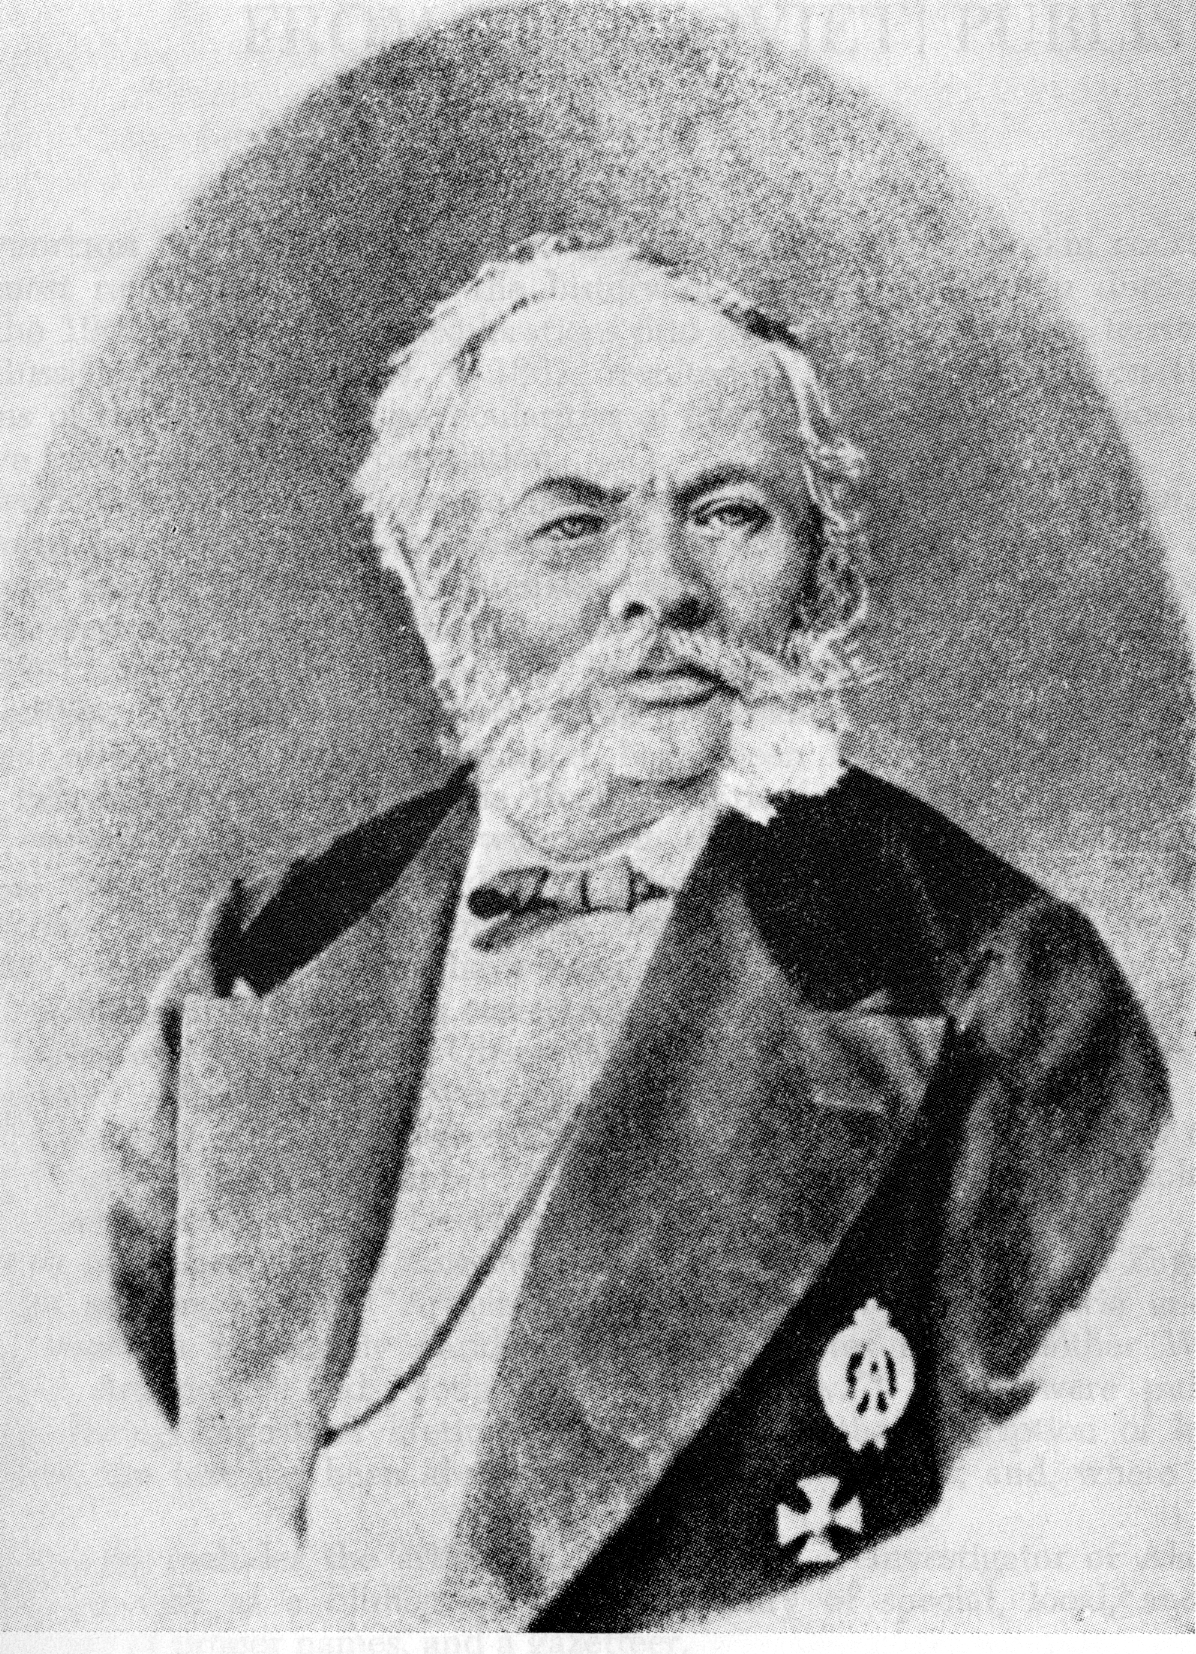
\includegraphics[width=0.6\textwidth]{figures/pratt-fig1}
    \caption{Portrait of Lavrentiy A. Zagoskin (from Chernenko et al. 1956 [Frontispiece])}
    \label{pratt-fig1}
\end{figure}

%\begin{center}
%    \begin{sideways}%[htbp]
%         \begin{minipage}{0.92\linewidth}
%                    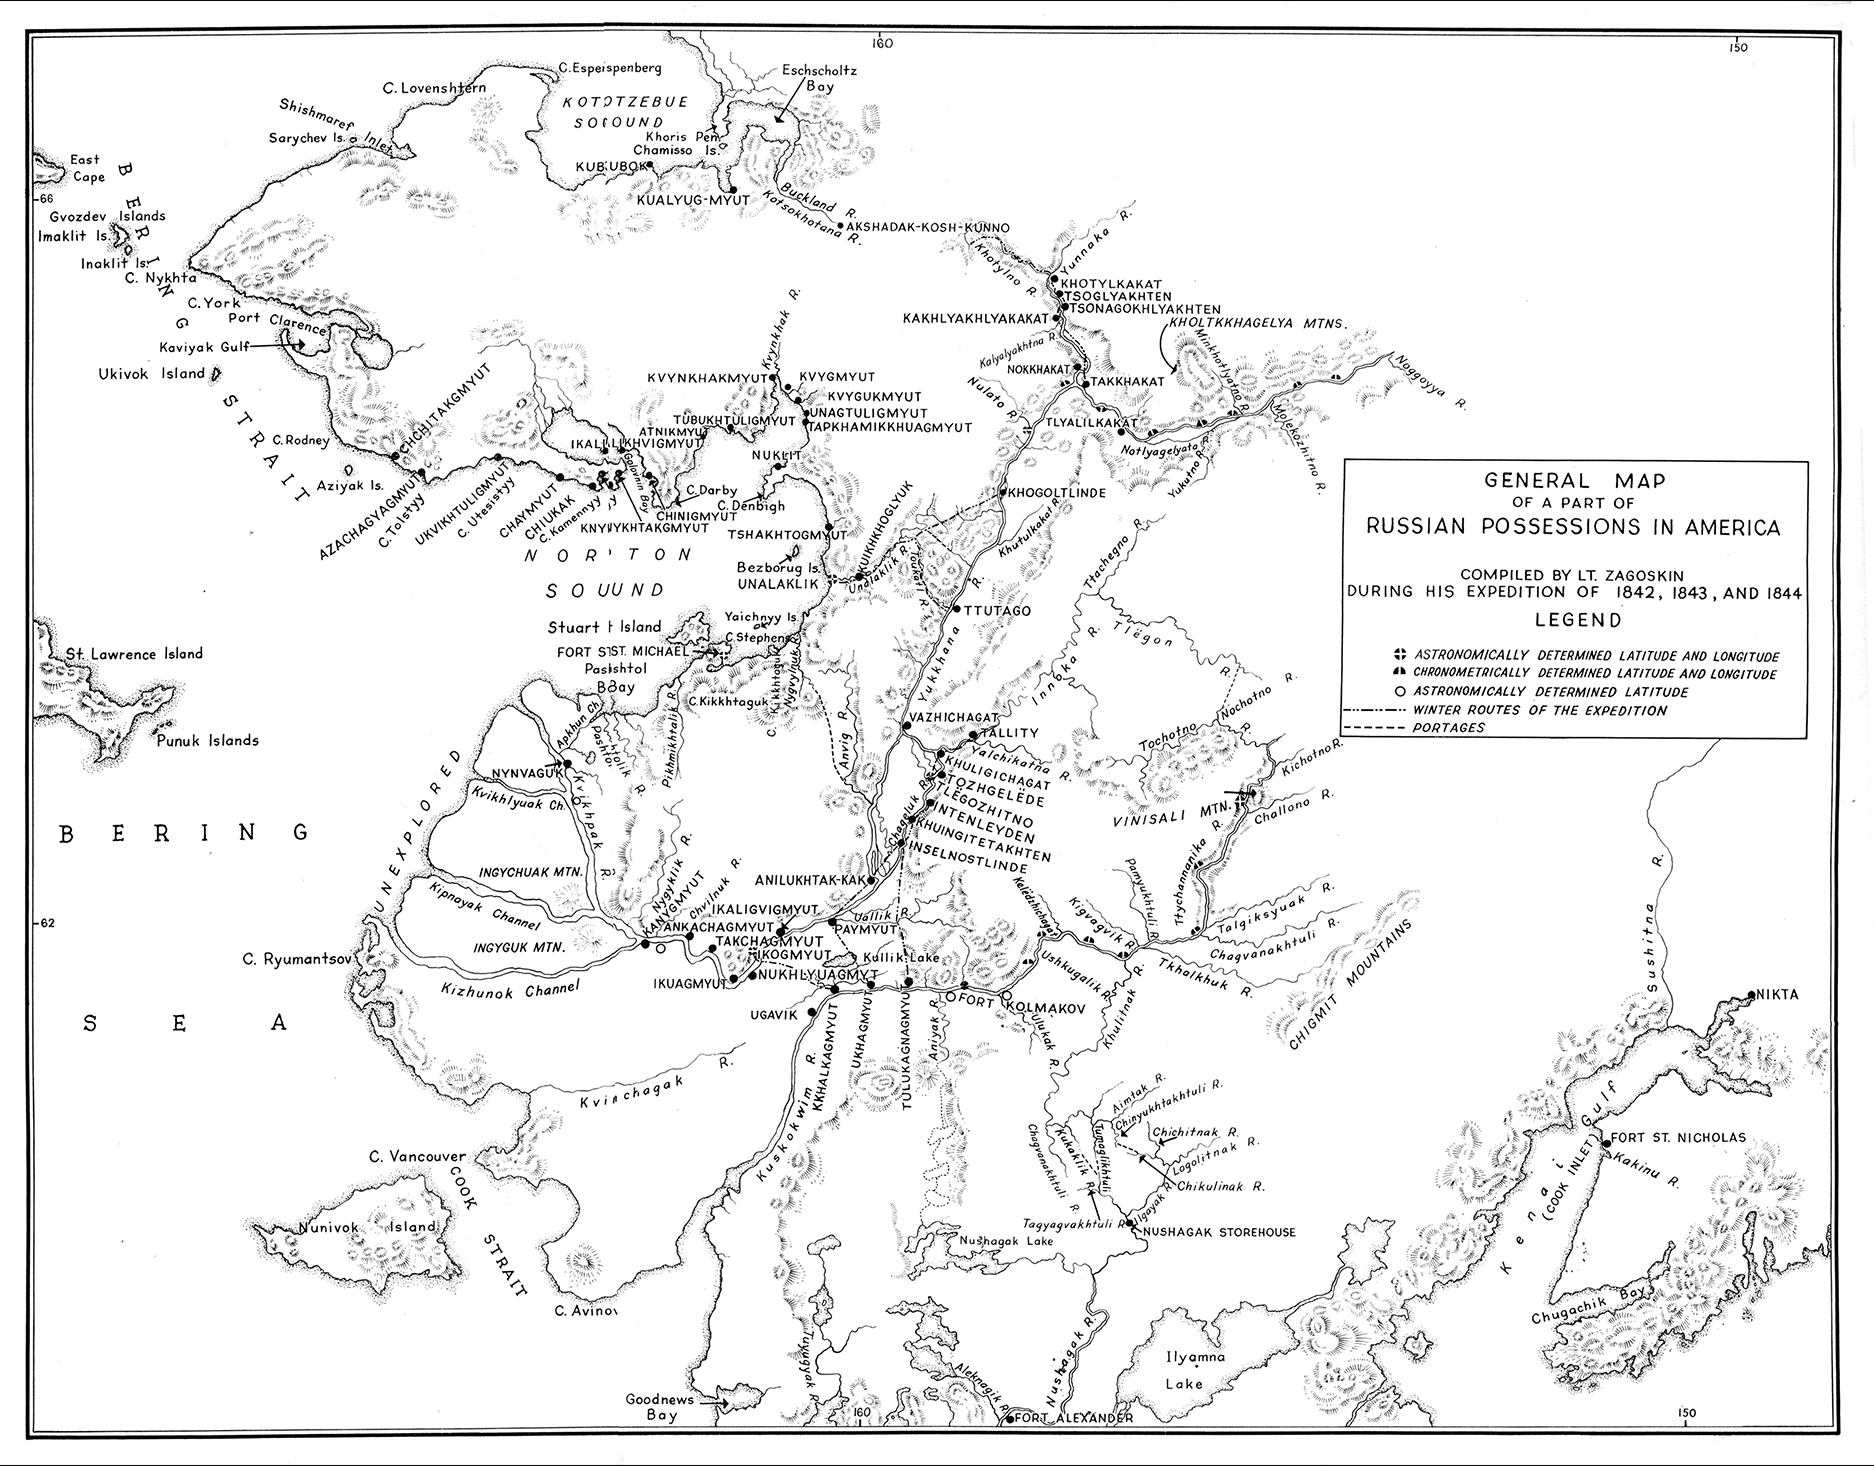
\includegraphics[width=\linewidth,keepaspectratio]{figures/pratt-fig2}
%                    \captionof{figure}{``General Map of a Part of Russian Possessions in America” (Zagoskin 1967 [facing p. 358])}
%         \label{pratt-fig2}
%         \end{minipage}
%    \end{sideways}
%    \end{center}
    
    \begin{figure}[!h]
    \centering
    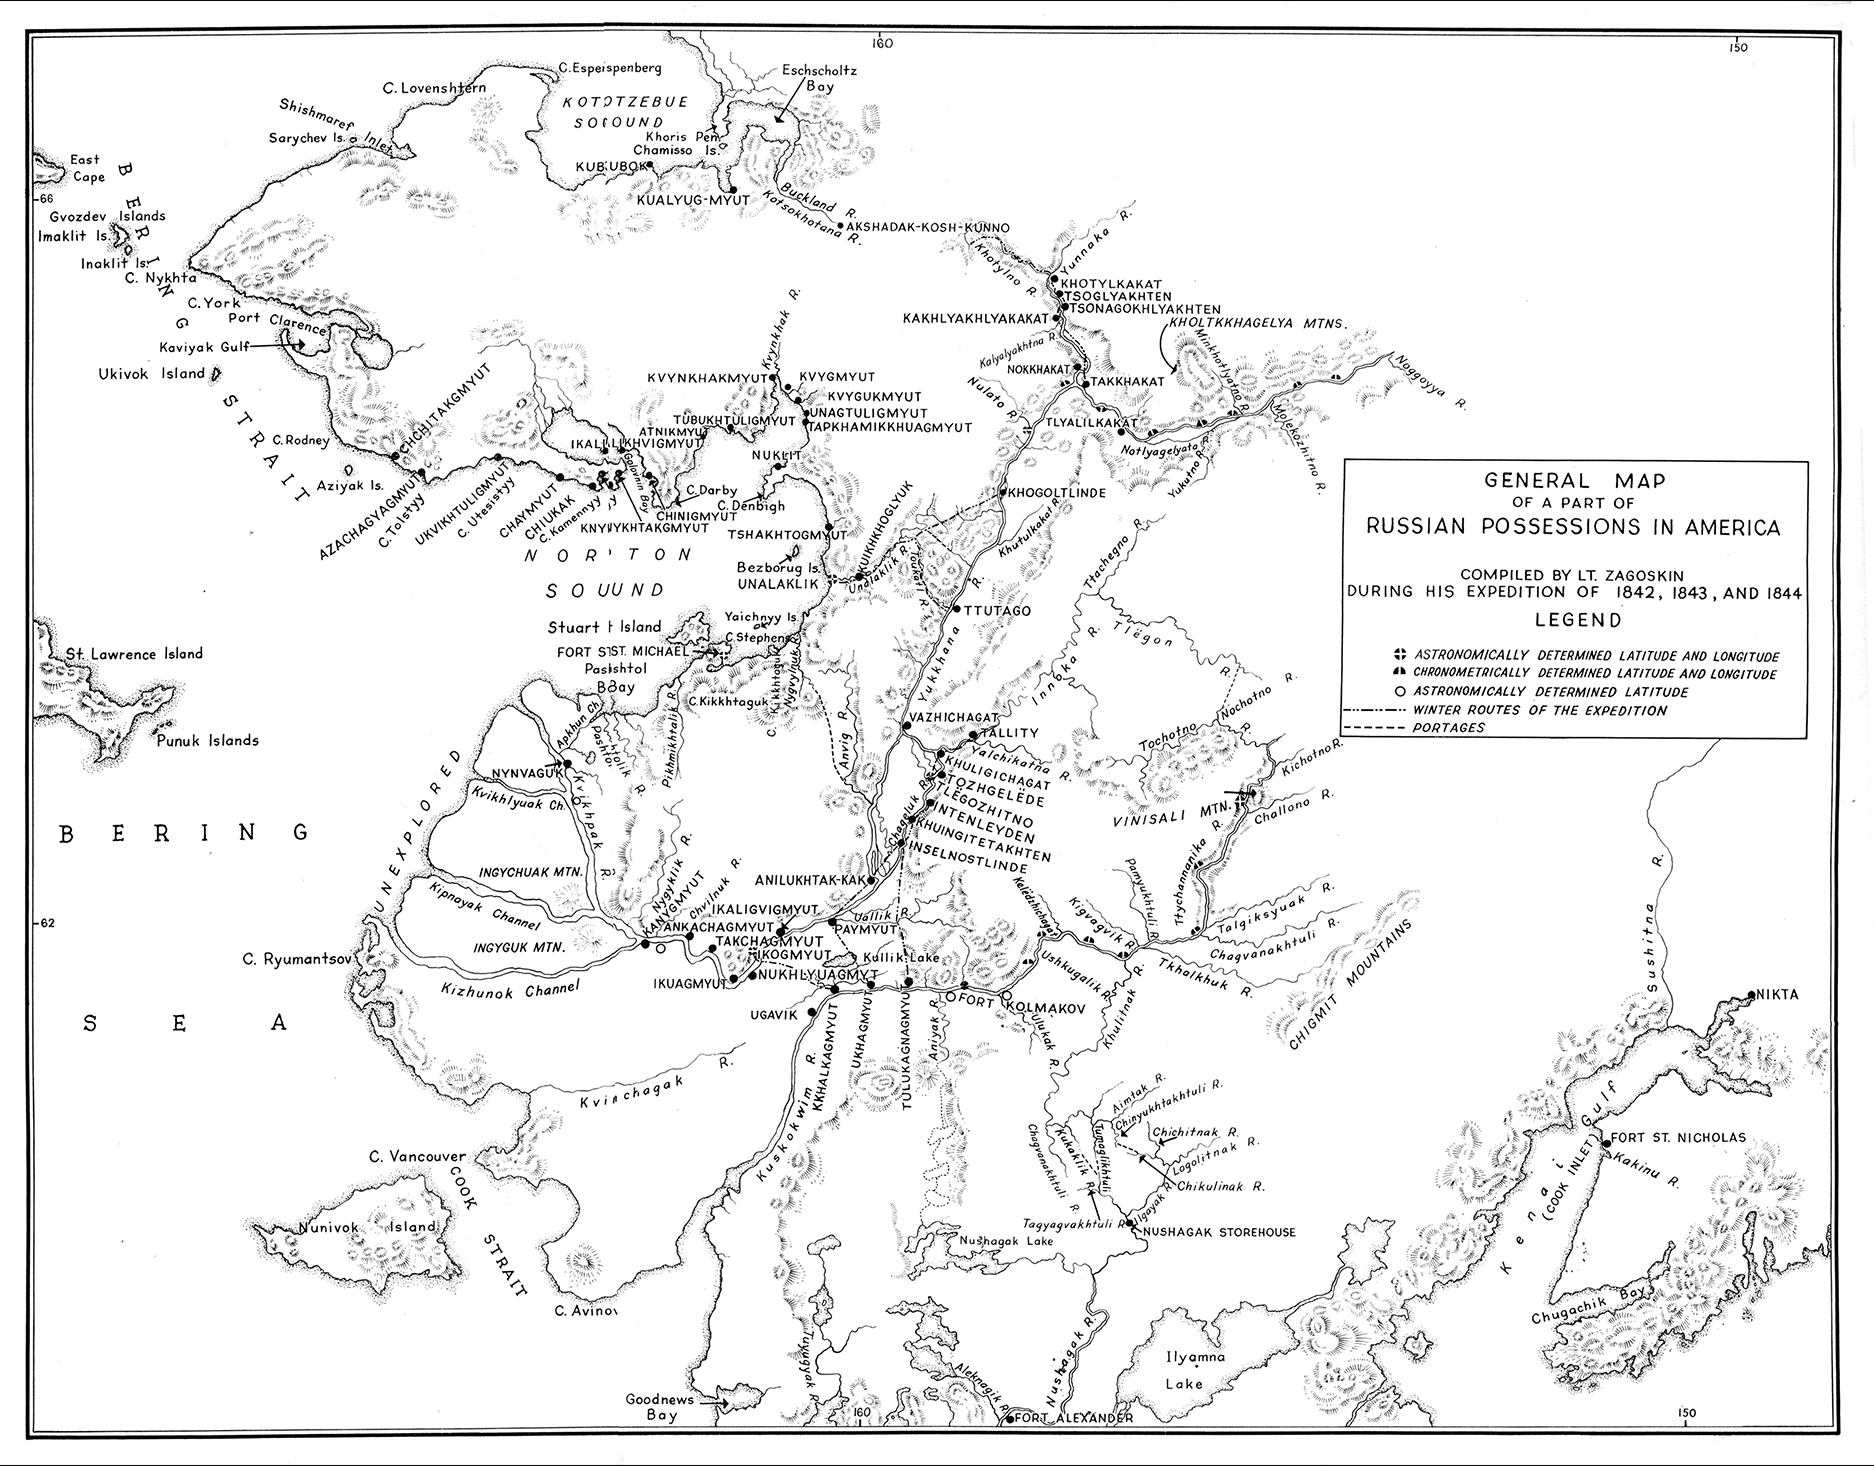
\includegraphics[width=\textwidth]{figures/pratt-fig2}
    \caption{``General Map of a Part of Russian Possessions in America” (Zagoskin 1967 [facing p. 358])}
    \label{pratt-fig2}
\end{figure}

\section*{Sociopolitical Setting}
The Zagoskin expedition was part of an effort begun in about 1818 by the Russian government and the Russian-American trading company to increase knowledge about the geography, resource wealth, and inhabitants of the Bering Sea coast and adjacent interior areas of “Russian America” [Alaska]. Because this region had not previously attracted serious attention from any foreign government the lifeways and traditions of its indigenous residents were intact, despite the presence of Euroamerican trade goods. Trade was, in fact, the main impetus for the expedition (see Arndt 1996: 52-54). A central expectation imposed on Zagoskin was to “find out by what routes furs were being exported from the interior of Alaska for [native] trade with the Chukchi [of Siberia] (Chernenko et al. 1956: 15). The ultimate Russian objective was to intercept furs that otherwise would be lost to established systems of aboriginal trade, such as that which flowed between the middle Yukon River and Norton Sound via the Kaltag Portage (e.g., see Pratt 2012). The collection of detailed information about Alaska Native peoples, their ways of life, and their knowledge of local and regional geography was key to this effort. Whether by accident or design, Zagoskin proved to be a good man for the task.

In both Eskimo and Athabascan populations of the region, the largest cohesive social unit of the Native peoples Zagoskin’s expedition encountered is best described as a “local group”: a somewhat fluid organization of one or more extended families that lacked formalized leadership positions and was centered around the same winter village. Each local group was economically self-sufficient. Its members followed a subsistence lifestyle that, based mainly on resource availability, involved moving between two to five different residence localities over the course of the year. The most populous locales were winter villages, which usually were occupied by two or more extended families for about six months at a time and ranged in population from about 25-100 residents. Historical accounts indicate some winter villages were substantially larger, but they were not common. Thus, in the normal routine of its travels the Zagoskin expedition came into contact with a wide array of small, autonomous Native groups whose relations with other nearby groups—as with their motivations relative to the Russians—could be highly variable. The sociopolitical landscape was complicated and potentially dangerous, thereby requiring careful and deliberate navigation by outsiders.

\section*{Data Collection Challenges on the Zagoskin Expedition}
Communication across language barriers is a critical and often overlooked factor to consider when evaluating ethnographic data about Native populations collected in any colonial setting. This is especially true when that process depended on interpreters, which was virtually always the case relative to nineteenth century Euroamerican explorations in Alaska’s Yukon and Kuskokwim River drainages (e.g., Pratt 2013: 23-25). Even Euroamericans who were comparatively skilled linguistically would have had difficulty communicating with Native groups in this region, as it was home to a number of distinct languages, most comprised of multiple dialects and sub-dialects. But Zagoskin is the only early explorer of the region who consciously alerted future readers of his account to linguistic constraints that affected the completeness and quality of the data he collected from and about Alaska Native peoples. Later visitors to the region (e.g., Edward W. Nelson [1899]) undoubtedly encountered similar problems but their works are generally accepted as historically valid without consideration of potential difficulties in cross-cultural communication—probably due in part to their lack of discussion of such issues. Another unique quality of Zagoskin’s work compared to those of other explorers of the region is that data he obtained directly from Alaska Natives were subjected to critical scrutiny and collected in accordance with a fairly strict methodology. Part of his approach was explained as follows:

\begin{quote}
    I have in general refrained from including information about places unknown to me, places which I could not check by personal observation, unless there was agreement in statements of several natives and an explanatory translation by an interpreter (Zagoskin 1967: 272).
\end{quote}

Zagoskin was in the region for just over two years in the early 1840s, during which time he made eleven separate trips (Pratt 1984: 120 [note 13])\footnote{Zagoskin arrived at St. Michael [Mikhailovskii Redoubt] on 10 July 1842 and departed from the same place for his return to Russia on 5 August 1844.  Chernenko ([1956] 1967: 19) presents a quote from Zagoskin’s diary that could be misread to suggest his tenure in Russian America was less than two years (i.e., “1 year, 6 months, and 16 days”), but it actually refers to the duration of time during which Zagoskin’s expedition was continuously away from St. Michael.} and used the services of at least eight different interpreters: i.e., five Russian Creoles\footnote{In Zagoskin’s usage, ‘Russian Creoles’ were “Those born in Russian America, sons and daughters of Russian fathers and [Alaska] native mothers” (Zagoskin 1967: 330). In the broader history of Russian America, however, the designation “creole” is more complicated (see Black 1990; 2004: 209-220). } and three Athabascan Indians (Pratt 1984: 135-137).  Two of the Athabascan interpreters were from the Koyukuk River area, and the other from the Yukon-Innoko River area. Of the Creole interpreters, two were from unspecified areas of Alaska; the others were from, respectively, Kodiak Island, Cook Inlet, and the Russian colony at Fort Ross, California.\footnote{“Stepanov,” the interpreter from Cook Inlet (Zagoskin 1967: 263, 345), was especially skilled and trusted by Zagoskin (1967:271-272; see also De Laguna 1947: 30). The interpreter from Kodiak Island was Nikifor Talizhuk, and the interpreter from Fort Ross was Pavel Agliaiuk (see Arndt 2015: 10-11). }

Zagoskin relied heavily on Russian post managers Andre Glazunov and Semen Lukin (both Creoles) for data about Yup’ik Eskimos (Zagoskin 1967: 143, 291-292 [note 41]; see also Oswalt 1990: 61). In fact, if his expedition ever specifically employed an Eskimo interpreter it is not clearly indicated in his journal.  But Zagoskin probably received some degree of linguistic aid from Yup’ik Eskimos of Unalakleet who guided him partway up the Unalakleet River (Zagoskin 1967: 133-135; see also Pratt 2012: 101-103); and from a Yup’ik woman [“Kuropatka”] who traveled with the expedition during a three-week trip between Russian Mission [“Ikogmyut”] and Nulato (Zagoskin 1967: 185-194). During the return leg of the latter trip he was also accompanied for a short period by Yup’ik residents of Paimiut (Zagoskin 1967: 194).

The most fundamental problem Zagoskin faced was simply communicating with his expedition—which he said was usually a composite of several Creoles, a few Eskimos and/or Athabascans, and maybe a fellow Russian or a Siberian Native [e.g., Nikitin, the “Tungus” (Zagoskin 1967: 103)].  Conversations with expedition members were generally conducted using a mixture of Russian, Athabascan and Eskimo, one consequence being that the interpreters “often failed to understand the gist of the questions put to them” (Zagoskin 1967: 167, 231).  This limited the information that could be transmitted during contacts with the region’s Native peoples, as indicated in the following statement.

\begin{quote}
    ...to avoid future criticism I feel that it is my duty to explain that all the information I collected here from the Tlegon-khotana [upper Innoko] Natives, as well as from those I met later on, came to me through the following system: every answer to my questions was given to Vtornik [a Koyukuk River Athabascan], who passed it on to Tatlek [another Koyukuk River Athabascan], who told it to the Creole interpreter from our California colony [Nikifor Talizhuk], who told it to me.  Thus, even a perfectly accurate piece of information could be distorted through the oral transfer between interpreters who barely understood each other (Zagoskin 1967: 168).

\end{quote}

Linguistic constraints explain Zagoskin’s reliance on material culture differences as his chief means for identifying and demarcating different Native groups during his expedition (e.g., Zagoskin 1967: 209). This is implied by a comment about his travels in the Koyukuk [“Yunnaka”] River area.

\begin{quote}
The difficulty of communicating through pantomime, and through three interpreters who often could not understand each other, often resulted in our limiting ourselves principally to questions about visible objects (Zagoskin 1967: 153, 295-296 [note 66]).
\end{quote}

\noindent
Zagoskin also noted the impact of language problems on his collection of Native places names.

\begin{quote}
    Our [Dene/Athabascan] guide…had an insufficient command of the [Eskimo] language spoken about us, and for this reason we were often unable to get satisfactory information from him, especially where renditions of place names was concerned (Zagoskin 1967: 232-233).

\end{quote}

\noindent
And also:

\begin{quote}
When we explored upstream [from Nulato] on the Yukon, we went through places where the Tlëgon-khotana people come down to the river, but as we did not have a proper interpreter we could not learn details about the crossing or the name of the river by which they cross (Zagoskin 1967: 300 [note 94]).
\end{quote}

After he had lived in both St. Michael and Nulato for some time, Zagoskin (1967:242) could somewhat understand the language of the former’s Eskimo and the latter’s Athabascan residents, and make himself understood to them (with some difficulty) “in a mixture of dialects.” Interestingly, he suggested that as his own Native language skills \textit{increased} his ability to record vocabulary terms from some groups \textit{decreased}---because his questions began to be answered almost exclusively in the dialects he understood (Zagoskin 1967: 242-243).

The expedition’s dependence on interpreters also forced Zagoskin to deal with the unwillingness of some interpreters to accompany his party into the homelands of groups with which they were unfamiliar or in areas they did not feel safe. One such instance involved the Koyukon Athabascan Tatlek’s reluctance to guide the party beyond the Koyukuk River mouth. Residents of that area warned Tatlek of potential danger in guiding Russians further up the Koyukuk, due to “the unfriendliness of the [Malemiut] and their antagonism towards [the Russians]” (Zagoskin 1967: 150). Zagoskin interpreted this warning as an obvious attempt by one group of traders to protect an avenue of their trade from another. Tatlek was uneasy, however, and only agreed to continue after being threatened with unpleasant consequences that would follow if he chose to abandon the party.

There were also occasions when Zagoskin felt the employment of guides and interpreters had negative effects on his meetings with Native peoples. He noted that when his party was not accompanied by guides or interpreters some groups “manifested a freer and friendlier attitude” and were “more communicative with words and signs”; conversely, he suggested some people’s timidity toward or reluctance to engage with his party “could be ascribed to the influence or attitudes of the guides, who always behave as though they had some sort of guardianship over us” (Zagoskin 1967: 176).

As the preceding comments suggest, Zagoskin’s journal contains numerous comments that describe difficulties in communication between his party and the local peoples with whom it came into contact. Nevertheless, he compiled a rich and remarkably accurate body of data about Native populations. His account is often the only and/or most important source of data available on some aspects of the region’s Native history (e.g., see Snow 1981: 605). Zagoskin’s conscientious documentation of place names (VanStone 1967b:xiii; see also Pratt 2012: 101-105) is a case in point.\footnote{Since the English translation of his journal (Zagoskin 1967) does not include an index, however, finding and extracting the place names data contained therein is a tedious task.} He was intent on collecting the Native names of settlements, hydrographic and topographic features encountered throughout the course of his expedition—and equally averse to applying Russian or honorific names to the landscapes through which he traveled. The latter practice was not followed nearly as rigidly by later explorers in the region. It is also noteworthy that the accounts of some individuals who arrived in the region after Zagoskin, spent more time there, and traveled extensively in connection with their duties (e.g., Iakov Netsvetov [1984]) suggest they devoted considerably less effort to documenting Native place names.

But Zagoskin did more than simply record such names—he also provided important contextual information for many of them. Three relevant examples follow. The first two apply to what is today known as the Innoko River (see Figure~\ref{pratt-fig3}).

\begin{quote}
    A little below [the settlement of Ttality] the river Ttachegno, flowing from the north, joins the Tlёgon. It is from the upper waters of the Ttachegno that the natives cross over to the Yukutno, and on it to the Yuna, or upper Yukon. After the junction of the Tlёgon and the Ttachegno, the river receives the name of Shiltonotno from the natives living in its upper reaches, and Innoka from the people living downstream. In general the direction of the channel is towards the southwest until it joins the Tstseyaka Slough, which flows from the Yukon. From this point…the river changes its name again and is called the Ittege by one tribe and Chagelyuk by the other (Zagoskin 1967: 237).
\end{quote}



\noindent
Here’s another example:

\begin{quote}
    It was 10 miles through woods and often over tundra to Khuligichagat village from the point we had determined, in the general direction of northwest 10°. Sometimes we traveled on the river, sometimes along its right bank. There is a small settlement called Tozhgelёde on the left bank of the Ittege 7 miles before one reaches Khuligichagat. The summer camp of this settlement is situated opposite one of the mouths of a channel which flows from the Yukon into the Ittege and which is called Tstseyaka by the natives. Along the trail we met five sleds and natives from the Iltenleyden settlement who were returning from the coast. They told us they had exchanged their furs at Kikkhtaguk [Klikitarik] village for sealskin and deerhide (Zagoskin 1967: 235).
\end{quote}

\noindent
And finally:

\begin{quote}
    The Talgiksyuak flows out of a small lake. Its width at high water is from 30 to 50 sazhens,\footnote{A \textit{sazhen} is a measure of length equal to 2.1 meters. } in the fall only half of this. Otter are caught here in great numbers, and the fish as they come upstream—whitefish, muksun whitefish, and imagnat [blackfish]. The winter camp of Chinik is situated at its mouth; there are more than 10 camps of the Ikogmyut and Ikaligvigmyut along the river (Zagoskin 1967: 274).
\end{quote}

Linguistic applications notwithstanding, critical analysis of this associated place names information can help researchers to: (a) determine the locations of many of the named places on modern topographic maps; (b) reconstruct Native subsistence and land use patterns; and (c) delineate certain ethnic group boundaries extant at the time of Zagoskin’s expedition. With respect to the last, Zagoskin recognized (1967:298 [note 76], 299 [note 89]) that different groups often had different names for the same river, place or feature (Table~\ref{pratt-tab1}; see also Figure~\ref{pratt-fig4}). When such dual names were recorded he gave precedence to “the local names as a clearer indication of the location of different tribes” living in the area (Zagoskin 1967: 295 [note 65]).


\begin{table}
	\centering
	\small
	\label{pratt-tab1}
	\caption{Selected Athabascan and Eskimo Place Names Reported by Zagoskin, with Known Modern Equivalents.}
	\begin{tabular}{ L{1.5cm} L{4cm} L{3cm} L{3cm} }
\toprule
\textbf{Feature Type}&\textbf{Athabascan~Name}&\textbf{Eskimo~Name}&\textbf{Modern~Name}\\
\midrule
Site&Inselnostlende&Katykhkatmyut&\\
Site&Khuingitetakhten&&\\
Site&Iltenleyden&Unagun-chagelyugmyut&Shageluk\\
Site&Khuligichagat&&Holikachuk\\
Site&Vazhichagat, Makaslat&&\\
Site&Ttality, Totaskholëden&&Dementi\\
Site&&Anilukhtakpak&Gost Creek \\
Site&&Paymyut&Old Paimiut\\
River& \makecell[tl]{Tlëgon [upper] \\ Innoka, Shiltonotno [middle]\\ Ittege [lower] }
          &Chagelyuk&Innoko River\\
River&Yalchikatna&Tachaychagat&Iditarod River\\
River&Tstseyaka [upper]&&Thompson Slough, Holikachuk Slough\\
River&Tstseyaka&&Shageluk Slough\\
River&&Uallik&Paimiut Slough\\
River&\makecell[tl]{Yuna\\Yukkhana}&Kvikhpak&Yukon River\\
River&\makecell[tl]{Ttykini\\Ttychannanika}&Kuskokwim&\makecell[tl]{Kuskokwim River\\Upper Kuskokwim}\\
River&Khottylno&Kvikhchagpak&Crooked Creek\\
River&Kholitna, Khulitnak&&Holitna River\\
River&Khochalitno&Chagvanakhtuli&Swift River\\
River&Talgatno&Talgiksyuak&Tatlawiksuk River\\
		
\bottomrule		
		
	\end{tabular}
\end{table}


Detailed observations by Zagoskin about local environmental landscapes through which his party passed sometimes provide deeper contexts for certain Native place names. His remarks about the “Innoka” River are a case in point.

\begin{quote}
    The extraordinary width of the [Yukon] river is certainly explained by the speed and the enormous quantity of water which pours into it during the spring floods from all its tributaries. As all these waters cannot be contained in the channel, they wash away and cut into the banks, creating the innumerable islands which we found between Nulato and Vazhichagat. Below this point the Yukon displays another surprising peculiarity: when the Tstseyaka and other sloughs split off from it, more than half of its waters flow into the Innoka, creating various low but sizeable islands which are dotted with lakes stocked with fish (Zagoskin 1967: 195).
\end{quote}
\noindent
This description expands Jette’s (n.d.:110-111) later explanation of the Innoko (i.e., Lurno [“fish river”]) place name, which was summarized by the following statement: “The Innoko River is remarkable for the abundance of fish in its waters, hence its name.”

\section*{Concluding Remarks}
The importance of Zagoskin’s work is clearly recognized by numerous scholars who have used and become familiar with the journal of his expedition (e.g., Arndt 1996: 59-65; Bockstoce 2009: 194-196; Brooks 1953: 232-234; De Laguna 1947: 29 [note 19], 31; Orth 1967: 43-44; Oswalt 1967: 233; VanStone 1967b; 1979b:78). I count myself among that group, having likely used the report of Zagoskin’s expedition more extensively than any other scholar—both for personal research (e.g., Pratt 1984, 2012) and in my official capacity documenting Alaska Native cultural sites (see Pratt 2009)—and consistently finding his data to be highly reliable. Unfortunately, Zagoskin was harshly criticized by William H. Dall (1877:22; cf. De Laguna 1947: 29 [note 19], 31; 2000: 33-34), whose opinion on the subject is at best ironic given the dubious accuracy of some of his own work (see Arndt 1996: 177; Petroff 1884: 161; Ray 1975: 133-134; VanStone and Goddard 1981: 561). Youthful arrogance was likely a factor, but Dall’s criticism of Zagoskin may also have been influenced by the general disdain he seemed to hold for Russians in Alaska (e.g., see De Laguna 2000: 187-188). Less understandable is the fact that Zagoskin has also been maligned by several prominent scholars who arguably did not make serious efforts to utilize his account (i.e., Black 1984: 30 [see also Netsvetov 1984:xx; cf. Oswalt 1990: 59-61]; Burch 1984: 9).\footnote{In his last major publication, Burch (2012) put considerable stock in Zagoskin’s observations about caribou in western Alaska. True to his penchant for scholarly honesty, when questioned about his 1984 criticism of Zagoskin versus his new reliance on the explorer’s account Burch (personal communication, 2/10/2010) explained that his original, negative impression was based on comments about Zagoskin’s work received from a respected colleague.} One indirect goal of this paper is to objectively challenge and counteract these negative assessments of Zagoskin’s report. Another is to make the point that problems involving cross-cultural communication—although rarely mentioned—arguably posed greater challenges to the success of early Euroamerican explorers of the Yukon-Kuskokwim region than did the physical hardships they encountered.

This brief summary of Zagoskin’s work provides a foundation for critically reviewing the Native place names data he collected. Minimally, any such review should include at least three tasks.

\begin{enumerate}

    \item  Searching the writings of other early authors and more recent sources relevant to the geographical area of focus to determine if some of the same places for which Zagoskin recorded names are represented in their works.
    \item Critically comparing locational information provided by Zagoskin about specific named places against modern topographical maps in an effort to accurately correlate the names with discrete places on the physical landscape.\footnote{Henry N. Michael, editor of the 1967 English translation of Zagoskin’s journal, did a remarkably good job in his own efforts to make such correlations—particularly considering his lack of personal knowledge of the regions of Alaska visited by Zagoskin’s expedition. Another benefit of this comparative task is that it sometimes reveals significant errors on published United States Geological Survey (USGS) maps. The present case yielded several examples of such errors (e.g., refer to the place names “Kakyglët” and “Kukaklik Lake” in the Appendix). Finally, in 2010 and 2011 Russian explorer Mikhail Malakhov organized and led expeditions to Alaska that followed routes taken by nineteenth century Russian explorers along the Yukon-Kuskokwim Portage and an overland trail between the Kuskokwim and Nushagak Rivers. The expedition’s findings were helpful in resolving several problematic correlations with place names reported by Zagoskin.}
    \item Undertaking the necessary linguistic research to correct (consistent with accepted Alaska Native language orthographies), or at least improve, place name spellings Zagoskin reported.
\end{enumerate}

Although none could be done in a truly comprehensive fashion, each of the tasks just described was essential to producing the Appendix to this paper. It lists place names found in Zagoskin’s comparatively short accounts of his trips between the Yukon River village of “Ikogmyut” (Russian Mission), the Innoko River and upper Kuskokwim River from November 1843 to June 1844 (see also Figures~\ref{pratt-fig5} and \ref{pratt-fig6} in the Appendix). The 45 journal pages that describe those trips (i.e., Zagoskin 1967: 199-208, 231-242, 249-274) reference 145 named places: most are identified with Native place names, reflecting multiple languages (e.g., Central Yup’ik, Deg Xinag, Holikachuk, Koyukon, Upper Kuskokwim, Dena’ina). Significantly, my findings suggest that about half of these place names do not appear in Donald Orth’s (1967) encyclopedic Dictionary of Alaska Place Names. This underscores the great potential Zagoskin’s 300+ page journal holds for increasing the current inventory of Native place names in Alaska.


\section*{Acknowledgements}
I wish to thank Jim Kari for his generous help and sharing of data associated with my efforts to correlate and correct spellings of certain Native place names recorded by Zagoskin; Robert Drozda, Matt O’Leary and Mikhail Malakhov for assistance related to the Appendix; Dale Slaughter for his work on the maps contained herein; Katherine Arndt for providing me with biographical information about the namesake of “Slatin post”; an anonymous reviewer for helpful comments on a draft of the paper; and Gary Holton for inviting me to contribute to this volume.


\refheading
\begin{hang}

Anvil, Oscar. 1988. Tape recorded oral history account. Ted Krieg, interviewer; Mary Gregory, interpreter. Bethel, Alaska; 6 July. Tapes 88CAL053 and 88CAL054. Bureau of Indian Affairs, ANCSA Office, Anchorage.

Arndt, Katherine L. 1996. \textit{Dynamics of the Fur Trade on the Middle Yukon River, Alaska, 1839 to 1868}. Ph.D. dissertation, Department of Anthropology, University of Alaska Fairbanks.

Arndt, Katherine L. 2015. Transplanted to a Northern Clime: Californian Wives and Children in Russian Alaska. \textit{Alaska Journal of Anthropology} 13(2). 1-20.

Arundale, Wendy H. 1983. \textit{Doyon Historic Sites Project Report: Innoko Area}. Doyon, Limited, Fairbanks. (Copy on file at Bureau of Indian Affairs, ANCSA Office, Anchorage.)

Black, Lydia T. 1984. The Yup’ik of Western Alaska and Russian Impact. \textit{Etudes/Inuit/Studies} 8 (Supplementary Issue). 21-43.

Black, Lydia T. 1990. Creoles in Russian America. \textit{Pacifica} 2(2). 142-155.

Black, Lydia T. 2004.	\textit{Russians in Alaska, 1732-1867}. University of Alaska Press, Fairbanks.

Bockstoce, John R. 2009. \textit{Furs and Frontiers in the Far North: The Contest among Native and Foreign Nations for the Bering Strait Fur Trade}. Yale University Press, New  Haven and London.

Brooks, Alfred H. 1953. \textit{Blazing Alaska’s Trails}. University of Alaska Press, Fairbanks.

Burch, Ernest S., Jr. 1984. The Central Yup’ik Eskimos: An Introduction. \textit{Etudes/Inuit/Studies} 8 (Supplementary Issue). 1-19.

Burch, Ernest S., Jr. 2012. \textit{Caribou Herds of Northwest Alaska, 1850-2000}. Edited by Igor Krupnik \& Jim Dau. University of Alaska Press, Fairbanks.

Chernenko, Mikhail Borisovich. 1967[1956]. Lavrentiy Alekseyevich Zagoskin: An Account of His Life and Works.  In Henry N. Michael (ed.), \textit{Lieutenant Zagoskin’s Travels in Russian America, 1842-1844}, 3--34. Translated by Penelope Rainey.  University of Toronto Press, Toronto.

Chernenko, M.B., G.A. Agranat \& Y.E. Blomkvist. 1956. \textit{The Travels and Explorations of Lieutenant Lavrentiy Zagoskin in Russian America, 1842-1844}. State Publishing House of Geographic Literature, Moscow.

Dall, William H. 1877. \textit{Tribes of the Extreme Northwest}. Contributions to North American Ethnology, Vol. 1. Government Printing Office, Washington, DC.

De Laguna, Frederica. 1947. \textit{The Prehistory of Northern North America as Seen from the Yukon}. Memoirs of the Society for American Archaeology, Number 3. Menasha, WI.

De Laguna, Frederica. 2000. \textit{Travels among the Dena: Exploring Alaska’s Yukon Valley}. University of Washington Press, Seattle and London.

Ellanna, Linda J. \& Andrew Balluta. 1992. \textit{Nuvendaltin Quht’ana: The People of Nondalton}. Smithsonian Institution Press, Washington, DC and London.

Fienup-Riordan, Ann (ed.). 1988. \textit{The Yup’ik Eskimos: As Described in the Travel Journals and Ethnographic Accounts of John and Edith Kilbuck, 1885-1900}. Edited, with an Introduction by Ann Fienup-Riordan. Limestone Press, Kingston, ON.

Fienup-Riordan, Ann (ed.). 2014. \textit{Nunamta Ellamta-llu Ayuqucia (What Our Land and World Are Like): Lower Yukon History and Oral Traditions}. Translated and Transcribed by Alice Rearden; edited by Ann Fienup-Riordan. Calista Elders Council (Anchorage) and Alaska Native Language Center, University of Alaska Fairbanks.

Grinev, Andrei. 2009. \textit{Kto est’ kto v istorii Russkoi Ameriki [Who is who in the history of Russian America]}. Academia, Moskva.

Hosley, Edward H. 1981. Kolchan. In June Helm (ed.), \textit{Handbook of North American Indians, vol. 6: Subarctic}, 618-622. Washingon, DC: Smithsonian Institution Press.

Ignati, Evan. 1994. Tape recorded oral history account. Robert Drozda, interviewer. Fairbanks, Alaska; 28 October. Tape 94HOL001.RD. Copy on file, Bureau of Indian Affairs, ANCSA Office, Anchorage.

Jette, Jules. n.d.	On the Geographical Names of the Ten’a. “Jottings of a Missionary,” unpublished manuscripts, Alaska Mission Collection, M/F 96, roll 34, Rasmuson Library Archives, University of Alaska Fairbanks.

Kari, James (ed.). 2015. \textit{Upper Kuskokwim Athabascan Place Names Lists}. Unpublished manuscript, Alaska Native Language Center, University of Alaska Fairbanks.

Kari, James \& James A. Fall. 2003. \textit{Shem Pete’s Alaska: The Territory of the Upper Cook Inlet Dena’ina} (2nd edition). University of Alaska Press, Fairbanks.

Kari, Priscilla Russell. 1983. \textit{Land Use and Economy of Lime Village}. Technical Paper No. 80, Alaska Department of Fish and Game, Division of Subsistence, Juneau.

Kari, Priscilla Russell. 1985. \textit{Wild Resource Use and Economy of Stony River Village}. Technical Paper No. 108, Alaska Department of Fish and Game, Division of Subsistence, Juneau.

Malakhov, Mikhail. 2011a.	Kuskokwim-Yukon-63K-MalakhovRoute (map). \url{https://cloud.mail.ru/public/9nV9/okP5Zt7oK}

Malakhov, Mikhail. 2011b	Nushagak-Kuskokwim-250K-MalakhovRoute (map). \url{https://cloud.mail.ru/public/CAm8/z4RByjM2r}


Mikhail, Gusty. 1980. Kuskokwim River Place Names (interview). Jim Kari, interviewer and transcriber (with Yup’ik names transcribed by Steve Jacobson). Stony River, Alaska; 23 November. Tape Ik14. Fairbanks: Alaska Native Language Archive.

Nelson, Edward W. 1899.	\textit{The Eskimo about Bering Strait}. Bureau of American Ethnology, 18th Annual Report, part 1, 1896-97. Government Printing Office, Washington, DC.

Netsvetov, Iakov. 1984. \textit{The Journals of Iakov Netsvetov: The Yukon Years, 1845-1863}. Translated, with an Introduction and Supplementary Material by Lydia T. Black. Edited by Richard A. Pierce. Limestone Press, Kingston, ON.

Orth, Donald J. 1967. \textit{Dictionary of Alaska Place Names}. Geological Survey Professional Paper 567. Government Printing Office, Washington, DC.

Osgood, Cornelius. 1958.	\textit{Ingalik Social Culture}. Yale University Publications in Anthropology, no. 53. Yale University Press, New Haven, CT.

Oswalt, Wendell H. 1967. \textit{Alaskan Eskimos}. Chandler Publishing Company, San Francisco.

Oswalt, Wendell H. 1980. \textit{Historic Settlements along the Kuskokwim River, Alaska}. Alaska State Library Historical Monograph No. 7, Juneau.

Oswalt, Wendell H. 1990. \textit{Bashful No Longer: An Alaskan Eskimo Ethnohistory, 1778—1988}. University of Oklahoma Press, Norman and London.

Petroff, Ivan. 1884. \textit{Report on the Population, Industries, and Resources of Alaska: Tenth Census of the U.S.A., 1880}. Government Printing Office, Washington, DC.

Phillip, Joshua. 1988. Tape recorded oral history account. Robert Drozda, interviewer; Vernon Chimegalrea, interpreter. Tuluksak, Alaska; 29 June. Tape 88CAL046. Bureau of Indian Affairs, ANCSA Office, Anchorage.

Porter, Robert P. 1893. \textit{Report on the Population and Resources of Alaska at the Eleventh Census: 1890}. Government Printing Office, Washington, DC.

Pratt, Kenneth L. 1984. Yukon-Kuskokwim Eskimos, Western Alaska: Inconsistencies in Group Identification.  M.A. thesis, Department of Anthropology, Western Washington University, Bellingham.

Pratt, Kenneth L. 2012. Reconstructing 19th-Century Eskimo-Athabascan Boundaries in the Unalakleet River Drainage. \textit{Arctic Anthropology} 49(2). 14-112.

Pratt, Kenneth L. 2013. Deconstructing the Aglurmiut Migration: An Analysis of Accounts from the Russian-America Period to the Present. \textit{Alaska Journal of Anthropology} 11(1-2). 17-36.

Pratt, Kenneth L. (ed.). 2009. \textit{Chasing the Dark: Perspectives on Place, History and Alaska Native Land Claims}. Edited by Kenneth L. Pratt. U.S. Department of the Interior, Bureau of Indian Affairs – Alaska Region, ANCSA Office, Anchorage.

Ray, Dorothy Jean. 1975. \textit{The Eskimos of the Bering Strait, 1650-1898}. University of Washington Press, Seattle and London.

Smith, Louis. 1990. Tape recorded oral history account. Mary Ellen Fogarty, interviewer; Marie Meade, interpreter. Goodnews Bay, Alaska; March 9. Tape 90PLA005. Bureau of Indian Affairs, ANCSA Office, Anchorage.

Snow, Jeanne H. 1981. Ingalik. In June Helm (ed.), \textit{Handbook of North American Indians, vol. 6: Subarctic}, 602-617. Washington, DC: Smithsonian Institution Press.

Townsend, Joan B. 1965. \textit{Ethnohistory and Culture Change of the Iliamna Tanaina}. Ph.D. dissertation, Department of Anthropology, University of California Los Angeles. University Microfilms, Inc., Ann Arbor.

United States, Bureau of Indian Affairs (USBIA). 1991a.	Report of Reinvestigation for Old Paimiut, AA-12370 (Doyon, Limited). Written by Ronald J. Kent \& Matthew O’Leary. Bureau of Indian Affairs, ANCSA Office, Anchorage.

United States, Bureau of Indian Affairs (USBIA). 1991b.	Report of Investigation for Khuingitetakhten, AA-12363 (Doyon, Limited). Written by Ronald J. Kent, Thomas J. Turck \& Debra Corbett. Bureau of Indian Affairs, ANCSA Office, Anchorage.


United States, Bureau of Indian Affairs (USBIA). 2008. Supplemental Report for Island Village, AA-12360 (Doyon, Limited). Written by Rita A. Miraglia. Bureau of Indian Affairs, ANCSA Office, Anchorage.

VanStone, James W. 1967a.	\textit{Eskimos of the Nushagak River: An Ethnographic History}. Seattle: University of Washington Press.

VanStone, James W. 1967b.	Introduction.  In Henry N. Michael (ed.), \textit{Lieutenant Zagoskin’s Travels in Russian America, 1842-1844}, xi--xiv. Translated by Penelope Rainey.  University of Toronto Press, Toronto.

VanStone, James W. 1978. \textit{E.W. Nelson’s Notes on the Indians of the Yukon and Innoko Rivers, Alaska}. Edited with an introduction by James W. VanStone. Fieldiana Anthropology, Volume 70. Field Museum of Natural History, Chicago.

VanStone, James W. 1979a.	\textit{Historic Ingalik Settlements along the Yukon, Innoko, and Anvik Rivers, Alaska}. Fieldiana Anthropology, Volume 72. Field Museum of Natural History, Chicago.

VanStone, James W. 1979b.	\textit{Ingalik Contact Ecology: An Ethnohistory of the Lower-Middle Yukon, 1790—1935}. Fieldiana Anthropology, Volume 71. Field Museum of Natural History, Chicago.

VanStone, James W. (ed.). 1988. \textit{Russian Exploration in Southwest Alaska: The Travel Journals of Petr Korsakovskiy (1818) and Ivan Ya. Vasilev (1829)}. Edited with an Introduction by James W. Vanstone; translated by David H. Kraus. University of Alaska Press, Fairbanks.

VanStone, James W. \& Ives Goddard. 1981. Territorial Groups of West-Central Alaska before 1898. \textit{Handbook of North American Indians, vol. 6: Subarctic}. Washington, DC: Smithsonian Institution Press.

Williams, Sinka \& Stanley Nook. 1988. Tape recorded oral history account. Philippa Coiley, interviewer. Lower Kalskag, Alaska; 20 July. Tape 88CAL081. Bureau of Indian Affairs, ANCSA Office, Anchorage.

Wright, Miranda. 1995. The Last Great Indian War (Nulato, 1851). M.A. thesis, Department of Anthropology, University of Alaska Fairbanks.

Zagoskin, Lavrentiy A. 1967. \textit{Lieutenant Zagoskin’s Travels in Russian America, 1842-1844: The First Ethnographic and Geographic Investigations in the Yukon and Kuskokwim Valleys of Alaska}.  Translated by Penelope Rainey; edited by Henry N. Michael.  University of Toronto Press, Toronto.


\end{hang}

\vspace{1cm}
\orcidfooter{Kenneth L. Pratt}{kenneth.pratt@bia.gov}{}



%%%%%%%%%%%%%%% appendix follows %%%%%%%%%%%%%%%%%%%%%%%

\clearpage
\noindent
\textbf{\large Appendix: Place Names} \\


\noindent
This Appendix lists the 145 named places mentioned by Zagoskin in four of his party’s trips, the combined accounts of which cover a total of 45 pages in his journal. Place names are listed in the order they were reported during each trip—with the caveat that each place name is listed only once (on the first occasion of its mention). Thus, a place name mentioned in all four of the trips being considered would only appear below in connection with the first trip.



The place name spellings provided in Zagoskin’s journal are \hl{boldfaced}\todo{bolding is copied from the original word document}, with any translations he reported following in parentheses. Italicized place names denote Native language spellings. When known, the Alaska Native language of origin for a place name is indicated by one of the following abbreviations: CY (Central Yup’ik), DH (Deg Hit’an), D (Dena’ina), H (Holikachuk), K (Koyukon), or UK (Upper Kuskokwim). Time limitations precluded any serious attempt to gather and compile place name translations. The feature type to which a given place name is attached is noted; so are correlations to locales (see Figures~\ref{pratt-fig5} and \ref{pratt-fig6}, hydrographic or topographic features named on modern United States Geological Survey (USGS) maps.



In a number of cases, extra contextual information Zagoskin recorded about places named in his account has been included to give readers a better overall sense of the range of information collected during his Alaska travels. Zagoskin's remarks are often supplemented with related comments by the author.


\vspace{1cm}
\noindent
\textbf{Trip 1: Ikogmyut to Fort Kolmakov [23 November – 6 December 1843]
(Zagoskin 1967: 203-208 [22 place names])}
\vspace{6pt}

\begin{hang}

\textbf{Ikogmyut} [\textit{Iqugmiut} (CY)]: winter village, and site of the Russian post Ikogmyut Odinochka (est. 1835); present-day Russian Mission.



\textbf{Kuskokwim}: watercourse; USGS Kuskokwim River.



\textbf{Fort Kolmakov}: Kolmakovskii Redoubt (est. 1832); located on left (south) bank of Kuskokwim River opposite the mouth of USGS Kolmakov River (see Oswalt 1980: 90 [Map 3]).



\textbf{Paymyut} [\textit{Paimiut} (CY)]: winter village; Old Paimiut, abandoned ca. 1880s. Historically, this was the uppermost Eskimo village on the Yukon River. (Note: the site Zagoskin visited is not USGS Paimiut—which was established in the mid-1930s, is located on the opposite (i.e., right) bank of the Yukon, and is the most recent of five sites in the immediate vicinity that were all known as “Paimiut.”)



\begin{quote}“Paymyut ...is situated on the left bank at the confluence of the Yukon and the Uallik. From this village there is an all-year trail to the Kuskokwim” (Zagoskin 1967: 194). The trail referred to here was the Yukon-Kuskokwim Portage.
\end{quote}



\textbf{Yukon}: watercourse; USGS Yukon River.



\textbf{Kkhalkagmyut} [\textit{Qalqarmiut} (CY)]: winter village; Old Kalskag, abandoned ca. 1915 (Oswalt 1990: 122; see also Oswalt 1980: 71-72). This site is located downriver from present-day Lower Kalskag and is not depicted on USGS maps.



\textbf{Ikaligvigmyut} (“fishy”) [\textit{Iqallugvigmiut} (CY)]: winter village; USGS Dogfish Village.



\textbf{Uallik River} [\textit{Ualiq} (CY)]: watercourse; USGS Paimiut Slough.



\textbf{Pashtol} [\textit{Pastuliq; Pastuliarraq} (CY)]: winter village; USGS Pastolik. A major Yup’ik Eskimo village located near the north mouth of the Yukon River; abandoned ca. 1963.



\textbf{Tashatulit}: mountains; USGS Portage Mountains.



\textbf{Ingytkvyygat} (“mountain stream”): watercourse; location uncertain.



\textbf{Tulukagnagmyut} (“crow”) [\textit{Tulukarnermiut} (CY)]: USGS Crow Village. According to Oswalt (1980:38), “In early historic times this was the farthest inland village along the Kuskokwim of exclusively Yupik-speaking Eskimos.”



\textbf{Ukhagmyut} [\textit{Urr’armiut} (CY)]: winter village; USGS Ohogamiut (on Kuskokwim River).



\textbf{Fort Alexander}: Aleksandrovskii Redoubt (est. 1819), located on Nushagak Bay at the mouth of Nushagak River. Also sometimes called the “Nushagak post” (e.g., Zagoskin 1967: 241).\textbf{ }



\textbf{Nushagak}: winter village; Native village at the mouth of Nushagak River (the same location at which Alexandrovskii Redoubt was established).



\textbf{Nuskagak Lakes}: this term of reference likely applied to all of the lakes in the USGS Wood River Lakes and USGS Tikchik Lakes systems.



\textbf{Nushagak}: lake; USGS Tikchik Lake (VanStone 1988: 95).



\textbf{Aniak River} [\textit{Anyaraq} (CY)]: watercourse; USGS Aniak River.



\textbf{Innoka} [\textit{Eniq, Enigg }(DH) \textit{or Yoonig} (H) (Arundale 1983: 48): watercourse. In Zagoskin’s usage this is the middle section of USGS Innoko River.



\textbf{Kukhlyukhtakpak} (“big waterfall”): a camp of the people of Kvygympaynagmyut located on the left bank of Kuskokwim River just downstream from present-day Chuathbaluk (see Oswalt 1980: 48 [“Kukuktuk”], 90 [Map 3]). Zagoskin (1967:232) also identified the site as the “Kukhlyukhtakpak trail house” when his party overnighted there before embarking on the overland trail from the Kuskokwim to the lower Innoko River.



\textbf{Kvygympaynagmyut} [\textit{Kuigem Paingarmiut} (CY)] (also \textbf{Kvygympayma} [\textit{Kuigem Painga} (CY)]: winter village; located on right (north) bank of Kuskokwim River at mouth of USGS Kolmakov River (opposite “Fort Kolmakov”). Also the site of “Lukin’s Odinochka”—built in 1833, the forerunner of Kolmakovskii Redoubt (e.g., Oswalt 1990: 50-51).



\textbf{Fort St. Michael}: Mikhailovskii Redoubt (est. 1833), located on St. Michael Island in southern Norton Sound, at the site of \textit{Taciq}, a Yup’ik Eskimo winter village.

\end{hang}


\vspace{1cm}
\noindent
\textbf{Trip 2: Fort Kolmakov to the Lower Innoka River and Return to Ikogmyut [10 February – 25 March 1844] (Zagoskin 1967: 231-242 [46 place names])}
\vspace{6pt}

\begin{hang}
\textbf{Ittege} [\textit{Edixi} (DH) [Eter’e (Jetté n.d.:83-84)]: watercourse. In Zagoskin’s usage this is the lower section of USGS Innoko River. (\textit{Edixi} = the ‘upper area’ name for the Shageluk village area [Jim Kari, personal communication, 11/28/2015].)



\textbf{Tachatalyatna}: watercourse (a ‘mountain stream’); location uncertain.



\textbf{Anilukhtakpak} [DH]: winter village; USGS Gost Creek, located on the left bank of USGS Walker Slough near present-day Holy Cross (see VanStone 1979a:61-62).



\begin{quote}“[Anilukhtakpak is] the last settlement of the Ttynay [Dene (Athabascan)] on the Yukon: farther downstream and on all the branches of this river, on the Kuskokwim flats, and along the coast to the Alaska Peninsula the people are of the Kang-yulit [Eskimo] tribe” (Zagoskin 1967: 193).
\end{quote}



\textbf{Kykhtulit} [\textit{Digheloye Chin} (UK)]: mountains; “western piedmont, edge of Alaska Range above treeline” (Kari 2015: 13 [no. 168]). Also referred to as “the Kykhtulit Range” (e.g., Zagoskin 1967: 251-252).



\begin{quote}Kykhtulit was described as the ridge that “divides the basin of the Kuskokwim from the waters of Nushagak” (Zagoskin 1967: 232).
\end{quote}



\textbf{Chuazhutl}: mountain group; location uncertain.



\textbf{Tagasushku}: mountain group; location uncertain.



\textbf{Nantlinde}: mountain group; location uncertain.

\begin{quote}
	“The mountain range which stretches northward from the Tashatulit [Portage Mountains] mass to the left bank of the Ittege can be seen at a distance of 25 to 30 miles from the [Yukon-Kuskokwim Portage] trail. Separate mountain groups are called by the natives Chuazhutl, Tagasushku, and Nantlinde. The Uallik [Paimiut Slough] has its source on the slopes of the first two of these groups” (Zagoskin 1967: 232).
\end{quote}



\textbf{Kullik} (“trousers”) [\textit{Qerrulliik} (CY)]: watercourse [“one of the tributaries of the Uallik” (Zagoskin 1967: 233)]; probably USGS Twelvemile Slough.



\textbf{Kauvak}: camp; location uncertain.



\textbf{Naumgyk}: watercourse [a small river “which falls into one of the tributaries of the Uallik” (Zagoskin 1967: 233)].



\textbf{Inselnostlende} [DH] or \textbf{Katykhkatmyut} [CY]: winter village. As confirmed by BIA ANCSA researchers in 2007, the site location is on the right bank of Innoko River about 20 miles south of Shageluk. The site corresponds with Osgood’s (1958:30) “Island-Village” and apparently Jetté’s “Ekarotsor” (VanStone 1979a:17).



\textbf{Khuingitetakhten} [DH]: winter village. As confirmed by BIA ANCSA researchers in 1986, the site location is on the left bank of Innoko River about 12 miles south of Shageluk.



\textbf{Iltenleyden} [\textit{Niłteghelinghdi} (DH)] or \textbf{Unagun-chagelyugmyut} [CY]: winter village; USGS Shageluk. See Arundale (1983:39-40), De Laguna (1947:64 [Fig. 14]), and VanStone (1979a:17-18).



\textbf{Tlëgozhitno} [\textit{Łeggi Jitno’} (DH)]: winter village; Old Shageluk (Arundale 1983: 41-45 [“Segment C”]; see also VanStone 1979a:18-22; 1979b:77 [Fig. 5]).



\textbf{Tlëgozhitno} [\textit{Łeggi Jitno’} (DH)]: watercourse; unnamed on modern maps, this was a tributary of the “Tstseyaka” (USGS Shageluk Slough).



\begin{quote}
“Near Tlëgozhitno [village] a stream of the same name detaches itself from the Tstseyaka and flows into the Ittege” (Zagoskin 1967: 235 [see also map, facing p. 358]). This description indicates Henry Michael was mistaken in saying that “[Tlëgozhitno] is a local name for the lower reaches of the Innoko” (see Zagoskin 1967: 356).
\end{quote}



\textbf{Tstseyaka} [\textit{Ts’ooyeekk’e} (K), \textit{Ts’ooyegg} (H), \textit{Ts’eyegg} (DH)]: watercourse; USGS Shageluk Slough. This is the southernmost of two channels of the same watercourse, both identified as “Tstseyaka” by Zagoskin.



\textbf{Khuligichagat} [\hl{\textit{HəyeẏeləNdə}} (H)]: winter village; USGS Holikachuk.

\todo[inline]{I copied the Holikachuk from the word document, though I wonder if the uppercase N is meant to indicate an engma (ŋ). The dotted-y presumably to indicate voiced uvular fricative [ʁ]. Could be easier to cite the practical orthography Xiyighelinghdi. }


\textbf{Tozhgelëde}: winter village; Tigshelde (Orth 1967: 966, 980). [“The summer camp of this settlement is situated opposite one of the mouths of a channel which flows from the Yukon into the Ittege and which is called Tstseyaka by the natives” (Zagoskin 1967: 235)].



\textbf{Kikkhtaguk} [\textit{Qikertaq} (CY)]: USGS Klikitarik, a Yup’ik Eskimo winter village on southern Norton Sound.



\textbf{Vazhichagat} [DH] or \textbf{Makaslag} (Zagoskin 1967: 191 [K]): winter village. Zagoskin’s map (1967, facing p. 358) depicts this site on the left bank of the Yukon River just upstream from the mouth of Tstseyaka [the northern channel (i.e., USGS Thompson Slough, Holikachuk Slough)]. VanStone (1979a:53) stated that efforts by De Laguna (in 1935) and himself (in 1972 and 1974) failed to locate the site, so it was thought to have been destroyed by riverbank erosion. Jim Kari (personal communication, 11/16/2015) suggested this may be Jetté’s (n.d.) \textit{Maats’e Kkaagget}; however, it seems clear that the latter site was situated on the opposite (right) bank of the Yukon near the mouth of USGS Grayling River (e.g., De Laguna 1947: 65).



\begin{quote}“All the natives living on the Ittege travel to the coast both in summer and winter by way of Vazhichagat, then along a mountain stream that flows into the Yukon; almost at the latitude of the village they reach the upper waters of the Anvig; from there the trail continues in the same direction followed by Glazunov on his first trip in 1835. The crossing from Vazhichagat to Kikkhtaguk takes about three days under normal conditions” (Zagoskin 1967: 191).
\end{quote}



\textbf{Nulato}: Nulato Odinochka ( est. 1839-1840), site of the famous “Nulato Massacre” in 1851 (e.g., De Laguna 2000: 162-188; Wright 1995); also a Koyukon Athabascan village (i.e., Nulato [\textit{Noolaahe Doh} (K)]).



\textbf{Ttality} (“fast current”) or \textbf{Totaskholëden}: village; USGS Dementi. Located on the right bank of Innoko River opposite the mouth of USGS Iditarod River (Orth 1967: 266, 980; Snow 1981: 615; VanStone 1978: 65 [note 22]).[



\begin{quote}“By night we reached the village of Ttality or Totaskholëden, the first settlement [on the Innoko] of the Tlëgon-khotana tribe, or Inkalikhlyuat, that is the ‘Far Inkalit’” (Zagoskin 1967: 236). Also referred to as the “Innoka-khotana,” this designation applied to “the tribe living along the upper Innoka and its tributaries. Along the Tlëgon River this same tribe calls itself the Tlëgon-khotana, in all likelihood referring by this to the place where they had been settled originally” (Zagoskin 1967: 242).
\end{quote}


\textbf{Tlëgon} \textbf{River} [\textit{Łoooghunh} (H), \textit{Łeghunh} (DH), \textit{Łighen} (D), \textit{Tlooghunh} (K)]: watercourse. In Zagoskin’s usage this is the upper section of USGS Innoko River; [the “principal source” of the Innoka River (Zagoskin 1967: 237)]. Previously identified by Petr Kolmakov as the “Legon” (Zagoskin 1967: 353), this watercourse corresponds with the Luron or Lurno (“fish river”) of Jetté (n.d.:8, 12, 110-111).



\textbf{Tlëgon} [\textit{Łoooghunh} (H), \textit{Łeghunh} (DH), \textit{Łighen} (D), \textit{Tlooghunh} (K)]: winter village; apparently located in the vicinity of USGS Davenport (Henry Michael, in Zagoskin 1967: 237, 356; Snow 1981: 615)



\textbf{Tochotno} [\textit{Tochotno’} (UK)]: watercourse; USGS Takotna River. This marks the furthest upstream point on the Kuskokwim reached by Zagoskin’s party (see Zagoskin 1967: 271-272).



\textbf{Nochotno} [\textit{Nets’in Tazdlinh} (Nixon Fork) (UK)]: watercourse; USGS Nixon Fork [Takotna River] (Orth 1967: 692).



\textbf{Ttachegno}: watercourse [river, which “flowing from the north, joins the Tlëgon” (Zagoskin 1967: 237)]; USGS North Fork [Innoko River] (Orth 1967: 699, 988).



\textbf{Yukutno} [\textit{Yooggutno’} (K) (Jetté n.d.)]: watercourse; USGS Yuki River (Jim Kari, personal communication, 11/28/2015).



\textbf{Yuna} [\textit{Yoona’} (K)]: watercourse; the “upper Yukon” River (Zagoskin 1967: 237).



\textbf{Shiltonotno}: watercourse. In Zagoskin’s usage, this was the middle section of USGS Innoko River.



\textbf{Tstseyaka Slough} [\textit{Ts’ooyeekk’e} (K), \textit{Ts’ooyegg} (H), \textit{Ts’eyegg} (DH)]: watercourse [``…the upper mouth of the Tsteyaka, the channel to the Yukon” (Zagoskin 1967: 236)]; USGS Thompson Slough, Holikachuk Slough. (Note: the southern channel of this watercourse (also identified as “Tstseyaka”) corresponds to USGS Shageluk Slough.)



\textbf{Chagelyuk} [\textit{Caarrilluk} (CY)]: watercourse. In Zagoskin’s usage this was the lower section of USGS Innoko River.



\textbf{Tlegokokhkakak} [\textit{Łook’a kux kagg} (H and K)]: winter village; located “Along the banks of the [Innoko] river between Tlëgon and Ttality” (Zagoskin 1967: 237-238).



\textbf{Tleket}: winter village; located “Along the banks of the [Innoko] river between Tlëgon and Ttality” (Zagoskin 1967: 237-238).



\textbf{Kkholikakat} [\textit{Qaleka\.g} (H)]: winter village; located on the left bank of Innoko River at or near the mouth of USGS Hammer Creek (Snow 1981: 615).



\textbf{Yalchikatna} or \textbf{Tachaychagat River}: watercourse; USGS Iditarod River [“…the most outstanding…of the principal tributaries that flow into this [middle] course of the Innoka” (Zagoskin 1967: 238)].



\begin{quote}“The Tochotno is made up of several mountain streams that flow out of the eastern slope of the mountains from which the Tachaychagat flows from the west. We discussed the difficulty of the portage between the upper waters of these two streams” (Zagoskin 1967: 271). (The prior discussion of this portage is found on pages 253-254 of Zagoskin’s journal.)
\end{quote}



\begin{quote}“The entire country drained by the Innoka and its tributaries, with the exception of the Innoka’s lower reaches, is inhabited by the tribe of Inkalit Yug-elnut” (Zagoskin 1967: 238). This tribal designation encompassed Athabascan residents of the “Yukon from Blackburn to Holy Cross, the lower Innoko below Shageluk-Thompson Slough, and the lower Kuskokwim below the “Holitno River” and above the Eskimo at the delta” (De Laguna 1947: 30; Zagoskin 1967: 242).
\end{quote}



\textbf{Anvig}: winter village; located on the Yukon River’s right bank at the mouth (left bank) of USGS Anvik River (see De Laguna 1947: 67-68; 2000: 270).



\textbf{Takchilkilyagmiut} [CY]: village; located on the Yukon River about 10 miles downstream from the mouth of Innoko River (see Zagoskin 1967: 355)—probably on USGS Horse Island near the north mouth of USGS Big Bend Slough.



\textbf{Novoarkhangelsk}: Novo-Arkhangel’sk, located at present-day Sitka. Established as a post in 1799, it was destroyed by Tlingit warriors in 1802 and rebuilt by the Russians in 1804, after which date it served as the capital of Russian America.



\textbf{Kadyak}: island; USGS Kodiak Island. Also the location of a Native village of the same name and several Russian trade posts.



\textbf{Norton Sound}: gulf.

\end{hang}

\vspace{1cm}
\noindent
\textbf{Trip 3: Ikogmyut to Fort Kolmakov [4 April – 10 June 1844]   (Zagoskin 1967: 249-263 [32 place names]) }
\vspace{6pt}

\begin{hang}

\textbf{Talgiksyuak} [\textit{Taallerviksaq} (CY)]: watercourse; USGS Talbiksok River.



\textbf{Amylkinokh}: watercourse; location uncertain.



\textbf{Klek} [\textit{Kliq} (CY)]: watercourse. Unnamed on modern maps, this is a tributary to USGS Talbiksok River; its confluence with the Talbiksok is in Sec. 30, T. 18 N., R. 66 W., Seward Meridian.



\textbf{Tumyagak}: watercourse; location uncertain.



\textbf{Kakyglët} [\textit{Kakeggluk} (CY)]: watercourse; USGS Johnson River. This place name’s correlation with Johnson River is based on: (a) Zagoskin’s (1967:274) statement that Kukaklik Lake is the source of the Kakyglët; (b) Orth’s (1967:476) statement that Johnson River “heads in a lake 2 mi. W of [USGS] Kukaklik Lake”; and (c) the fact that the lake referenced by Orth is Zagoskin’s (1967:274) “Kukaklik Lake.”



\begin{quote}
    “The river Kakyglët is not over 3 \textit{sazhens} wide and is also quite deep. There are about 10 groups of Kkhalkagmyut dwellings situated along it” (Zagoskin 1967: 274). The designation “Kkhalkagmyut” refers to the residents of Old Kalskag (\textit{Qalqarmiut}).
\end{quote}


\begin{quote}
“We passed the night on the Kakyglët, which flows into the Kvinchagak (Zagoskin 1967: 250).
\end{quote}


\textbf{Kvinchagat} [\textit{Kuicaraq} (CY)] [also spelled “Kvinchagak”]: watercourse; USGS Crooked Creek. This place name’s correlation with Crooked Creek is based on: (a) Zagoskin’s (1967:274) detailed description of the route of the Yukon-Kuskokwim Portage trail; and (b) his paired explanation that “Kullik Lake” is the source of the Kvinchagat, into which the Kakyglët flows.\\

{\setlength{\parindent}{0em}
*Note that USGS Crooked Creek [here interpreted to be the “Kvinchagat”] and USGS Johnson River [here interpreted to be the Kakyglët] do, in fact, join one another (at a point consistent with Zagoskin’s [1967:274] description)—and either could reasonably be interpreted as flowing into the other. The latter point is partially expressed by the fact that \textit{Kuicaraq} (“Kvinchagat”) is the Native name for USGS Johnson River (“Kakyglët).
}


\begin{quote}“The natives say the source of the Kvinchagak is in Kullik Lake. Along its tributaries they hunt otter, muskrat, and beaver” (Zagoskin 1967: 274).
 \end{quote}





\textbf{Cape Avinov}: point of land; USGS Cape Avinof (located in the Kuskokwim Bay area).



\textbf{Cape Count Rumyantsev}: point of land; USGS Cape Romanzof (located at the western end of USGS Askinuk Mountains).



\textbf{Bristol Bay}: gulf.



\textbf{Bezymyannaya} [Russian for “Nameless” (Henry Michael, in Zagoskin 1967: 251)]: watercourse. In the sections of Zagoskin’s journal covered by this paper this is the only instance in which a Russian name was applied to a feature of the physical landscape. Zagoskin (1967:251) said it was only designated as such because his party ”knew no other name for it” and explained that the watercourse was “made up of many mountain streams flowing down the ravines of hills along the left bank [of the Kuskokwim].” The implication is that this watercourse was fairly substantial in size.



\textbf{Khulitnak} [\textit{Haghelitnu} (D), \textit{Xaletno’} or \textit{Xoletno’} (DH), \textit{Uulitna} (CY)]: watercourse; USGS Holitna River (same as Khulitna). [“Khulitnak, or in the dialect of the Ttynay tribe the Kholitno” (Zagoskin 1967: 267).]



\textbf{Ulukak} [\textit{Ulukaq} (CY)]: watercourse; USGS Holokuk River.



\textbf{Kvygym} [\textit{Kuigem} (CY)]: watercourse; USGS Kolmakov River.



\textbf{Chugunakhchugvik} [CY]: mountains; USGS Horn Mountains.



\textbf{Kvilkhak} [CY]: watercourse; USGS Portage Creek [\textit{Yutnalluki}].



\textbf{Kolmakov}: located on Holitna River at or near its confluence with Portage Creek, this was a resting place and trans-shipment point for Russian trade goods and supplies (like the “Nushagak trail-house” [below]) on the travel route from Kolmakovskii Redoubt on the Kuskokwim and Alexandrovskii Redoubt on the Kenai Peninsula. Established in 1832, it was also known as “Kolmakov’s Odinochka”(e.g., Oswalt 1990: 48-50). This was also the site of an Eskimo village, the name of which Zagoskin (1967:254) recorded as “Ukhvigchagvagmyut.”



\textbf{Ukhvigchagvagmyut} [CY]: winter village (Native name for the Holitna River site of Kolmakov).



\textbf{Tumaglikhtuli} [CY]: watercourse; location uncertain.



\textbf{Agyagat} \textbf{River} [CY]:\textbf{ }watercourse; location uncertain.



\textbf{Tagyagvakhtuli} [CY]: watercourse; location uncertain.



\textbf{Nushagak trail-house}: Russian post, also known as the “Nushagak Odinochka.” It was apparently in use by 1835 and functioned primarily as “a resting place and trans-shipment point” for trade goods and supplies on the travel route between Kolmakovskii Redoubt on the Kuskokwim River and Alexandrovskii Redoubt on the Kenai Peninsula (VanStone 1967a:51-52). Its precise location is uncertain but likely was “at or near the mouth of what is today called the King Salmon River” (VanStone 1967a:52).



\textbf{Ilgayak River}: watercourse; Yup’ik Eskimo name for the upper Nushagak River (i.e., upstream from its confluence with the Nuyakuk River [VanStone 1971: 27]).



\textbf{Aimtak} [\textit{Ayemtaaq} (CY)]: watercourse; USGS Shotgun Creek [the Khulitnak’s “chief tributary” [Zagoskin 1967: 254]), the name of which is based on the Native name’s translation (i.e., “shotgun”).



\textbf{Uksyuakhchullik River}: watercourse; location uncertain [“a tributary of the Chichitnak” (Zagoskin 1967: 254)]



\textbf{Chichitnak}: watercourse; USGS Chichitnok River. This place name is said to be a “Yupik version of very early Dena’ina name, with hydronym \textit{–tnak}” (Jim Kari, personal communication, 11/28/2015).



\textbf{Chinyukhtakhtuli} [CY]: watercourse; location uncertain [“a tributary of the Aimtak” (Zagoskin 1967: 254)].



\textbf{Ugavik} [\textit{Uaravik} (CY)]: winter village; USGS Uknavik. The site was evidently abandoned by the early 1920s (Fienup-Riordan 1988: 503-504; see also Oswalt 1980: 68-69).



\begin{quote}Zagoskin (1967:254) reported that, as of 1844, the Manager of Fort Kolmakov kept “a temporary post for trading with the tribes of the lower [Kuskokwim] river [at Ugavik], but he has not decided to visit that area himself, out of consideration for the great number of natives there and their turbulent character.”
\end{quote}



\textbf{Tkhalkhuk} [\textit{Teggalquq} (CY)] or \textbf{Mantashtano} [D]: watercourse; USGS Stony River. The Stony River is apparently known as \textit{Giqedhatno’} or \textit{Gidighuyghatno’} to the Deg Hit’an. Also, Jim Kari (personal communication, 11/28/2015) has noted that the name “Mantashtano” (\textit{Ven Dashtnu} [D]) refers to USGS Stink River, which flows into Stony River about 24 miles southeast of the Stony’s confluence with Kuskokwim River (Orth 1967: 919).



\textbf{Chukvak} [CY]: summer camp; probably present-day Chuathbaluk (see Oswalt 1980: 35-36).



\textbf{Sitka}: Russian post, and Native village. In context, “Sitka” here refers to Novo-Arkhangel’sk rather than to the community of Sitka, per se.



\textbf{Kanlkuchak} [CY]: summer camp; at/near (or possibly opposite) present village of Napaimiut. Said to be “situated 7 miles upstream from [Fort Kolmakov]” (Zagoskin 1967: 261).

\end{hang}

\vspace{1cm}
\noindent
\textbf{Trip 4: Fort Kolmakov to the Upper Kuskokwim and return to Ikogmyut [May 19 - June 10, 1844] (Zagoskin 1967: 263-274 [45 place names])}
\vspace{6pt}


\begin{hang}

\textbf{Kybgakhtuk} (“forest” [Zagoskin’s translation]) [\textit{Kevraartuq} (CY, “spruce tree”)]: summer camp. Probably located at stream mouth on right (north) bank of Kuskokwim River at extreme right edge of T. 17 N., R. 53 W., Seward Meridian. This camp was said to be “Three miles [above/upstream] from the fort [Kolmakovskii Redoubt]” (Zagoskin 1967: 264; cf. Oswalt 1980: 62 [“Napamiut \#1”], 90 [Map 3]).



\textbf{Ikalikhtuli} [CY]: winter village; USGS Little Mountain village.



\textbf{Chugunakhchugvik} [CY]: summer camp. Probably located at mouth of unnamed stream [also known as Chugunakhchugvik?] that heads in the Horn Mountains and reaches the Kuskokwim River in T. 18 S., R. 50 W., Seward Meridian (opposite the “Horn Village” of Oswalt [1980:42]).



\textbf{Ushkugalik} [\textit{Uskuralek} (CY)]: winter village; USGS Oskawalik.



\textbf{Kvikhchagpak} [CY]: summer camp; at or near present village of Crooked Creek.



\begin{quote}“The Kvikhchagpak summer camp is located on the right bank of the Kuskokwim at the mouth of a fairly large river…” [i.e., the Khottylno/Kvikhchagpak] (Zagoskin 1967: 265).
\end{quote}



\textbf{Khottylno} (“sharp turn” [DH?] [“Inkalit Yug-elnut”]) or \textbf{Kvikhchagpak} (“big stream” [UK (“in the Kuskokwim dialect”)]): watercourse; USGS Crooked Creek.



\textbf{Kelëdzhichagat}: summer camp; at or near the present village of Georgetown (e.g., Oswalt 1980: 41). [“In the two years of our travels, we never came upon a more pleasant place” (Zagoskin 1967: 266)]



\begin{quote}“The name [Kelëdzhichagat] reveals that this place has been settled by the Inkalit Yug-elnut who migrated to Kvygympayma village from the Innoka” [Zagoskin 1967: 266]).
\end{quote}



\textbf{Kelëdzhichagat}: watercourse; USGS George River. [“From the source of this stream there used to be a crossing to the Innoka, but since the beaver moved away the trail has been abandoned” (Zagoskin 1967: 266)].



\textbf{Agalitnak River}: watercourse; USGS Hoholitna River (see Orth 1967: 424). The Agalitnak is “a tributary of the Kholitno” (Zagoskin 1967: 266). The Hoholitna River is reportedly known as \textit{Tleghtitnu} to the Dena’ina (Ellanna and Balluta 1992: 326).



\textbf{Ttykini}: watercourse; USGS Kuskokwim River.



\begin{quote}“The Ttynay of the Yug-elnut tribe call the Kuskokwim Ttykini” (Zagoskin 1967: 266).
\end{quote}



\textbf{Tlyagenadëden}: village; correlated with present-day Parks by Orth (1967:739), but may actually be downstream in the vicinity of USGS Willis Creek. Zagoskin (1967:266) described its location as about 10 miles “south of [upstream from] the Kelëdzhichagat summer camp.”



\textbf{Yklyk} (“Burned”): mountain; USGS Barometer Mountain.



\textbf{Ttychannanika} [\textit{Dichina Nek’} (UK)]: watercourse; the upper Kuskokwim River. Zagoskin’s map (1967, facing p. 358) applies this name to the Kuskokwim above the Stony River.



\begin{quote}The Upper Kuskokwim “is called ‘Ttychannanika’ by the Ttynay-Goltsan tribes living along it” (Zagoskin 1967: 267). In the anthropological literature, the people Zagoskin designated the “Ttynay-Goltsan” are today known as the “Kolchan” (e.g., see Hosley 1981: 622).
\end{quote}



\textbf{Ingvagvik}: watercourse; location uncertain, but apparently situated along the “eastern channel” of the Ttychannanika about 7 miles northeast of its confluence with the Khulitnak [Holitna] (see Zagoskin 1967: 267). Possibly the river that flows into the right (north) bank of the Kuskokwim opposite sand bars in the lower quarter of T. 19 N., R. 42 W., Seward Meridian.



\textbf{Takhvalkynakat} [\textit{Tixveł Viniq’it} (D)]: “a cove or backwater” of the Ttychannanika [upper Kuskokwim River]; location uncertain, but probably located somewhere in the big, southerly bend in the Kuskowim (in T. 18 N., R. 43 W., Seward Meridian) upstream from the village of Sleetmute.



\begin{quote}“The natives who pass the spring near the mouth of the Khulitnak catch quantities of pike, muksun whitefish, and humpbacked salmon” [at Takhvalkynakat] (Zagoskin 1967: 267).
\end{quote}



\textbf{Chigmit [D]}: mountains; USGS Alaska Range.



\textbf{Kenai Gulf}: gulf; USGS Cook Inlet.



\textbf{Nikolayev redoubt}: Nikolaevskii Redoubt (est. 1791), located on Kenai Peninsula. Sometimes also called Fort St. Nicholas.



\textbf{Slatin post}: Russian trade post located on Iliamna Lake, evidently on Iliamna River near (but not at) Old Iliamna. The post had been established by 1821 and presumably operated until the end of the Russian America period (Townsend 1965: 56-57); some accounts identify it as “Iliamna odinochka” (e.g., VanStone 1988: 73 [note 109]). Zagoskin’s (1967:268) identification of the structure as “Slatin post” is explained by the fact that the trader/head of the post (i.e., the \textit{baidarshchik}) was Petr Slatin (a Dena’ina, or possibly a Creole), who served in that capacity from 1833-1846 (Grinev 2009: 496).



\textbf{Kigvagvik}: watercourse (shown on Zagoskin’s map, but evidently not mentioned in text); USGS Moose Creek (which flows into the Kuskokwim River near present-day Stony River [village]).



\textbf{Pamyukhtuli} [\textit{Pamyurtuli} (CY)]: watercourse. A “beaver river” that enters the Kuskokwim “opposite the central mouth of the Tkhalkhuk” (Zagoskin 1967: 268).



\textbf{Chagvanakhtuli} (“fast” [\textit{Carvanertuli} (CY)]) or \textbf{Khochalitno} [\textit{Huch’altnu}, \textit{Huch’alitnu} (D)]: watercourse; USGS Swift River. Swift River is apparently known as \textit{Xelindhi} to the Deg Hit’an.



\textbf{Talgiksyuak} [\textit{Talgurrsaq} (CY)] or \textbf{Talgotno} [\textit{Tolghwtno’} (UK 30); \textit{Telghitnu}, \textit{Telghutnu} (D)]: watercourse; USGS Tatlawiksuk River.



\begin{quote}“Almost 2 miles to the north of Khochalitno is the mouth of another river, equally well-supplied with beaver, which the Kuskokwim people call Talgiksyuak and the Goltsan [Kolchan] call Talgotno” (Zagoskin 1967: 268).
\end{quote}



\textbf{Challono} [\textit{Tsalatno’, Tsolotno’, Tsalah No’} (UK)]: watercourse; USGS Selatna River.



\textbf{Khunanilinde}: summer camp; USGS Vinasale.



\begin{quote}About a mile upstream from the mouth of Selatna River [Challono] Zagoskin’s party reached Khunanilinde: “the meeting place where the manager of Fort Kolmakov trades with the tribes from the upper Kuskokwim” (Zagoskin 1967: 270-271).
\end{quote}



\textbf{Vinisali} [\textit{Minisale} (UK)]: mountain; USGS Vinasale Mountain.



\textbf{Kichotno} [\textit{K’esh Dzotno’} (UK)]: watercourse; USGS Katlitna River.



\begin{quote}“It is not more than 10 miles due north from the Kichotno to the mouth of the Tochotno, but on the river one must figure with over 15” (Zagoskin 1967: 271).
\end{quote}



\textbf{Iliamna Lake}: lake.



\textbf{Togtygchagno} [UK]: watercourse. In the context of Zagoskin’s account, the watercourse identified by this name corresponds to USGS South Fork Kuskokwim River—but the name itself may be in error. Jim Kari (personal communication, 11/28/2015) is confident the name “Togtygchagno” applies to the Middle Fork and Windy Fork of Big River (i.e., \textit{Towdechoh No’} [UK]).



\begin{quote}“...the Ttychannanika is made up of several small streams, but the most important of these headwater streams is the Togtygchagno, which flows from the direction of Kenai Gulf [Cook Inlet]” (Zagoskin 1967: 272).
\end{quote}



\begin{quote}Following “are the names of the [five] most important streams between the Togtygchagno and the Tochotno [Takotna], going upstream” (Zagoskin 1967: 272).
\end{quote}



\textbf{Zlagyzatno} [\textit{Zdlaghi Zghaxtnu} (D)]: watercourse; USGS Big River.



\textbf{Tokhchagno} [UK]: watercourse; location uncertain.



\textbf{Tochinnago} [UK]: watercourse; location uncertain.



\textbf{Chatashchagat} [\textit{Tsat’asr Chak} (UK)]: watercourse. Name refers to the mouth of USGS Soda Creek. (Note: in Zagoskin’s time, the name \textit{Tsat’asr No’} must have applied from the headwaters of modern Soda Creek downstream from its junction with today’s USGS North Fork all the way to the main stem of Kuskokwim River.)



\textbf{Khogchekhniko} [UK]: watercourse; location uncertain.



\begin{quote}“All these are beaver rivers [i.e., rivers that held good quantities of beavers] and with the exception of the Chatashchagat they all flow from the direction of Kenai Gulf, that is from the southeast” (Zagoskin 1967: 272).
\end{quote}



\textbf{Itstsynno} [\textit{Edze No’} (UK); \textit{Idzitnu} (D)]: UK winter camp/village at or near present-day Medfra.



\begin{quote}“From the Togtygchagno the Kenai people travel on the winter trail to meet the Ttychannanika natives, who for their part assemble to trade with them at the place called Itstsynno, near the mouth of the Togtygchatno” (Zagoskin 1967: 272).
\end{quote}



\textbf{Titlogit}: settlement; location uncertain. In the opinion of Jim Kari (personal communication, 11/28/2015), this is a likely reference to USGS Toklat [\textit{Tutl’ot} (UK)].



\begin{quote}“None of the natives knew about the settlement of Titlogit, which is supposed to be at the source of the Kuskokwim. However, it may well be (as is usually the case with these tribes) that in the Kenai dialect Itstsynno is called ‘Titlogit’” (Zagoskin 1967: 272).
\end{quote}



\textbf{Noggoyya} [\textit{Nogheetno’} (K)]: watercourse; USGS Nowitna River.



\textbf{Makalakhtuli} [\textit{Maqallartuli }(CY)]: watercourse; USGS Mud Creek.



\begin{quote}“We entered the stream of Makalakhtuli half a mile below Kkhalkmyut and went in the general direction of northeast for about 3 miles. We then portaged about 25 \textit{sazhens} to a small lake from which we again portaged for 200 \textit{sazhens} into another, and from this by a short portage into the Kvinchagak River. We noted earlier [i.e., Zagoskin 1967: 250] that this river flows into the sea; we proceeded along it in a general direction of southwest 40 for about 4 miles and then into the mouth of its tributary stream the Kakyglët. Along this stream we twisted and turned for about 20 miles towards all points of the compass, but principally in a northwesterly direction. From the source of this stream in Kukaklik Lake we went into Kullik Lake by a small, narrow channel, and when we had crossed this lake we camped for the night around 10 p.m., exhausted and wet through to the bones” (Zagoskin 1967: 274).
\end{quote}



\textbf{Kukaklik Lake} [\textit{Kakeggluk }(CY)]: lake [“…about 6 miles long from east to west, and 3 to 4 from north to south” (Zagoskin 1967: 274]. In the context of Zagoskin’s account, this lake definitely is not USGS Kukaklik Lake—but instead the unnamed lake lying about 2 miles to the west-northwest and linked to USGS Kulik Lake by a short stream.



\textbf{Kullik Lake} [\textit{Qerrulliik} (CY)]: lake [“…15 miles wide from east to west, and 5 to 6 from north to south” (Zagoskin 1967: 274)]; USGS Kulik Lake.



\textbf{Chinik} [\textit{Ciniq} CY)]: winter camp; located on the Yukon River’s left bank at the mouth of USGS Talbiksok River.



\begin{quote}“The winter camp of Chinik is situated at [the Talgiksyuak’s] mouth; there are more than 10 camps of the Ikogmyut and Ikaligvigmyut along the [Talgiksyuak]” (Zagoskin 1967: 274). The designations “Ikogmyut” and “Ikaligvigmyut” here refer to Native residents of the villages of those same names (i.e., \textit{Iqugmiut} and \textit{Iqallugvigmiut}).
\end{quote}



\textbf{Kvikhpakguak} (“little Kvikhpak” [CY]): watercourse. Based on Zagoskin’s account, the Kvikhpakguak parallels the Yukon and joins the Talbiksok River not far from its confluence with the Yukon. USGS maps depict the portage trail running beside this watercourse [the Kvikhpakguak], which is unnamed on those same maps.



\begin{quote}”We traveled down the Talgiksyuak for a whole day towards the southwest and west, but when we were within 2 miles of its mouth, we entered a tributary of the Yukon called the Kvikhpakguak…which is about 10 \textit{sazhens} wide. Along this we proceeded in the general direction of northwest 10 until we came to the main river a mile and a half below our post [at Ikogmyut]” (Zagoskin 1967: 274).
\end{quote}



\end{hang}

%% figure in appendix
\clearpage
\begin{figure}[h]
    \centering
    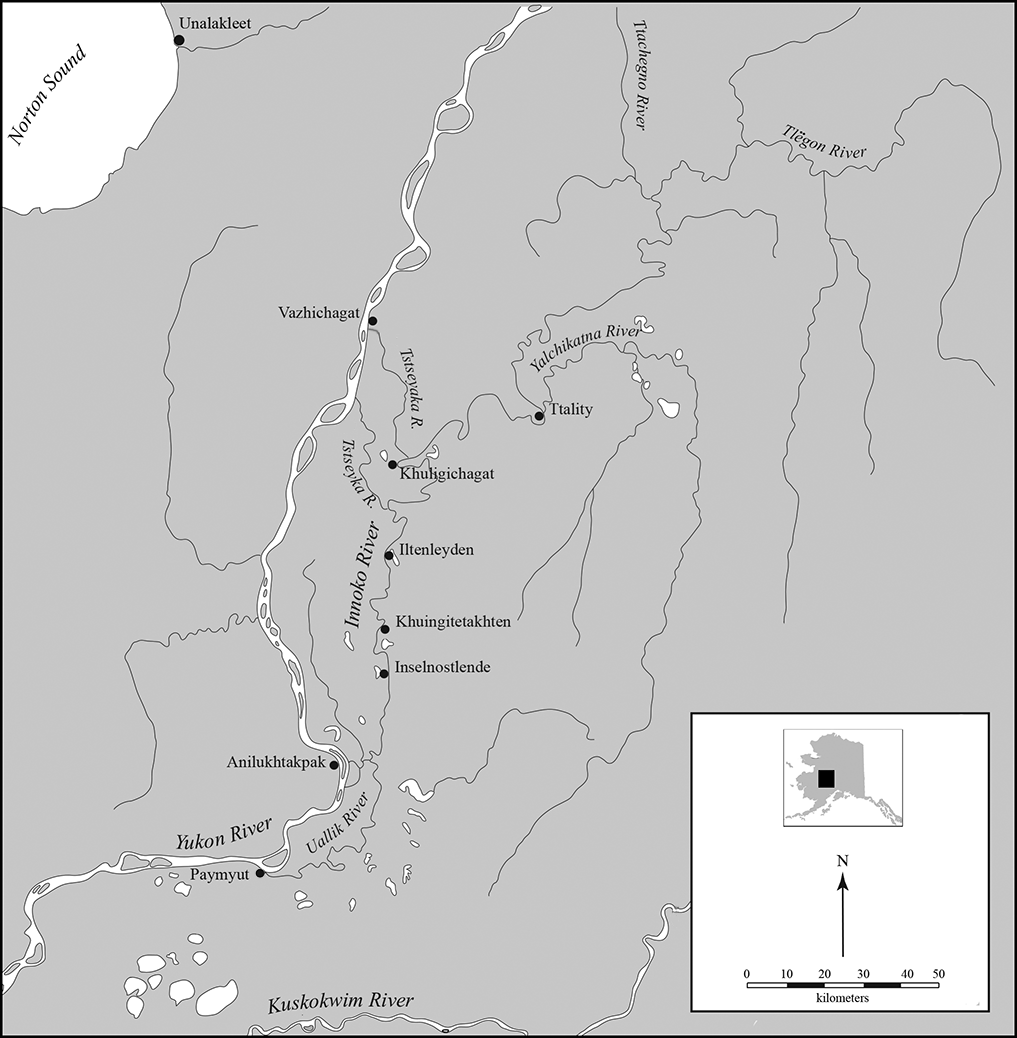
\includegraphics[width=\textwidth]{figures/pratt-fig3.png}
    \caption{Innoko River Area with Selected (Zagoskin) Place Names }
    \label{pratt-fig3}
\end{figure}

\clearpage
\begin{figure}[h]
    \centering
    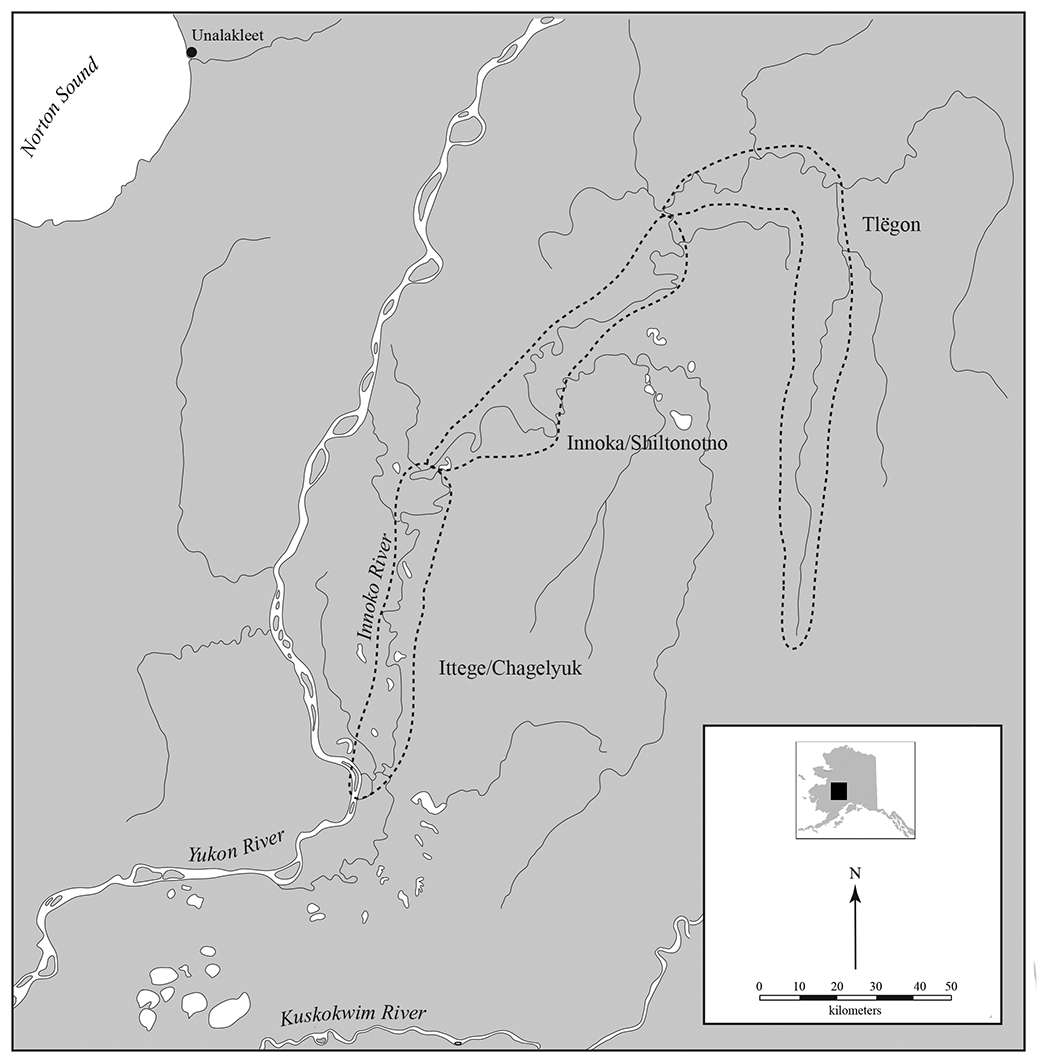
\includegraphics[width=\textwidth]{figures/pratt-fig4.png}
    \caption{Three Named Sections of the Innoko River Drainage Reported by Zagoskin}
    \label{pratt-fig4}
\end{figure}

\clearpage
\begin{figure}[h]
    \centering
    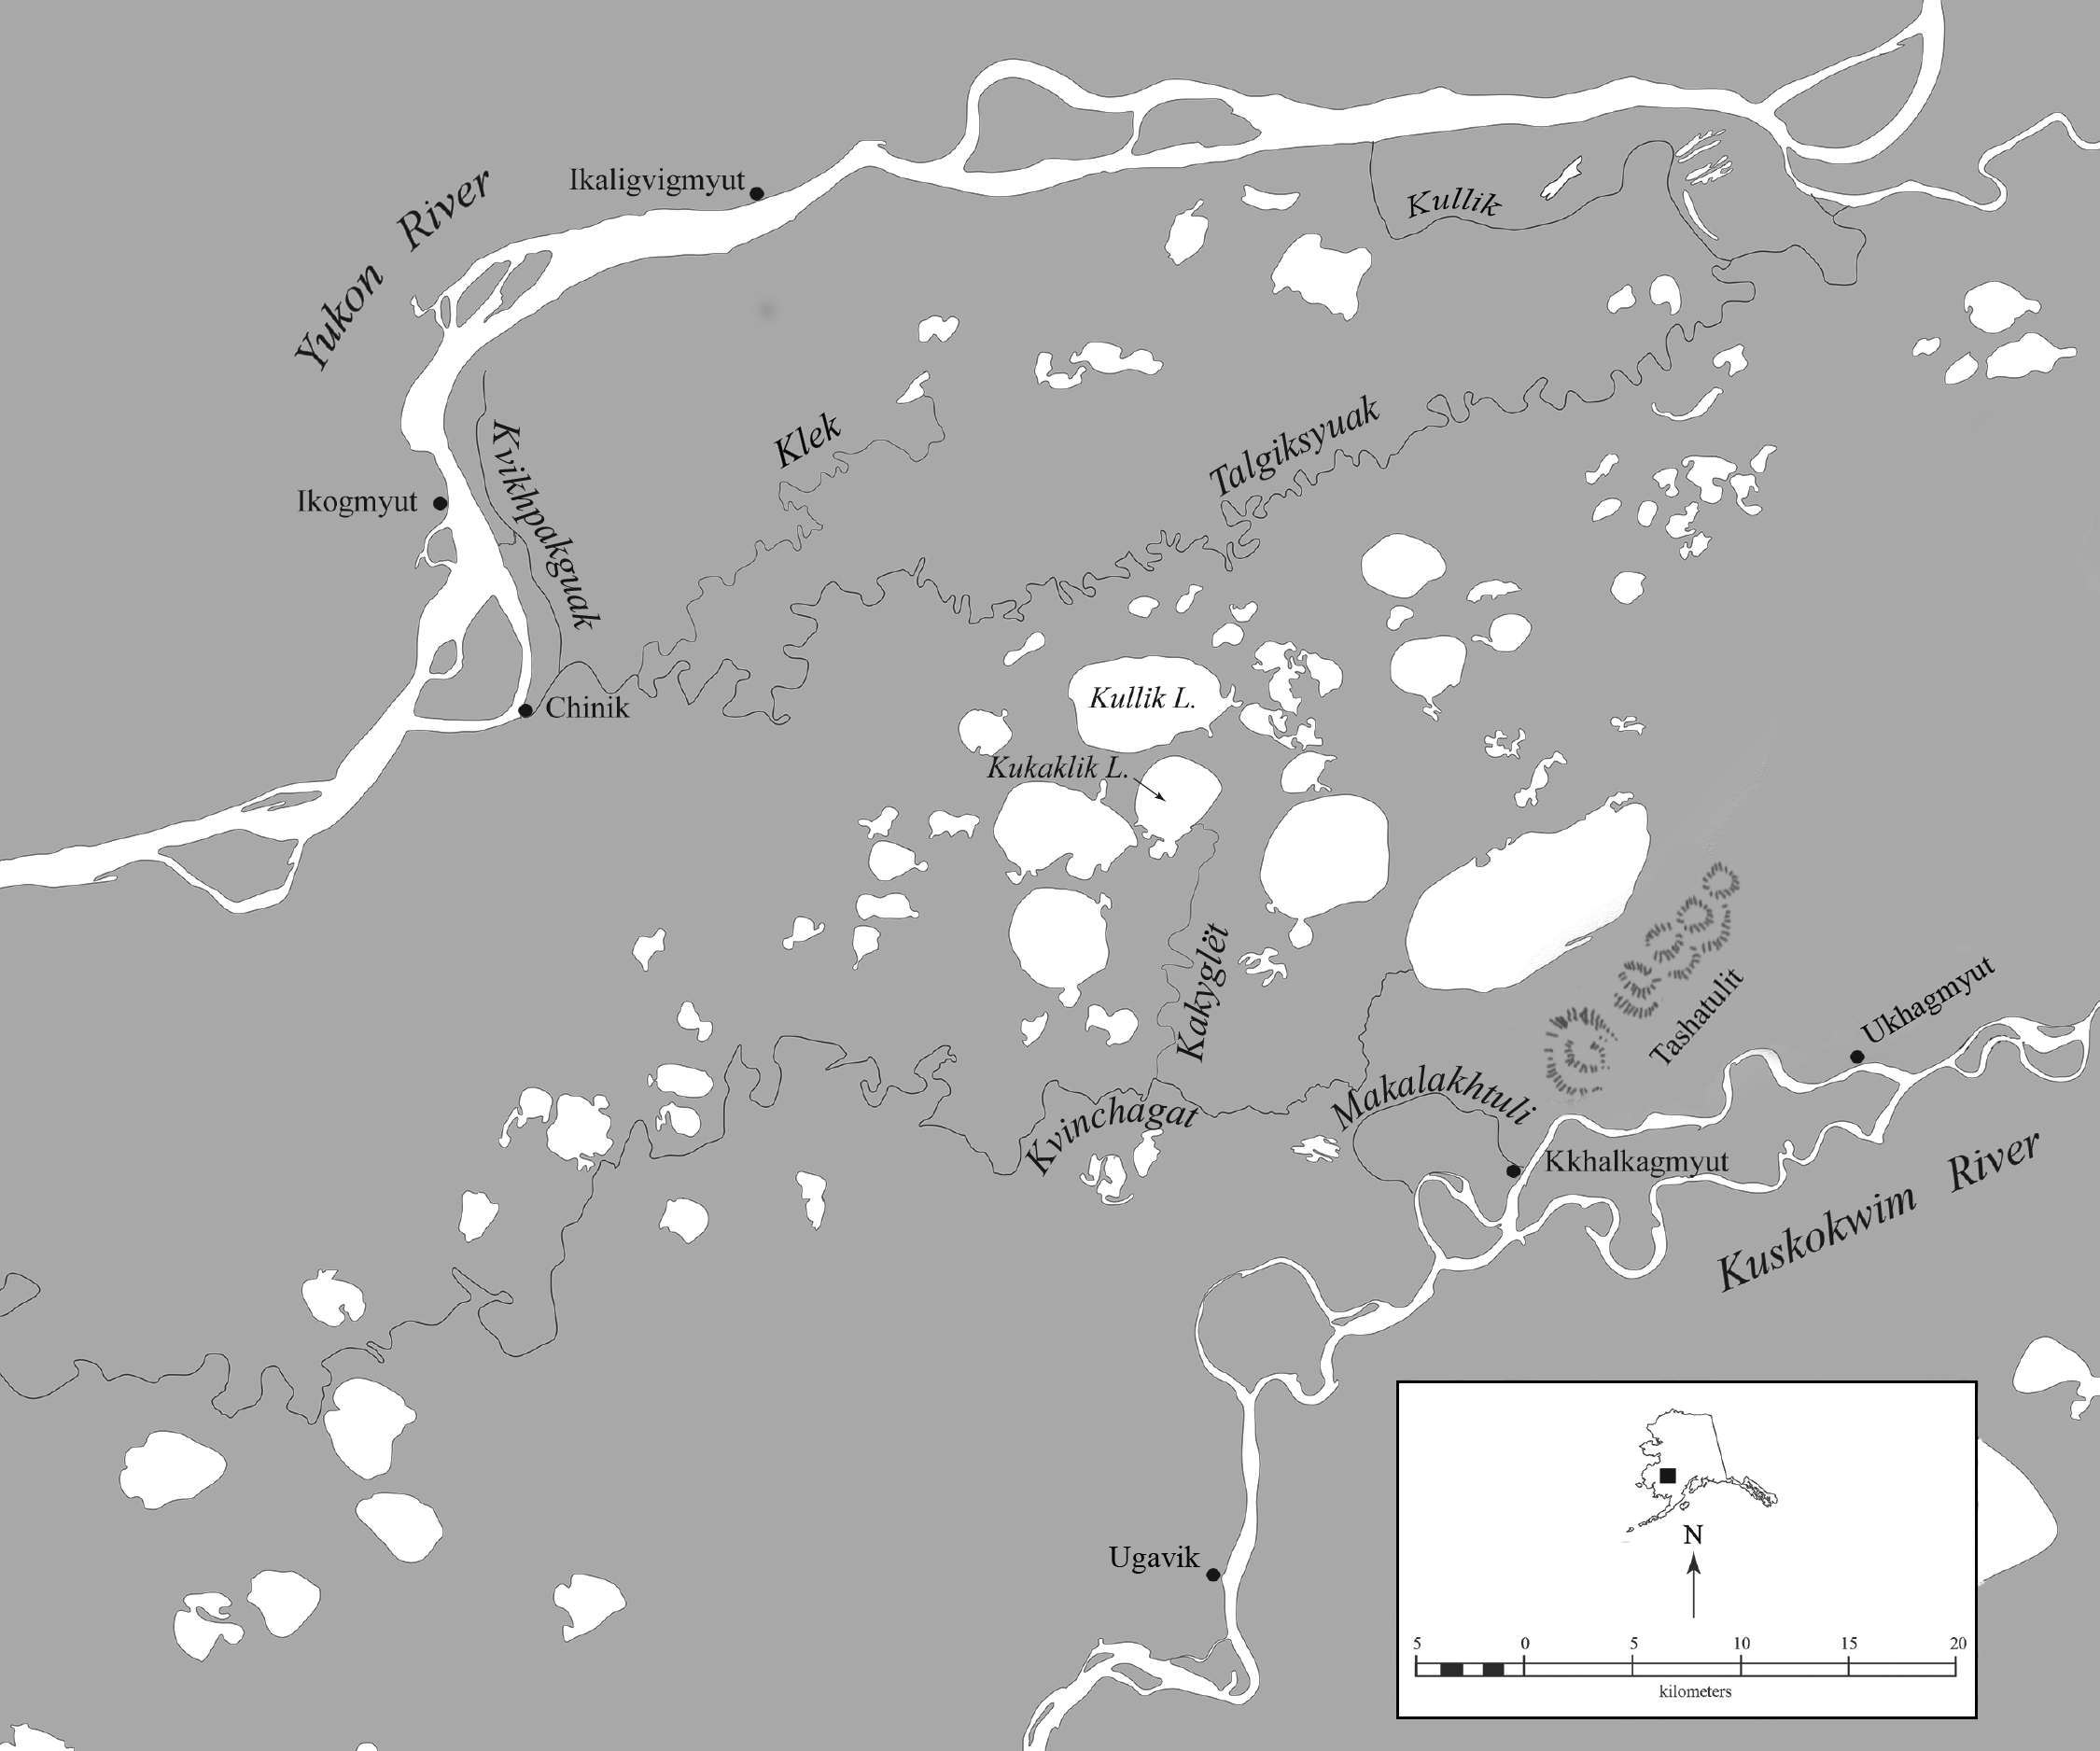
\includegraphics[width=\textwidth]{figures/pratt-fig5.png}
\caption{Yukon-Kuskokwim Portage Area with Selected Place Names Reported by Zagoskin. Map by Dale C. Slaughter.}
\label{pratt-fig5}[h]
\end{figure}

\clearpage
\begin{figure}[h]
    \centering
    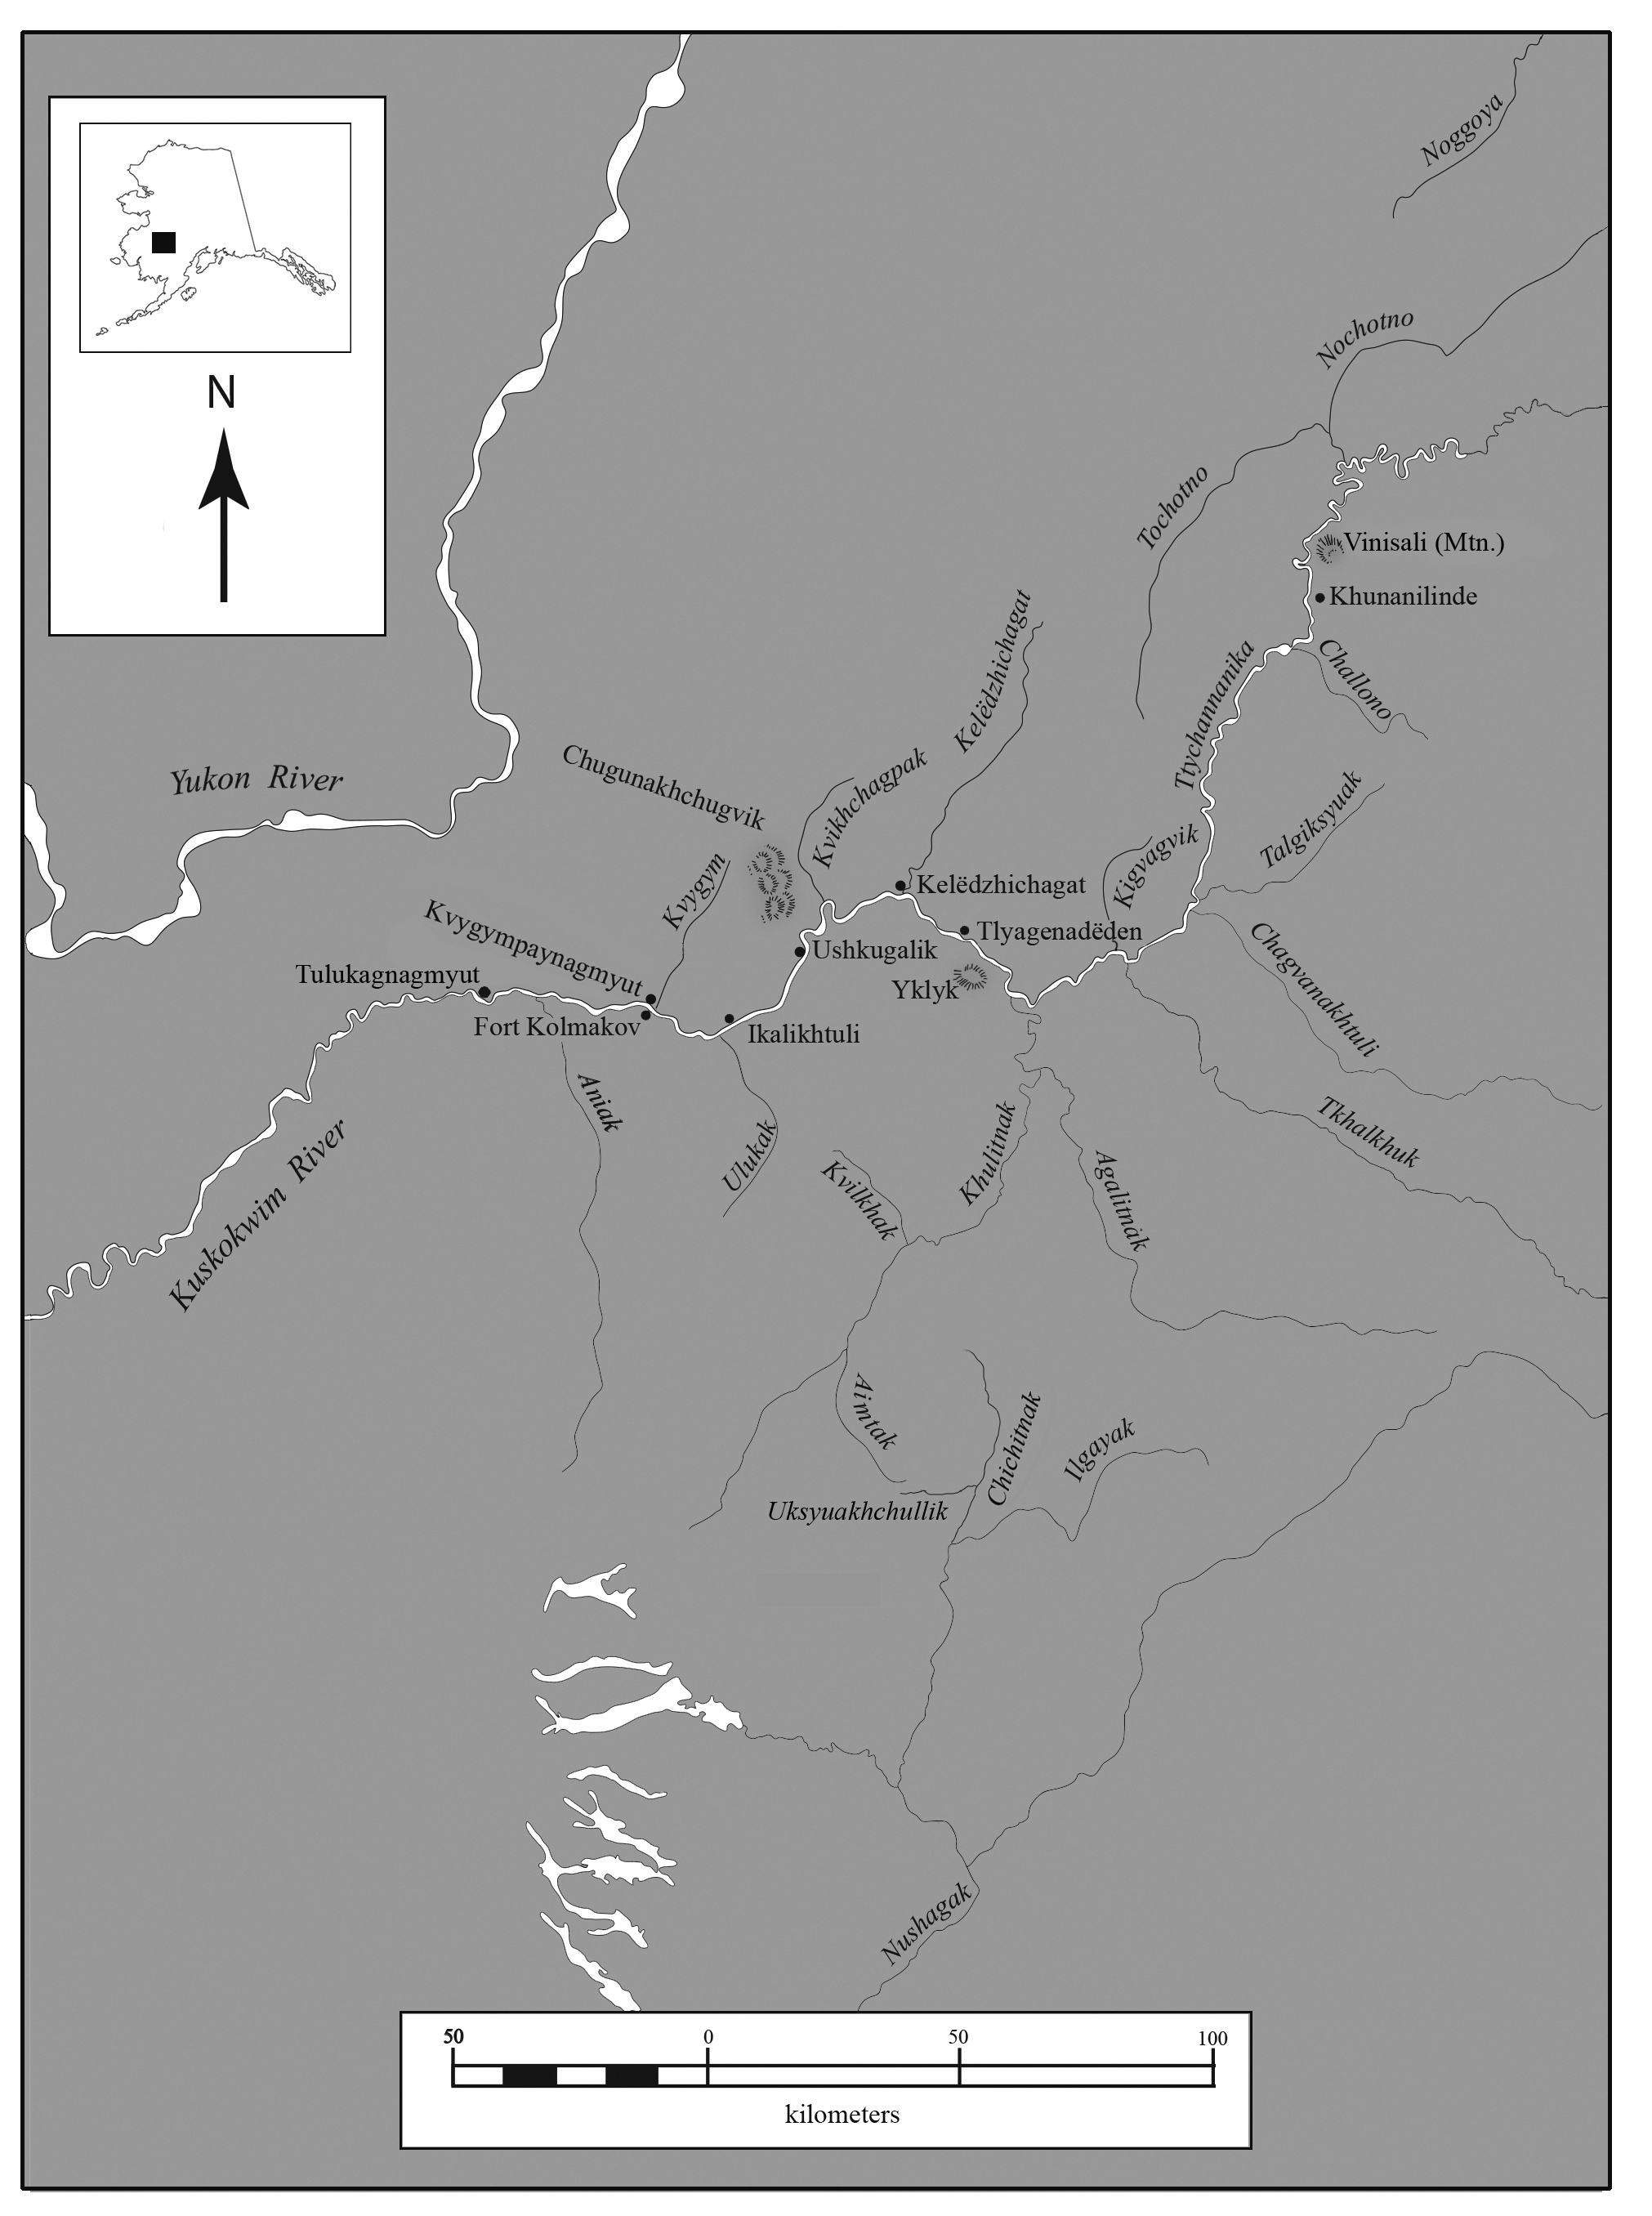
\includegraphics[width=\textwidth]{figures/pratt-fig6.png}
\caption{Middle Kuskokwim River Area with Selected Place Names Reported by Zagoskin. Map by Dale C. Slaughter.}
\label{pratt-fig6}
\end{figure}

%%%%%%%%%%%%% end appendix %%%%%%%%%%%%%%%%%%%%%







\label{pratt-ch-end}


     \chapter[Raven’s Work in Tlingit Ethno-geography]{\vspace{-25pt}Raven’s Work in Tlingit Ethno-geography}

\sethandle{10125/24840}

% \usepackage[
% 	doi=false,
% 	backend=biber,
% 	natbib=true,
% 	style=biblatex-sp-unified,
% 	citestyle=sp-authoryear-comp]{biblatex}
%\usepackage[style=ldc.bst]{biblatex}




% Author last name as it appears in the header
\def\authorlast{Thornton}

% change author in three references below to the actual author name so that this name is unique and matches the \label commands just below and at the end of the chapter
\renewcommand{\beginchapter}{\pageref{thornton-ch-begin}}
\renewcommand{\finishchapter}{\pageref{thornton-ch-end}}
\label{thornton-ch-begin}



\thispagestyle{firststyle}

\chapauth{Thomas Thornton}
\affiliation{University of Alaska Southeast}

\authortoc{Thomas Thornton}



“Raven names,” specifically geographic names by, about, and for the Raven figure of mythic time (de Laguna 1960: 129), comprise a distinct subset of toponyms in Tlingit and other Alaska Native geographic nomenclatures.  The distribution of Raven names is not random or even. Instead Raven names tend to be concentrated in areas of unique geographic abundance, dynamism, and anomaly.  Why is this so? Is it simply because of such sites conjure an elective affinity with Raven’s unique status as shaper and transformer of the world?  Or are there other factors at work?  In this paper, I explore the distribution, relations, and meanings of Raven names in Southeast Alaska and contiguous Canadian Tlingit territories within a fuller anthropological and geographical context than previously available to determine why concentrations of Raven names tend to exist where they do.  In particular I focus upon “Raven’s doings” or “Raven’s work,” as Tlingits sometimes say, as embodied in Raven names and the narratives and that accompany them.

\section{Raven’s Work}
Raven is a namer and landscape transformer in every Alaska Native and Northwest Canada First Nation oral tradition.  As the trickster-demiurge of indigenous mythology he is present at moments of dynamic change on the land, much of which is “Raven’s Work” (Yéil Dzoonáyi, see Table 1, \#20)--as one Tlingit toponym at Alsek River encapsulates—that is, a direct consequence or by-product of his ravenous dwelling.

As I have suggested in \textit{Being and Place among the Tlingit} (2008: 110), Raven is not only subject and source of names on the land, but also cultural model of the Tlingit namer. Raven perceives and negotiates many of same affordances on the land and sea as a human would, including prospects for food, water, fire, shelter, companionship to satisfy his appetites, needs, and interests, as well as hazards that may imperil him.  Yet, as an unprecedentedly endowed bird, he also has additional capacities, including bird’s eye apprehension of the world, the capacity to transform, the ability to communicate across species, and the clever wherewithal to escape danger (by wing or other means).  Many of Raven’s names show these capacities and interests, specifically. For example, Raven informs Bear of a good halibut fishing bank in an area he named “Just on the Edge of the Base of the Kelp” (Geesh K’ishuwanye), indicating both his comprehension of specific (and otherwise hidden) resource patch at the bottom of the sea, and a general principle for locating such places. In this way, Raven and his names are a model for how to apprehend and act on the world, for through his deeds and their legacies he was destined to “[show] all the Tlingit what to do for a living” (Swanton 1909: 83).

The remarkable role of Raven in Tlingit lives is emphasized by the late Lukax.ádi clan leader Austin Hammond (\textit{Daanaawáak}; see Kawaky 1981) in his own inimitable way in the film \textit{Haa Shagóon} (Our Heritage and Destiny).

\begin{quote}It was Raven who showed us how to get our food. Raven knew what was good for us, and taught the Tlingit how to live. Raven exists in our legends and in our lives. Sometimes Raven is powerful and wise, and at other times Raven seems foolish. But always the stories of Raven hold special meaning for us. It was Raven who hung by his beak suspended from the clouds at the time of the Great Flood. It was Raven who taught our people to catch salmon. These are the stories my grandfathers passed on to me. These are the things I’m trying to teach my grandchildren. It is these stories which help guide our people as we live with the land. . . . For Raven taught us, if we live with the land, not against it, the land will take care of us. The land, the river, they hear us!
\end{quote}
\noindent
As linguistic artifacts that describe, distinguish, distill the meanings of places (Thornton 2008), place names are resilient, resonant, and respected sources of Raven’s ever-vibrant relations with Tlingit country, illustrating both the wisdom of living with nature’s vitalism, and the folly of going “against nature,” which is the very definition of taboo, or \textit{ligaas’} in Tlingit (Swanton 1908; de Laguna 1972).

In what follows, I want to expand on the meaning of “Raven’s work” in Tlingit country. Specifically I want to argue that Raven is foundational to the very conceptualization of Tlingit geography because he embodies an integrative set of ideas about the indivisibility of nature/culture and its intrinsic status as: 1) formative and transformative; 2) animistic and dynamistic; 3) relational and contingent; and 4) adaptive and resilient.  As a Trickster-Transformer and world-maker, Raven is special, in his capacity to both stimulate and respond to environmental change.  Raven’s struggles with  and instigations of profound disruptions in the natural order are symptomatic of exigencies of existence in the North Pacific Rim, among the least stable and most dynamic landscapes anywhere in the world.  It is here that we find “Raven’s work.” To illustrate the significance of Raven in Tlingit toponymy, I will analyze several indigenous landscapes in the greater Southeast Alaska region with specific ties to Raven, including 1) the geography of the Great Flood in Tlingit country; and 2) the densely Raven-named and rugged Alsek River-Dry Bay region (see \hl{Map}\todo{Map?}), south of Yakutat, much of which is now part of the grand 24,312,997 acre USA-Canada Kluane/Wrangell-St. Elias/Glacier Bay/ Tatshenshini-Alsek World Heritage Site.

\begin{figure}
	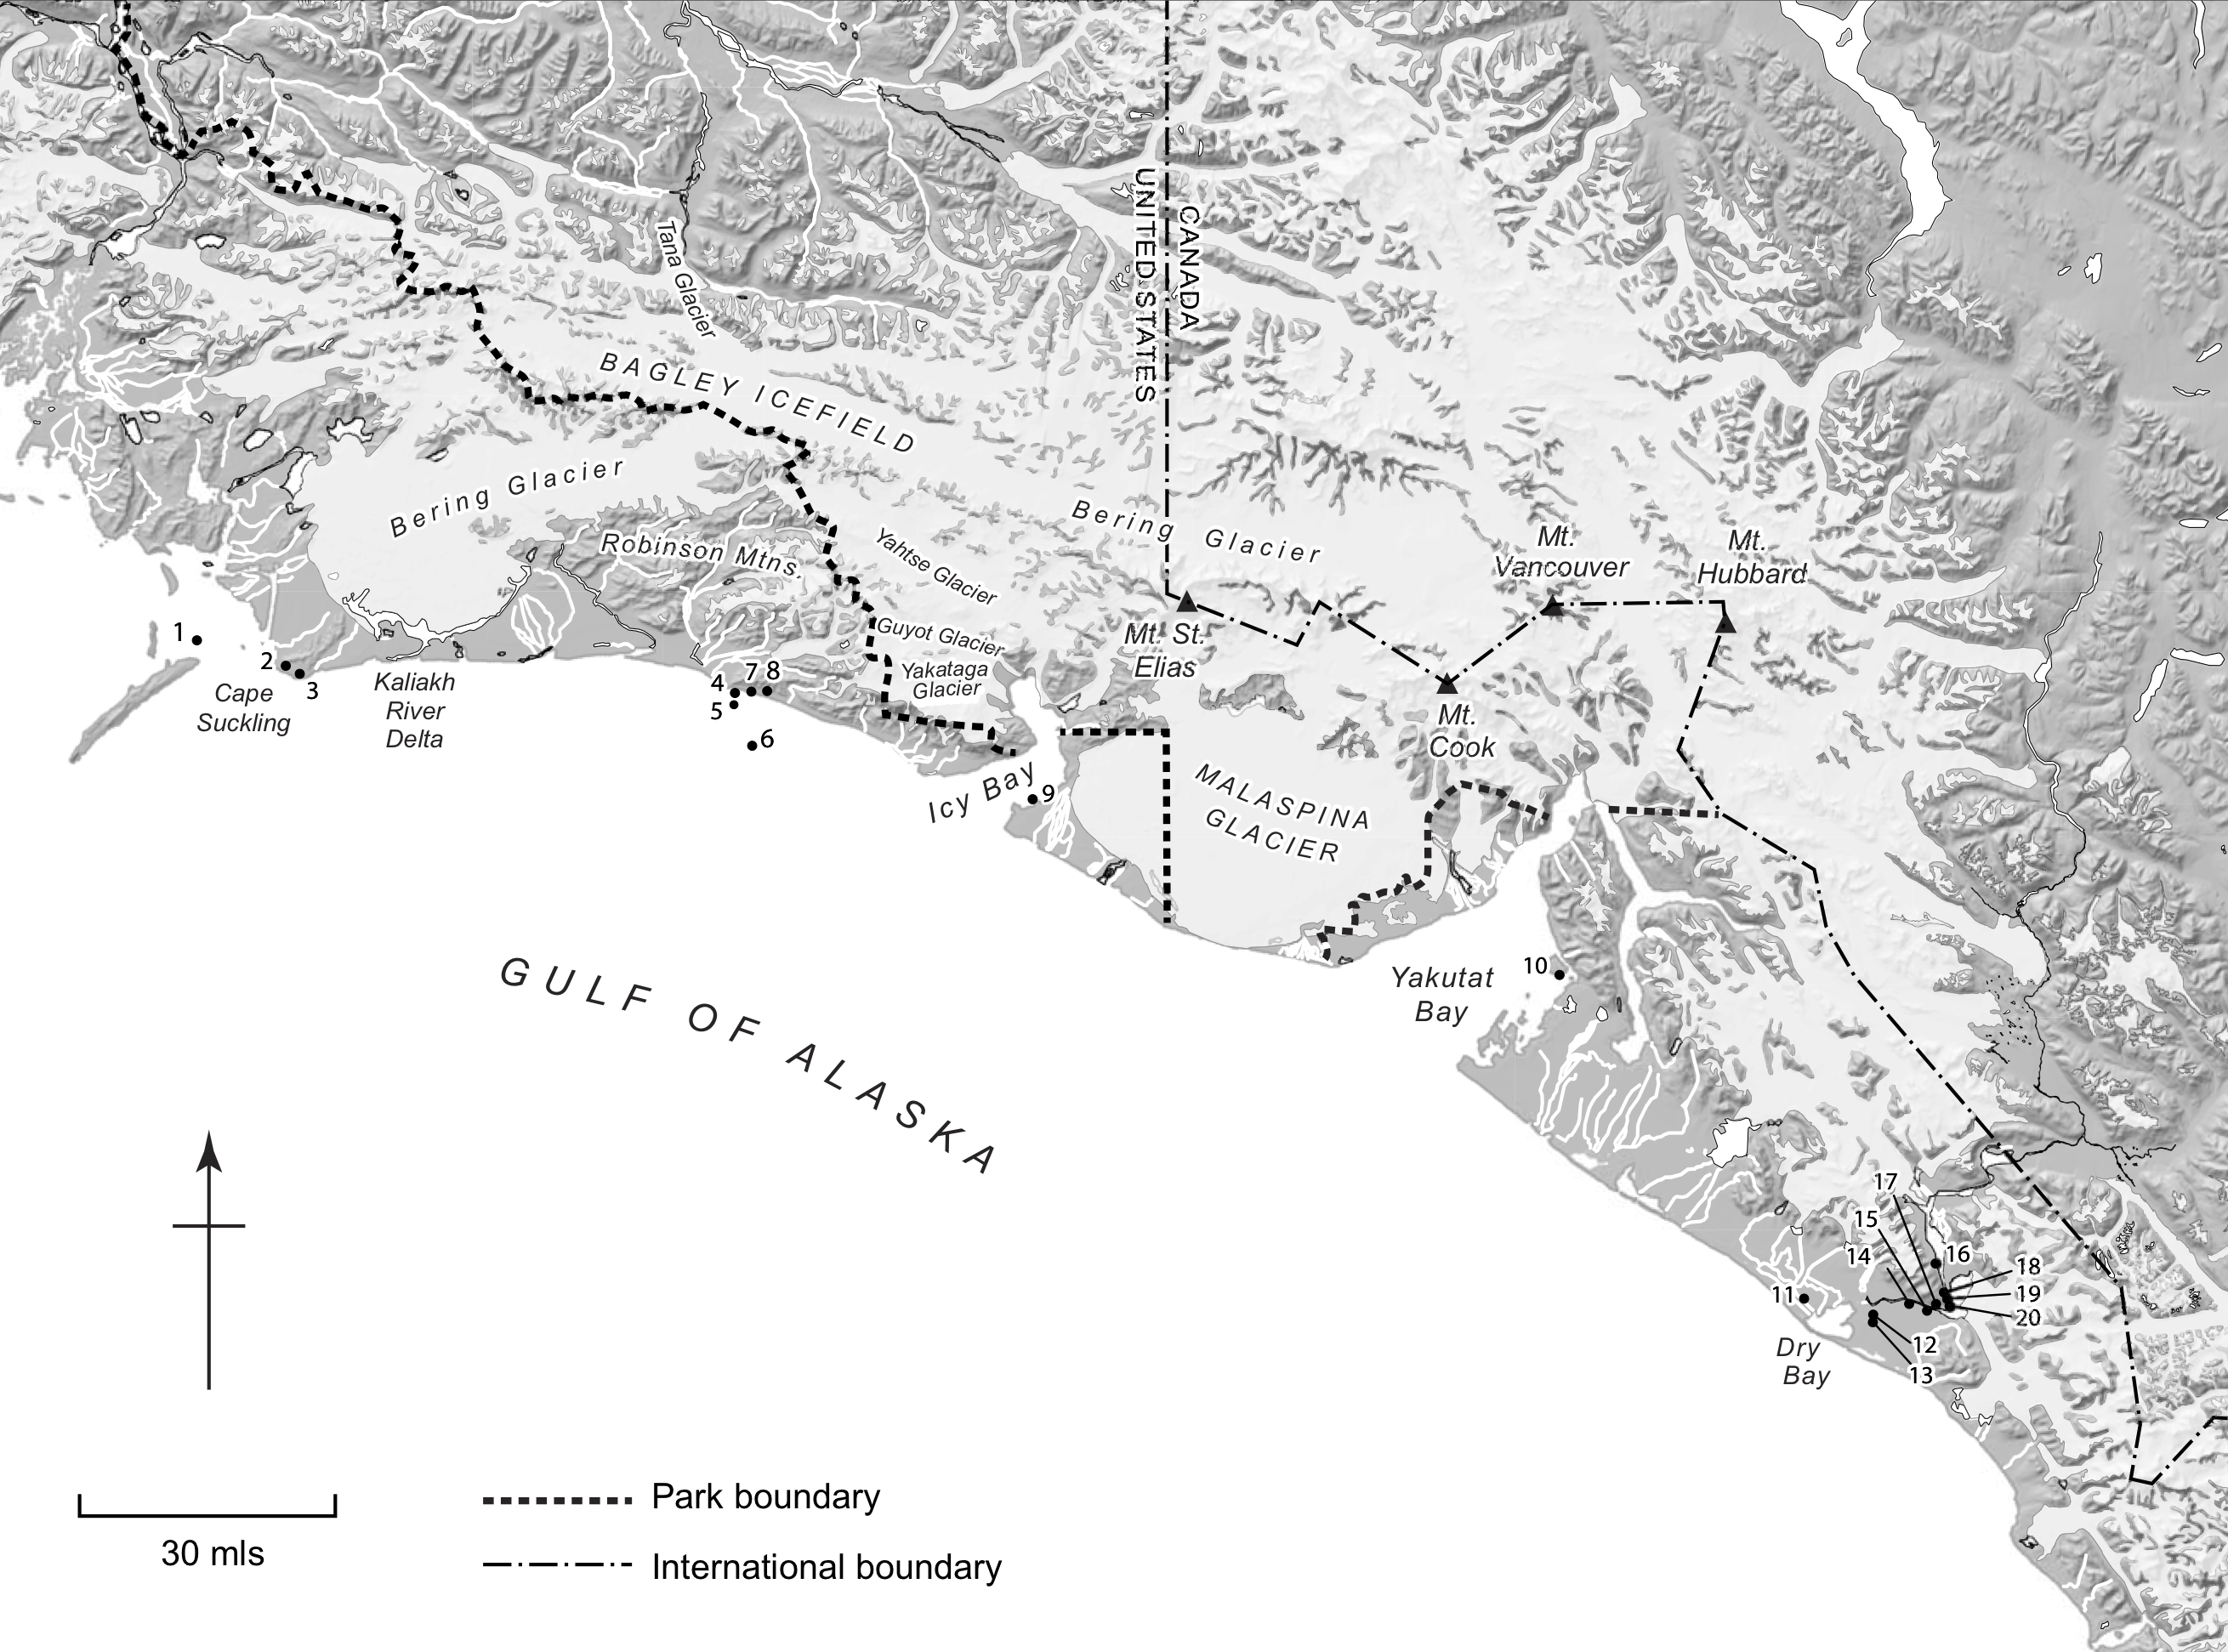
\includegraphics{figures/thornton-map1}
	\caption{\hl{map caption}}
	\label{thornton-map1}	
\end{figure}

\section{The Great Flood}
	Raven’s story begins with the Great Flood, the prototypical environmental change event, usually set at Nass River or elsewhere in Southeast Alaska.  As Chilkat elder David Katzeek tells the story, it was before the great Flood that Raven was born, to a mother who swallowed him after he transformed himself into a small, attractively smooth and shiny stone, at the suggestion of Blue Heron.  Raven was raised by his maternal uncle, who mistreats him, and their conflicts eventually trigger the Great Flood, which manifests not as torrential rainfall, as in the Bible, but rather as a great tide coming in:

\begin{quote}
    [Raven knew] that the tide is really going to come in…So the story goes that after [Raven] put his mother in [a black scoter skin] and he put her out on the water…He let it go [to float as the world flooded].  Let the tide come in.  Then the story goes ... Yéil kaawx̲a awé. Yaa aan xáas’i dei wuditeen.  I love that word [Aan xáas’i], saying that the earth has an outer skin with it way up in the atmosphere where Awu xaligaas, he [Raven] was just hanging above the earth. And nobody knows how long he hung there.  And then the story goes on to say that when the tide—when the water began to recede, was when he let go of that outer skin of the earth and fell all the way down to the waters …no one knows how many days or how long it was for him while he was falling from the outer skin of the earth, that he finally came and landed on \textit{geesh}, on bull kelp, over on this one place [perhaps near Dry Bay].  And when he sat there, up popped the sea otter.  He talked to the sea otter and he asked the sea otter, ‘Can you go all the way to the bottom?’  And that sea otter said ‘Uh huh.  Yes I can.’  ‘Well, then, if you can go all the way to the bottom, bring me some rocks and bring me some sand.’  So the sea otter goes down and brings rocks and sand to Raven.  The story goes when Raven starts throwing---he was throwing rocks out, and as he was throwing rocks all the islands started to form that are here in Alaska.  The sand that he had when he threw it out, it made the Alaska Peninsula all the way on out, the Aleutian Chain... \\

    ... But historically, the reason there are Deisheetaan from the Interior, the reason there are Killer Whales [Dak’laweidí] from the Interior, the reason there are Yanyeidis [and other clans] from the Interior … [is] because of fleeing--because of the great Flood that took place on this earth.  So that’s the story. (Katzeek 2013).
\end{quote}

\noindent
In reordering the Earth through the Flood, Raven remade the land for human habitation, exemplifying the principles of formation and transformation for which he is famous as a Transformer and world-maker. His doings thus became part of Tlingits’, indeed all Alaskan Natives’ heritage and destiny (\textit{haa shagóon} in Tlingit). In one version of the Raven cycle recorded by Swanton (1909: 81) Raven is said to have endured the Flood by turning to rock. After the Flood, it is said that:

\begin{quote}
Raven [Naas Shaak’i Yéil, Raven at the Head of the Nass River] tried to make human beings out of a rock and out of a leaf at the same time, but the rock was slow while the leaf was very quick. Therefore human beings came from the leaf. Then he showed a leaf to the human beings and said, ``You see this leaf. You are to be like it. When it falls off the branch and rots there is nothing left of it.'' That is why there is death in the world. If men had come from the rock there would be no death. Years ago people used to say when they were getting old, "We are unfortunate in not having been made from a rock. Being made from a leaf, we must die.
\end{quote}

By molding people from leaf, Raven recognised the impermanence and mutability of life on earth, the formation and transformation of its beings from seed to leaf and back again.  People may aspire to the immortality of rock (Kan 1989), but life on earth, at least for humans, is governed by change, and change defies the rigidity and permanence of rock, and rewards continued growth, evolution, and renewal of the leaf as a living, adaptive entity. It is important that people did not stand still like rocks in the aftermath of the Flood, but rather redistributed and reorganized themselves, through migration and adaptation, to the new world they faced when the waters receded.

Among the interior Tlingit and Tagish and Southern Tutchone Athapaskans the stories are similar. Elder Annie Ned described to anthropologist Julie Cruikshank (2005: 15) how “Raven, also known as Crow, originally configured the drainages from the interior to coast at the beginning of time, tipping his wings to orient them in the opposite directions; some lakes and rivers now flow north to the Yukon River and hence to the Bering Sea and other pour south to the Gulf of Alaska through the Alsek and Tatshenshini drainage.”  Thus Raven is not only the instigator of the earth-changing Flood, he is the shaper of rivers, the manipulator of tides, and in Tlingit country he is colour of the Pacific Ocean itself, which in the Gulf of Alaska at least, is simply called Yéil T'ooch, Black Raven.  This ocean, too, is Raven’s world, because it is also a result of the great Flood that Raven caused, and which he and his transformed humans had to adapt to when they returned to the coast—him from the sky and they from the mountain stone forts, where they sought refuge. The early naval Lieutenant and ethnographer George T. Emmons (1990: 82) described this mountain refuge geography thusly:

\begin{quote}
... more baffling than petroglyphs and stone carvings are cairns of piled stones to be found on mountains well above timberline, both on the mainland and on offshore islands. They have no relation to the Russian occupation, and are not boundary marks. They are away from any trails or lines of travel, at altitudes of from two to three thousand feet, located on clear stretches, generally on mountain tops. The oldest natives can give no explanation of them, beyond the story that when the great Flood covered the earth, those who survived in canoes floated up and moored their craft here with great bark ropes, the decayed ends of which it is claimed can still be seen.
\end{quote}
\noindent
These mountains “saved a lot of people” the Tlingit elders say (Jack 2013), because they afforded safety and refuge from the Flood, allowing people to survive. And after the Flood, Raven made regular tides in the ocean by manipulating the figure known as Old Woman of the Tides, who controls them, so the aboriginal people could take advantage of the sea’s intertidal bounty. These enduring geographical phenomena, including the ancestral alpine cairns and petrified remains and coastal petroglyphs and other landmarks, often marked by toponyms, remain as testimony to the adaptiveness and resilience of the aboriginal settlers in the region, and to “Raven’s work.”

\section{Raven’s Work in Northern Southeast Alaska and the Alsek River-Dry Bay System}

Between Cape Suckling and Lituya Bay in the Gulf of Alaska, Alaska’s northernmost Tlingit territory, now claimed by clans residing primarily at Yakutat, we find the highest densities of documented Raven names (Table 1).

\begin{table}[!h]
    \centering
		\small
    \begin{tabular}{l | L{3cm} | L{3cm} | L{4cm}}
\textbf{\#} & \textbf{Name} & \textbf{Translation} & \textbf{Location}  \\
\toprule

1&Yéil Xákwdli
&Raven’s Harpoon Line
&Okalee Spit \\

2
&Yéil Katsees
&Raven’s Float
&Between base of Okalee Spit and Cape Suckling \\

3
&Yéil Hít
&Raven’s House
&Cave at Cape Suckling  \\

4
&Yéil X'us.eetí
&Raven’s Footprints
&Cape Yakataga \\

5
&[Yéil ] Tayeesk'*
&Little Adze*
&Cape Yakataga  \\
6
&Yéil (Yeil) T'ooch'
&Black Raven
&Gulf of Alaska (Pacific Ocean) \\

7
&Yakwdeiyí
&Canoe Road
&Inside Cape Yakataga \\
8
&Yéil Naasa.áayi*
&Raven’s Bentwood Box*
&Cape Yakataga area  \\
9
&Geesh K'ishuwanyee
&Place below the End of the Edge of the Base of the Kelp
&Halibut fishing bank, Icy Bay \\

10
&Yéil Áa Daak Wudzigidi Yé
&Place Where Raven Fell Down
&Knight Island, Yakutat Bay \\

11
&Yéil Áx Daak Uwanugu Yé
&Where Raven Scooted Back [Kicking Up the Sand]
&Dunes on Akwe River, Dry Bay \\

12
&Kudatankahídi
&[Raven’s] Repository House
&Dry Bay \\

13&Yáay X’áat’i&Whale Island&Bear Island, Dry Bay \\

14 &Yéil Áa Yoo Akaawajiyi Yé
(Yéil Áx Daak Akawujiyi Yé) &Where Raven’s Feet Worked into the Mud Dragging (the salmon repository or “food canoe”)
&Alsek River \\

15
&Yéil Kínde Akaawatsexi Yé
&Where Raven Trampled [the Ground Packing It] Upward
&Alsek River \\

16
&Yéil Katooli Yé
(Yéilch Uwatuli Yé)
&Hole Raven Bored
&Near Gateway Knob \\

17
&Yéil Yakwdeiyí
&Raven’s Canoe Trail
&Alsek River \\

18
&Yadagwált
&Raven’s Rocks Falling Down
&Gateway Knob area \\

19
&Yéil Áa Ludaawdligoowu Yé
&Place Where Raven Wiped His Beak Off
&Alsek River \\

20
&Yéil Dzoonáyi
&Raven’s Work
&Gateway Knob \\

21
&Yei Wal'ji Héen
&Stream That Breaks Downward
&Where the Alsek River floods \\

22
&Yéil Yakwdeiyí
&Raven’s Canoe Trail
&Cape Fairweather area \\

    \end{tabular}
    \caption{Raven names}
    \label{table1}
\end{table}

The landscape with the highest densities of Raven toponyms by far is the Alsek River-Dry Bay basin, which is perhaps the region’s epicenter for change, dynamism, and Raven’s work.  Here even those toponyms that don’t reference him directly seem to be the result of Raven’s interventions. For example, Bear Island, the major island feature in Dry Bay, is known as Yáay X’áat’i (\#13) Whale Island.  But this is no simple metaphoric reference to the island’s physical resemblance to a Humpback Whale, or metonymic association to the presence of whales around the island.  Rather it is \textit{the} whale that Raven harpooned first at Kayak Island, near Cordova, with his line and float attached (\#s 1 and 2). Raven is then said to have entered the whale through its blowhole, feasted all winter on its blubbery innards, finally beaching his host at the entrance to Dry Bay, where he “wished the Whale to strand on a fine sandy beach” (and thus the Alsek delta is said to be sandy as a result; see de Laguna 1972: 84). The people that lived on the east side of Dry Bay, known as Whale’s Fat (Yáay Taayí) heard Raven calling, and, after initially being scared by the this sound, dragged the whale further ashore and flenzed it, eventually opening a hole big enough for Raven to fly away with his customary “k̲aa!” cry of Trickster triumph, having tricked the people out of some of the whale meat and fat.  Significantly, when the people at Gus'eix̲, the village at Dry Bay, faced a later Flood, caused not by Raven but a local clan’s mistreatment of a seagull, the whale’s “fin,” a marked protrusion on the island, served as a mooring for people to tie their canoes as the flood waters washed the settlement away (de Laguna 1972: 76).\footnote{Today this island, though still recognized for its origins as a whale, carries the Tlingit name Gal'jinoowú (Clam Hand Fort, though its etymology is uncertain, according to de Laguna 1972: 84), perhaps reflecting a major adaptation of the Tlingit and other Northwest Coast peoples: cultivation of clam “forts” or “gardens” (Thornton, et al. 2015), basically engineered beds to stabilize and enhance habitat for these marine invertebrates.  Perhaps such cultivation represents another of Raven’s lessons on how to subsist in a changing world.  Unfortunately, the oral history does not tell us.  }

Raven’s food quest is also evident in his tracks on the west side of Dry Bay, which are produced after he drags in the famous “ark” or food canoe and builds a repository house (\#12, Kudatankahídi), sometimes referred to as Raven’s Party House, variously located at Dry Bay, Cape Yakataga or Cape Suckling.  The food canoe, which in fact also supported kelp-bed edifice to house marine creatures, was heavy and the effort to drag it arduous, these efforts being marked by the place names Yéil Áx̲ Daak̲ Uwanugu Yé (\#11), Where Raven Scooted Back [Kicking Up the Sand] and Yéil Áa Yoo Akaawajiyi Yé  (\#14) or, Yéil Áx̲ Daak̲ Akawujiyi Yé), (Where Raven’s Feet Worked into the Mud Dragging).  According to Yakutat elder Fred White (2001), who spent time with his grandparents at Dry Bay, you can see Raven’s tracks at the sand dunes between Ustay and Akwe rivers, the dunes themselves having resulted from when Raven dragged the canoe to shore, working his feet into the mud, and kicking up sand.  Like Noah’s ark, this great canoe was said to house all the animals we find in the world today.  As de Laguna recorded:

\begin{quote}
    At the Dry Bay (eastern) end of the long, narrow island between these two sloughs, there is a sand dune. On this I was told could still be seen the footprints made when Raven with a cane shaped like a devilfish tentacle drew ashore an ``ark'' filled with all kinds of food animals. Canoe Prow House of the [L’uknax̲.ádi clan] refers to the enclosed prow of this canoe, and the [L’uknax.ádi] use a dance paddle shaped like the cane. The point, 'Atuqka [?] [Evidently the “fin” used to moor the canoes in the abovementioned flood], was "a place just like the prow of a canoe...”
\end{quote}

Bert Adams (1998), a L’uknax̲.ádi clan elder, adds: “When he pulled the ark ashore, the birds were released and that is why we have birds in the world today.  As he pulled the ark from the ocean he left his foot prints in the sand hills along the Akwe River and that is where Gus'eix̲ [village] is. This goes along with the story that the Lukaax̲.ádi [another clan] people were the earliest people in the Dry Bay area and initially built their house in Gus'eix̲. When the L’uknx̲x.ádi people came from southeast they eventually took over Gus'eix̲ and probably changed the name to Digginna hit [Deikinaa Hít], Far Out House.”

Bert Adams, Fred White and others (see de Laguna 1972), also agree it was at Alsek River-Dry Bay where Raven opened The Box of Daylight he stole form his grandfather at Nass River (de Laguna 1972: 84), and in doing so, not only released the sun, the moon and the stars into the cosmos, but frightened everything else—even the rocks and the mountains---off the face of the land from Dry Bay up to Ocean Cape, leaving only sandy forelands.

\begin{quote}
Raven also lured ashore the first king salmon in Dry Bay. The mountain down which Raven was thrown in a box, is above the Akwe River. Near the second glacier ascending the Alsek, Raven threw away his wife's basket and a big king salmon. The cave, or house of stone [Yéil Ta Hít?], in which Raven lived is southeast of Lituya Bay; it is [in] the mountain he slashed [Yéil Nées' Akawlishaa, Raven Ate Sea Urchin, perhaps Mount Crillon or Mount La Pérouse] when angry at Echo [for imitating his loud slurping sounds, eating sea urchins (see also de Laguna 1972: 93)].  In this area, Raven obtained the first plants and trees from the Sea Otters [after the Great Flood, referenced above]. There is also another of his landing places near Cape Fairweather or Lituya Bay. It is in this area where we can see how the surface of the land was shaped in primordial time (Adams 1998).
\end{quote}
\noindent
Thus, Raven’s Alsek River-Dry Bay landscape is not only the source of all creatures in the world, but the source of the world itself, and the place where the entire planetary system was released to support life on earth.

Animism and dynamism in the land are reflected in the Alsek River itself, and its major tributary, the Tatshenshini, which were both said to possess powerful spirits and animate geographic features and constituted lucrative trade routes and perilous passages. Trade routes linked the coast and Interior Tlingit and Athabaskan communities, and also lead to the wealthy Chilkat and Chilkoot Tlingit tribes at Haines (Deishu, End of the Trail) and Klukwan (Tlákw.aan, Eternal Village) (De Laguna 1972; Thornton 2011, 2012). Deieenaak’w, The Sitka elder who recorded much Tlingit oral history for Swanton in 1904 (Swanton 1909), emphasized the living spirit and animistic qualities of the glaciers in this area: “In one place Alsek River runs under a glacier. People can pass beneath in their canoes, but, if anyone speaks while they are under it, the glacier comes down on them. They say that in those [early] times, this glacier was like animal and could hear what was said to it.” The dangers, including recurring ice bridges, blockages, and flooding are well catalogued by Natives and non-Natives alike (see de Laguna 1972: 87), and summarized by Cruikshank (2005: 236; see also de Laguna 1972: 885-90):

\begin{quote}
Danger points reported by all river travelers were two canyons, each formed by a rock wall facing an actively calving glacier (see conventional 9). At the first, about 30 kilometres upriver from the mouth, an expanded Alsek Glacier formed a vertical wall of ice some sixty metres high, stretching for more than six kilometres and interrupted only by “Gateway Knob,” a tall nunatak or promontory from which rocks the size of golf balls rained down. It was here that an ice bridge formed periodically.  Sometimes a lake, subject to outbursts [i.e., flooding], formed just below. Tlingit narrators attributed Gateway Knob’s formation to the travelling world-maker, Raven, who distributed geophysical features at the beginning of time. They commented on Raven’s wife’s dismay whenever she passed beneath this knob’s jutting rock face, lest she be killed, and Raven’s modest reassurances that rocks would not touch the boat unless some passenger was fated to die.
\end{quote}

"That's where the rocks fall all around,” one of de Laguna’s (1972: 87) informants remarked, “and they call it Yel tsunayI [Yéil Dzoonáyi, Raven's Work]. When my father was going up to Tinx kayani [Tínx Kayaaní, Bearberry/Kinnikinnick Leaves, near Sediment Creek on the Tatshenshini River], it [the golf ball sized rocks] touched his boat. That same summer they drowned."  Even today, more than an half century after de Laguna’s last major fieldwork, these stories still resonate, enlivening the landscape and enlightening people as to how to engage its potency.  These rules of engagement, entailed by Raven’s instigations, but evolving through subsequent relations with human and other-than-human beings remain relevant and contingent for success in adaptation and resilience in this dynamic, ever-changing landscape. Thus, songs and sayings people recited as they passed vulnerably under the Alsek’s ice bridges, active glaciers, and shedding rock walls-- Yéil Dzoonáyi— are remembered and performed at potlaches and other appropriate contexts, rendering Raven’s work and its entailing events as sacred \textit{shagóon} or chronotopes,, places in a community’s geography where time and space are forever fused as sacred heritage and destiny (see Bakhtin, cited in Thornton 2008: 17).

\section{Conclusion: The Resonance of Raven Landscapes from the Pleistocene to the Anthropocene}

Raven names form not only a genre of geographic nomenclature but mark exceptional, dynamic and anomalous environments throughout Tlingit country and beyond.  I have focused particularly on well documented Raven geographies in mythic time (the Great Flood) and the contemporary late Holocene in northern Southeast Alaska.  While I have highlighted the dynamic far northern Dry Bay-Alsek River frontiers of the Tlingit settlement, other unique and potent parts of their territory exhibit similarly evocative Raven names and evidence of his “work” on the land,  if not in the same rich concentration: Kootznahoo Inlet inside Angoon, with its strong reversing tidal falls (Yéil Eeyí ,Raven’s Tidal Current), Keku Straits and Saginaw Bay areas near Kake (e.g., Yéil G̲áachk'u, Raven’s Little Mat, a flat-topped island landmark in the Keku Islands where Raven laid a mat of plants, and Yéil Kawóot, Raven’s Beads, a unique limestone bed of fossil crinoids that Raven once used to fashion a necklace for his wife); Peril Straits above Sitka with its narrow passes and forceful currents (e.g., Yéilch Wóoshdáx̲ Wulixidi Yé, Place where Raven Broke Through, by creating a passage with his paddle); and Upper Lynn Canal near Haines with its dramatic mountain canyons and rocky shores (e.g., Yéil Háatl'i, Raven’s Excrement, a rocky shore near Battery Point, below Haines, or Yéil Áx' Sh Wulg̲eig̲i Yé, Place Where Raven Swung, in a mountain valley) (see Thornton 2012).

As the legends recount, Raven had to steal the various elements that comprise the world—the earth, the moon, the stars, freshwater, fire--and, after enlightening and enlivening the world, he embarked on his quest to gather together those resources necessary to sustain a life: freshwater, wood and other materials for fire and manufacture, medicines, and various foods. His descendants still pursue this quest and follow the trails he has inscribed in the landscape. People hunt, fish, and gather in the vicinity of X’as’tuhéen ([Raven’s] Driblet Creek, in Excursion Inlet, Near Hoonah), created by the drops that spilled from Raven’s mouth as he flew away from Petrel after stealing the latter’s spring water (at Hazy Islands, southwest of Kuiu Island); collect intertidal resources at Skanáx (Noisy Beach, in Saginaw Bay, where Raven found the squirting bivalves cacophonous); land their boats at Yéil Kiji Yakwdeiyí (Raven’s Wings Boat Road, on the Khaz Peninsula, near Sitka), where he quieted the sea to create a smooth trail amid the rocks and swells so he could safely land his canoe; and net fish in the vicinity of Yéil G̲eiwú (Raven’s Web or Fishnet, at Gut Bay, a premier sockeye salmon stream on Eastern Baranof Island used by primarily by Kake Tlingits), now petrified in stone above the tide line, the webbing still visible (de Laguna 1960). These are just a few of the ways that Raven’s work continues to shape peoples understandings and responses to the land throughout Tlingit country.

Given his special association with unique, dynamic and transforming landscapes, it is no accident that so many of Raven’s acts in Tlingit country can be traced, in one form or another, to the greater Dry Bay-Alsek River area.  This landscape is one of the richest and most remarkable anywhere in the world in terms of its topographic and microclimatic variation, active tectonic, glacial and fluvial processes, abundance of fish, wildlife and edible plants, as well as sheer grandeur.  From the standpoint of human being making a living, it also has all of the affordances (see Thornton 2011) to sustain and endanger life in all of its vicissitudes and vitality. At the same time, this landscape constitutes a palimpsest or meshwork (Ingold 2000) of lines of intersection, interrelation, and interanimation among its constituent beings and the forces that have shaped their dwelling over the longue durée.  Among the lines of intersection are the “hydronymic districts”---a concept coined by Jim Kari in his pioneering studies of Athabaskan place names---which manifest in the lower and middle Alsek and Tatshenshini rivers between Athabaskan and Tlingit toponyms.  Other lines relate prehistory to present history, interior-coast trade, travel, and migration, and animate relations between people, land and sea.  Raven is foundational to all these connections and we would be wise to promote further understanding of his toponymic districts and their associations to better understand, value, and conserve this World Heritage site.  For it was here that Raven formed and transformed the land itself, spawned earth’s systems by opening the Box of Daylight, and showed the people how to navigate and negotiate the exigencies of life, to make their living with nature, not against it, and to adapt and survive in this complex, ever-changing world.

In the end, then, Raven names embody all that this Trickster-Transformer-Worldmaker has represented from his mythic beginnings: a set of powerful, contingent, collaborative and conflicting appetites and forces that make physical and social existence possible but also a continuous drama and struggle. In this sense, as I have argued elsewhere, Raven’s unruly foibles and inscriptions on the land constitute a good model for how to understand not only the Pleistocene and the Holocene, but also what contemporary scientists have termed “The Anthropocene,” a new geologic epoch in which human activities are now impacting most profoundly on the very earth systems that we rely on to sustain us (cf. Crutzen and Stoermer 2000; Thornton and Thornton 2015).  Pessimistic prognosticators see a great reckoning ahead in this new epoch, payback for the havoc humans have wreaked on the planet in the industrial age, while optimists see opportunities for humans to embrace their dominance and engineer a better world.  Raven reminds us that both visions are flawed, and anthropocentric.  The Great Flood, darkness, famine, and other disasters have all been visited on earth before, with many winners and losers, but the people survived, rock-like on the mountain tops. And when the topography and ecology changed, they adapted, flexibly and resiliently, renewing themselves, like leaves.  At the same time, as Raven also shows us, hubris and the aspiration to engineer the earth to our selfish ends have always been with us. But for us, as for Raven, things rarely work out as planned, and when we insult or push earth systems too far (as in the Tlingit concept of taboo, \textit{ligaas’}, “against nature”), there are often unanticipated consequences: other living beings, including the rocks, the waters, and the glaciers, may push back, putting humans in jeopardy.  Thus, humility, awareness and attentiveness to earth systems and other-than-human beings, and, finally, preparation for change and contingency are in order if we are to survive the Anthropocene.  This is but one of many lessons implicit in Raven’s integrated toponymy and topography at Dry Bay-Alsek River and elsewhere in Alaska and beyond, where we find Raven’s work. Before there was the Anthropocene there was the “Ravencene,” and it was bigger, more dramatic, and more all-encompassing than its new anthropocentric counterpart. More importantly, it will always be with us in one form or another.


\refheading

\begin{hang}
Adams, Bert. 1998. Interview and Stories of Dry Bay, Alaska, Project Jukebox, University of Alaska, Fairbanks. Accessed August 2015. \url{http://jukebox.uaf.edu/drybay/htm/stories.htm}

Cruikshank, Julie. 2005. \textit{Do Glaciers Listen? Local Knowledge, Colonial Encounters and Social Imagination}. Vancouver: University of British Columbia Press.

Crutzen, Paul J. \& Eugene F. Stoermer.  2000. The Anthropocene. \textit{Global Change Newsletter} 41. 17–18.

De Laguna, Frederica. 1960. \textit{The Story of a Tlingit Community: A Problem in the Relationship between Archeological, Ethnological, and Historical Methods}. Bureau of American Ethnology, Bulletin 172. Washington DC: US Government Printing Office.

De Laguna, Frederica. 1972. \textit{Under Mount Saint Elias: The History and Culture of the Yakutat Tlingit}. 3 vols. Washington, DC: Smithsonian Institution Press.

Ingold, Tim . 2000. \textit{The Perception of the Environment: Essays in Livelihood, Dwelling, and Skill}. London: Routledge.

Jack, Mabel. 2013.  Interview with Thomas F. Thornton for Alpine Cairn project, National Science Foundation. Angoon, Alaska, July 24. Transcript in Thornton’s possession.

Kan, Sergei. 1989. \textit{Symbolic Immortality: The Tlingit Potlatch of the Nineteenth Century}. Washington, DC: Smithsonian Institution Press.

Kari, James. 1987. Some Principles of Alaska Athabaskan Toponymic Knowledge. In Mary R. Key \& Henry Koenigswald (eds.), \textit{General and Amerindian Ethnolinguistics: In Remembrance of Stanley Newman}, 129–49. Berlin: Mouton de Gruyter.

Kari, James. 1996. A Preliminary View of Hydronymic Districts in Northern Athabaskan Prehistory. \textit{Names}  44(4). 253-71.

Katzeek, David. 2013. Interview with Thomas F. Thornton for Alpine Cairn project, National Science Foundation. Juneau, Alaska, July 22.

Kawaky, Joseph (producer). 1981. \textit{Haa Shagóon}. Film presented by Chilkoot Indian Association. Juneau, AK: Sealaska Heritage Foundation

Swanton, John R. 1908. Tlingit.  \todo{incomplete reference?}

Swanton, John R.. 1909. \textit{Tlingit Myths and Texts}. Bureau of American Ethnology, Bulletin 39. Washington, DC: Government Printing Office.

Thornton, Thomas F.   2008.	\textit{Being and Place among the Tlingit}.  Seattle: University of Washington Press.

Thornton, Thomas F. 2011.  Language and landscape among the Tlingit. In   David M. Mark, Andrew G. Turk, Niclas Burenhult \& David Stea (eds.), \textit{Landscape in Language: Transdisciplinary Perspectives}, 275-89. Amsterdam and Philadelphia: John Benjamins Publishing.

Thornton, Thomas F. (ed.). 2012.	\textit{Haa Léelk'w Has Aaní Saax'ú: Our Grandparents’ Names on the Land}. Seattle and Juneau: University of Washington Press and Sealaska Heritage Institute.

Thornton, Thomas F., Douglas Deur \& Herman Kitka Sr. 2015. Cultivation of Salmon and Other Marine Resources on the Northwest Coast of North America. \textit{Human Ecology} 43(2). 189-199.

Thornton, Thomas F. \& Patricia M. Thornton. 2015. The Mutable, the Mythical, and the Managerial: Raven Narratives and the Anthropocene. \textit{Environment and Society: Advances in Research} 6(1). 66-86.

White, Fred. 2001. Interview on Dry Bay, Alaska, Project Jukebox, University of Alaska, Fairbanks. Accessed August 2014. \url{http://jukebox.uaf.edu/drybay/htm/tape10.htm}

\end{hang}


\orcidfooter{Thomas Thornton}{tthornto@alaska.edu}{}
\label{thornton-ch-end}


     \chapter[T'aak̲ú Téix̲'i - The Heart of the Taku]{\vspace{-25pt}T'aak̲ú Téix̲'i - The Heart of the Taku:
A multifaceted place name from the Taku River Tlingit First Nation
}

\sethandle{10125/24841}

% \usepackage[
% 	doi=false,
% 	backend=biber,
% 	natbib=true,
% 	style=biblatex-sp-unified,
% 	citestyle=sp-authoryear-comp]{biblatex}
%\usepackage[style=ldc.bst]{biblatex}




% Author last name as it appears in the header
\def\authorlast{Schreyer}

% change author in three references below to the actual author name so that this name is unique and matches the \label commands just below and at the end of the chapter
\renewcommand{\beginchapter}{\pageref{schreyer-ch-begin}}
\renewcommand{\finishchapter}{\pageref{schreyer-ch-end}}
\label{schreyer-ch-begin}



\thispagestyle{firststyle}

\chapauth{Christine Schreyer}
\affiliation{University of British Columbia, Okanagan Campus}

\authortoc{Christine Schreyer}

\section{Introduction}

The traditional territory of the Taku River Tlingit First Nation stretches across northwestern British Columbia into the Yukon and Alaska and encompasses the watershed for which the community is named –the Taku River. This paper examines the multi-faceted use of one place name from the locale of the Taku River, an island known as T'aak̲ú Téix̲'i or the Heart of the Taku. This name serves multiple roles within the community. It is a border marker, but it is also a central point or the “heart” of the community’s territory. The name and a series of metaphors associated with it are also used to invoke principles of stewardship and protection of the land, or what I have referred to as “performatives of stewardship” (Schreyer 2016). The specific locale, T'aak̲ú Téix̲'i, can also be examined using Thornton’s (2011) model for understanding ecotopes, which he describes as the “smallest ecologically-distinct landscape features” (Hunn and Meilleur 2010: 15ff), which hold cultural significance (Thornton 2011: 276).

The island T'aak̲ú Téix̲'i is found on the Alaskan side of the international border between British Columbia and Alaska, but as Louise Gordon states, “the Elders and our ancestors always believed that the rivers, the watersheds, are the borderlines. They didn’t say borderlines, but for them it was the rivers [that were important]” (Gordon L., interview 2006). Kari’s extensive research on Athabaskan place names, as described these mapping systems based on drainage systems as “hydronymic districts” (Kari 1996a). For example, in their research on Tlingit and Haida Land Rights and Use, Goldschmidt and Haas documented that:

\begin{quote}
The original home of the Taku people was on the Taku River. After the establishment of the international boundary, the Taku Tlingits split into two groups, one living upstream on the shores of Lake Atlin, and the other remaining on the coast. The two groups still recognized their unity and maintained contact (Goldschmidt et al 1998: 41).
\end{quote}

As well, despite this imposition of the boundary, the members of the Taku River Tlingit First Nation still use the river on both sides of the border and know the land there intimately. \ Thornton writes, “Many Tlingit place-names are evocative of the mythical and historic past, in so far as they serve to cement the traditional relationship between a particular group or clan and the territory that continues to sustain them” (2008: 102). As will be explained below, the place name T'aak̲ú Téix̲'i or the Heart of the Taku comes from a mythohistoric story about how the landscape of the Taku River was formed, and, therefore, it is one place that illustrates the long-lasting and sustaining connection community members have with the Taku River. Recently, however, the use of the toponym has also been extended to include another locale, a BC Parks Conservancy called the Taku River/T’akú Téix’ Conservancy.\footnote{Consistency in spelling remains a challenge for this community where very few Elders are fluent in Tlingit and none of the Elders have ever been schooled in Tlingit literacy. For this reasons, and others that will be noted below, spelling of the name T'aak̲ú Téix̲'i is inconsistent. } In many colonial nations, place names that are layered on top of one another create a stratigraphy of history (Schreyer 2014) where settler names sit on top of indigenous names. While this is also true in Taku River Tlingit territory (Schreyer et al. 2014), in this specific example, the community has chosen to extend a well-known and important place name laterally, to a different terrain and for a new purpose, and in this manner the place name T'aak̲ú Téix̲'i has become even more tied to stewardship since it is used for a conservancy to protect the land.

Prior to this use of the Tlingit name, T'aak̲ú Téix̲'i, as a form of stewardship, imbricated English metaphors tied to the Heart of the Taku have also been used by community members to assert their stewardship over their lands and in their traditional territory. Following ideas from Mac Cormac on the role of metaphors as performatives, as well as Thornton (2012, 2011, 2008) on metaphor and anatomical connection in Tlingit place-naming practices and the concept of ecotopes, I trace the use of the Heart of the Taku from Mrs. Nyman’s telling of the place name’s origin (Nyman and Leer 1993) to how the name and the ideas associated with the name are used in contemporary times (2014).

\section{Background on the Taku River Tlingit First Nation}

Originally designated by the government of Canada as the Atlin Band, after the large lake (Áa Tlein in Tlingit) on the shores of which their government offices are now located, the Tlingits of northwestern British Columbia began to self-identify to outsiders as people of the Taku River in the early 1980s in association with the start of land claims negotiations in the community. As Alice Carlick told me in an interview from my doctoral research, “a lot of us didn’t like [the name Atlin Band] because we are matrilineal and we do come from the Taku River” (Carlick, A., interview 2006). The Taku River has long been a locality of great importance for the Taku River Tlingit in terms of culture, including economics, politics, social cohesion, and healing. Therefore, the community continues to assert their stewardship over their lands, and this river, in many ways. For instance, in 1999, the Taku River Tlingit First Nation began working with the Round River Organization, a conservation group, in order to develop a sustainable land plan, also known as the Conservation Area Design, to further strengthen their argument for stewardship over their lands and to support their court-case against the mining company, Redfern Resources, that wanted to build a road through the heart of their traditional territory. This case was heard at the Supreme Court of Canada in 2004 and, although the Taku River Tlingit First Nation lost the case on an appeal, their case set legal precedence on issues of consultation. In 2003, the community published the beginnings of a land plan (the Conservation Area Design and a Vision and Management Document).

Since 2003, the Lands and Resources department has released other documents that illustrate their stewardship of their lands. These include the Taku River Tlingit First Nation Mining Policy (2007); the map of the Taku River Tlingit Tlatsini or ‘The Lands That Keep Us Strong’ (2009); and Wóoshtin wudidaa - Atlin Taku Land Use Plan (2011). The Wóoshtin wudidaa - Atlin Taku Land Use Plan is a unique and historic example of government-to-government negotiations that was signed by the province of British Columbia and the Taku River Tlingit First Nation, which according to one news source “balances stewardship with development” (ICTMN 2011). Both the Vision and Management Documents (2003) and the Wóoshtin wudidaa - Atlin Taku Land Use Plan include statements that support the use of Tlingit language, and Tlingit place names in particular. This is important to note since Tlingit is not the everyday language of the community members and very few fluent speakers of the language remain in the community (TRTFN-ALI 2014).

Therefore, while some people do know the Tlingit name of T'aak̲ú Téix̲'i (Heart of the Taku), this name is also used in a variety of different ways in English as well, as I describe below. In addition, since there is a desire in the community for language revitalization, the community members have developed various programs and projects to help encourage more Tlingit language use. Among these is the development of an interactive, participatory map, which records Tlingit place names, the English meaning of the Tlingit place names, audio recordings of Elders saying the place name, and finally, photos of the place. This website was developed through a joint research project between the Taku River Tlingit First Nation and researchers at the University of British Columbia, including myself, in order to: 1) support Tlingit language revitalization and 2) illustrate the community’s continued stewardship over their lands. I describe this website in more detail below, but first turn to the origins of the name T'aak̲ú Téix̲'i and the Heart of the Taku.

\section{Remembering the Giants’ Battle}

One of the first published records of the Heart of the Taku comes from Mrs. Elizabeth Nyman, a respected Taku River Tlingit Elder who passed away in 1999. Mrs. Nyman co-authored the book \textit{Gágiwduł.àt: Brought Forth to Reconfirm - The Legacy of a Taku River Tlingit Clan}\footnote{ For the publication of this book, Jeff Leer developed an alternate Tlingit writing system that was used in Atlin until recently, which continues to be used in some areas of the Yukon. In 2006, the Taku River Tlingit Elders Council voted to start using the orthography popularized by Sealaska Heritage Institute. Therefore, in this article all Tlingit writing is in this orthography, often known as the Coastal Orthography. Quotes from Mrs. Nyman’s book, however, retain their original spelling.}  with linguist Jeff Leer (Nyman and Leer 1993). In this book, the transcription of the story entitled “The Battle of the Giants” appears in the both Tlingit and English. This story, which Mrs. Nyman told in 1988 in Tlingit, describes the mythohistoric battle that two giants (Was’as’ê and Łkùdasêts’k) engage in over the Taku River. Eventually, Was’as’ê rips Łkùdasêts’k apart and throws pieces of his body all over the Taku. He declares, “Let Łkùdasêts’k’s heart become the Heart of the Taku” (Nyman and Leer 1993: 5), and to this day that heart, the island, remains in the Taku River. The story of the T'aak̲ú Téix̲'i also appears in Mrs. Nyman’s telling of “T’aakhu Yan Yédì Dat Shalnik” or the history of the Taku Yanyeidí\footnote{Yanyeidí is the clan name spelled in the Sealaska orthography and will be the spelling used when not referring to a specific item from the Nyman and Leer (1993) book. } clan, which she recorded in 1984. Yanyeidí is the wolf clan of the wolf moiety to which Mrs. Nyman belonged.\footnote{ Yán is the Tlingit word for Western Hemlock (Crippen 2010), which is what the clan’s house was built of on the Taku River. It also appears in the name of the mountain K’iyán (Hemlock grows around the bottom).} Throughout this story, Mrs. Nyman again describes the giant’s battle because it is significant to the history of the Yanyeidí people who built their clan houses on the Taku River. In this story Mrs. Nyman describes in more detail what the pieces of Łkùdasêts’k look like when he is ripped apart and where they landed, including his head (which is also an island), and his windpipe (on a mountain), which has water so cold flowing from it that no one can drink it. About his heart, she says:

\begin{quote}
His heart he yanked out and threw it into the Taku River. There is a small island there, perhaps a little larger than this room, stretched out so; only short grass grows on it. “This will be the Heart of the Taku”, said Was’as’ê....This is what my father-in- law used to tell us, since he was a young boy they told him that it’s still the same as ever. For some reason it never drifts away, the Heart of the Taku? I suppose it is still there to this day. [Nyman and Leer 1993: 29]
\end{quote}

I have been working with the Taku River Tlingit First Nation since February of 2005 on issues relating to language and land, including place names and their importance (Schreyer et al 2014). However, I have never heard this story told; I have only read Mrs. Nyman’s version. This is not to say that community members do not know the story and the significance of T'aak̲ú Téix̲'i\textbf{. }For instance, Elder Jackie Williams, Mrs. Nyman’s oldest son, mentions this island in his story about the forging of the peace treaty and border between the Taku River Tlingit and their Tahltan neighbors to the south. In one section of the story, he describes the Heart of the Taku as a border marker between inland and costal Tlingit people. He says, “\textit{T’aakú Téix’i} marks the limit to which the ocean backs the river water up during high tide, and so is a marker of the boundary between the Taku Tlingit and the \textit{Éil’ ká ku.oowu Lingít }(“salt water people” or coastal Tlingit people)” (Williams 2013). As well, in an interview that I conducted with Louise Gordon, she described the Heart of the Taku as being a place that is of special importance to her and the community as a whole. She said:

\begin{quote}
Down the Taku there’s an island and it’s kind of shaped like a heart and they call it “The Heart of the Taku”, and [the elders] believe that if that island goes away or if someday it will erode then the Taku will not be the same. [Knowledge] like that is probably most important to us. [Gordon interview 2006]
\end{quote}

This knowledge is part of the reason, why the Taku River Tlingit First Nation has worked so hard to protect their land, and specifically, the Taku River.

\section{Locating the Heart}

As described above, T'aak̲ú Téix̲'i and the Heart of the Taku became a central point of focus when the Taku River was jeopardized by a major development in the early 1990s. Redfern Resources, a mining company, wanted to build a road through the community’s territory, which, if constructed, would have caused a huge impact on an otherwise undeveloped large portion of their territory and would have disrupted their traditional way of life. A community made film from this time period states that Redfern Resources wanted to:

\begin{quote}
Re-open a base-metal mine on the east bank of the Tulsequah River, near the Alaska border. The Tulsequah’s glacial waters empty into the Taku...the mine’s reopening [would have cost] more than \$140 million, and \$33 million of which would have gone to construct a 160-kilometre-long, all season road through \textit{the heart} of the TRTFN’s traditional territory.\footnote{Tulsequah is an anglicized spelling and pronunciation of the Tlingit name Taaltsux̲éi, which means root garden. This place was the site of a Tlingit village (see \url{trt.geolive.ca}). } [Taku 1997: 1-2, emphasis added]
\end{quote}

This first battle with mining companies over the river ended in 2004 when the community lost their court case against Redfern on an appeal to the Supreme Court of Canada (SCC 2004 74). More recently, however, the community has filed another lawsuit to protect their river, against Chieftain Metals Inc., which has replaced Redfern Resources as the mining company operating the Tulsequah Chief Mine on the Taku River. The current issue is that the province of British Columbia renewed the certificate of the mine without consulting with the First Nation, as legally required (Rivers Without Borders 2014). On July 24\textsuperscript{th}, 2014, a verdict on this suit was rendered; “The Honourable Justice George Macintosh has ruled that the BC government breached its duty to consult the Taku River Tlingit First Nation when making a critical determination regarding the Tulsequah Chief Mine” (Ecojustice 2014). Since this announcement last summer, the British Columbia Ministry of Environment has determined that the Tulsequah Chief Mine project has been substantially started and the company is therefore permitted to continue the development of the mine (Canadian Press 2014).

However, in both court cases, the community and their supporters make reference to the Taku River as being the “heart” of Taku River Tlingit Territory. For example, the Rivers Without Borders media release on the recent court case states, “The proposed Tulsequah Chief mine is in the \textit{heart} of the Taku River Tlingit’s traditional territory on the banks of the Tulsequah River, a major tributary to the Taku River, and just upstream of the Alaska/BC border” (RWB 2014, emphasis added). While the phrase “the heart of the territory” calls to mind the English synonym for “the center of the territory”, community members often understand this to have a polysemic or double meaning, which includes reference to the English version of the island’s name. The island, the Heart of the Taku, then is iconic of the whole of the river. For example, when I met Terry Jack, a Taku River Tlingit fisherman, for the first time in the summer of 2006 I explained that I was researching the connection between language and land for Taku River Tlingit community members and the first thing he asked me was, “But, you’ve never been down river? You’ve never been to the Heart of the Taku?”\textsuperscript{ }(Schreyer field notes 2006). The double question about down river (an often used phrase to refer to the Taku river) immediately followed by “the Heart of the Taku”, is an excellent example of this extended use of the meaning that has moved from the Tlingit place name T'aak̲ú Téix̲'i to the English translation Heart of the Taku, and then to the extended English meaning of “center”. Not only has the name itself been extended with a new linguistic meaning, but it has also been extended on the land. In particular, the name has also come to be a form of social action and stewardship is in the recent development of a BC Parks Conservancy called the Taku River/T’akú Téix’ Conservancy. Established on June 22\textsuperscript{nd}, 2012, the BC Parks website provides the following information about how this area developed:

\begin{quote}
Taku River/T’akú Téix’ Conservancy was established as a result of the Wóoshtin Wudidaa Atlin Taku Land Use Plan and Taku River Tlingit First Nation Strategic Engagement Agreement. \\

This conservancy encompasses the BC portion of the Taku River main stem from the Alaska border to the confluence of the Nakina and Inklin Rivers. The Taku River Tlingit First Nation has a deep and significant cultural attachment to the Taku River, reflecting a long history of use, occupation and spiritual connection. The Tlingit name (T’akú Téix’) means “Heart of the Taku”. The conservancy is located approximately 65 kilometers south of Atlin.\footnote{ Nakina is an anglicized spelling and pronunciation of the Tlingit place name Naak’ina.áa Héeni (the lower Nakina River from the confluence with the King Salmon River, known as T’á Héen in Tlingit), which was named for an old village in this area. Inklin is an anglicized spelling and pronunciation of Héen Tlein, meaning “big river” in Tlingit (see: trt.geolive.ca). } (\url{http://www.env.gov.bc.ca/bcparks/explore/cnsrvncy/taku-rv/})
\end{quote}

A significant point from this description is that this conservancy is located within the Canadian side of the Taku River, despite the fact that the original T'aak̲ú Téix̲'i is located on the Alaskan side. T'aak̲ú Téix̲'i and the English, Heart of the Taku, therefore, have numerous and extended meanings within this community.

As Kari has written about the general symbolic Athabaskan geography, “The place names appear in networks and constitute cognitive maps. The place names/signs have had several functions – to facilitate memorizability, and way-finding, to mark travel corridors, to represent land use agreements, or to mark band boundaries” (1996b: 464).\footnote{ I am honored to be included in this volume dedicated to the work of James Kari. His thorough examination of Athabaskan place names has long been an inspiration for my own work. } This can be seen to be true for this Tlingit place name, which is a key locale in a highly significant travel corridor for Taku River Tlingit people. The name is also used to represent contemporary and past land agreements and to mark the boundary between inland and coastal Tlingit peoples. Beyond this an interesting and different set of extended meanings have developed in this community, which are tied to the origins of the Tlingit place name T'aak̲ú Téix̲'i. According to Mrs. Nyman’s story, the island T'aak̲ú Téix̲'i is Łkùdasêts’k’s heart and a set of metaphors related to this anatomical organ are also found in use amongst Taku River Tlingit community members in English.

\section{Of Hearts and Blood}

Within a booklet that was co-written by the Taku River Tlingit First Nation and BC Wild (a conservation group) in support of the Taku River Tlingit First Nation’s first court case, examples of this extended set of metaphors are present. This booklet (see Figure1), printed in 1997, is entitled, “Taku: Will a short-lived mining project sever the \textit{bloodline }of the Tlingit people?” (1997: cover, emphasis added).

\begin{figure}
    \centering
    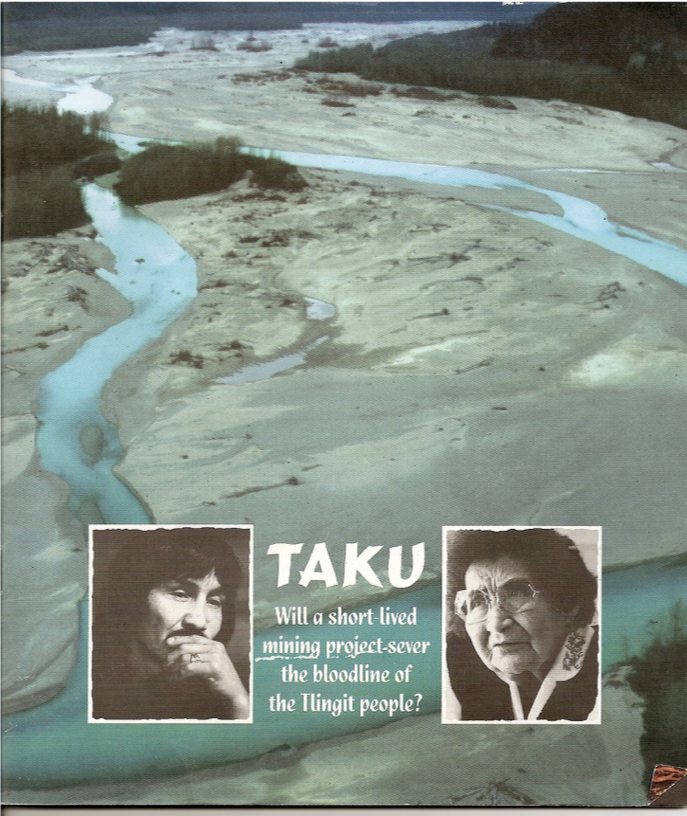
\includegraphics{figures/schreyer-fig1}
    \caption[width=0.5\textwidth]{Taku pamphlet (1997) – the many veins of the Taku River. Bryan Jack, Crow Director (left), and Antonia Jack, Crow Elder (right), are shown as well.}
    \label{schreyer-fig1}
\end{figure}




Similar to the polysemic meanings that the term “heart” holds, the word “bloodline” has multiple meanings in this context for Taku River Tlingit community members as well. English speakers may first think of veins or arteries and the connection to the heart, but veins are also used to describe rivers. The Taku River has many different veins (as seen in Figure 1), but importantly the veins of this river or the bloodlines are those that connect to the Heart of the Taku, to the island. As well, bloodlines in English may also cause English speakers to think of their familial relations. In this case, as Tlingit communities are matrilineal, bloodlines are tied to clans and clans are tied to places. Thornton describes clans as “oldest and most basic unit of Tlingit social structure and the foundation of both individual and group identity” (2008: 46-7), and he goes on to discuss the relationship between clan and place in his book \textit{Being and Place among the Tlingit.} He writes:

\begin{quote}
The linguistic homology between clan and place leads to other metaphoric associations, too. Two images are especially poignant: place/clan as protector and place/clan as provider...in a metaphor of sustenance, the Tsaagweidí can allude to their connection with the key resource, harbor seal (tsaa), found in their place of origin, Hood Bay (Tsaagwáa, “Seal Ice Floes”). Such metaphors are skillfully blended in the context of visual and verbal art. [Thornton 2008: 54]
\end{quote}

The Heart of the Taku is a key place in the history of the T'aak̲ú K̲wáan; the island and the river help to sustain the whole community, but it is of particular importance for community members from the Yanyeidí clan, specifically, whose clan houses were originally built on the Taku (Thornton 2012; Goldschmidt et al 1998).

However, within the text of this booklet, yet another meaning is provided for bloodlines. The Taku River Tlingit First Nation fisheries manager from 1997, Cecil Anderson, describes “the Taku’s salmon as the Tlingit’s \textit{bloodline}” (1997: 8, emphasis added). Fish are hugely important to both the economy of the community and the subsistence of community members. For instance, the salmon from the Taku River is sold by the community-owned and run company, Taku Wild, which sells smoked salmon from the Taku River around the world. The profits from this company support conservation efforts and land planning. On their website it is written, “Our home is this land. Our spirits, lives, and hearts have been shaped here, and we will care for our land just as our ancestors have instructed us” (Taku Wild 2014).

As well, the Taku River Tlingit First Nation currently practice what is known as “food fishing” or the community fishing by Taku River Tlingit members for the rest of the community living in Atlin and Whitehorse. A variety of salmon species are found in the Taku River, including Sockeye, Coho, and Chinook each year (TRTFN 1997), and these are all distributed throughout the community by the fisheries department. I have been in the community when the fish is distributed, and it is always an exciting time! People try to get their favorite type of fish; families join together to share and process the fish, which always arrives whole. The fish is filleted and special parts are laid aside: the head, the fins, and tails (see Figure 2). Due to Atlin’s isolation (it is a 2 hour drive from Whitehorse, Yukon down a windy gravel road), store bought food can often be more expensive than in the city and perishable items often spoil quickly. The salmon then are a healthy source of food, but there is also a spiritual or emotional connection to food that comes from the land. Even in the Taku River Tlingit’s constitution (1993), it is written, “It is the land from which we come that connects all life. Our land is our \textit{lifeblood}” (as quoted in TRTFN 2003, emphasis added). Terry Jack, a Taku fisherman mentioned earlier, is quoted in the Lands and Resources Vision and Management Document - Hà t\_tátgi hà khustìyxh - Our Land is Our Future (2003), his feelings on the salmon that feeds the community:

\begin{quote}
The fish to our people is one of our \textit{lifelines.} And not only that it’s so sacred to our people. It’s a food that represents us as Tlingits...when I think of Taku fish, I think of it as coming from the \textit{heart of the Tlingit country}. [TRTFN 2003: 60, emphasis added]
\end{quote}
\noindent
An interesting chain of word associations can be seen as the following:

\begin{center}
$ \textbf{Bloodline} \longleftrightarrow  \textbf{Lifeblood} \longleftrightarrow \textbf{Lifeline}$
\end{center}

All of these words connect the salmon to the land, but also suggest the other connections to the heart, arterial veins, the veins of the Taku River, and ties to matrilineal clan. \\

Since 2006, some of the fish from the Taku fishery’s harvest has been given to the community’s dance group, the T'aak̲ú K̲wáan Dancers, in order that they can put on a Salmon Barbecue and raise funds to travel to Juneau, Alaska to participate in Sealaska Heritage Institute’s Celebration (see Figure~\ref{schreyer-fig1}).

\begin{figure}
    \centering
    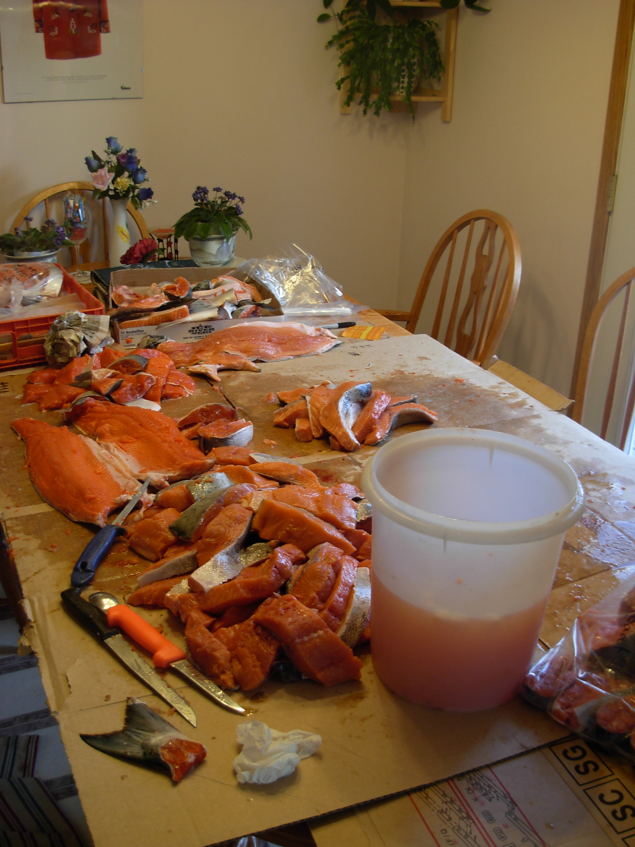
\includegraphics[width=0.7\textwidth]{figures/schreyer-fig2}
    \caption{Food Fish (July 2007) is being prepared for the T’aaku K̲wáan Dancers fund raising barbecue at the Atlin Arts and Music Festival}
    \label{schreyer-fig2}
\end{figure}


The Taku River Tlingit participated with their own dance group for the first time in 2006. I volunteered at the dance group’s barbecue at the Atlin Arts and Music Festival in 2006, 2007, and 2009, and they have consistently been very successful. I have also been privileged to join the T'aak̲ú K̲wáan Dancers in Juneau, Alaska for Celebration in 2006, 2008 and most recently, in 2014. During their stay in Juneau, the dance group has also begun to host a salmon barbecue on Sandy Beach on Douglas Island. Historically, this was an important locale for this K̲wáan (Thornton 2012) and they are renewing this coastal connection. Community members have also been renewing their inland Tlingit connection through the hosting of a salmon feast in Teslin, Yukon for the Inland Tlingit Celebration, which has run since 2011 in the odd-numbered years between Sealaska’s Celebrations. At the Inland Celebration, known as Hà Kus Teyea, each of the Inland Tlingit communities (Teslin Tlingit Council, Taku River Tlingit, and Carcross-Tagish First Nation) take turns hosting a feast. The Taku River Tlingit feast features salmon and they also host a salmon filleting contest earlier on the day of the feast, where contestants compete for the fastest filleting and best filleting skill awards.

As can be seen above, salmon helps to promote physical and mental health, as well as social connection. Similarly, in 2007, Wayne Carlick, dance leader and renowned carver, also developed a skit for the children’s dancers, Dikée Aankáawu Yátx’i (Children of the Creator), at the Atlin Arts and Music Festival that illustrated the ceremony associated with the first salmon caught each year down river. In this ceremony, to respect the salmon after it is eaten, the bones are placed back in the water to replenish the salmon for future generations. As Lakoff and Johnson write, “the metaphors we live by, whether cultural or personal, are partially preserved in ritual” (Lakoff and Johnson 1980: 234). Salmon, the bloodline of the Taku people, is therefore also helping to feed the spiritual and cultural well-being of the Taku River Tlingit people, as well as their physical well-being.

The connection between the Taku River and community health can also be seen in the community’s desire to keep the land healthy. In the Lands and Resources Department’s

Vision and Management document, Hà t\_tátgi hà khustìyxh - Our Land is Our Future, it is written, “Just as without land we cannot exist, without healthy land we can not be healthy people” (2003: 17). It is the land, particularly the Taku River, which makes people feel good and stay healthy. Terry Jack, who I mentioned earlier, told me that during the winter he misses the Taku and being on the land, and how he feels restless until he’s there again. Other people have mentioned this to me as well. Andy Williams, a former Spokesperson and Wolf Clan director and one of Mrs. Nyman’s sons, is another person who has told me about the connection he feels to the Taku River. Andy, who lives in Whitehorse, has said that he tries to get to the Taku as often as possible in the summer because it feels like home and his roots are there (Schreyer field notes 2006). During an interview with Sandra Jack, the Spokesperson or leader of the Taku River Tlingit First Nation in 2006, I asked if she ever has the time to make it to the Taku. Sandra replied:

\begin{quote}
I haven’t [been lately], no, but I’ve been down to the Taku. I did a fishing season when I was down there. It was really good because I ended up commercial fishing, and it was just a beautiful time. A lot of people talk about how it changes your life...or it really helps you to heal up more so you can get through the rest of the year, and do reasonably well, and take care of the other part of your life. For myself, I ended up going down there knowing that it was a special place, but not knowing really what to expect. I’d never commercial fished, you know, I’d never been out on the river.... I think what was really important though, what I walked away with was just that experience of being down the Taku, and there were a lot of people that were down there at the time, I think there might have been twenty Tlingits that were all commercial fishing. So, it was something new that we were all trying, not that we knew exactly what we were doing, we just knew that we’d done it before. I mean it’s got to be in our blood (laughing). So, we ended up getting down there and just getting out and enjoying the land, and enjoying the work. [Jack interview September 2006]
\end{quote}

From the above examples, it should be evident that the metaphor of the Heart of the Taku has been expanded amongst community members from knowledge of the landscape to the actions of individuals and I now discuss the implications for the community as a whole.

\section{Metaphors as Social Action}

Basso in his work on the hunting metaphors of the Western Apache people has written that, “one of the properties of any successful metaphor is that is can be refined and enlarged in different ways” (Basso 1996: 60). Potter has commented similarly that, “conceptual metaphors are generally imbricated---that is, overlapping and reinforcing---and operate at a variety of scales” (Potter 2003: 325). This can be seen in the expanded and extended metaphors of the Heart of the Taku that are used amongst the members of the Taku River Tlingit First Nation. While some might argue a connection to metaphor might be lost as the name is translated from the Tlingit T'aak̲ú Téix̲'i to the English meanings of the words, I disagree. English has become the language of the community and is the language that is most often used to promote stewardship throughout their territory. Darnell observed the role of English as a language for social action, when she argued that:

\begin{quote}
In the absence of political, economic, and personal empowerment, language comes to the forefront of the new traditionalism as a powerful symbol of Native-ness, of the right to reclaim lost skills and ways of life…But language enters the equation in another way which is at least as interesting. That is, language is also discourse, a discourse of social action and political empowerment. It is a discourse in English. [Darnell: 1994: 75]
\end{quote}

As noted above, the Taku River Tlingit First Nation has been a role model for other Indigenous communities in terms of their many court cases, documents, and government-to-government negotiations that promote themselves as the rightful stewards of their lands. Paul Nadasdy writes about the members of the Kluane Lake First Nation to the north in the Yukon:

\begin{quote}
If, in the context of the modern nation-state, aboriginal people wish to claim some form of control over their lands, and they wish those claims to be seen as legitimate by others, they must as Richard Handler puts it, speak “in a language that power understands” (1991: 71). And that language is, and has long been, the language of property. [Nadasdy 2002: 253]
\end{quote}

The language of property in this area of Canada is English and the Taku River Tlingit First Nation therefore use English geographic names to convey their own cultural concepts of property and heritage. In this way, the members of the Taku River Tlingit First Nation are using English, as well as Tlingit, to their advantage through the use of these metaphors and through performatives of stewardship. My definition of “performatives of stewardship” is \textit{actions that assert leadership and responsibility in caring for a community’s lands and resources and (re)define who has this responsibility in a particular territory. }This definition is based on Sullivan’s (2006) ideas “performatives of sovereignty” and is highly linked to the Taku River Tlingit First Nation’s own definitions of stewardship, which are outlined in their Vision and Management documents (TRTFN 2003). \

Austin examined the performative nature of language in his book How to Do Things with Words (1962). He described the way that “the issuing of an utterance is the performing of an action” (Austin 1962: 6). Austin separated utterances into illocutionary force (what the utterance does) and perlocutionary force (how the audience reacts). However, Mac Cormac writes that metaphors “often seem to fuse these into a single feature of language” (Mac Cormac 1985: 160). Mac Cormac sees metaphors then as a type of speech act, where one metaphorizes. He writes that:

\begin{quote}
Metaphors not only convey and stimulate meanings, but also perform significant actions. Metaphors suggest, convey, and generate emotions; puzzle; and often form an intimate bond between speaker and hearer (Mac Cormac 1985: 179).
\end{quote}

When this meaning moves beyond the individual to the larger community Mac Cormac says, “we can discover an additional dimension of meaning – that of cultural meaning” (Mac Cormac 1985: 178). This cultural meaning can be seen in the ways that the Taku River Tlingit community members have taken on the historical metaphor of the Heart of the Taku and applied it to contemporary physical, social, cultural, and economic domains. As I have written elsewhere, the genres of place that Taku River Tlingit community members use to promote stewardship in their territory can be seen as performatives of stewardship (Schreyer 2016). The polysemic, imbricated metaphors that are tied together via two languages are another performative of stewardship that community members are involved in, but these are tied to a very specific locale---the island, T'aak̲ú Téix̲'i or the Heart of the Taku.

\section{Conclusions}

Thornton, in the abstract for his chapter entitled, “Language and landscape among the Tlingit”, writes, “although the language is considered endangered, Tlingit toponyms and geographical nomenclature are well documented and many groups continue to occupy and use their traditional territory in ways that support traditional concepts of the lands and waters of their living space” (2011: 275). This is what I have been attempting to show for the specific place, T'aak̲ú Téix̲'i, the Heart of the Taku, located in Taku River Tlingit territory. However, the impact of language endangerment has made this discourse one that is also tied to English. In this chapter, Thornton also argues for a new understanding of the concept of “ecotope” or “the smallest ecologically-distinct landscape features” (Hunn \& Meilleuur 2010: 15ff), in order that, “cultural landscapes may come to be understood not simply as named sites but as a composition of meaningful places within a sociological system” (276). Thornton discusses islands as one particularly relevant type of ecotope within Tlingit society (2011: 284). Therefore, throughout this in-depth discussion of the numerous ways that the Heart of the Taku is understood and used by Taku River Tlingit community members, I feel that we can use this specific island as a case study of Thornton’s concept. Thornton includes four processes that affect how ecoptopes are viewed and understood. These are: perception, affordance, practice, and biospiritual forces (2011). I, therefore, review each of these processes in reference to the discussion provided above about the Heart of the Taku in order to discuss the specific ecotope of the Heart of the Taku.

First, Thornton discusses perception or the different ways that aspects of the landscape are categorized. Using the concept of embodiment from phenomenology, Thornton writes that:

Given this logic and the primacy of the body as instrument of landscape perception, we would expect to find widespread metaphorization and anatomical referencing of the body in the landscape. Indeed this is the case in Tlingit… (Thornton 2011: 278).

Thornton goes on to discuss the types of body parts that are referenced in Tlingit, which generally are those focusing on the head, and are often orifices. In his other work, Thornton has commented in regards to anatomical metaphors that Tlingit speakers seem to have a “marked preference for naming places after external bodily features, as opposed to internal ones” (2008: 97). He does note, however, the heart is one of the few internal organs he has seen represented (2008: 215). In terms of perception, the Heart of the Taku, is classified in relation to body parts, like many other Tlingit names, although it seems that its reference to an internal organ is rather special. Similarly, we should remember that the internal organ in question belongs to a giant, who is a powerful being from a different time period, rather than a human or an animal, and this may invoke different forms of perception.

Next, Thornton discusses the concept of affordance, which he describes as “a means of understanding how particular objects or environments ‘invite’ certain action possibilities and constrain others” (2011: 279). In particular, Thornton references Cruikshank’s work (2005), which examines the dialogues that occur between people and glaciers amongst Tlingit and Athapaskan groups (2011: 280). Similarly, a recent Taku River Tlingit community newsletter remarked, “Elders say, the land is alive. We just have to have the conversation. How? Be on the land. Be alive in it. Listen, and Talk” (TRTFN 2009: 1). As well, one of the motivations for the Learning to Talk to the Land participatory mapping project was so that community members could learn how to further develop their stewardship practices through learning how to call the land by its correct name (Schreyer et al 2014). When asked if she thought it was important for people to learn the correct Tlingit place names, Susan Carlick replied, \ “I think that our land would appreciate it” (Carlick, S., interview, 2011), which again shows that the land is inviting certain actions. T'aak̲ú Téix̲'i was one of the first places to be included within the Taku River Tlingit place names mapping project. There are more pictures included on the website for the Taku River, T'aak̲ú Héen, and T'aak̲ú Téix̲'i than any other place and during the design of the website it was important to our community research partners that photographs of T'aak̲ú Téix̲'i appear in the set of photos that circulate through the website’s cover page. This priority inclusion of T'aak̲ú Téix̲'i continues to illustrate the importance of this particular place name, locale, and ecotope.

The third process that Thornton discusses is practice, which he describes as the way in which people put the possibilities of dialogue from affordance into practice. He also states that, “an ecotope’s utility is a reflection of its practical significance to those who make a living from it” (2011: 281). In this case, the possibility that is enacted through the use of the place name of the Heart of the Taku and all of the associated metaphors is the practice of stewardship and respecting the land and the relationship people have to the land, which includes the plants and the animals that make their homes there. Thornton also states that, “another critical dimension of ecotope conceptualization was cultural keystone species (Garibaldi \& Turner 2004)” (2011: 282). As mentioned above, one of the metaphors that is associated with the Heart of the Taku is the set of extended metaphors of bloodline, lifeblood and lifeline and one of the meanings associated with these is a keystone species from the Taku River, salmon.

Last, Thornton discusses the concept of biospiritual forces, or the animate and powerful spirits that are a part of the landscape. He writes that similar to other animistic societies, “So it is in Tlingit country, where the oceans, rivers, mountains, glaciers, and a variety of other landforms were considered alive or animated by spirits to whom one could appeal (Swanton 1908; de Laguna 1972)” (Thornton 2011: 283). As mentioned previously, the origins of the name the Heart of the Taku come from the mythohistoric time of the giants, but beyond this there is the conception that the land is listening. As well, the respect for the land and the biospiritual forces can be seen in the ceremony, which is performed at the Taku River, where the first salmon bones of the fishing season are put back into the river to help sustain its power and life force.

In sum, T'aak̲ú Téix̲'i, the Heart of the Taku, fits well within Thornton’s concept of an ecoptope. The metaphors that the community members are using are further embedding their concepts of stewardship within both the Tlingit language and the language of English through the processes of perception, affordance, practice, and biospiritual forces. In his discussion of performatives, Austin (1962) also discussed what he called “the felicity condition”, which means that in order for the performative to be completed it has to be both heard and understood to be a performative by the listener. As the language of stewardship in this community has often been tied to English, performatives through English metaphors are a necessary part of this felicity condition. As a result, the multi-layered meanings of T'aak̲ú Téix̲'i, and specifically, the English Heart of the Taku, means that insiders and outsiders to the community may have a different understanding of this ecotope depending not only on where they stand, but where their ancestors have stood and how they have engaged this landscape since time immemorial.




\section*{Acknowledgments}

I would like to say gunalchéesh, thank you, to the members of the Taku River Tlingit First Nation for being my research partners and friends. I am honored to work with you and learn from you. I would also like to thank Gary Holton and Thomas Thornton for asking me to participate in this volume honoring James Kari. I am grateful to the two reviewers who provided feedback on my paper; any remaining errors are mine alone. Financial support for this research was provided by: SSHRC, the Northern Scientific Training Program, the Canadian Circumpolar Institute, and the University of British Columbia.


\refheading
\begin{hang}


Austin, J.L. 1962. \textit{How To Do Things With Words}. Oxford: Clarendon Press.

Basso, Keith. 1996. \textit{Wisdom Sits in Places: Landscape and Language Among the Western Apache.} Albuquerque: University of New Mexico Press.

BC Parks. 2012. Taku River/T’akú Téix’ Conservancy  \url{http://www.env.gov.bc.ca/bcparks/explore/cnsrvncy/taku-rv/}, accessed September 5, 2014.

Canadian Press. 2015. BC Upholds Environmental Certificates for Controversial Mines. January 14, 2015  \url{http://www.ctvnews.ca/business/b-c-upholds-environmental-certificates-for-controversial-mines-1.2189673}

Crippen, Julie. 2010. The New Tlingit Dictionary: An Encyclopedia Dictionary of the Tlingit Language. Unpublished document: \url{http://www.drangle.com/~james/dictionary/}

Cruikshank, Julie.  2005. \textit{Do Glaciers Listen? Local Knowledge, Colonial Encounters and Social Imagination}. Vancouver: UBC Press.

Darnell, Regna. 1994. Private Discourse, Public Discourse, and Algonquian Oral Tradition. In Papers of the Algonquian Conference -Volume 25. W. Cowan, ed. Pp. 72-82. Ottawa: National Museum of Canada.

de Laguna, Frederica. 1972. \textit{Under Mount St. Elias: The History and Culture of the Yakutat Tlingit}. 3 vols.  Washington DC: Smithsonian Institute Press.

EcoJustice. 2014. BC Government Violated duty to consult Taku River Tlingit Regarding Controversial  Tulsequah Chief Project. \url{http://www.ecojustice.ca/media-centre/press-releases/bc- government-violated-duty-to-consult-taku-river-tlingit-regarding-controversial-ulsequah-chief-project}

Garibaldi, Ann \& Nancy Turner. 2004. Cultural Keystone Species: Implications for Ecological Conservation and Restoration.  \textit{Ecology and Society} 9(3). 1-18.

Goldschmidt, Walter, Theodore, Haas \& Thomas Thornton. 1998.  \textit{Haa Aaní – Our Land: Tlingit and Haida Land Rights and Use}. Seattle: University of Washington Press.

Handler, Richard. 1991. Who owns the Past? History, Cultural Property, and the Logic of Possessive  Individualism. In Brian Wallace (ed.), \textit{The Politics of Culture},  63-74. Washington DC: Smithsonian Institute Press.

Hunn, Eugene S. \& B. Meilleur. 2010. Toward a Theory of Landscape Ethnoecological Classification. In Leslie M. Johnson \& Eugene S. Hunn (eds.), \textit{Landscape Ethnoecology},  15-26. New York: Berghan.

Indian Country Today Media Network. 2011. Taku River Tlingit First Nation Balances Stewardship with Development in Historic Deal with B.C. \url{http://indiancountrytodaymedianetwork.com/2011/08/13/taku-river-tlingit-first-nation-balances-stewardship-development-historic-deal-bc-46972}, accessed January 17, 2014

Kari, James. 1996a. A Preliminary View of Hydronymic Districts in Northern Athabaskan Prehistory. \textit{Names} 44(4). 253-271.

Kari, James. 1996b.  Names as Signs: ‘Mountain’ and ‘Stream’ in Alaskan Athabaskan Languages. In E.  Jelinek, S. Midgette, K. Rice \& L. Saxon (eds.), \textit{Athabaskan Language Studies, Essays in Honor of Robert W. Young}, 443-75. Albuquerque:  University of New Mexico Press.

Lakoff, G \& Mark Johnson. 1980. \textit{Metaphors We Live By}. Chicago: University of Chicago Press.

Mac Cormac, Earl R. 1985. \textit{A Cognitive Theory of Metaphor}. Cambridge: The MIT Press.

Nadasdy, Paul. 2002. “Property” and Aboriginal Land Claims in the Canadian Sub Arctic: Some  Theoretical Considerations. \textit{American Anthropologist} 104(1). 247-261.

Nyman, Elizabeth \& Jeff, Leer. 1993. \textit{Gagiwdul.at: Brought Forth to Reconfirm: The Legacy of a Taku River Tlingit Clan}.
 Whitehorse \& Fairbanks: Yukon Native Language Centre \& Alaska Native Language Center.

Potter, James M. 2003. Creation of Person, the Creation of Place: Hunting Landscapes in the American Southwest. \textit{American Antiquity} 69(2). 322-338.

Rivers Without Borders. 2014. Lawsuit from Taku River Tlingit First Nation Threatens Proposed Tulsequah Chief  Mine. \url{http://riverswithoutborders.org/blog/2014/02/lawsuit-from-taku-river-tlingit-first-nation-threatens-proposed-tulsequah-chief-mine}, accessed September 5\textsuperscript{th}, 2014

Schreyer, Christine. 2016. Taku River Tlingit Genres of Places as Performatives of Stewardship. \textit{Journal of Linguistic Anthropology} 26(1). 4--25.

Schreyer, Christine. 2014. Canadian Geography as National Identity: Hudson’s Bay Company Place Names and  their Aboriginal Counterparts. \textit{International Journal of Canadian Studies} 49(1). 315--34.

Schreyer, Christine, Jon, Corbett, Nicole, Gordon \& Colleen Larson. 2014. Learning to Talk to the Land: Online Stewardship in Taku River Tlingit Territory. \textit{Decolonization: Indigeneity, Education, and Society } 3(3). 106--133.

Swanton, John R. 1908. Social condition, beliefs, and linguistic relationships of Tlingit Indians. In \textit{Twenty-sixth Annual Report, Bureau of American Ethnology}, 391-485. Washington DC:  Government Printing Office.

Sullivan, Kathleen M. 2006. (Re)Landscaping Sovereignty in British Columbia, Canada. \textit{PoLAR: Political and Legal Anthropology Review}  29(1). 44-65.

Supreme Court of Canada. 2004. Taku River Tlingit First Nation v. British Columbia (Project Assessment Director), [2004] 3 S.C.R. 550, 2004 SCC 74

Taku River Tlingit First Nation and BC Wild. 1997. Taku: Will a short-lived mining project sever the \textit{bloodline }of the Tlingit people? Booklet.

Taku River Tlingit First Nation. 2014. Aboriginal Languages Initiative Assessment. \url{http://maps.fphlcc.ca/node/3152}

Taku River Tlingit First Nation. 2011. Wóoshtin wudidaa - Atlin Taku Land Use Plan. Atlin, British Columbia.

Taku River Tlingit First Nation. 2009. Tlatsini Map. Atlin, British Columbia.

Taku River Tlingit First Nation. 2007. Mining Policy. Atlin, British Columbia.

Taku River Tlingit First Nation. 2003. \textit{Our Land is Our Future - Hà t\_tátgi hà khustìyxh. Vision and Management Document for the Taku River Tlingit First Nation Lands and Resources Department.} Atlin, British Columbia.

Taku River Tlingit First Nation. 1997. Taku. Film.

Taku River Tlingit First Nation. 1993. Constitution. Atlin, British Columbia.

Taku Wild. 2014. \url{http://www.takuwild.com/}

Thornton, Thomas F. 2008. \textit{Being and Place Among the Tlingit}. Seattle, WA: University of Washington Press.

Thornton, Thomas F.. 2011. Language and Landscape among the Tlingit. In David. M. Mark, Andrew, G Turk, Niclas Burenhult \& David Stea (eds.), \textit{Landscape in Language: Transdisciplinary Perspectives},  289-304. Amsterdam/Philadelphia: John Benjamins.


Thornton, Thomas F.  2012. \textit{Haa Leelk’w Has Aaní Saax’u: Our Grandparents’ Names on the Land}. Juneau \&  Seattle: Sealaska Heritage Institute and University of Washington Press.

Williams, Jackie. 2013. \textit{Lingít Kusteeyí: What My grandfather taught me}. Atlin, BC: Taku River Tlingit First  Nation.


\end{hang}

\begin{center}
\textbf{List of Interviews}
\end{center}

\begin{hang}
Carlick, Alice. 2006. Interview with Christine Schreyer. Atlin, British Columbia, June, 2006.

Carlick, Susan. 2011. Interview with Christine Schreyer. Atlin, British Columbia, June 2011

Gordon, Louise. 2006. Interview with Christine Schreyer. Atlin, British Columbia. June, 2006.

Jack, Sandra. 2006. Interview with Christine Schreyer. Atlin, BC, September 2006

\end{hang}

\bigskip

\orcidfooter{Christine Schreyer}{christine.schreyer@ubc.ca}{}

\label{schreyer-ch-end}


     \chapter[Directional Reference in Discourse and Narrative]{\vspace{-25pt}Directional Reference in Discourse and Narrative: Comparing indigenous and non-indigenous genres in Ahtna}

\sethandle{10125/24842}

% \usepackage[
% 	doi=false,
% 	backend=biber,
% 	natbib=true,
% 	style=biblatex-sp-unified,
% 	citestyle=sp-authoryear-comp]{biblatex}
%\usepackage[style=ldc.bst]{biblatex}



% Author last name as it appears in the header
\def\authorlast{Berez-Kroeker}

% change author in three references below to the actual author name so that this name is unique and matches the \label commands just below and at the end of the chapter
\renewcommand{\beginchapter}{\pageref{berez-ch-begin}}
\renewcommand{\finishchapter}{\pageref{berez-ch-end}}
\label{berez-ch-begin}



\thispagestyle{firststyle}

\chapauth{Andrea L. Berez-Kroeker}
\affiliation{University of Hawai‘i at Mānoa}

\authortoc{Andrea L. Berez-Kroeker}



\section{Introduction}\hspace{-0.3cm}\footnote{Many thanks to Jim Kari, Marianne Mithun and Sandy Thompson for their comments on this paper, parts of which also benefited greatly from discussion at seminars in the linguistics departments at the University of Melbourne and the University of Sydney. Errors herein are the fault of the author alone. Funding was provided by the University of California Pacific Rim Research Program, the American Philosophical Society, and the Jacobs Research Fund. This paper is meant to honor not only Jim, but also the memory of Markle Pete, whose warm heart and hearth will not be forgotten.}

This paper examines the role of culture in the grammar of motion events in Ahtna, with particular attention to the efficacy of “frog story” experiments in eliciting that grammar. Since the mid-1990s, linguistics has seen a proliferation of literature based on frog story experiments. In this research paradigm, speakers of various languages are shown a textless children’s book of drawings called \textit{Frog, Where are You?} \citep{Meyer1969} and are asked to narrate the events depicted there in their native tongue.\footnote{Frog story research developed out of the desire to make typological comparisons across languages. Because direct translations from a contact language can often distort the native grammar, one solution has been to present speakers of different languages with the same nonlinguistic stimulus in order to elicit spontaneous speech, which is more likely to reveal authentic grammatical constructions.} The story is about a boy and his dog who search through the woods for a pet frog that had escaped from its glass jar during the night. The boy and the dog undergo a series of adventures in which they encounter a host of forest dwelling creatures, including a squirrel, a swarm of angry bees, an owl, and a buck. The characters move from place to place, starting with a fall from the bedroom window and ending climactically with a ride atop the buck’s horns and a tumble from a cliff into a river.

Over the years, narratives resulting from frog story experiments have been used as the basis for inquiry into a wide range of topics in linguistics and psychology. Among these, the study of the expression of direction or path description in language – has garnered much attention. The research, summarized in \citet{Slobin2004}, stems from the work of  \citet{Talmy1985,Talmy1991,Talmy2000}, who presents a typology of the lexicalization of semantic units and the patterns of conflation of those units (i.e., \textsc{motion} \textsc{+} \textsc{manner,} \textsc{motion} \textsc{+} \textsc{path,} \textsc{motion} \textsc{+} \textsc{figure}). \citet{SV2004} is a collection of studies aiming to apply this typology to Warlpiri, Basque, Tzeltal, Icelandic, West Greenlandic, Swedish, Thai, American Sign Language, and Arrernte.

Among these, \citet{Wilkins2004} in particular finds that extralinguistic ethnographic considerations are very closely tied to grammar in his study of frog stories in Arrernte, a language of Central Australia. He shows that even within the genre of frog stories, Arrernte culture is a better predictor than language type of motion event segmentation. According to Slobin’s typology, one could hypothesize that Arrernte speakers devote less attention to the dynamic description of direction than would speakers of other types of languages \citep[see][]{Slobin2004}. Conversely, though, based on the nomadic culture of Desert Aborigines and the prominence of travel in everyday life, one could also hypothesize that Arrernte speakers will pay special attention to routes of motion and should construct elaborately detailed direction descriptions (see \citealt{Wilkins2004} for the argumentation). Wilkins shows that the latter is true: Arrernte speakers segment the direction description into more distinct trajectories in frog stories than English speakers. The difference is both quantitative in terms of path complexity and qualitative in terms of the kinds of linguistic structures used by speakers. As Wilkins writes, “[t]hus, it is the areal ethnographic observations … which here appear to be more predictive of the findings [i.e., than the typological predictions]” (2004: 155). The role of culture on the development of grammar should not be underestimated.

This paper examines the role that cultural considerations play in the grammar of motion events in Ahtna, and finds that frog stories are not the most effective tool for eliciting that grammar. The Ahtna community today consists of eight modern villages (Mentasta, Chistochina, Gakona, Gulkana, Tazlina, Copper Center, Chitina, and Cantwell) in the Copper River and Upper Susitna drainages of south central Alaska. In the 1980s and 1990 Jim Kari was responsible for the lion’s share of documentation and description of the language, and still continues to publish and work with speakers today.

Ahtna society is traditionally semi-nomadic. Hunters and family groups traveled seasonally in pursuit of resources like fish and big game (\citealt{Reckord1979}, \citeyear{Reckord1983a}, \citeyear{Reckord1983b}). Knowledge of the surrounding terrain is not only essential to survival but also plays an important role in ethnic identity and the assertion of the connection of one’s social group (tribe, band, family) to the land, much like \citet{MooreTlen2007} found for Athabascan speakers in the Yukon. Individual Ahtna men – and some women – are often intimately familiar with large swaths of the 35,000 square miles of Ahtna territory and beyond, a feat all the more impressive for having been undertaken on foot or by dogsled.

The importance of geographic knowledge and ‘travel talk’ is reflected in the sheer size of the corpus of Ahtna place names (\citealt{Kari1982}, \citeyear{Kari2008}). The corpus contains over 2,200 names, many of which are documented in a genre of oral literature that Kari terms \textit{elite travel narratives}. These narratives are a kind of “virtual guided tour” in which the speaker discusses, in sequential order, all the meaningful and hence named locations along a given route. A single narrative may cover over one hundred miles of river and/or trail and is often interspersed with personal memories and descriptions of how each site was used seasonally for camping and hunting (for published examples of Ahtna travel narratives see \citealt{Kari1986}; \citealt{KariFall2003}; \citealt{Kari2010}).

In some superficial ways, frog stories and Ahtna travel narratives are similar: animate referents move across the countryside in pursuit of animal(s). But in many ways, particularly cultural ways, they are different. In \textit{Frog, Where Are You?}, referents engage in activities that do not happen everyday: heads get stuck in jars, characters fall out of windows and trees and off cliffs, owls and gophers pop suddenly out of their holes, and characters interact with rather unfriendly bucks and bees. In travel narratives, on the other hand, activities are generally limited to walking, sledding, hunting, and camping.

As is discussed below, speakers telling travel narratives make full use of the grammar of path and location available to them, including adverbial verb prefixes, a class of riverine directionals, and highly systematic toponymy. Interestingly, while all of these (with the exception of possibly toponymy) are also available to frog story narrators, speakers in this genre seem to restrict themselves to only a narrow range.

What role, then, does genre (e.g. \citealt{Mayes2003}) play in an academic study of how a language encodes notions of direction and location in motion events? Can a frog story fully reveal the nature of Ahtna grammar about motion? Or will other concerns, specific to the tasks of telling a frog story or a travel narrative, be more important and ultimately influence where a speaker’s attention lies? The following sections examine two Ahtna travel narratives and an Ahtna frog story with an eye toward answering these questions.

The first travel narrative was recorded in 1980 by Jake Tansy with linguist James Kari. Mr. Tansy describes an overland and riverine hunting route, used exclusively in the summertime, from the mouth of Alaska’s Brushkana River to the Yanert Fork and onward to Valdez Creek. In Ahtna the story is called \textit{Saen} \textit{tah} \textit{xay} \textit{tah} \textit{c’a} \textit{łu’sghideł} ‘we used to travel around in summer and winter’ \citep[59-69]{Kari2010}; henceforth Mr. Tansy’s monologue is referred to as \textit{Saen} \textit{tah} \textit{xay} \textit{tah}  (‘during summer and winter’).

The second narrative was recorded by Adam Sanford in 1986, also with Kari. This is an epic description of yearly hunting routes, often in the extreme mountainous highlands in pursuit of Dall sheep. The entire recording is nearly thirty minutes in length; only the first five minutes are presented here. This narrative is known in Ahtna as \textit{C’uka} \textit{ts’ulaen’i} \textit{gha} \textit{nen’} \textit{ta’stedeł} \textit{dze’} ‘how we went hunting out in the country’ \citep[91-128]{Kari2010}. Henceforth this narrative is referred to as \textit{Ta’stedeł} \textit{dze’} (‘we went hunting thus’). Finally, the narration of \textit{Frog,} \textit{Where} \textit{Are} \textit{You?}---in Ahtna \textit{Naghaay,} \textit{ndaane} \textit{zidaa}, and henceforth \textit{Naghaay} (‘frog’)---was recorded in October 2008 in Tazlina, Alaska by Ahtna speaker Markle Pete with the author.

Section 2 below compares the distribution of the spatially oriented grammatical systems across the two genres. I first look at the use of direction- and location-describing adverbial verb prefixes, a mechanism that is employed by all three speakers. I then look at two areas of the grammar where the stories differ, the use of directionals and toponymy. While all three systems are fully utilized by travel narrators, Mr. Pete makes very limited use of the last two in \textit{Naghaay}.

The unequal use of spatial grammar in the two genres reflects the speakers’ unequal attention to figure and ground. Section 3 examines how the storytelling tasks that the speakers deem important influence the choices they make when structuring discourse. Mr. Tansy and Mr. Sanford foreground the spatial and temporal trajectories of their narratives, while Mr. Pete elects instead to carefully track referents, which is common in frog-story narration worldwide.

Section 4 contains concluding remarks about the role of genre in typology and language documentation. Ultimately it seems Mr. Pete’s concerns may not lie in creating a fully elaborated sense of the fictional landscape in \textit{Frog,} \textit{Where} \textit{Are} \textit{You?}, which in turn affects how well the story reveals Ahtna’s path-describing grammatical systems. As is discussed below, works of oral literature in Ahtna are often a-spatial.

\section{Grammar of Direction and Location in \textit{Saen} \textit{Tah} \textit{Xay} \textit{Tah,} \textit{Ta’stedeł} \textit{Dze’,} and \textit{Naghaay}}

This section describes three mechanisms for elaborating direction and location in Ahtna: adverbial verb prefixes, riverine directionals, and toponymy. It compares the travel narratives to the frog story in terms of each of these linguistic resources.

\subsection{Derivational/Thematic Adverbial Prefixes}

Ahtna, like all Athabascan languages, is a polysynthetic language with templatic verbal morphology. Table~\ref{berez:tab:1} shows a simplified version of the verb template from \citet{Kari1990}. Verbs are stem-final, with eleven prefix zones (further analyzable into up to twenty-eight individual slots) to the left of the stem. Near the far left edge, in position ten, we find the so-called ‘derivational/thematic’ prefixes. Many of the morphemes here are adverbial in function and can describe, among other things, path and location. Kari writes of the morphemes found here, “nearly one hundred morphemes appear in this position \ldots includ[ing] bound postpositions” (1990:40), which provides insight into the source of the spatial nature of these prefixes. The morphemes in this position that were historically free preverbal postpositions are grammaticalizing; they are undergoing phonological fusion to the verb, losing their objects, and becoming less adpositional and more adverbial in function.

\begin{table}[ht]\centering
\caption{Ahtna Verb Template (adapted from \citealt{Kari1990})}
\label{berez:tab:1}
\begin{tabular}{| *{12}{ l | }}
\hline
\rotatebox{90}{Bound postpositional object\ \ } &
\rotatebox{90}{Derivational/Thematic} &
\rotatebox{90}{Iterative} & \rotatebox{90}{Distributive} & \rotatebox{90}{Incorporate} & \rotatebox{90}{Thematic} & \rotatebox{90}{Pronominal} & \rotatebox{90}{Qualifiers} & \rotatebox{90}{Conjugation} & \rotatebox{90}{Subject} & \rotatebox{90}{Classifier} & \rotatebox{90}{Stem}\\

\hline
11 & 10 & 9 & 8 & 7 & 6 & 5 & 4 & 3 & 2 & 1 & \\
\hline
\end{tabular}
\end{table}


In \textit{Saen} \textit{tah} \textit{xay} \textit{tah}, \textit{Ta’stedeł} \textit{dze’}, and \textit{Naghaay}, all three speakers make extensive use of direction-describing adverbial prefixes. Of the seventy-eight motion verbs in the three stories, only four have no such prefix. Furthermore, the prefixes occur with uniform density. In \textit{Saen} \textit{tah} \textit{xay} \textit{tah} twenty-one of twenty-four motion verbs contain at least one direction- or location-describing prefix; the ratio in \textit{Ta’stedeł} \textit{dze’} is twenty-one of twenty-two motion verbs; and in \textit{Naghaay}, thirty-two of thirty-two motion verbs. These distributions do not differ significantly.

In contrast to the highly precise directional system, the adverbial prefixes usually describe simple paths of motion of the subject. In the examples from \textit{Saen} \textit{tah} \textit{xay} \textit{tah} and \textit{Ta’stedeł} \textit{dze’} shown in (1-2), the prefixes encode the simple directions of ‘away’, ‘out’, ‘through’, ‘back’, and ‘up’.

%ex1
\begin{exe}
  \ex   Direction-describing adverbial verb prefixes in \textit{Saen tah xay tah}\footnote{Transcription conventions and abbreviations are found in the Appendix.}\label{berez-ex1}
\begin{xlistn}
\exi{01} \gll Xona,\\
    now\\
\sn \begin{flushright} (0.6) \end{flushright}
\exi{02}  first
\begin{flushright} (0.9) \end{flushright}
\exi{03} \gll   nen’ \textbf{ta}’stghideł de c’a saen ta, \\
    country   1\textsc{pl.sub}.pl.go.\textbf{away}  when  \textsc{foc}    summer  during\\
\sn \begin{flushright} (0.9) \end{flushright}

\exi{04} \gll c’a  Bes Ggeze Na’, \\
    \textsc{foc}  bank   worn     stream.\textsc{pos}\\
\sn \begin{flushright} (0.4) \end{flushright}
\exi{05} \gll  Saas Nelbaay Na’,\\
    sand  grey      stream.\textsc{pos}\\
\exi{06} \gll hwcets’edeł. \\
    1\textsc{pl.sub}.ascend\\

\glt \textit{‘When we first went out in the country during the summer we would go to the base of ‘Worn Bank Stream’ or ‘Sand That is Grey Stream’.’}
\sn \begin{flushright} (1.5) \end{flushright}
\exi{07} \gll       Niłdenta łu,\\
    sometimes  \textsc{evid}\\
\sn \begin{flushright} (0.6) \end{flushright}
\exi{08} \gll  Dghateni    yi ’eł tanidzeh,\\
    stumbling.trail  3s  \textsc{conj}   middle.water\\
\exi{09} \gll      Dghateni \textbf{ts’i}diniłen.\\
    stumbling.trail  water.flows.\textbf{out}\\
\glt \textit{‘Sometimes also to ‘Stumbling Trail’ or the middle one flowing out from ‘Stumbling Trail’.’}

\sn  \ldots

\exi{43} \gll  dets’en,\\
    next\\

\exi{44}    \gll    Nts’ezi Na’ ba’aa,\\
    N.       stream.\textsc{pos}  outside\\

\exi{45}    \gll    dghilaay   \textbf{gha}kudaan de \textbf{ka}nats’edeł n'eł,\\
        mountain   hole.extends.\textbf{through} where \textsc{1pl.sub}.pl.go.\textsc{iter}.\textbf{up}  \textsc{conj} \\

\glt \textit{‘outside of ‘Nts’ezi’s Stream’ we went back up where a tunnel extends through the mountain, (and \ldots)’}

\end{xlistn}

\begin{flushright}
((Jake Tansy, \textit{Saen} \textit{Tah} \textit{Xay} \textit{Tah} \textit{C’a} \textit{Łu’sghideł\\
‘We} \textit{Used} \textit{to} \textit{Travel} \textit{Around} \textit{in} \textit{Summer} \textit{and} \textit{Winter’},\\
00:00:05.580-00:01:20.650. \citealt{Kari2010}:60-61))
\end{flushright}

\end{exe}

%ex2
\begin{exe}
 \ex Direction-describing adverbial verb prefixes in \textit{Ta’stedeł dze’}\label{berez-ex2}
 \begin{xlistn}
\exi{127} \gll {K’a xona} 	yet		hwts’en	xona	\textbf{na}’stetnaesi,\\
		then			there	from.area	then		1\textsc{pl}.travel.nomadically.\textbf{back}\\
\sn \begin{flushright}(2.3)\end{flushright}
\exi{128} \gll			ohh	dahwtnełdak. \\
		oh		3\textsc{s}.be.steep\\
		\textit{‘Then as we moved back from there, oh it (the canyon) was steep.’}
\sn \begin{flushright}(0.6)\end{flushright}
\exi{129} \gll			Niłk’aedze’	dahwtnełdak	xona, \\
		both.sides		3\textsc{s}.be.steep		then\\
\sn \begin{flushright}(0.8)\end{flushright}
\exi{130}	\gll		saanetah	kats’enaes. \\
		barely		1\textsc{pl}.trave.nomadically.up\\
\glt	\textit{	‘It was steep on both sides and then we could barely move up.’}

\end{xlistn}
\begin{flushright}
((Adam Sanford, \textit{C’uka Ts’ul’aen’i gha Nen’ Ta’stedeł dze’}\\
\textit{‘How We Went Hunting Out in the Country’},\\
00:03:56.740-00:04:06.320. Kari 2010:96))
\end{flushright}
\end{exe}

\noindent
The semantic generality of the prefixes allows them to be used in a range of situations, not only describing a journey across the countryside as in (1-2), but also for the up-and-out motion of a squirrel from his den and the downward orientation of a bees’ nest hanging from a tree branch, as in the excerpt from \textit{Naghaay} in (\ref{berez-ex3}).


%ex3
\begin{exe}
\ex Direction-describing adverbial verb prefixes in \textit{Naghaay}\label{berez-ex3}
\begin{xlistn}
\exi{13} \gll	Łic’ae	gilok'ae	naghalts’et.\\
		dog		window		3S.falls.down\\
	\glt	\textit{‘The dog falls down from the window.’}
\sn {[ \ldots ]}
\exi{22}	\gll			Dligi	kaniyaa,\\
		squirrel	3S.go.up.and.out\\
\glt	\textit{	‘A squirrel comes up,’}
\exi{23} \gll			łic’ae	ngga	t’ox 	naggic’eł’i			gha		itsae.\\
		dog		upland	nest		3S.hang.down.REL	at		3S.bark\\
\glt		\textit{‘the dog barks at the nest that is hanging (there).’}
\end{xlistn}
\begin{flushright}
((Markle Pete, \textit{Naghaay Ndaane Zidaa} ‘Frog Where Are You’,\\
oai.paradisec.org.au:ALB01-AHTNB001-060.tiff,\\
ALB01-AHTNB001-061.tiff))
\end{flushright}
\end{exe}

\noindent
Based on the uniform density of spatially oriented prefixes in all three narratives, it would be reasonable to claim that frog story experiments do indeed exemplify how Ahtna speakers use prefixes to describe direction concepts in discourse. However, other data shows that \textit{Naghaay} does not provide us with a complete picture of how richly speakers can describe direction and location in Ahtna. The next section discusses the use of the directional system that is employed extensively in the travel narratives, and only minimally in \textit{Naghaay}.\footnote{It should be made clear that the reason Mr. Pete makes only limited use of the grammar of path and location because he is that he is expertly attending to other concerns, and not because he is in any way unfamiliar with his language.}

\subsection{Directionals}

Like other Athabascan languages, Ahtna has a set of directionals that can be defined as a separate lexical class based on their morphological behavior. Ahtna directionals have a tripartite structure shown in Table~\ref{berez:tab:2}: a stem expressing orientation (a system that is largely, but not completely, riverine; ‘up’ and ‘down’ are included in the paradigm on morphological grounds), an optional prefix expressing relative distance, and an optional suffix that expresses either a point-versus-area distinction or a path toward or away (see \citealt{Kari1985}, \citeyear{Kari1990}; \citealt{Leer1989}; \citealt{MooreTlen2007}).

\begin{table}
\centering
\caption{Tripartite structure of Ahtna directionals \citep[from][]{Kari1990}}
\label{berez:tab:2}
\begin{tabular}{ >{\raggedright\arraybackslash}p{4cm} | >{\raggedright\arraybackslash}p{4cm} | >{\raggedright\arraybackslash}p{4cm} }
\textbf{Prefixes} & \textbf{Stems} & \textbf{Suffixes}\\
\hline
\makecell[c{p{4cm}}]{
\textit{da-} ‘near’\\
\textit{na-} ‘intermediate distance’\\
\textit{’u-} ‘distant’\\
\textit{ts'i-} ‘straight, directly’\\
\textit{ka-} ‘next to’\\
\textit{P+gha-} ‘from P’\\
\textit{n-} ‘neutral’\\
\textit{hw-} ‘area’
}

&

\makecell[l]{
\textit{nae’} ‘upriver, behind’\\
\textit{daa’} ‘downriver’\\
\textit{ngge’} ‘from water, upland’\\
\textit{tsen} ‘toward water, lowland’\\
\textit{naan} ‘across’\\
\textit{tgge’} ‘up vertically’\\
\textit{igge’,} yax ‘down vertically’\\
\textit{’an} ‘away, off’\\
\textit{nse’} ‘ahead’
}
&
\makecell[l]{
\textit{-e} ‘to’\\
\textit{-dze} ‘from’\\
\textit{-t} ‘at a point’\\
\textit{-xu} ‘in a general area’\\ \\ \\ \\
}

\end{tabular}\end{table}


Examples of fully inflected directionals are found in (\ref{berez-ex4}).

\begin{exe}
\ex Examples of fully inflected directionals \label{berez-ex4}

\begin{xlist}


\ex \gll \textit{’u-ngge} \\
distant-upland  \\
\glt ‘distantly upland’


\ex \gll \textit{na-naa} \\
intermediate.distance-across  \\
\glt ‘an intermediate distance across’

\ex \gll \textit{’u-naa-ts’en}\\
distant-across-from \\
\glt ‘from distantly across’

\ex \gll \textit{’u-tsuu-ghe}\\
distant-lowland-general.area \\
\glt ‘in a general area distantly lowland’

\ex \gll ’u-ngga-t\\
distant-upland-at.point \\
\glt ‘at a point distantly upland’

\ex \gll \textit{ka-naa}\\
general.area-across \\
\glt ‘an area across’

\ex \gll \textit{’u-tsii-t}\\
distant-lowland-at.point \\
\glt ‘at a point distantly lowland/downland’

\end{xlist}

\end{exe}

\noindent
The morphological structure of the lexical class of directionals potentially allows speakers to be very precise in describing paths and locations in terms of their relationship to the placement and flow of the local river. In addition, the structure of Ahtna discourse allows even more specificity. Speakers very often use multiple directionals in a single clause to describe changes in trajectory or to pinpoint a destination precisely.\footnote{For more on the use of directionals in Ahtna discourse, see \citet{Berez2011,Berez2014}.} In (\ref{ex:key:5}), Mr. Tansy uses multiple directionals, in addition to adverbial prefixes, to describe a complex path with several trajectory changes (downriver – across – downriver – back).

%ex5
\begin{exe}
\ex Use of directionals in \textit{Saen tah xay tah} \label{ex:key:5}
\begin{xlistn}
\exi{25} \gll 		Niłdenta	łu’,\\
		sometimes	\textsc{evid}\\
\sn \begin{flushright}(0.7)\end{flushright}
\exi{26} \gll 				yet,\\
		there\\
\sn \begin{flushright}(0.8)\end{flushright}
\exi{27}	\gll 			Tl’ahwdicaax 			Na’, \\
		headwaters.be.valuable	stream.\textsc{pos}\\
\sn \begin{flushright}(0.4)\end{flushright}
\exi{28}	\gll 			’udaa’a,\\
		distant.downriver \\
\sn \begin{flushright}(0.5)\end{flushright}
\exi{29}	\gll 			’unaa			daa’a		ts’its’edeł	dze’	dae’, \\
		distant.across	downriver	1PL.go.out			thus\\
\exi{30}	\gll 			Nts’ezi		Na’			hwts’e’, \\
		N.			stream.\textsc{pos}	from.area\\
\sn \begin{flushright}(0.6)\end{flushright}
\exi{30}	\gll 			tes 		ninats’edeł.\\
		pass		1\textsc{pl}.go.back.to.a.point\\
\glt \textit{‘Sometimes then, we come out downstream and across and downstream of ‘Valuable Headwaters Stream’ and we come back to a pass at ‘Nts’ezi’s Stream’.’}
\end{xlistn}

\begin{flushright}
((Jake Tansy, \textit{Saen Tah Xay Tah C’a Łu’sghideł}\\
\textit{‘We Used to Travel Around in Summer and Winter’},\\
00:00:46.710-00:00:57.290. Kari 2010:61))
\end{flushright}
\end{exe}

\textit{Saen} \textit{tah} \textit{xay} \textit{tah} contains twenty-two directionals over 100 lines, and \textit{Ta’stedeł} \textit{dze’} contains twenty-six directionals over 218 lines. \textit{Naghaay}, however, contains only five (over 55 normative sentences). Of the handful of directionals found in \textit{Naghaay}, three occurrences are the use of \textit{ngge’} ‘upland’ to describe the location of the bees’ nest. The nest is not actually upland from a river – in these pages there is no river to be seen – but the term is used idiomatically to mean ‘over there’ or ‘up that-a-way’. Mr. Pete translated the line in (\ref{berez-ex6}) with a small backhand wave gesture:


%% kludge to  prevent page break in next example
\clearpage
%ex6
\begin{exe}
\ex Use of ngge’ ‘upland’ in \textit{Naghaay}\label{berez-ex6}
\begin{xlistn}
\exi{19}\gll Ngge’	t’ox 	naggic’eł’.\\
		upland	nest		3S.hang.down \\
\glt		\textit{‘Up (over there) the nest is hanging.’}
\end{xlistn}
\begin{flushright}
((Markle Pete, Naghaay Ndaane Zidaa ‘Frog Where Are You’,\\
oai.paradisec.org.au:ALB01-AHTNB001-064.tiff))
\end{flushright}
\end{exe}


\noindent
In (\ref{berez-ex7}) the nonriverine directional \textit{’utgge’} ‘distantly up vertically’ is used to describe the owl’s perch.


\begin{exe}
\ex Use of ’utgge’ ‘distantly up vertically’ in \textit{Naghaay}\label{berez-ex7}
\begin{xlistn}
\exi{39}	\gll	Besiini 	’utgge’				dazdaa.\\
		owl			distant.up.vertically	3S.sit\\
	\glt \textit{`The owl is sitting up there (i.e., high up, on a branch).’}
\end{xlistn}

\begin{flushright}
((Markle Pete, \textit{Naghaay Ndaane Zidaa} ‘Frog Where Are You’,\\
oai.paradisec.org.au:ALB01-AHTNB001-064.tiff))
\end{flushright}
\end{exe}

\noindent
The final directional in \textit{Naghaay} is \textit{’unaan} ‘distantly across’. The lexical interpretation of this term is riverine, but Mr. Pete uses it in a nonriverine situation (‘across the grass’) when the boy finally finds the frog behind a log in (\ref{berez-ex8}):

%ex8
\begin{exe}
\ex Use of \textit{’unaan} ‘distantly across’ in \textit{Naghaay}\label{berez-ex8}
\begin{xlistn}
\exi{54} \gll ’Unaan	tl’ogh	ta 		naghaay	c’a		’uka~nasitelyaesi, 	kuts’e’		niłc’ayiłyaał. \\
		distant.across	grass	in		frog			\textsc{foc} 	3\textsc{pl}.look.for.it.\textsc{rel}	to.them		3S.jump \\


\glt \textit{‘The frog they are looking for is jumping across to them on the grass.’}
\end{xlistn}
\begin{flushright}
((Markle Pete, \textit{Naghaay Ndaane Zidaa} ‘Frog Where Are You’,\\
oai.paradisec.org.au:ALB01-AHTNB001-066.tiff))
\end{flushright}
\end{exe}

\noindent
The use of directionals in the two genres differs in both frequency and literalness. This is attributable to the deictic nature of the directional system. In \textit{Saen} \textit{tah} \textit{xay} \textit{tah} and \textit{Ta’stedeł} \textit{dze’}, Mr. Tansy and Mr. Sanford are taking their listeners on a verbal tour through the Alaskan countryside. Because they are describing physical geographic locations in relation to a real river, these speakers use directionals frequently and assign them a literal interpretation.

In \textit{Naghaay}, however, Mr. Pete uses directionals infrequently, and they are either interpreted idiomatically or they are limited to the nonriverine uses of ‘up vertically’ and ‘across’. Although there is a river in the fictitious landscape of \textit{Frog} \textit{Where} \textit{Are} \textit{You,} readers have no real awareness of its spatial relationship to the boy’s trek through the forest until the end of the book. For Mr. Pete to describe the boy’s direction of travel in terms of the flow of the river would make little sense without a mental image of its location. Even in the last few pages where Mr. Pete could have used riverine directionals literally—-specifically the tumble into the water and the boy’s subsequent climb onto dry land—-he chooses not to do so.

We can already see from the use of directionals that \textit{Naghaay} lacks some of the vivid elaboration of direction and location found in the travel narratives. The next section briefly discuss toponymy, another linguistic domain where travel narratives are more richly elaborated for space and location than \textit{Naghaay}. As is discussed, works of oral literature are often a-geographic in Ahtna.

\subsection{Toponymy}

For their length, the travel narratives contain an impressive number of locations referenced by their Ahtna toponyms. Mr. Sanford gives twenty-five tokens of place names over 218 lines in \textit{Ta’stedeł} \textit{dze’}, and Mr. Tansy gives thirty-one in \textit{Saen} \textit{tah} \textit{xay} \textit{tah} over 100 liness. Not surprisingly, Mr. Pete, when describing the fictional scenery of \textit{Naghaay}, gives none.

The reasons for the unequal distribution of toponymy between stories about the Alaskan countryside and the narration of a children’s book may be self-evident, but nonetheless the use of place names is vital to creating a sense of space and location in the travel narratives. While the two genres examined here do not readily lend themselves to meaningful comparisons of toponym distribution, below I highlight a few points about Ahtna toponymy to draw attention to its systematicity. Kari has written extensively on the cognitive and linguistic traits of Ahtna toponymy and its role in Ahtna geographic knowledge (e.g., \citealt{Kari2008}, 2011), and the reader is referred to those sources for more information.

Like other aspects of geographic knowledge, mastery of place names occupies a privileged position in Ahtna culture and identity. Kari stresses that speakers’ attitudes toward the names are consistently cautious and conservative. During his years spent documenting Ahtna toponyms, Kari found that speakers would prefer to leave a feature unnamed rather than guess about a name they were unsure about. Traditionally place names were taught with extreme care and memorized in the sequence in which one would come across them when traveling along a river or trail. Naming is also extremely conservative: new names are rarely coined, never borrowed from non-Athabascan languages, and very frequently shared across language boundaries with neighboring Athabascan groups \citep{Kari2008}.

The names are structurally systematic and follow a limited number of conventions. Nearly a third of the corpus is nominalized verbs, and nearly two-thirds are binomial or trinomial constructions consisting of a specific noun and one or more generic nouns (e.g., lake, hill, river), as in \textit{Kaggos Bene’} ‘swan lake’. Similar names tend to cluster geographically, such that features in the environs of another more prominent feature, for example a hill or a lake, will show a recursive naming pattern based on the name of the prominent feature. \citet{Kari2008} provides an example of clustering in a set of names in the Reindeer Hills area near Denali National Park. \textit{Yidateni} ‘jaw trail’ is the name given to the visually prominent West Reindeer Hill. Also in the region are an array of features physiographically related to, and taking their names from, \textit{Yidateni}: \textit{Yidateni} \textit{Dyii} ‘canyon of jaw trail’, \textit{Yidateni} \textit{Dyii} \textit{Dghilaaya’} ‘mountain of canyon of jaw trail’, \textit{Yidateni} \textit{Caek’e} ‘mouth of jaw trail’, \textit{Yidateni} \textit{Caek’e} \textit{Tes} ‘hill at mouth of jaw trail’, \textit{Yidateni} \textit{Tl’aa} ‘headwaters of jaw trail’, \textit{Yidateni} \textit{Tl’aa} \textit{Bene’} ‘lake at headwaters of jaw trail’ (2008:27). Mr. Sanford’s narrative displays some of this toponymic clustering when he talks about locations near his birthplace at the mouth of the Sanford River. In \textit{Ta’stedeł} \textit{dze’} he names \textit{Ts’itaeł} \textit{Na’} ‘river that flows straight’, \textit{Ts’itaeł} \textit{Na’} \textit{Ngge’} ‘uplands of river that flows straight’, \textit{Ts’itaeł} \textit{Caegge} ‘mouth of river that flows straight’, and \textit{Ts’itaeł} \textit{Tl’aa} ‘headwaters of river that flows straight’.

In \textit{Ta’stedeł} \textit{dze’} and \textit{Saen} \textit{tah} \textit{xay} \textit{tah}, place names function to orient the listener to the appropriate geographic region, and the directionals and adverbial prefixes create a network of paths of motion between them. For speakers and listeners, travel narratives index a shared knowledge of Ahtna territory, but if listeners are not personally familiar with a location, the systematicity of Ahtna toponymy allows them to imagine it. Even if one has never seen the river known as \textit{Ts’itaeł} \textit{Na’}, one understands immediately that \textit{Ts’itaeł} \textit{Na’} \textit{Ngge’} is the name of its uplands, and that \textit{Ts’itaeł} \textit{Caegge} is the name of its mouth. The same is often not true of English place naming conventions. One cannot imagine the physiographic relationship between \textit{Yidateni} and \textit{Yidateni} \textit{Na’} based on their English names alone (West Reindeer Hill and Jack River, respectively).

The absence of place names in \textit{Naghaay}, on the other hand, is typical of works of fiction, known as \textit{yenida’a}, in Ahtna oral literature. Kari observes:

\begin{quote}
``It is quite noticeable that Ahtna \textit{yenida’a} myths with human-animal interaction are \textit{ageographic} \textit{and} \textit{always} \textit{lack} \textit{place} \textit{names} or any local geographic references. For example, the collection of \textit{yenida’a} stories by Jake \citet{Tansy1982} contain[s] no place names and can be considered as pure fiction. On the other hand, the presence of place names in narratives appears to be the mark of Ahtna non-fiction. The clan-origin stories, the pre-contact incidents … when two groups of Russians are killed, as well as much earlier regional war incidents \citep{Kari1986}, are non-fiction, prehistoric events that take place at specific places.'' (\citealt{Kari2008}:28; emphasis original)\footnote{Kari notes that \textit{yenida’a} do contain directionals even though they are lacking place names: “The full nine-point system is used, even when the landscape is left to the imagination” (p.c.).}
\end{quote}

We have seen that the speakers in \textit{Ta’stedeł} \textit{dze’} and \textit{Saen} \textit{tah} \textit{xay} \textit{tah} make full use of all three systems described above, while the speaker in \textit{Naghaay} fully exploits just the adverbial prefixes, makes only limited use of directionals, and does not need to use the toponymic system. \textit{Naghaay} conforms to the a-geographic landscape we expect from Ahtna fiction, but the source of the difference in spatial elaboration between it and the travel narratives goes beyond a simple dichotomy between fiction and non-fiction. Travel narrators and frog-story narrators also have different narrative tasks, which is reflected in their relative attention to figure and ground; that is, to the animate referents in the stories and the landscape across which they travel. The next section discusses how the importance the speakers place on figure and ground is manifested in differing discourse strategies.

\section{Attention to Narrative Tasks}

Mr. Sanford’s and Mr. Tansy’s richly developed sense of place is consistent with the sociocultural function of telling travel narratives, which is to index a speaker’s intimacy with the land and, by extension, the entitlement of the speaker’s social group to the resources found there. Speakers pay a great deal of attention to constructing a sophisticated ground in their stories, and then they move figures across that ground in a predetermined sequence. The figures are not particularly differentiated (generally limited to first person plural), but their sequential progress along the described routes and through the timeline of the story is essential to the task of telling a travel narrative.

Mr. Pete, on the other hand, is not required to fully elaborate the ground in order to tell \textit{Naghaay}. His focus is clearly on the figures. The cast of characters here is varied and unusual – the boy and the dog are joined by highly agentive wild animals – and their interactions with one another are the focus of the story. Details about their path through the forest are unimportant.

The three speakers employ different strategies that reveal what each considers crucial to the task of telling his story. For Mr. Sanford, progression through the physical landscape is important, which is reflected in his use of the deictic postpositional phrase \textit{yihwts’en} ‘from there’ as a discourse connector. Mr. Tansy is attuned to the temporal progression of his story, signaled by his use of \textit{xona} ‘then’ to connect episodes in his story. Finally, Mr. Pete is most concerned with tracking individual referents in \textit{Naghaay}, which he accomplishes via the use of relative clauses.

\subsection{Discourse Use of the Postpositional Phrase \textit{yihwts’en}}

Observe the excerpt in (\ref{berez-ex9}), in which Mr. Sanford repeatedly uses the postpositional phrase \textit{yihwts’en} ‘from there’ (glossed \textit{yi-hw-ts’en} ‘there-area-from’).

%ex9
\begin{exe}
\ex Use of \textit{yihwits’en} ‘from there’ in \textit{Ta’stedeł dze’}\label{berez-ex9}
\begin{xlist}
\exi{30}  	Duu \textbf{yihwts’en},
\exi{31} \		xona ’unggat,
\sn \begin{flushright}(0.4)\end{flushright}
\exi{32}  			Natii Caegge,
\exi{33}  			yedu’ xona,
\sn \begin{flushright}(1.1)\end{flushright}
\exi{34}  			yetdu’ xona nits’edeł.
\glt	\textit{‘\textbf{From there}, then over to ‘Natii Mouth’, then, we would stop there.’}
\sn \begin{flushright}(0.6)\end{flushright}
\exi{35}  			\textbf{Yihwts’en} xona Natii Na’ Ngge’,
\sn \begin{flushright}(2.3)\end{flushright}
\exi{36}  xona ’utgge yii,
\exi{37}   			xungge’ de kudełdiye.
\glt	\textit{‘\textbf{From there}, then in ‘Natii River Uplands’, then above there and the uplands are a short distance.’}
\exi{38} 			About,
\sn \begin{flushright}(3.1)\end{flushright}
\exi{39}   			nduugh miles kulaen.
		\glt	\textit{‘How many miles is it?’}
\exi{40}   			Seven,
\exi{41}   			eight miles,
\exi{42}   			I guess.
\sn \begin{flushright}(1.7)\end{flushright}
\exi{43}   			Yet su xona,
\sn \begin{flushright}(0.3)\end{flushright}
\exi{44}   			debae ka ’stedeł.
		\glt	 \textit{‘There we went for sheep.’}
\sn \begin{flushright}(1.3)\end{flushright}
\exi{45}   			Debae ts’eghaax.
\sn \begin{flushright}(0.7)\end{flushright}
\exi{46}   			Gha yak’a.
		\glt 	\textit{‘We would kill sheep right there.’}
\sn \begin{flushright}(1.7)\end{flushright}
\exi{47} 	Yii kaen’,
\exi{48}   			taade yet ’sneyeł.
		\glt 	\textit{‘We stayed there three days (living) on it.’}
\sn \begin{flushright}(2.0)\end{flushright}
\exi{49}   			Du’ \textbf{yihwts’en},
\sn \begin{flushright}(0.9)\end{flushright}
\exi{50}   			ts’inats’edeł dze’ ’ungge.
	\glt	\textit{‘\textbf{From there}, them we would start out again to uplands.’}
\sn \begin{flushright}(0.9)\end{flushright}
\exi{51} 		’Utggu daagha ngge’,
\sn \begin{flushright}(1.8)\end{flushright}
\exi{52}   			ngga Ts’itaeł Tl'aa ts’e’,
\glt	\textit{‘Up above the treeline upland to ‘Headwaters of River That Flows Straight’,’}
\sn \begin{flushright}(1.9)\end{flushright}
\exi{53}  			\textbf{yihwts’en} ’unggat,
\sn \begin{flushright}(1.7)\end{flushright}
\exi{54}   			Tsaani ’Aeł Na’,
\sn \begin{flushright}(0.7)\end{flushright}
\exi{55}   			yet kets’edeł.
		\glt \textit{‘\textbf{from there} on upland we reached ‘Bear Trap Creek’.’}
\sn \begin{flushright}(1.4)\end{flushright}
\exi{56} 			Yet kanaa,
\sn \begin{flushright}(1.0)\end{flushright}
\exi{57}   			debae una’ c’ilaen,
\exi{58}   			you know.
		\glt	\textit{‘Across from there, there are sheep on that creek, you know.’}
\sn \begin{flushright}(0.9)\end{flushright}
\exi{59}   			Yet cu debae ka łu’stedeł.
	\glt	\textit{	‘There we would hunt again for sheep.’}
\sn \begin{flushright}(0.6)\end{flushright}
\exi{60}   			Debae ts’eghaax,
\exi{61}   			you know.]
		\glt	\textit{‘We would kill sheep, you know.’}
\sn \begin{flushright}(1.0)\end{flushright}
\exi{63}   			Ye naxaełts’eldeli kae,
\sn \begin{flushright}(0.8)\end{flushright}
\exi{64}   			taade nk’e ye ts’eneyeł.
\glt	\textit{‘With what we were packing back, we would camp there three days.’}
\sn \begin{flushright}(1.4)\end{flushright}
\exi{65}   			Duu \textbf{yihwts’en} xona,
\sn \begin{flushright}(0.4)\end{flushright}
\exi{66}   			Natii Na’,
\sn \begin{flushright}(0.8)\end{flushright}
\exi{67}   			Ts’itaeł Na’,
\exi{68}   			kanats’edeł.
\glt \textit{‘\textbf{From there} we would go back to ‘Natii River’ and to ‘River That Flows Straight’.’}

\end{xlist}
\begin{flushright}
((Adam Sanford, \textit{C’uka Ts’ul’aen’i gha Nen’ Ta’stedeł dze’}\\
\textit{‘How We Went Hunting Out in the Country’},\\
00:01:12.440-00:02:17.870. Kari 2010:93-95))
\end{flushright}
\end{exe}

The postpositional phrase \textit{yihwts’en} ‘from there’ here has a discourse function. It is used to mark clauses as belonging to the main storyline, which is a listing of the places on the hunting route Mr. Sanford and his cohort followed. As he names individual locations, he often digresses to give background information. For example, in lines 38-48, he first contemplates the distance to the uplands from the location he has just named, and then mentions that his group would kill sheep and camp there for three days. He then resumes the main storyline of the journey and introduces the next two locations, each with \textit{yihwts’en}, in lines 49-55. He again provides background information about site usage in lines 56-64, and then continues along the path to the next location, which is again introduced with \textit{yihwts’en} in line 65. Each of the twelve occurrences of \textit{yihwts’en} in the entire \textit{Ta’stedeł} \textit{dze’} is used in this way: the discourse use of this postpositional phrase “gets the characters moving” from place to place, after Mr. Sanford has departed from the main events of the story to talk a bit about each location. This discourse use of a spatially-oriented postposition with a deictic demonstrative pronoun as its object highlights the spatial nature of the main storyline, and allows Mr. Sanford to link episodes of the story together against the backdrop of the natural landscape.

\subsection{Discourse Use of the Adverb \textit{xona}}

While Mr. Sanford highlights the spatial ordering of episodes in \textit{Ta’stedeł} \textit{dze’}, in \textit{Saen} \textit{tah} \textit{xay} \textit{tah} Mr. Tansy chooses instead to highlight temporal ordering.\footnote{It is not that Mr. Sanford ignores temporal progression; to the contrary, he uses \textit{xona} ‘then’ frequently as well. In contrast, however, Mr. Tansy exclusively uses \textit{xona}. Furthermore, \textit{yihwts’en} ‘from there’ in \textit{Ta’stedeł} \textit{dze’} and \textit{xona} ‘then’ in \textit{Saen} \textit{tah} \textit{xay} \textit{tah} pattern together in terms of their prosody, suggesting a commonality of function. They tend to occur in intonation unit-initial position, whereas \textit{xona} in \textit{Ta’stedeł} \textit{dze’} tends to occur in the middle of intonation units. Prosodic indications of the discourse use, as opposed to the lexical use, of these items warrants further exploration.} He does this by linking episodes in his narrative with a discourse use of the sequentially-oriented adverb \textit{xona} ‘then.’ This word is clearly related to time; when it is not being used in a episode-tying function, its lexical meaning is ‘now’. Observe the use of \textit{xona} in (\ref{berez-ex10}).

%ex10
\begin{exe}
\ex Use of \textit{xona} ‘then’ in \textit{Saen tah xay tah}\label{berez-ex10}
\begin{xlistn}
\exi{01} 	Xona,
\sn \begin{flushright}(1.0)\end{flushright}
\exi{02} 			first,
\exi{03} 			nen’ ta’stghideł de’ c’a saen ta,
\sn \begin{flushright}(0.9)\end{flushright}
\exi{04} 			c’a Bes Ggeze Na’,
\exi{05} 			Saas Nelbaay Na’,
\exi{06}   			chwcets’edeł.
\glt \textit{‘When we first went out in the country during the summer we would ascend ‘Worn Bank Stream’ or “Sand That is Grey Stream’.’}

\sn {[26 lines about eight locations before reaching ‘Nts’ezi Stream’]}

\exi{32} 	 		Nts’ezi Na’,
\exi{33} 	 		cu yet cu tcenyii kughił’aen’,
\exi{34} 	 		I mean dahtsaa,
\exi{35} 	 		dahtsaa,
\exi{36}   				hwghił’a’.
\glt \textit{‘At ‘Nts'ezi Stream’ was an underground cache, I mean they had a raised cache.’}
\exi{37} 	 		Teye k’a ’udii,
\exi{38} 	 		c’etsen’,
\exi{39}   	 		nkghiłggaasi dahtsaa t’anahghilaes.
\glt \textit{‘The meat they had put (there) was enclosed in the pole cache.’}
\exi{40} 	 		Xona ye łu Nts’ezi Na’,
\exi{41}   	 		ye kae na'sdelgges dze’,
\glt \textit{‘Then we would come back with that (meat) on ‘Nts'ezi Stream’ and,’}
\exi{42} 				dets’en,
\exi{43} 	 		dets’en,
\exi{44} 	 		Nts’ezi Na’ ba’aa,
\exi{45} 	 		dghilaay ghakudaan de kanats’edeł n’eł,
\exi{46}   	 		Bes Ggeze Na’.
\glt \textit{‘outside of ‘Nts’ezi Stream’ we went back up where a tunnel extends through the mountain, and after ‘Nts'ezi Stream’ we would ascend back up through a canyon in the mountains, and at 'Worn Bank Stream’.’}

\sn {[eight lines about area around ‘Worn Bank Stream’ and ‘Sand That is Grey Stream’]}

\exi{55} 			Saas Nelbaay Na’ ngge’,
\exi{56} 			cu ye xona ba’aa,
\exi{57} 			łu- Łuyinanestaani Na’,
\exi{58}   			su hwdedaa’ kanats’edeł.
\glt \textit{‘Upland of ‘Sand That is Grey Stream’ then again out there we would ascend the downstream area of ‘Stream of the One Protruding Into the Glacier’.’}
\sn \begin{flushright}(2.0)\end{flushright}
\exi{59} 			Łuyinanest'aani Na’,
\exi{60} 			yanaasts'en ’uk’atl’adaak’e cu,
\exi{61} 			Ts’es Ce’e de gaa hwnax,
\exi{62} 			gaani,
\exi{63}   			dighiłcaax xu dez’aan.
\glt \textit{‘On the other side of ‘Stream of the One Protruding Into the Glacier’ is also a bluff ‘Big Rock’ that is as large as this [Jake’s] house.’}
\sn \begin{flushright}(0.5)\end{flushright}
\exi{64} 			Ye su xona ’udii,
\sn \begin{flushright}(0.7)\end{flushright}
\exi{65}   			hw’eł hnats’at’iix,
\glt \textit{‘We always used to play there,’}
\exi{66} 			hwghak’aay,
\exi{67}   			hw’eł łu’steltset cu @’snakaey @ts’ghile’ @de @yet.
\glt \textit{‘we would run around on the ridge (of the rock) when we were kids.’}
\sn \begin{flushright}(1.1)\end{flushright}
\exi{68}   			Yak’a k’adii c’edez’aan.
\glt \textit{‘It is still sitting there.’}
\sn \begin{flushright}(1.0)\end{flushright}
\exi{69} 			Xona yet łu’ ye c’a ye łu Łuyinanest'aani Na’,
\sn \begin{flushright}(1.4)\end{flushright}
\exi{70} 			tsen,
\exi{71}   			tsen tene kana’sghideł.
\glt \textit{‘Then there at ‘Stream of the One Protruding Into the Glacier’, we go back up to the lowland trail.’}

\end{xlistn}
\begin{flushright}
((Jake Tansy, \textit{Saen Tah Xay Tah C’a Łu’sghideł}\\
\textit{‘We Used to Travel Around in Summer and Winter’},\\
00:00:05.580-00:02:08.170. Kari 2010:60-63))
\end{flushright}
\end{exe}


Like Mr. Sanford’s use of \textit{yihwts’en} ‘from there’, Mr. Tansy’s use of \textit{xona} ‘then’ marks transitions between the main storyline of the sequences of arrivals at different locations on the one hand, and digressions about site use and personal memories on the other. The story starts with \textit{xona} (perhaps best translated here at ‘first’), then in lines 1-31 Mr. Tansy names ten locations. He digresses in lines 32-39 to talk about a meat cache. He resumes the storyline with \textit{xona} in line 40, where the next event is the return via ‘\textit{Nts’ezi} Stream’ with meat from the cache. The arrival at ‘Stream of the One Protruding Into the Glacier’ is marked with \textit{xona} in lines 55-58, followed by ten lines of personal recollections. Again, the journey is resumed in line 69 with \textit{xona}.

\subsection{Tracking Referents with Relative Clauses}

The discourse strategies of the travel narrators underline the importance they place on ground, as opposed to figure. The digressions consistently provide background information about locations, rather than about the people traveling through them. In fact, the travel narrators give very little information about the characters in these stories, and almost exclusively refer to them with subject prefixes only. Mr. Pete, on the other hand, is far more concerned with figure than with ground in his frog-story narrative. He attends carefully to the task of tracking characters as they interact with each other in the minimally defined landscape of \textit{Naghaay}. He does this most notably by using relative clauses to refer to and delimit referents that have already been introduced. See (\ref{berez-ex11}).

%ex11
\begin{exe}
\ex Use of relative clauses in \textit{Naghaay}\label{berez-ex11}
\begin{xlistn}

\exi{19} \gll 	Ngga	t’ox 	naggic’eł’.\\
upland	nest		3S.hang.down\\
\glt \textit{Up (over there) the nest is hanging.’}

\exi{20} \gll 			Ciił 	c’e’an	ugha	niyaa.\\
boy		den		to.it		3S.come\\
\glt \textit{The boy comes to a den.’}

\exi{21} \gll 			Łic’ae	ngga	t’ox 	\textbf{naggic’eł’i	}		gha		itsae.\\
dog		upland	nest		3s.hang.down.\textsc{rel}	at		3S.bark\\
\glt \textit{'The dog barks at the nest that is hanging (there).'}

\exi{22} \gll 			Dligi 		kaniyaa,\\
squirrel		3S.go.up.and.out\\
\glt \textit{A squirrel comes up,’}

\exi{23} \gll 			łic’ae	ngga	t’ox 	\textbf{naggic’eł’i	}		gha		itsae.\\
dog		upland	nest		3S.hang.down.REL	at		3S.bark\\
\glt \textit{the dog barks at the nest that is hanging (there).’}

\exi{24} \gll 			Dligi	c’a		\textbf{kaghiyaani},\\
squirrel \textsc{FOC} 3S.go.up.\textsc{rel}\\

\exi{25} \gll 			łic’ae	hnał’aen’.\\
dog		3S.see\\
\glt \textit{The squirrel who came out is looking at the dog.’}

\sn	{[...]}

\exi{47} \gll 			Tadedze’	ce’e 	yii 	kenał’aen,\\
driftwood	big		in	3PL.see\\

\exi{48} \gll 			łic’ae	utse’ 		k’e	dayizdaa,\\
dog		his.head		on	3S.sit\\

\exi{49} \gll 			tadedze’	gha		nihnidaetl’,\\
driftwood	to		3PL.arrive\\
\glt	\textit{'they arrive at the driftwood,'}

\exi{50} \gll 			tadedze’	\textbf{nahditaani}	ye kiigha	delts’ii.\\
driftwood	they.found.REL	there by		3PL.sit\\
\glt \textit{they are sitting by the driftwood they found.’}

\sn	{[...]}

\exi{52} \gll 			Tsets 	\textbf{nahditaani} 		k’e	dahdelts’ii.\\
wood	3PL.found.REL		on	3PL.sit\\
\glt	\textit{‘They sit down on the wood they found.’}

\sn	{[...]}

\exi{54} \gll 			’Unaan		tl’ogh	ta 		naghaay	c’a	’uka~\textbf{nasitelyaesi}, 	 kuts’e’		niłc’ayiłyaał.\\
across		grass	in		frog			\textsc{foc} 	3PL.look.for.it.\textsc{rel}	to.them		3S.jump		\\
\glt \textit{‘The frog they are looking for is jumping across to them on the grass.’}

\end{xlistn}
\begin{flushright}
((Markle Pete, \textit{Naghaay Ndaane Zidaa} ‘Frog Where Are You’,\\
oai.paradisec.org.au:ALB01-AHTNB001-060.tiff, ALB01-AHTNB001-061.tiff,\\
ALB01-AHTNB001-065.tiff, ALB01-AHTNB001-066.tiff))
\end{flushright}
\end{exe}



The relative clauses in lines 21 and 23 refer to the bees’ nest, which had been introduced in line 19. The relative clause in 24 refers to the squirrel introduced in line 22. The relative clauses in 50 and 52 refer to the driftwood that had been introduced in line 47, and the relative clause in 54 refers back to the frog, which had been introduced at the beginning of the story. Note that in terms of cognitive activation states of referents (e.g., \citealt{Chafe1994}), such careful tracking may not be strictly necessary in all cases. For instance, the squirrel first appears in line 22, and only one line intercedes between its appearance and the use of a relative clause to refer to it. There is no chance here for confusion with another squirrel, but Mr. Pete packages it carefully just the same. Similarly, the driftwood is introduced in line 47, referred to again in line 49, and then delimited with a relative clause in line 50.

Mr. Pete’s approach to the tasks of narrating \textit{Naghaay} is different from that of the travel narrators. At no point does he depart from the storyline, nor does he use \textit{yihwts’en}, \textit{xona}, or any other such marker to contrast storyline clauses with digression clauses. But where \textit{Naghaay} is lacking in discourse markers and digressions about locations, \textit{Ta’stedeł} \textit{dze’} and \textit{Saen} \textit{tah} \textit{xay} \textit{tah} are plainly lacking in relative clauses and elaborate tracking of characters.\footnote{Except for those that have lexicalized into toponyms, relative clauses occur only once in each travel narrative.} Note that the travel narrators were not asked specifically to avoid stories “about people”—rather, this genre is inherently about landscape, travel, and events over detail tracking of animate referents. The speakers here choose grammatical mechanisms for elaborating figure or ground that are consistent with the tasks they deem necessary for storytelling.

\section{Conclusion}

Typologists have used frog story narration to compare how languages express the notion of direction in motion events, and to make predictions about how a language is likely to behave based on those comparisons. As we have seen, Ahtna frog story narration does give us a glimpse into the resources of the language for expressing the notion of direction: Mr. Pete makes extensive use of the semantically general direction-describing adverbial prefixes. We have also seen that there is much about the grammar of direction that \textit{Naghaay} does not reveal. Had we relied solely on frog stories to tell us about Ahtna encoding of direction and direction in motion events, the descriptive richness and frequent use of the use of directionals and toponymy in the travel narratives would have remained hidden. Indeed, omitting either of these from a discussion of motion events would result in a poor description of Ahtna grammar.

Of course, the goal of typological frog story research is not to develop comprehensive descriptions of the grammar of direction and location for any single language, but to provide semantically unified content for cross-linguistic comparisons. Frog stories are attractive because they provide samples of connected speech, but because they are not the vivid, lived experiences relayed in the travel narratives, they are less likely to reveal what is most natural in discourse. Frog stories are told in a highly contrived setting. The narration of a children’s book is not an indigenous genre of Ahtna discourse in the way that the telling of travel narratives is, a point that was driven home by a female Ahtna consultant who refused to participate because “Ahtna people don’t keep frogs as pets.” We should be careful to include in any description examples from discourse that is more typical of the language community in which the grammatical structures we are investigating arose. In sum, there is nothing linguistic that prevents travel narratives from being focused on people rather than locations and events, but the traditional genre of travel narration comes with an ideology that influences how speakers use the linguistic resources available to them.

Finally, we also need to consider what speakers are actually attending to. During narration of a frog story, it is likely that unless the speaker is savvy enough to understand that a researcher is investigating the particulars of how the language segments direction and manner in motion events, he or she will be attuned to tasks other than providing a good sample for such research. It is far more likely that when asked to narrate the storybook, a speaker will try to do just that: to convey the events in the book in the order in which they happen with attention to whatever factors seem most important. For Mr. Pete, creating richly imagined characters and keeping track of them through the series of unusual events is important. For Mr. Sanford and Mr. Tansy, creating highly elaborated landscapes and providing background information and personal memories is important. If a frog story-narrator does not consider elaborate descriptions of direction to be essential to the storyline, he or she may leave them out in favor of other concerns. Thus we need to cast a wide net when making typological observations and take into account data from a range of sources (e.g., \citealt{ApplebaumBerez2009}). Ultimately it is not essential for frog story narrators to create a fully fleshed out sense of landscape, which can hide aspects of the grammar from us. \\

\bigskip


\begin{center}\textbf{Appendix: Transcription conventions and abbreviations}\end{center}

In the Ahtna examples, each line break indicates one intonation unit (IU, see \citealt{DuBois1992}; Du \citealt{DuBois2006}). The exception to this is examples from \textit{Naghaay}, in which each line corresponds to a normative sentence, which may include up to five intonation units each. Words or morphemes relevant to the discussion are highlighted. Other transcription symbols are as follows:

\begin{table}[!h]
    \begin{tabular}{l l }
 57 & Line number\\
(1.4) & Length of pause in seconds\\
, & Continuative intonation at the end of an intonation unit\\
. & Terminative intonation at the end of an intonation unit\\
@ & Laughter\\    \end{tabular}
\end{table}

\noindent
In the interest of economy, morpheme and word glosses are provided only when relevant to the argument at hand. The following abbreviations are used in this paper: \textsc{1} = ‘first person’, \textsc{3} = ‘third person’, \textsc{area} = ‘areal prefix’, \textsc{conj} = ‘conjunction’, \textsc{evid} = ‘evidential’, \textsc{foc} = ‘focus’, \textsc{iter} = 'iterative', \textsc{pcl} = ‘particle’, \textsc{pl} = ‘plural’, \textsc{pos} = ‘possessive’, \textsc{rel} = ‘relativizer’, \textsc{s} = ‘singular’, \textsc{sub} \textsc{=} \textsc{'subject'.}




\refheading
\bibliographystyle{ldc}
\bibliography{berez}

\orcidfooter{Andrea L. Berez-Kroeker}{aberez@hawaii.edu}{0000-0001-8782-515X}

\label{berez-ch-end}


   
%%% settings from original file
%\usepackage{geometry}				%No idea what it's good for, but nothing works without it!
%\usepackage{graphicx}				% Use pdf, png, jpg, or eps§ with pdflatex; use eps in DVI mode
%\usepackage{expex}                			%For example formatting
%\usepackage{fontspec,xltxtra,xunicode} 	%These packages help with the fonts
%\usepackage{booktabs}				%This package helps with tables
%\usepackage{fancyhdr}				%This package makes headings look fancy
%\usepackage[table,xcdraw]{xcolor}
%\usepackage{float}					%This package makes tables stay in the right place
%\usepackage[section]{placeins}
%\usepackage{natbib}					%Bibliography package
%\bibliographystyle{anthling}
%\bibpunct[:]{(}{)}{,}{a}{}{;}
%\floatstyle{plaintop}
%\usepackage{caption}					%Package that helps with fussing about captions
%\usepackage{titlesec}
%
%\titleformat
%{\chapter} % command
%[display] % shape
%{\bfseries\Large\itshape} % format
%{Chapter \ \thechapter} % label
%{0.5ex} % sep
%{
%    \rule{\textwidth}{1pt}
%    \vspace{1ex}
%    \centering
%} % before-code
%[
%\vspace{-0.5ex}%
%\rule{\textwidth}{0.3pt}
%] % after-code
%
%\captionsetup[table]{justification=raggedright, singlelinecheck=false, labelfont=bf}
%\geometry{letterpaper}                   		% ... or a4paper or a5paper or ...
%%\geometry{landscape}                		% Activate for for rotated page geometry
%\renewcommand{\baselinestretch}{2}    	%This sets the line spacing
%%!TEX TS-program = xelatex
%%!TEX encoding = UTF-8 Unicode
%\defaultfontfeatures{Mapping=tex-text}
%\setromanfont{Times New Roman}
%\setsansfont[Scale=MatchLowercase]{Arial}
%\setmonofont[Scale=MatchLowercase]{Courier}
%\setcounter{secnumdepth}{5}
%\newfontfamily{\U}{Doulos SIL}
%% TeX will automatically convert eps -→ pdf in pdflatex
%\gathertags % write tags to external tag file
%\Lingset{everygla=\upshape} % make first gloss line upright




\chapter[Losing one's way]{\vspace{-25pt}Losing one's way: Geographical and moral lessons in the Butterfly Story in Upper Tanana Athabascan}

\sethandle{10125/24843}

% \usepackage[
% 	doi=false,
% 	backend=biber,
% 	natbib=true,
% 	style=biblatex-sp-unified,
% 	citestyle=sp-authoryear-comp]{biblatex}
%\usepackage[style=ldc.bst]{biblatex}



% Author last name as it appears in the header
\def\authorlast{Brucks \& Lovick}

% change author in three references below to the actual author name so that this name is unique and matches the \label commands just below and at the end of the chapter
\renewcommand{\beginchapter}{\pageref{brucks-ch-begin}}
\renewcommand{\finishchapter}{\pageref{brucks-ch-end}}
\label{brucks:brucks-ch-begin}



\thispagestyle{firststyle}

\chapauth{Caleb Brucks}
\affiliation{University of Regina}

\chapauth{Olga Lovick}
\affiliation{First Nations University}

\authortoc{Caleb Brucks and Olga Lovick}





\section{Introduction}
\label{brucks:section:introduction}

In this paper, we investigate the use of directional adverbs as indicators of moral confusion in four tellings of the Butterfly story, an important traditional narrative of the Upper Tanana Athabascans of Alaska and the western Yukon. We offer a summary of the story below; the numbers in this summary refer to a story map we created based on conversations with and maps drawn by the storytellers (Figure~\ref{brucks:fig:epmap}).

\begin{figure}[!ht]
    \centering
%    \setlength\fboxsep{0pt}
 %   \setlength\fboxrule{0pt}
    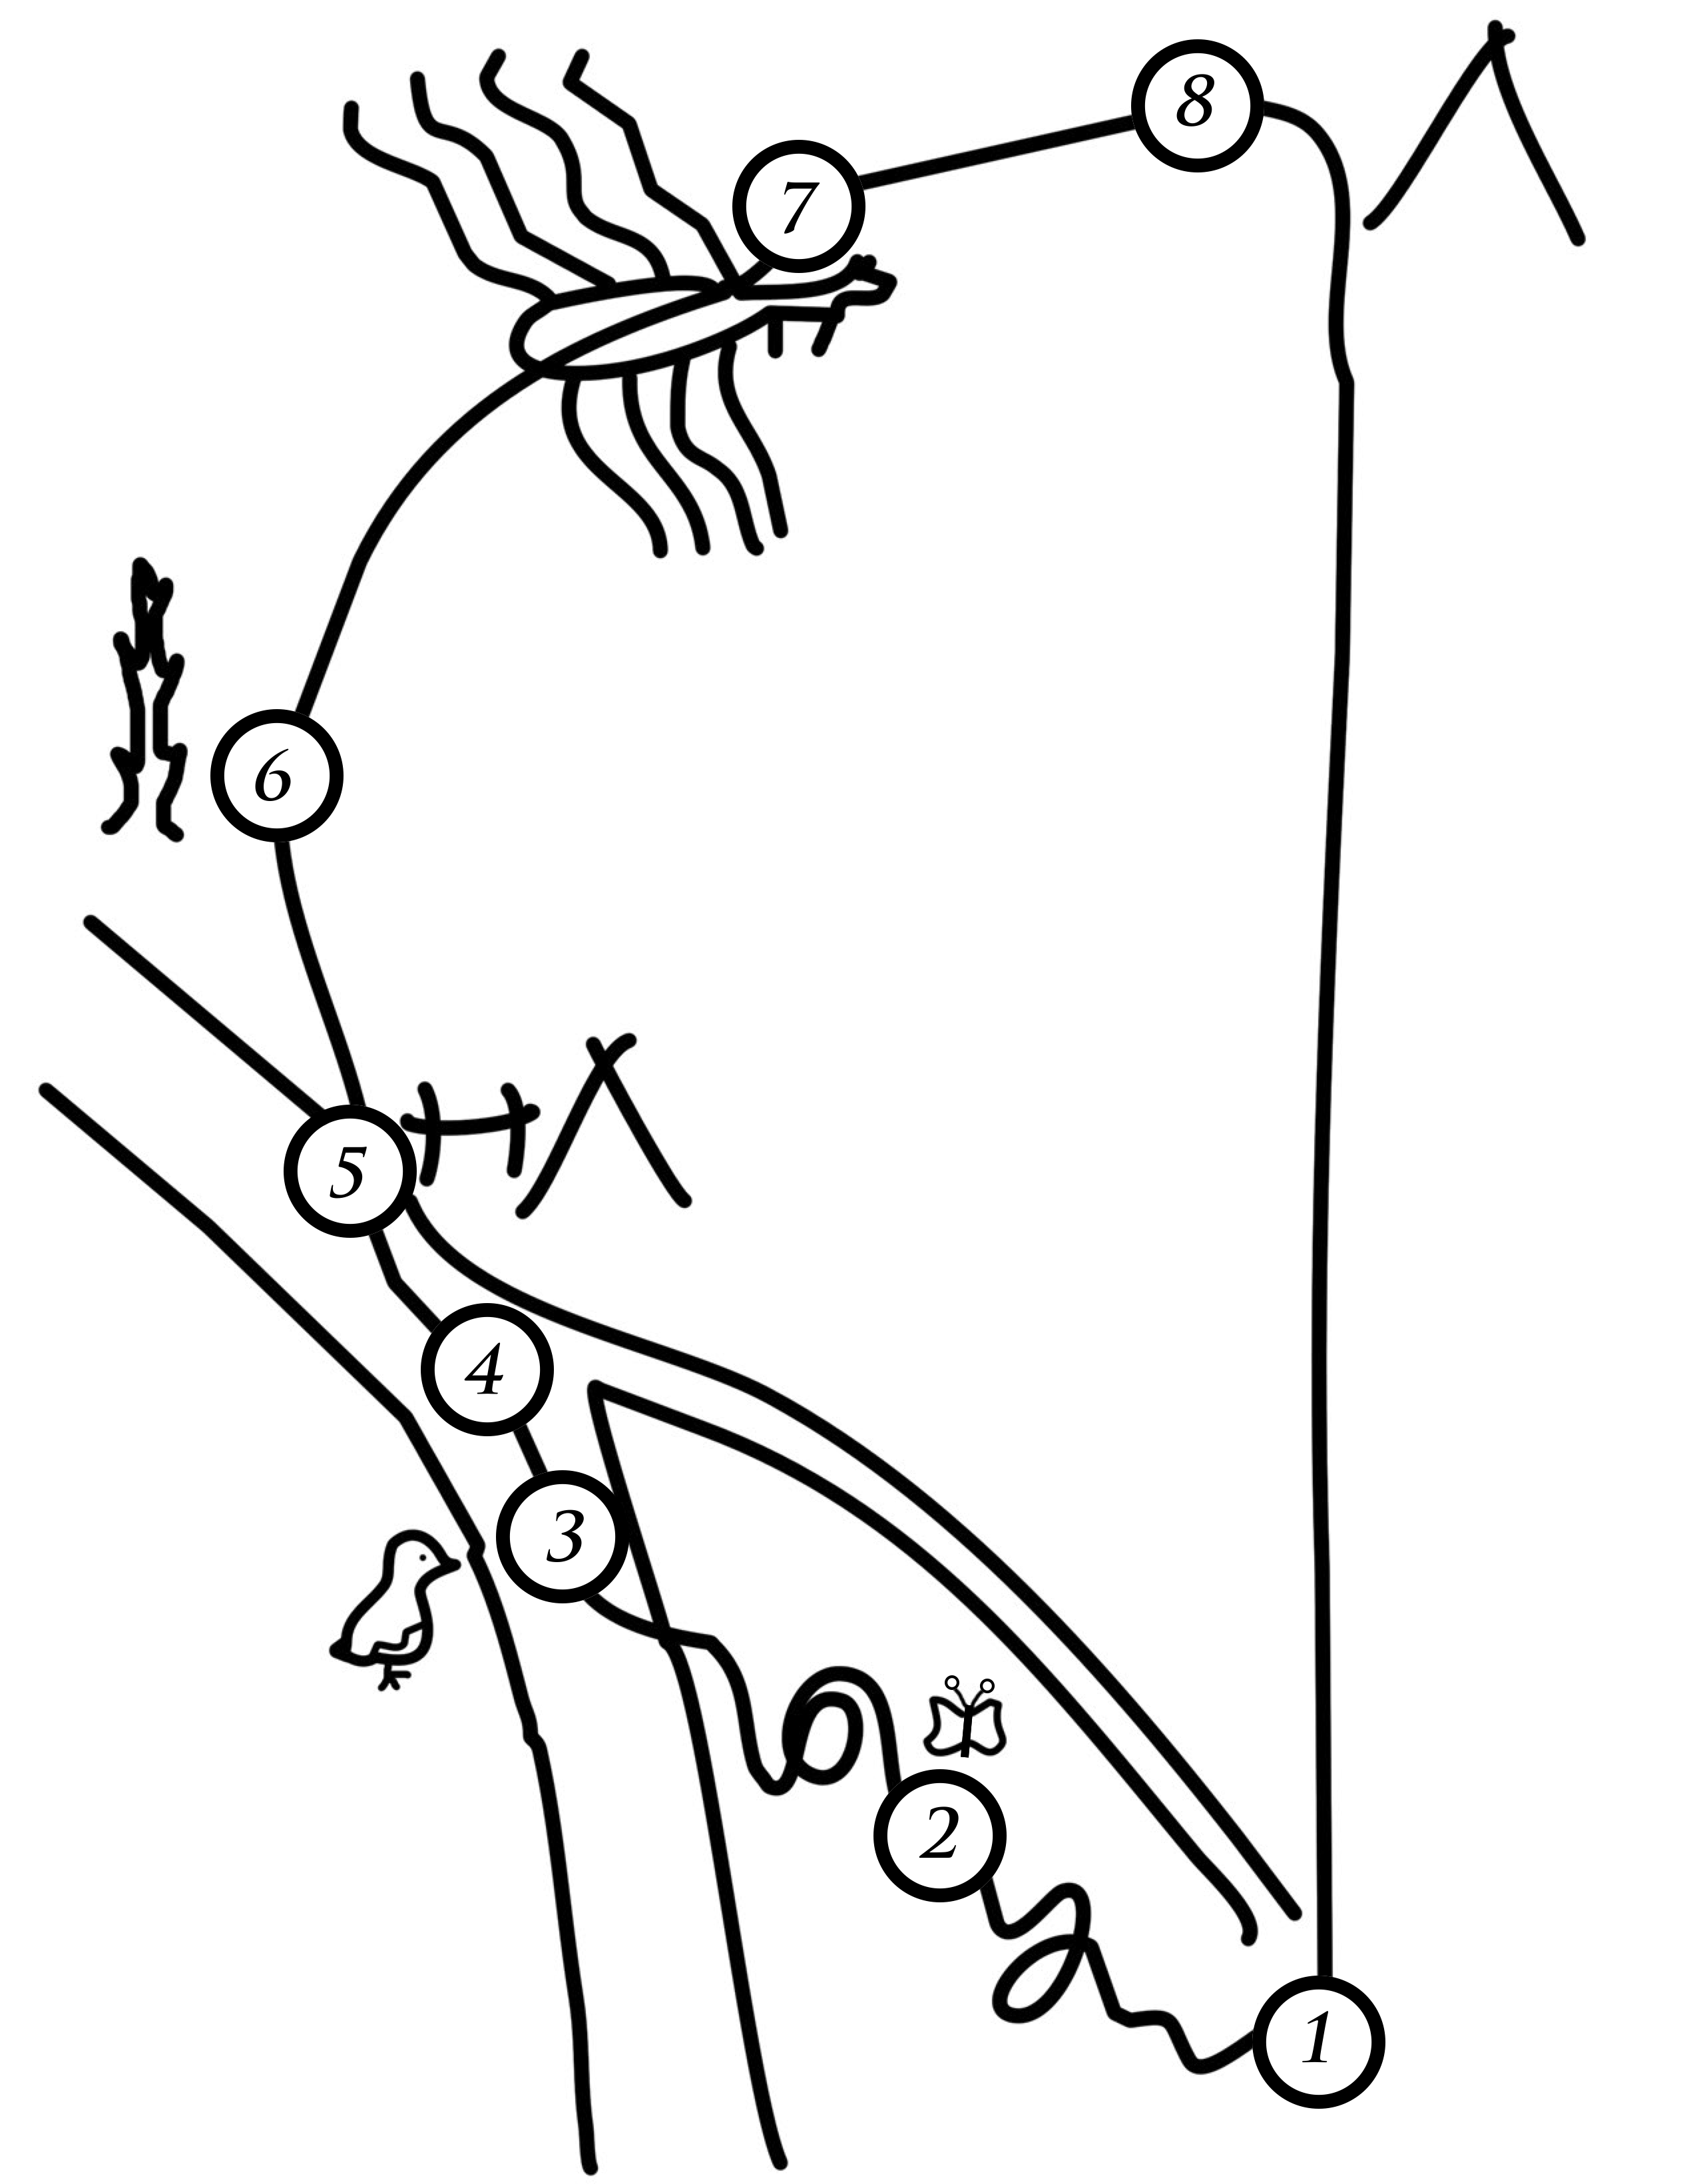
\includegraphics[width=0.7\textwidth]{figures/brucks-fig1} %twogirlsmap
    \caption{Episodes of the Butterfly Story}
    \label{brucks:fig:epmap}
\end{figure}

\begin{quote}
(1) Two Girls follow a Butterfly that leads them astray (2), and they get lost. As they walk upland, they encounter a Chickadee (3) who tells them about a crossroads (4) where they have the choice between two trails. Chickadee advises the Girls to follow the narrow trail, which will lead them home, but does not say what awaits if they follow the wide trail. The Younger Sister wants to take Chickadee's advice, but the Older Sister insists on them taking the wide trail. They then encounter an Old Man (the Devil) living all by himself (5). There are many signs that he is an evil person; for example he has a drying rack with dog skulls on it, or he serves the Girls soup with eyes in it. The Older Sister ignores these warning signs and sleeps with him; she is raped by him with a red-hot iron penis and dies. The Younger Sister remains wakeful through the night and watches her Sister's murder. In the morning, she escapes with the help of a Tree Stump (6) and runs away to a river that she crosses on the tail of a Fox (7). She finally arrives at the tent of an Old Lady (8) who is variously identified as {\em Saa Wunąą} `the Mother of the Sun' or {\em Tsǫǫ Kelahdzeey} `Grandmother Spider'. When the Devil catches up with her there, the Old Lady kills him by melting his flesh with her gaze. The Younger Sister turns his bones and organs into edible plants. She stays with the Old Lady for a while, but is so homesick that she descends through a hole between the worlds to her family, using a rope that she made from moose sinew over a period of many days. When she returns, it begins to snow, a sign that the Old Lady has been killed by her sons.
\end{quote}

In his introduction to Mrs. Mary Tyone's version of this story, James Kari notes that it may be ``regarded as a cautionary tale for young girls'' \citep[23]{TyoneM1996}. Young people are encouraged to follow the `narrow' trail of morality. The Older Sister's insistence on taking the wide trail is punished by rape and death; the Younger Sister only narrowly escapes this fate. (While this piece of advice smacks strongly of Christianity, it is present in all recorded versions of the story, suggesting that it pre-dates missionary influences.) Also important is listening to one's elders; the Older Sister ignores Chickadee's advice and gets killed while the Younger Sister listens and survives. Another lesson is to pay attention, both geographically (to one's surroundings) and morally (to one's behavior).\footnote{\citet[468]{GuedonMF2005} arrives at different lessons contained in this story: ``Ne vous éloignez pas du groupe, ne parlez aux étrangers, faites bien attention à ce qui se passe autour de vous.'' (Don't go away from the group, don't talk to strangers, pay close attention to what happens around you. Translation by the authors.)}

The story follows a circular trajectory, leading the Girls first up and away from their parents into another world, then through a mythological landscape, and finally back down to their parents. The audience is able to follow this trajectory by paying attention to the directional adverbs so pervasive in Northern Athabascan storytelling \citep{KariJ2010, KariJ2011}, which create a `virtual landscape' of the events. As other authors have noted of Athabascan storytelling, directionals, in addition to place names, enable listeners to follow the events of the story ``like a map'' \citep[62]{CruikshankJ1990, MoorePTlenD2007}. This is allowed by the deictic nature of directionals which create a point of view from which to view events which is ``just like being there'' \citep[58]{MooreP2002}. Busch reiterates this view for the Gwich'in saying that listeners can ``form very clear images of the location of actions and the direction of movement being described'' \citet[1]{BuschJ2000}\footnote{For more on the role of directionals in creating narrative space in Upper Tanana stories see \citet{BrucksC2015}.}.

What is striking about this particular narrative is that the Girls lose their way; first in the physical world after following the Butterfly and then in the spiritual world during their encounter with the Old Man. We contrast the serious reduction of directional use in the episodes involving the morally deficient Old Man against the more robust use of directionals—and other spatial descriptions—in the episodes involving the the other (helpful) characters. As we will show in this paper, the storytellers skillfully convey a sense of disorientation—both moral and spatial—by severely curtailing their use of directional adverbs during the episodes involving the Old Man.

The explicit sexual content of the Butterfly story, and in particular the many deviations from what the Upper Tanana consider normal sexuality, is one of the most troubling aspects of this story. Respecting the wishes of several Elders we work with, we will touch on these issues only briefly throughout the paper. We did however make the decision to include them in the discussion, since the deep immorality of the Devil will not otherwise become clear.

This paper is structured as follows. In § \ref{brucks:section:background}, we provide some background information on the Upper Tanana language and on the four versions of the story discussed here. We also give a brief introduction to directional adverbs in Upper Tanana. In § \ref{brucks:section:losing-direction}, we look at what the use of directional adverbs reveals about the Girls' travel through geographic space before turning to the moral disorientation caused by the Devil in § \ref{brucks:section:losing-moral-direction}. We show that the moral disorientation is reflected in the use of directional adverbs and (verbal) prefixes in § \ref{brucks:section:discussion}.

\section{Background}
\label{brucks:section:background}

Upper Tanana is an Athabascan language spoken in eastern interior Alaska and the western Yukon Territory. \citet{MinouraN1994} distinguishes five dialects: Beaver Creek (in the Yukon), Scottie Creek, Northway, Tetlin and Nabesna. Documentation of Upper Tanana was done by SIL linguist Paul Milanowski, resulting in a partial bible translation \citep{MilanowskiPJohnA1966, MilanowskiPJohnA1972} and a Junior Dictionary \citep{MilanowskiPJimersonS1975, MilanowskiPJohnA1979}. James Kari contributed by collecting place names \citep{KariJ1997UTmap}, doing lexicographical work \citep{KariJ1997stem}, and editing a story collection \citep{TyoneM1996}. Several linguistic articles on Upper Tanana can be found in \citet{MinouraN1994, MinouraN1997, TuttleSLovickONunez-OrtizI2011}, and \citet{LovickO2012a-metaphor, LovickO2012b-genre}.

Today, Upper Tanana is severely endangered. There are only 50–90 remaining speakers, and most of them are elderly. There are no more speakers of the Scottie Creek dialect (documented primarily by James Kari) and only a 2–3 speakers of the Nabesna dialect. The Tetlin dialect is also severely endangered with fewer than 10 speakers, while the Northway and Beaver Creek dialects are both still relatively healthy with estimates of more than 20 speakers per dialect.

The observations in this paper are drawn from four tellings of the Butterfly Story. The oldest of these is by the late Mrs. Mary Tyone. It was recorded by James Kari in November 1992; some corrections were made in 1994 before its publication in \citet[23–33]{TyoneM1996}. Mrs. Tyone was a speaker of the Scottie Creek dialect.

The second version was told by the late Mrs. Cora H. David of Tetlin in April 2008 and was recorded by Olga Lovick; it is published in \citet[118–133]{DavidC2011}. Mrs. David was a speaker of the Tetlin dialect.

The third version was told jointly by the late Mrs. Darlene Northway of Northway and Mrs. Jeanie Sanford of Mentasta; it too was recorded by Olga Lovick. The speakers took turns telling the story. Mrs. Northway was a speaker of the Northway dialect; Mrs. Sanford is a speaker of the Beaver Creek dialect.

The fourth version was told by Mr. Roy H. David Sr. (the husband of Mrs. David) of Tetlin in November 2014 and was recorded by Caleb Brucks and Olga Lovick. Mr. David is a speaker of the Tetlin dialect.

Not surprisingly, the two stories told by Mrs. and Mr. David (both from Tetlin) are very similar; Mr. David however explicitly states that he learned this story from (among other people) his mother-in-law—Mrs. David's mother. Similarly, Mrs. Northway's and Sanford's telling is in many places quite similar to Mrs. Tyone's—both of them credited Mrs. Tyone as one of their teachers.

The version by Mrs. Tyone was transcribed and translated by James Kari and Mrs. Tyone; the other versions by Olga Lovick and Caleb Brucks with the help of several speakers of Upper Tanana. While the orthography employed by us follows largely that devised by James Kari as represented in \citet[xi-xvi]{TyoneM1996}, there are some differences. Some of these have to do with dialect; to give an example, the Tetlin dialect does not distinguish the vowels written as <a> and <ä>, so both are represented as <a> in that dialect (see \citealp{TuttleSLovickONunez-OrtizI2011} for more detail); also, in the Northway and Tetlin dialects, the diphtong <įǫ>, which still exists in the eastern dialects, has merged with <ǫǫ> and <iu> with <uu> \citep{LovickO2011}. Other differences may represent variant pronunciations or analyses; for example, Kari writes the vowel of the third person plural object prefix usually long as {\em huu}-, while Lovick tends to write it short as {\em hu}-. For the purposes of the present paper, the spelling of Tyone (1996) is retained in examples taken from that book. The original free translations are also retained here; word glosses have been added by the authors.

The class of adverbs commonly referred to as directionals is a major contributor to spatial description in the Upper Tanana language. Directional forms are made up of three parts: one of nine stems which denote an angle of direction, one of four suffixes (Allative `towards', Ablative `from', Punctual `at a point', Areal `in a general area'), and a prefix of relative distance. The stems and suffixes are synchronically fused so that the stem-suffix combination is now considered a complex stem in Upper Tanana \citep[591]{LeerJ1989}. Prefixes are common but not obligatory. The Proto-Athabascan reconstructions in Table \ref{brucks:table:dir-adv} are taken from \citet[616]{LeerJ1989}.

\begin{table}
\caption{Directional stems in Proto-Athabascan and Upper Tanana}
\label{brucks:table:dir-adv}
\begin{tabular}{ l | l l l l l }
English & Proto-Athabascan & Upper Tanana \\
 & & ALL & ABL & PUNC & AREAL \\ \hline
‘up above’ & *deG & degn’ & dǫǫ {\em or} doo & daa & dogn \\
‘down below’ & *yeG, yex & shyign' & shyǫǫ & shyiit & shyuugn \\
‘upstream’ & *niʔ & ne' & nǫǫ {\em or} noo & noot & nuugn \\
‘downstream’ & *daʔ & da' & dǫǫ {\em or} doo & daat & duugn \\
‘upland’ & *neG & negn' & nǫǫ {\em or} noo & niit & nogn ~ nuugn \\
‘downland’ & *cenʔ & tthän' & tthǫǫ & tthiit & tthuugn \\
‘ahead’ & *nәsd & noo' {\em or} noo & ? & ? & noogn \\
‘across’ & *ŋaˑnʔ & naan' & nǫǫ & naat & nuugn \\
‘away’ & *ʔαnʔ & ’än' & ’ǫǫ & ’aat & ’ogn {\em or} ’oogn \\
\end{tabular}
\end{table}

The Upper Tanana adverbial directional system is anchored to the main waterway of the area. The largest and most important river of the area, the Tanana, begins at the confluence of the Chisana and Nabesna rivers near Northway and runs a little north of west until it flows into the Yukon several hundred miles away. Five of the nine directional stems directly reference the Tanana creating a four-way ``intermediate absolute landmark" system (\citealp[90-91]{LevinsonS2003}, \citealp[129]{KariJ2010}). This subset of the directional adverbs often referred to as `riverine directionals' include the opposing pairs of {\em negn'} `upland' vs. {\em tthän'} `downland',  {\em ne'} `upriver' vs. {\em da'} `downriver', and {\em naan'} `across', which is its own opposite \citep[576]{LeerJ1989}. They match the general east to west flow of the river but are also largely abstracted. As such, the directionals can be used when well away from the Tanana river if still in the same region. For example,  {\em negn'} `upland' can be used when travelling upstream on the Nabesna as it is `upland' viewed from the Tanana.

In addition to the regional uses of the riverine directionals, directionals can be used in local settings to refer to the upriver direction of a minor tributary or to point across local landmarks such as lakes or treeless flats. The remaining (non-riverine) directionals are generally used in this local manner as well. {\em Degn'} `up (vertically)' and {\em shyign'} `down (vertically)' are used in settings like `up (a tree)' and or `down (on the floor)' as well as `uphill' or `downhill' with no (horizontal) direction specified. The remaining stems are vague in their directional content. The `ahead' {\em noo'} stem does not specify any set direction though it is often used when moving out in to open areas and {\em 'än} is even more devoid of spatial content with a general `away, outside' meaning. The directional stems are also extended to a number of other settings—such as the interior of houses (see \citealp[131]{KariJ2010} for more examples). While the use of directionals likely have a historical origin in the normal orientation of houses to the river (see \citealp{FortescueM2011} and \citealp[602]{LeerJ1989}), the directional stems in Upper Tanana are removed from their direction-bearing content and lexicalized as discrete forms, such as {\em ne'} `side of the house' or `rear, behind (gun, animal, person, etc.)' for instance. A clear example of this is found with the {\em 'än} `away' stem which takes the meaning `outside (the house)' and is the opposite of {\em noo'} `inside, toward the center (historically: the fire)'. In these cases, then, the directional stems are more than ample to describe the `microcosm' \citep[7]{FortescueM2011} inside the house but are of a different type from the directionals used in reference to rivers or major landmarks.

Upper Tanana also has a rich inventory of adverbial verb prefixes. These are part of what \citet[28]{KariJ1979} terms `aspectual derivational strings', which are discontinuous morphemes with clear semantic content (e.g. {\em ske}- `across a body of water' or {\em dzi-na}- `down over an edge') that apply productively to a number of verbs. A substantial subset of these prefix strings is used to describe motion through space, and derives a number of motion verbs. While our focus in this paper lies on the use of directional adverbs, we will occasionally make reference to directional prefix strings where they serve to clarify the motion described in the narrative.

\section{Losing one's place}
\label{brucks:section:losing-direction}

The story begins with the Two Girls chasing a Butterfly. They then become lost and at some point leave `our' world behind and enter a world on top of the sky. It is intriguing, though, that the versions differ in when exactly this transition between worlds takes place. In Mrs. Tyone's version, the transition happens at the very beginning of the story as demonstrated in (\ref{brucks:tyone-transition-to}).\footnote{The following abbreviations are used in this paper: CT—contrastive topic, \textsc{foc}—focus, PL—plural.}

\begin{exe}
\ex Transition into the world above the sky (Mrs. Tyone) \label{brucks:tyone-transition-to}
\begin{xlist}

\ex \gll Dziin uudih Laalil nahnetdik.  \\
 day all butterfly {they kept following around} \\
\glt `All day long they followed butterflies.' \\

\ex \gll Ishyiyit t'eey t'axo Laalil huu'eh keenän'ii'ąą.  \\
 then even finally butterfly {with them} {it took the world up} \\
\glt `And then, all of a sudden, Butterfly took them up to another world.' \\

\ex \gll Yaat'agn tah huu'eh nän' ninii'ąą.  \\
 {through sky} among with them earth {it took up} \\
\glt `It took them through the sky into another world.'  \\

\ex \gll Ishyit tąy haadäl eh huu' nduu {huu'eh huushyaak} ts'ą̈'.  \\
 there trail {they were going} and ? somewhere {they got lost} and \\
\glt `They were going on the trail there, and they got lost somewhere.' \\
\end{xlist}
\end{exe}

In the version by Mrs. David, given in (\ref{brucks:davidc-transition-to}), the Girls cross into another world very early as well. Note that in (\ref{brucks:davidc-transition-to}a-b), the Girls' mother explicitly warns them not to follow the Butterfly.

\begin{exe}
\ex Transition into the world above the sky (Mrs. David) \label{brucks:davidc-transition-to}
\begin{xlist}

\ex \gll Hunąą huts'ą' ehsał nts'ą': ``Ena'! Sǫ'!''  \\
 {their mother} {to them} hollered and no don't \\
\glt `Their mother hollered at them: ``No! Don't!'' ' \\

\ex \gll ``Laalil natnatdagn stanuhtaałeeł nt'eh,'' hu'ehnih.  \\
 butterfly {you, following} {he will take you away} certainly {she told them} \\
\glt ` ``If you follow the Butterfly, he'll take you away for sure,'' she said to them.' \\

\ex \gll T'oot'eey k'at'eey hiidiitth'agn nts'ą' Laalil \textbf{nahdogn} ch'idanh keey k'it tah kehu'įįdlah.  \\
 but not {they didn't listen to her} and butterfly up different village on among {it took them} \\
\glt `But they did not listen to her, and the Butterfly took them up to a different world.' \\

\ex \gll Eł hu'ihuushyaak.  \\
 and {they got lost} \\
\glt `And they got lost.' \\
\end{xlist}
\end{exe}

In both versions, following the Butterfly is the direct cause of the Girls' getting lost. In (\ref{brucks:tyone-transition-to}), the Butterfly takes the earth, {\em nän'}, as a single round object through the sky; the Girls are taken together with the earth. In Mrs. David's version, the Butterfly takes a plural object—the Girls—up into a different `village': a different world. The notion of `up' in (\ref{brucks:davidc-transition-to}) is expressed in several ways: by the directional adverb {\em nahdogn} `Area above', by the postposition {\em k'it} `on top', and finally by the prefix string {\em ke}- `up, against' in the verb form {\em kehu'įįdlah} `it took them', which also occurs in themes describing other types of vertical motion, e.g. climbing a tree.

In the version told by Mrs. Northway and Mrs. Sanford, the Girls simply get lost; the narrators do not explicitly state at which point the transition into the other world takes place. In the version told by Mr. David, crossing into the world above the sky seems to happen in stages. The Butterfly leads the Girls away in the uphill direction where they get lost.

\begin{exe}
\ex Transition into the world above the sky (Mr. David)\label{brucks:davidr-transition-to}
\begin{xlist}

\ex \gll Hǫǫ tay' hidetnii huch'a tah niłk'ineht'ah niłk'ineht'ah huch'a.  \\
 thus again {they grabbed it} {from them} among {it fluttered around} {it fluttered around} {from them} \\
\glt `Again they tried to grab it but it fluttered away from them, it fluttered away from them.' \\

\ex \gll Niłk'ineht'ah huch'a nahiitnetdak  \\
 {it fluttered around} {from them} {they started following it}\\
\glt `It fluttered away from them and they started following it.' \\

\gll Tąy nts'ą' t'eey stahuunįįdlah, \textbf{deg'} uudih. \\
 trail to even {he took them away} {up vertically} {totally} \\
\glt `He took them away to a trail, all the way up.' \\

\ex \gll Ddhał taag ch'ale',  ddhał taag tah, \textbf{deg'} tah, \textbf{deg'} tah hu'aałeeł ndee hiits'ihetniign.  \\
 mountain three \textsc{foc} mountain three among {up vertically} among {up vertically} among {it was taking them} {where to} {they didn't know}  \\
\glt `Over three mountains, over three mountains, up and up it took them, they did not know where to.'\\
\end{xlist}
\end{exe}

In subsequent conversations, Mr. David clarified that while the Girls have left `our' world behind in crossing the mountains, they have not yet entered the world above the sky. The Younger Sister arrives in the place above the sky only after she has crossed the river with the help of Fox. At that point of the story, the Older Sister has been killed and the Younger Sister is running from the Devil. If we understand Mr. David correctly, then the Girls' journey to another world is very gradual; they leave their own world while chasing the Butterfly, but their crossing between worlds is incomplete until the Younger Sister comes to the river (Authors' fieldnotes, November 20, 2014).

At first glance, it is surprising that the narrators disagree about the exact place of the crossing. But as \citet[470f.]{GuedonMF2005} convincingly shows, the boundaries between the two worlds are not fixed in Upper Tanana cosmology: any place can serve as entry point, and many animals can serve as guides from one world into the other. Moreover, the landscape of the world above the sky so closely resembles ours—with hills, trees, flats, and rivers—that it is not surprising that at first, the Girls do not notice that they have come to a different place, with different rules and different dangers. Here as well as elsewhere, though, there are ``good'' and ``bad'' roads to travel (cf. \citet[473]{GuedonMF2005}, and the Girls will have to figure out which is which.

Soon after getting lost, the Two Girls reach a crossroads. A Chickadee advises the Girls to take the narrow trail and explicitly warns them off the wide one. This passage, as told by Mrs. David, is given in (\ref{brucks:cora-chick}); the versions by Mrs. Tyone and Mr. David are very similar to this. In the version told by Mrs. Northway and Mrs. Sanford, the Girls have to decide on their way without Chickadee's help.

\begin{exe}
\ex Chickadee's advice (Mrs. David) \label{brucks:cora-chick}
\gll {Ay eł} Ts'igąąk: ``Tąy ts'eegn k'e ahdeeł, sǫ' tąy teeł k'e ahdeel,'' hu'ehnih. \\
 and Chickadee trail narrow on {you go} don't trail side on {you don't go} {he told them} \\
\glt `And Chickadee said to them: ``Go on the narrow trail, don't go on the wide trail!'' \\
\end{exe}

In all versions, the Younger Sister wants to go onto the narrow trail (which would have led them back home), but the Older Sister fights her physically and drags her onto the wide trail (\ref{brucks:decision-dn-js}):

\begin{exe}
\ex Making the decision (Mrs. Northway and Sanford) \label{brucks:decision-dn-js}
\begin{xlist}

\ex \gll Didia' tthiits'äl' uuniik tl'aan \textbf{nahdegn'} tah ch'itsąą tąy \textbf{degn'} tah didia' ditthiixa' eh aałiu.  \\
 {her younger sister} hair {she grabbed} and {up vertically} among different trail {up vertically} among {her younger sister} {her hair} with {she dragged} \\
\glt `She grabbed her Younger Sister's hair and up there onto the other trail she dragged her Younger Sister by her hair.' \\

\ex \gll Ay tl'aan \textbf{hohdegn'} hihteedeel eh \textbf{nah'ogn} łįį tthi' dineh tthi' eetah dahdzäl k'it da'eedlay huunehttheh.  \\
 and then {up vertically} {they started} and {out there} dog skulls man skulls {among them} {drying rack} on {they were up} {they were barking} \\
\glt `And then they began to walk uphill and out there there were dog skulls and human skulls up on the drying rack and they were barking.'   \\
\end{xlist}
\end{exe}

Even though the Girls have left our world behind, the use of directionals continues up to the point where they arrive at the Old Man's camp. Despite having chosen the bad trail, they have retained enough of their sense of orientation to keep going. But the barking skulls on the drying rack are the first indication that something is very, very wrong. As it turns out, the Girls now are not just lost spatially, but they are also in a place where their moral sense of direction will be severely challenged.

\section{Losing one's moral sense of direction}
\label{brucks:section:losing-moral-direction}

The episode where the Two Girls first encounter the Devil is deeply disturbing. The Girls have entered a place where unnatural and immoral activities take place, which challenges their ability to distinguish right from wrong. This episode diverges from the previous sections by introducing the antagonist of the narrative, the Old Man or Devil, who is a morally disorienting force. He encourages the Girls to commit morally questionable acts and seeks to keep the Girls from finding their way home---essentially he aims to keep them ``lost''.

The encounter begins with the Two Girls first meeting with the Devil. In three of the four narratives (Mrs. David's story excluded) the Girls' arrival at his camp is greeted by the barking of dogs. However, the Girls quickly learn that the barking is coming not from dogs but from their parts left on a drying rack.

Mrs. Sanford and Northway's version is the only one where the dogs (their skulls) share the drying rack with human remains (see (\ref{brucks:decision-dn-js}f) above). No less odd, however, are the barking split carcasses of dogs in Mrs. Tyone's story (\ref{brucks:tyone-barking-dogs}) or the barking eyes in Mr. David's version (\ref{brucks:rdavid-barking-dogs}e).

\begin{exe}
\ex Coming in to the Devil's camp (Mrs. Tyone) \label{brucks:tyone-barking-dogs}
\begin{xlist}

\ex \gll \textbf{Xahdogn'} dahdzäł k'it łįį elk'aagn naat da'eedlay.   \\
 {up above} {drying rack} on dog split across {they lie}  \\
\glt `Up above on the rack were split dog carcasses.' \\

\ex \gll  Ay łįį elk'aagn gąy in t'eey ttheehihdelxoh ay'eh ishyiit.  \\
  and dog split dry PL even {they are barking} and there \\
\glt `And those dry dog carcasses were barking right there' \\
\end{xlist}
\end{exe}

\begin{exe}
\ex Coming in to the Devil's camp (Mr. David) \label{brucks:rdavid-barking-dogs}
\begin{xlist}

\ex \gll ``{Dii xa} ndee ts'anh ch'ale łįį needehtthay?''   \\
 why where from \textsc{foc} dog {barking at us}  \\
\glt ` ``Why, where are the dogs barking at us?'' ' \\

\ex \gll ``K'at'eey łįį nak'ąy,'' nih.  \\
 not dogs {I don't see} {she said}  \\
\glt ` ``I don't see any dogs,'' she said.' \\

\ex \gll  \textbf{Nahdegn'} dahdzal k'it uneh'ąy eh tah tth'an' uuł.  \\
  {up vertically} {drying rack} on {she looked} and among bone skeleton \\
\glt `She looked up at the drying rack and [there were] bones, skeletons.' \\

\ex \gll  Ay ch'a Ts'ant'ay łįį atnag.   \\
  and \textsc{foc} Devil dog {he eats} \\
\glt `And this was the Devil, he eats dogs.' \\

\ex \gll  Ay ch'ale unaag' ch'ale hunehtthay.  \\
  And \textsc{foc} {their eyes} \textsc{foc} {barking at them} \\
\glt `And it was their eyes barking at them.' \\
\end{xlist}
\end{exe}

Barking pieces of dead dogs is certainly an odd event and thus strongly signal that the Girls have entered an entirely different world. Importantly, it is also an indication of the immorality of the Old Man. Eating dogs is strictly taboo in the Upper Tanana area as it is among other Athabascan groups. \citet[162]{McKennanR1959} states that the ``Upper Tanana hold the dog in peculiar reverence, and they will neither kill nor eat it although they have no rationalized explanation for this taboo''. \citet{NelsonR1983}, in his discussion of Koyukon relationships with animals, emphasizes the usefulness of dogs as pack and guard animals, but finds their role as companions the most important; dogs have a privileged relationship with humans as their only domesticated animal. Thus, though killing dogs is not taboo when they have outlived their usefulness, eating them definitely is, and \citet[191]{NelsonR1983} suggests that this is because it ``is perhaps akin to cannibalism, given their closeness to humans''. This closeness is clear in that dog owners are referred to as their dog's {\em bitsiya} `grandfather' and that dogs are the only animal to share the plural morpheme {\em -kka} with humans. Though the Upper Tanana neither refer to dogs as their grandchildren or share a human plural with dogs (although dogs are more commonly pluralized than other animals) they share a close relationship with dogs unequaled by any other animal (even today the dog is the only animal kept as a pet) and thus the repulsion to eating them remains strong.

The reverence for dogs is mixed with a certain level of unease with their spiritual power. For example, Koyukon people traditionally did not allow dogs to live in the house as it would make the children behave like dogs which presumably ``means eating unclean things, acting wild and unruly, being half animal'' \citep[191]{NelsonR1983}. A similar fear of the ``unclean'' spirit of dogs is seen in the Upper Tanana taboos which restrict dogs from eating the heads of large game or carcasses of fur bearing animals as it will remove the hunter's or trapper's luck \citep[168]{McKennanR1959}. Similarly, if dogs find the placenta of a newborn child the woman will bear no more children \citep[167]{McKennanR1959}. Dogs are both creatures close to humans as well as unclean and dangerous to them and thus the Devil is committing a doubly abhorrent act by eating them.

However, eating dogs also shows that the Old Man is a different type of being than the Girls—a type of being which finds eating dogs (and humans perhaps) as normal as eating white fish or moose is for the Upper Tanana. That is, this event illustrates the perspectival \citep{ViveirosDeCastroE1998} outlook common in the cosmology and narratives of Alaskan Athabaskans. (While the argument for a perspectival view was originally put forward by Viveiros de Castro based on Amazonian groups, similar arguments have been made for North American groups by \citet{IngoldT2000} for the Ojibwa and \citet{NadasdyP2003} for the Kluane.) In the current narrative, then, the fact that the Old Man eats dogs, something that real people would never do, shows that he is a different type of being: a type of being who sees killing, drying, and eating dogs the same way humans see doing this to moose or caribou.

The version told by Mrs. David does not have barking dog parts at the beginning of the two Girls' encounter with the Devil. Instead, the eating of dogs enters the narrative in a much more direct manner: the Old Man serves the Two Girls a soup with dog eyes in it.

\begin{exe}
\ex Eating dog eyes (Mrs. David) \label{brucks:cdavid-dogs-eyes}
\begin{xlist}

\ex \gll Ch'idia' hashyiign tuuthał shyiit huneh'ąy eł łiign naagn' dii naagn' le' ushyiit natatdiiłek.   \\
 {younger sister} down soup in {she looked} and dog eyes what eyes UNCERT {in it} {were floating} \\
\glt `The Younger Sister looked down into the soup and dogs' eyes and I don't know what sort of eyes were floating in it. ' \\

\ex \gll Eł: ``K'at'eey tih'aal!'' yuunih nts'ą' dushyiign t'eey naatehtl'iit dą' ch'itay nahtak.  \\
 and not {I won't eat it} {she thought} and down even {she spilled} when {old man} {looked away}  \\
\glt `And, ``I'm not going to eat it!'' she thought and she spilled it when the Old Man wasn't looking.' \\

\ex \gll  Ch'aadeh du' naye'aał.  \\
 {older sister} CT {ate it} \\
\glt `The Older Sister however ate it.' \\
\end{xlist}
\end{exe}

Eating the dogs' eyes is problematic in a number of ways. Eyes in themselves are dangerous and children should never touch them as it will cause ``nightmares, cramps, or something worse'' \citep[177]{GuedonM1974}. Also, by ingesting certain foods, one acquires some of the properties of this food, both positive and negative \citep[233]{NelsonR1983}. Young girls who just had their first period may not eat ripe berries, as that is believed to cause excessive bleeding \citep[21]{TyoneM1996}. Young children may not eat moose meat because young moose are so awkward; instead, children are fed caribou meat since caribou are up on their feet just minutes after their birth \citep{DavidCforthc}. Through her action, the Older Sister acquires one of the most salient trait of dogs: inattentiveness \citep[104, 110]{LovickO2012a-metaphor}. Lovick cites the expression {\em Łįį k'eh uht'iin ahłįį} `You guys are like dog people', which according to Mrs. David was used frequently by her own mother when admonishing her children to pay attention and listen to her Elders. Dog people, apparently, do not pay attention and do not listen to advice. By eating dog, the Older Sister becomes more dog-like, less human.

This has disastrous consequences for the Older Sister. She loses her ability to see the world the way a human does it, and thus to distinguish right from wrong; she now views the world in the immoral way of the Devil. She next declares her intention to sleep with the Devil, who recognizes her as an easy victim and kills her by raping her with a red-hot iron pole. The Younger Sister, who has surreptitiously refused to partake of the dogs' eyes, retains her ability to see clearly, and thus escapes the Devil. She has retained her sense of self as a human being (see also \citealp[470]{GuedonMF2005}).\footnote{This interpretation of the significance of eating eyes was confirmed in a conversation with Mrs. and Mr. David on May 17, 2013.}

The episode where the Devil rapes and kills the Older Sister abounds in all variants with verb themes having to do with seeing. In a stretch of text between 4 (Mrs. David) and 25 (Mr. David) lines long, a total of nineteen `seeing' verbs belonging to seven different verb themes is used. This emphasis on seeing stresses the watchfulness of the Younger Sister, especially as compared to the inattentiveness of the Older Sister. Even more importantly, reliance on the sense of sight distinguishes humans from many other animals that rely more on their sense of sound or smell. The Old Man in this story is different, non-human, in that he uses his sense of smell to track down the Girl, just like a dog would do. (The Upper Tanana used dogs frequently as hunting companions and were thus certainly aware of that animal's keen sense of smell.) Crucially, the Devil's following the Younger Sister's scent trail is a feature of all four variants of this story.

At this point of the story, the Older Sister has made several crucial mistakes. She has left home—and presumably her chores—behind to chase after a Butterfly, and she has taken the wrong turn at the crossroads. At the Old Man's camp, she ignores all the warning signs. In both Mr. and Mrs. David's versions, the Old Man is identified as a bad and lying individual from the outset, who pretends to follow Athabascan protocol of welcoming unexpected guests, feeding them and offering a safe place to stay \citep[140]{GuedonM1974}. But the food he offers is unclean, and the place he offers is anything but safe. In these two versions, the Older Sister's lack of judgment manifests itself through the—ordinarily innocuous—act of falling asleep. By abandoning her vigilance, she eventually causes her own death.

In the versions told by Mrs. Tyone and by Mrs. Northway and Sanford, the Old Man does not live entirely alone; opposite him, an Old Lady is staying (in the version told by Mrs. Northway and Mrs. Sanford, this Old Lady is identified as {\em Tsǫǫ Kelahdzeey} `Grandmother Spider'; in Mrs. Tyone's version, the Old Lady remains unnamed). In this version, the Older Sister's loss of moral direction is quite a bit more blatant:

\begin{exe}
\ex Spending the night (Mrs. Northway and Mrs. Sanford) (UTOLAF10Jul0202) \label{brucks:sleep-with}
\begin{xlist}

\ex \gll Ay tl'aan {ts'exeh gaay} ishyiit du' Tsǫǫ K'elahdzeey xa nihnįįdeel eh.  \\
 and then Girl there CT Grandmother Spider for {they arrived} and \\
\glt `And then the Girls went to Grandmother Spider.' \\

\ex \gll Ch'idia' du: ``Stsǫǫ eh tihteeł!''  \\
 {younger sister} CT {my grandmother} with {I will sleep} \\
\glt `The Younger Sister [said]: ``I will sleep with my grandmother!'' ' \\

\ex \gll Ch'aadeh du': ``Stsay eh tatihteeł!''  \\
 {older sister} CT {my grandfather} with {I will sleep} \\
\glt `The Older Sister [said]: ``I will sleep with my grandfather!'' ' \\

\ex \gll Maa hǫǫsǫǫ ditsay eh teete'.  \\
 {for her} good {her own grandfather} with {she will sleep} \\
\glt `She is happy that she is about to sleep with her own grandfather.' \\
\end{xlist}
\end{exe}

By making the decision to spend the night with the Old Man rather than the Old Lady, the Older Sister commits a severe violation of proper behavior. In Upper Tanana culture, young girls are sequestered at the onset of puberty. There are many restrictions regulating their behavior during this period of sequestration as well as afterwards; these (as well as similar rules affecting males) are usually called {\em įįjih} which is variably translated as `forbidden' or `taboo'. Discussions of the many rules affecting young girls can be found in \citet{TyoneM1996} and \citet{DavidCforthc}. Some of these rules regulate the relationships between genders. Generally, girls are supposed to stay away from men because their presence may adversely affect the men's hunting luck; this serves at the same time to prevent sexual promiscuity, which is frowned upon \citep[174, 187, 190]{GuedonM1974}. Chosing to sleep with\footnote{It is not clear whether the Upper Tanana expression for `sleep with' has the same sexual connotations as the English one, but it should be noted that a related verb theme in Koyukon does (see \citealp[496]{JetteJJonesE2000} {\em yʉgh naaltaanh} `he lay down with her, he slept, had sex, copulated with her', and following discussion by Jetté).}  the Old Man rather than the Old Lady, is a severe violation of {\em įįjih}.

In the following episode of the narrative, the Older Sister reaps the consequences of this violation. (This part is identical in all versions of the story.) While she is sleeping, the Devil anally rapes and ultimately kills her using a metal pole that he has heated up in the fire.

The Younger Sister on the other hand retains her moral compass. When the Old Man wants her to defecate on his hands and on his head she wisely refuses, insisting instead on going outside to do this, which also provides her with the opportunity to escape.

\section{Directionals: creating space, creating confusion}
\label{brucks:section:directionals-space-creation}

In this section, we look at how directionals are used at crucial moments in the story. We show that they are used to spatially and morally ground the Girls, and, in three of the versions we look at, also to reflect the Younger Sister's ability to keep her bearings. At the same time, we find that the very absence of directionals is just as meaningful, in that it serves to disorient the audience, thus reflecting the Girl's being lost. As well, the periods of use and non-use of directionals closely match other explicit and implied moral claims about the character of the people the Girls meet.

In all versions of the story the helpful characters (Chickadee, the Tree Stump, Fox, Grandmother Spider) help the Sisters escape their plight by providing direction. Often this includes the use of directional adverbs which serve to place the Girls on the landscape and give them guidance. This directly contrasts with the behavior of the Old Man who refuses to give any sort of direction. A representative example of the direction given by the helpful characters is provided by the Chickadee, who advises the Two Girls to follow the narrow trail. (\ref{brucks:rd-trail}) contains this passage in the version by Mr. David.

\begin{exe}
\ex Chickadee's advice (Mr. David) \label{brucks:rd-trail}
\begin{xlist}
\ex \gll ``\textbf{Ahda'} \textbf{du'ǫǫ} tąy įhhaal shnah'įį?''  \\
 upriver {from out there} trail {I walking} {you saw me} \\
\glt ` ``Up there, from out there, the trail I was walking on, did you see me?'' [Chickadee said]' \\

\ex \gll ``Ąą','' hiiyehnih'.  \\
 yes {they said to him} \\
\glt ` ``Yes,'' they said to him.' \\

\ex \gll ``{Ay nts'ą'} ahdał uchįį ninahdeeł de' tąy łaakay.''  \\
 and {you're going} {its tip} {you arrive} when trail two \\
\glt ` ``And keep going and when you arrive at that point [there are] two trails.'' \\

\ex \gll ``\textbf{Shyiig'} nts'ą' tąy teeł, \textbf{adeg'} du' tąy gaay.''  \\
 {down vertically} toward trail wide {up vertically} CT trail small \\
\glt ` ``Down there is a wide trail, but up there is a small trail.'' ' \\

\ex \gll {Ay ch'a} nahdal tąy gaay, sǫ' tik'i'ahdeel jah tąy nįįteel!  \\
 and {you go} trail small don't {you turn off} here trail wide \\
\glt ` ``And go on the small trail, don't turn off onto the wide trail!'' \\

\ex \gll ``{Neenaattheh dą'} ts'anh \textbf{hutthan'} k'a hihtetdag hǫǫ niłhidetniik,'' nih.  \\
 {long before us} from waterwards not {they don't go} thus {they tell each other} {he said} \\
\glt ` ``From long before us they don't go down there, they tell each other,'' he said to them. \\

\ex \gll ``Tsin'įį,'' hiiyehnih.  \\
 {thank you} {they told him} \\
\glt ` ``Thank you,'' they said to him.' \\

\ex \gll Ts'įįgąąk tay' t'eey ``Sǫ', sǫ' tąy nteel sǫ' \textbf{dahtthän'} tahdeel!''  \\
 Chickadee again even don't don't trail wide don't waterwards {you will not go} \\
\glt `Chickadee again, ``Don't, don't go toward the water on the wide trail!'' \\

\ex \gll ``\textbf{Deg'} ay ch'a nuhnąą iin nuhta' nuhkeey natatdal,'' hu'ehnih.  \\
 {up vertically} and \textsc{foc} {your mother} PL {your father} {your village} {you will return} {he told them} \\
\glt ` ``Up, and you will return to your mother and father and your village,'' he told them.' \\
\end{xlist}
\end{exe}

Chickadee, in his attempt to guide the Girls back onto the right way, gives very precise directions that include not only a description of the trails involved but seven directionals. He also utters an explicit warning against the wide, downland trail (\ref{brucks:rd-trail}h) and promises that they will return if they follow the narrow, uphill trail (\ref{brucks:rd-trail}i).

This explicitness contrasts sharply with the behavior of the Old Man. In none of the versions does the Old Man use a directional to tell the Girls where they are or where they need to go. In the version by Mr. David, the Old Man promises to take the Girls home. But even in this version, given in (\ref{brucks:david-return}), he does not use directionals.

\begin{exe}
\ex No directionals in promise (Mr. David) \label{brucks:david-return}
\begin{xlist}

\ex \gll ``Tsay, shaadeh ts'i'oktiin!''  \\
 grandpa {my older sister} {I want to wake up} \\
\glt ` ``Grandpa, I want to wake my Older Sister!'' [the Younger Sister said.]' \\

\ex \gll ``Ena'! Ena'! Uute'! {Kahman' de' tah} keey nanuhtagshyeeł,'' u'iichijelnih.  \\
 no no {she should sleep} {in the morning} village {I will bring you back} {he lied to her} \\
\glt ` ``No! No! Let her sleep! In the morning I will bring you guys back to the village,'' he lied to her.' \\
\end{xlist}
\end{exe}

The Old Man uses directionals with non-local reference only when talking to himself after the Girl has escaped, for example in (\ref{brucks:northway-talk-to-stump}):

\begin{exe}
\ex Looking for the Girl (Mrs. Northway and Mrs. Sanford) \label{brucks:northway-talk-to-stump}
\gll Ay eh du' ch'itay, ``Nts'ąą' ch'a ts'exeh \textbf{daatthǫǫ} sts'ą̈' hǫǫheey,'' hii'itniik. \\
 and also CT {old man} how \textsc{foc} girl {to downland} {to me} {she speaking} {he thought}\\
\glt `And that Old Man wondered ``How come that Girl is talking to me from down there?'' ' \\
\end{exe}

Crucially, the speech containing this directional is not directed at the Girl; the Old Man is talking to himself trying to establish her whereabouts. He uses directionals to situate himself in relation to the Younger Sister, but refuses to do so when speaking to the Girls. In escaping from the Old Man, the Younger Sister has to find her position on the landscape by herself; the Old Man will not help her. That is, while the other characters seek to orient and direct the Girls, the Old Man acts in a completely opposite manner; he is disorienting both morally and spatially. In all four versions of the story the Old Man refuses to give direction to the Girls, and this lack of directional forms creates, for the listener, a geographically formless area around him.

This effect is heightened by the scarcity of directionals in the whole episode at the Old Man's house. No directionals whatsoever are used in the versions by Mrs. Northway and Mrs. Sanford, or in that by Mrs. Tyone. Mrs. David uses a few instances of \textit{shyiign'} `down vertically' when the Younger Sister spills the soup (cf. (\ref{brucks:cdavid-dogs-eyes}) above). The largest number of directionals are used in Mr. David's version, but all of them are used locally to describe the relative position of entities inside the house.\footnote{As described in § \ref{brucks:section:houses} the directional usage in houses is lexicalized and different from direction-bearing forms.} Some examples are given in (\ref{brucks:david-house}):

\begin{exe}
\ex Local use of directionals (Mr. David) \label{brucks:david-house}
\begin{xlist}

\ex \gll T'axoh ch'itsay \textbf{degn'} nidįįtaan eh łą' t'eey just nelkon'.  \\
 finally steel {up vertically} {he putting it} and truly just {it was burning} \\
\glt `Finally he lifted the steel up and it was just burning.' \\

\ex \gll Deldliat, hiiyehnih.  \\
 {it is bright} {they say} \\
\glt `It was bright [with heat], they say.' \\

\ex \gll \textbf{Ashyiign} niidįįtaan tl'aan tay' t'eey kon'nia tthidįhtthay tl'aan uts'ą' aahaał nts'ą' t'eey haydel'įh.  \\
 down {he putting it} and again even {middle of fire} {he stuck it in fire} and {to her} {he was walking} and even {she was watching him} \\
\glt `Down there he put it and again he put it into the fire and then he walked towards her and she was watching him.' \\

\sn  ((20 lines omitted))\\

\ex \gll \textit{That} ch'itay \textbf{ahnoo} tay' t'eey naydehkon'.  \\
 that {old man} {towards fire} again even {he heated it up again} \\
\glt `That Old Man heated [the steel] up again in the fire.' \\

\sn ((2 lines omitted)) \\

\ex \gll \textbf{Naan'} tay' ch'a ninįhshyaał.  \\
 across again \textsc{foc} {he jumped} \\
\glt `He jumped again right across the room.' \\
\end{xlist}
\end{exe}

The directionals in (\ref{brucks:david-house}a, {c}, {e}) describe the motions that the Old Man performs with the piece of steel that he uses to kill the Older Sister, and (\ref{brucks:david-house}g) describes the Old Man's movement through the house. All of these are localized uses of directionals, and thus provide no guidance to either of the Girls.

While the world above the sky closely resembles the landscape of the world the Girls have left behind, it differs from ours in quality; it is malleable and can be shaped according to one's needs. During her flight from the Old Man, the Younger Sister creates a lake, a mountain, and a forest out of objects in her pocket in order to slow the Devil's progress.\footnote{The versions differ in the type and number of objects thrown. Mrs. Tyone talks about knee fat and a scraper; Mrs. David about a scraper, a fish knife, and some rocks, and Mr. David about a scraper and a rock. The similarities between a rock and a mountain, or a pine needle and a forest,  which enable such a magical act, are obvious. The connection between the knee fat and the water is culturally constructed. In the words of Mary Tyone (1996:27): ``This is why when we drink water, we tell the water `we drink grease' when we become woman.''

Another difference concerns the origin of the objects; in the versions by Mrs. Northway and Sanford as well as in that by Mrs. David, the Girl happens to carry these objects on her person. In the version by Mrs. Tyone, the knee fat and the scraper were given to the Girl by the Devil's antagonist, the Old Lady who lives opposite him. In that told by Mr. David, finally, the objects are given by the Girl to the Fox, who then throws them behind him.

The stories also differ in when this happens; in Mrs. Tyone's version, the objects are used before the Girl crosses the river, in all other versions, after.} The density of directionals we see in three of the four versions of the story serves not only to shape this landscape in the mind of the listener, but reflects also the strong moral and geographic focus of the Girl. The effect is strongest in the version by Mrs. Tyone, given in (\ref{brucks:fleeing-tyone}):

\begin{exe}
\ex Creating the landscape (Mrs. Tyone) \label{brucks:fleeing-tyone}
\begin{xlist}

\ex \gll \textbf{Noo’} yik’eh altthäł.  \\
 ahead {following her} {he was running} \\
\glt `He was running after her way out there.' \\

\ex \gll T’axo yit'ateeshyay eh ch’igot k’ah tąy \textbf{naan’} nadįhnąyh.  \\
 finally {he about to catch up with her} and knee fat trail across {she put} \\
\glt `Then as he was about to catch up to her, she put the moose knee fat across the trail.' \\

\ex \gll ``Mänh įltsayh,'' yehnih.  \\
 lake {you become} {she told it} \\
\glt ` “You become a lake,” she told it.' \\

\ex \gll Mänh ts’eegn nidelnąyh.  \\
 lake long {it turned into} \\
\glt It turned into a long lake. \\

\ex \gll Ay’eh ay aanah nake'aahaał \textbf{dogn’} \textbf{yaanoo’} yaa staniishyah.  \\
 and this around {he went around} uphill {long way away} {from him} {she went away} \\
\glt `Then while he went all the way around it, she got far away from him there.' \\

\sn ((4 lines omitted, in which she creates a mountain))\\

\ex \gll Yadeltüüt \textbf{dogn’} tth’iitu’ idiishyah \textbf{aashyugn}.  \\
 {he drilled through it} {uphill} river {she came to} {area below} \\
\glt `While he drilled through [the mountain] up there, she reached the river down below.' \\
\end{xlist}
\end{exe}

From there, the Girl continues \textit{noo} `ahead' until she reaches the house of \textit{Saa Wunaa}, the `Mother of the Sun'.

The use of directionals in Mrs. David's version is similarly precise. The Girls walk {\em negn'} `upland' until they get to the Devil's place. After the Older Sister's death, the Younger Sister tricks the Devil into letting her go {\em negn'} `upland' and then starts running. The direction of her running is unspecified {\em noo'} `far away', but after a short while, she reaches a river. She crosses the river (this is indicated by both the directional {\em naan'} `across' and the adverbial prefix {\em ske}- `across') and then keeps running {\em noo} `ahead, far away' until she arrives \textit{hanogn} `in the upland area' at Grandmother Spider's house.

Mr. David's version uses different directionals, but in a similar fashion. The narrow trail leads {\em deg'} `vertically up', but the Girls go {\em hutthan'} `into the downland area'. When the Younger Sister escapes, she first goes {\em dahtthuugn} `a little ways downland' to a little river, where she looks {\em deg'} up a Tree Stump. In the conversation that ensues, she places the Old Man {\em degn'} `up vertically' behind her. She runs to the river, where she spots Fox {\em ahdogn} `up vertically' on the other bank. Again, the directional {\em naan'} `across' and the adverbial prefix {\em ske}- are used to describe her path across the river. From there she runs {\em degn'} `up vertically' until she reaches the dwelling of Grandmother Spider.

In all of these versions, the persistent use of directionals not only creates a world but also suggests that the Girl has kept her bearings. She may not know where is is or where she should go, but she still pays close attention to the landmarks.

Mrs. Sanford and Northway instead achieve a strong sense of disorientation during the Younger Sister's flight. Early on, the use of directionals is similar to that in the other versions: the Girls go {\em hohdegn'} `up vertically' before they reach the Devil, the Younger Sister then goes to the toilet {\em hahdaatthuugn} `down by the water', and also crosses a river (the crossing is indicated both by the directional adverb and by the prefix string {\em ski}-). But here, the use of directionals ceases entirely; it is as if space as we know it no longer exists. The relevant passage is given in (\ref{brucks:JS-DN-create-landscape}).

\begin{exe}
\ex Creating the landscape (Mrs. Northway and Mrs. Sanford) \label{brucks:JS-DN-create-landscape}
\begin{xlist}

\ex \gll JS: Xee, ch'igot k'ah dadįhnąy eh mänh choh huhtsįį.  \\
 { } grease knee fat {she threw down} and lake big {she made} \\
\glt `She threw down grease, [caribou] knee fat and made a big lake.' \\

\ex \gll JS: Ay aanah chih aahaal.  \\
 { } and around also {he walked around} \\
\glt `And [the Devil] walked around it.' \\

\ex \gll JS: Humaag aahaal eh tl'aan ts'exeh k'e hohtsanh eh t'eey itąy' tthitidheeshyah.  \\
 { } {around it} {he walked} and then woman tracks {he smelled} and even {her trail} {he walked ahead} \\
\glt `He walked around it and then he smelled the woman's tracks and he walked ahead on her trail.' \\

\ex \gll JS: {Ay eh} chih ts'exeh tthee dik'eh dadįhnąy.  \\
 { } and also woman rock {behind herself} {she threw down} \\
\glt `And the woman also threw a rock down behind herself.' \\

\ex \gll DN: Ddhäł kii'įįdiu eh ut'ay' k'uudalnąy eh.  \\
 { } mountain {he crawled up} and {his strength} {gave out} and \\
\glt `[The Devil] crawled up the mountain and his strength almost gave out.' \\

\ex \gll DN: {Saan xa} ddhäł tüh hii'įįshyah hiiyehnay.  \\
 { } barely mountain across {he came} {they say} \\
\glt `He barely made it across the mountain, they say.' \\

\sn ((three lines omitted))\\

\ex \gll DN: Jah ts'oo äł, {äł gaay}, ay chih ay ukonthüü shyiit deetaan ay chih dik'eh t'eey na'įhxal eh {\em just} ts'äl hultsįį.  \\
 { } here spruce boughs needles and too and {her bag} in lying and also {behind herself} even {she threw} and just brush {it became} \\
\glt `Here she had spruce lying in her bag, and she threw those also behind herself and it became just thick brush.' \\

\ex \gll DN: Ay chih ay chih iseey' eh naxat ts'äł įįttheel yaa nįįshyah chih.  \\
 { } and also and also {his knife} and that brush {he chopped} {for her} {he arrived} also \\
\glt `And he took his knife and chopped down that brush and was almost upon her.'\\
\end{xlist}
\end{exe}

The landscape in the world above the sky in this version is entirely undefined and without features, which makes it hard for the Girl to know her bearings. The only landscape features mentioned are created by the Girl herself. The lack of landscape, and the malleability of the landscape, add to the feeling of disorientation caused by the Old Man. Only through her encounter with Grandmother Spider is she able to figure out where she is, and where she needs to go.
In all versions of the story, the use of directionals, both local and non-local, begins again at this point and continues right up to the end of the story.

\section{Butterflies and the Devil}
\label{brucks:section:discussion}

In conversations with several Elders about the story, they all explained that it is important not to follow butterflies as they can lead you astray. As a moral to the story this explanation seems, at first glance, simple and incomplete. However, upon a closer look at the story the full force of this statement becomes more clear. The story of the Two Girls is very much a story of `being lost'—morally as well as spatially. The Old Man, through deceitful acts of false hospitality, waylays the Older Sister's moral compass by feeding her taboo foods. The Younger Sister is alert enough (an important cultural trait) to withstand the morally disorienting effects of the Old Man and escapes. However, her escape is hampered by the Old Man's refusal to position her on the landscape. Though the Younger Sister repeatedly asks to return to her village he only offers empty promises and refuses direction and thus she is set adrift on a formless landscape.

Following a butterfly, then, means to lose one's sense of moral direction as well as one's spatial orientation. This flightiness of butterflies is recognized across the Athabascan world, as evidenced by the following quote from \citet[61]{BassoK1990} talking about Western Apache: ``Butterflies are girls because sometimes they act crazy, just chasing around after each other having a good time when they should be working, helping out with chores and younger children.'' In the story discussed here, the Girls neglect their chores to chase after the Butterfly (this is expressed clearly in the version told by Mr. David, but only implicit in the other versions). This initial lapse, the story teaches us, will lead to the the Girls being adrift in an unfamiliar world, easy prey to immoral people who do not adhere to {\em įįjih}.

The immoral behaviour of the Old Man is completely opposite to that of the other characters in the story. While the other characters all act in socially acceptable ways and try to help the Girls, the Old Man is a morally disorienting force. He successfully breaches the Older Sister's moral compass and thus ensures her demise. This `disorienting' effect of the Old Man is reflected in the spatial descriptions the characters use. As shown in the following, the Old Man refuses to give direction. This is in direct contrast to the Girls' conversations with the helpful characters whose quoted speech is largely involved in telling the Girl(s) where to go.

To an Alaskan Athabascan, the lack of directional adverbs in episodes where travel through space is described is highly disorienting; the work by James Kari on a number of different Alaskan Athabascan groups \citep{KariJ1985, KariJ1986, KariJ1989, KariJ2010, KariJFallJ2003} has shown clearly how important spatial knowledge is, and how pervasive it is within storytelling.\footnote{\citet{LovickO2012b-genre} points out that the geographical location of myths is often established using vague directionals such as {\em hah'ogn} `out there', whereas histories are more likely to be situated with the help of more precise directionals or place names (see also \citealp[x]{KariJ1986} for the use of place names to distinguish myths from histories.)} \citet[50]{BerezA2011diss} points out that for her Ahtna consultant ``the [riverine directional] system is far from abstract, and is instead grounded in the very physiography of the landscape and the communicative habits of the speech community''. In the Butterfly stories told by Upper Tanana speakers, the lack of directionals breaks these communicative habits and reflect the morally disorienting force of the Devil which is referenced explicitly and in culture specific ways throughout the narrative.

The cultural understanding of butterflies, with which the narrative begins, is the first hint to both the meaning of the story and the connection of moral and spatial disorientation. The morally dangerous Butterfly leads the Girls spatially astray. This combination of spatial and moral themes continues throughout the story, culminating in the episodes with the Old Man, who attempts to keep them lost and partially succeeds in doing so. The storytellers skillfully merge the spatial with the moral in communicating the nature of characters, while a combination of both spatial forms and moral claims are used to construct an overall disorienting mood. Thus, we note the importance of directional-based descriptions of space in communicating morality and their importance in broader story processes. As being morally and spatially lost are made analogous, a lack of spatial forms is made to signal a moral disorientation.

\section{Conclusion}
\label{brucks:section:conclusion}

This paper adds to the growing body of literature on the importance of directional forms in narrative. Even in the myth genre, which is often characterized by a lack of spatial placement in Alaskan Athabaskan languages, directionals play an important narrative role in creating a stage for events to take place in. Additionally, attending to multiple variants of the same narrative allows broader statements on the use of spatial forms. Patterns of use, which become evident in the comparative study of variants, allow researchers to discern important features of the narrative. The full meaning of the Butterfly story, and the function spatial forms play in it, is only transparent when we pay attention to the narrative's environment; the story would remain opaque if not carefully examined in relation to the moral ideals and traditional lifestyle of Upper Tanana speakers.

We also find that it is necessary to note the commonalities and differences in several tellings of the same tale. In the current example, it is clear that Upper Tanana storytellers not only remain fairly consistent in the `virtual landscapes' they create but use directional forms—or the lack of them—to add to the broader mood of events by either orienting, or disorienting, the audience. The absence of precise directionals in the episodes involving the Devil would not be interesting had it only occurred in one telling; it gains meaning as an integral part of the story through being a feature of four different versions. These uses of directionals neatly complement storytellers' attitudes towards story characters. The cultural importance of knowing where one is—of paying attention to one's geographic surroundings—is used to separate the morally `good' characters from the `bad'. The spatial confusion created by the Devil's refusal to place the Girls on the landscape mirrors his moral deviation; being lost spatially leads to, and is equated with being lost spiritually. Only after his death is the Girl able to find her way again and return to her proper place in the world.

\refheading
\bibliographystyle{ldc}
\bibliography{brucks}

\orcidfooter{Caleb Brucks}{}{}
\orcidfooter{Olga Lovick}{olga@lithophile.com}{}

\label{brucks:brucks-ch-end}


    \chapter[Place naming strategies in Lower Tanana Dene (Athabascan)]{\vspace{-125pt}
{\normalfont\normalsize\begin{flushright}\textit{``People used to name these things as they see them.''}\\[2pt]--Chief Peter John\\\end{flushright}\bigskip\bigskip
% {\normalfont\normalsize
%\hspace{0.2\textwidth}\parbox{0.8\textwidth}{
% \textit{``People used to name these things as they see them.''
%}\\[2pt] \strut\hfill (Chief Peter John)\\\bigskip
%\hspace{0.2\textwidth}\parbox{0.8\textwidth}{In Athabascan country, ``a bear den is sometimes named after the hunter who found it.''
%}\\[2pt] \strut\hfill\citep[244]{nelson1982}}\\\bigskip}
}
Place naming strategies in Lower Tanana Dene (Athabascan)}

\sethandle{10125/24844}

%\def\authorlast{Holton \& Harris}
\def\authorlast{Harris \& Holton}

\renewcommand{\beginchapter}{\pageref{holton-ch-begin}}
\renewcommand{\finishchapter}{\pageref{holton-ch-end}}
\label{holton-ch-begin}
\thispagestyle{firststyle}

%\chapauth{Gary Holton}
%\affiliation{University of Hawai‘i at Mānoa}
%\chapauth{David Jason Harris}
%\affiliation{University of Alaska Fairbanks}
%\authortoc{Gary Holton \& David Jason Harris}

\chapauth{David Jason Harris}
\affiliation{University of Alaska Fairbanks}
\chapauth{Gary Holton}
\affiliation{University of Hawai‘i at Mānoa}
\authortoc{David Jason Harris \& Gary Holton}


\begin{Abstract}\vspace{-5pt}
Like other Alaska Dene languages, Lower Tanana employs a “generative” place naming strategy in which a specific term combines with one of a closed set of landscape generic terms to create a binomial name. However, an empirical study of place naming strategies reveals that the generative strategy is rather exceptional: most Lower Tanana names do not exhibit a binomial generative structure. Moreover, the existence of a generative strategy fails to explain the choice of specific term. We hypothesize instead that place naming in Lower Tanana is primarily driven by human affordance, and we propose a tentative typology of place naming strategies.
\end{Abstract}


\section{Introduction}\hspace{-0.3cm}\footnote{\hl{Acknowledgements}. The Lower Tanana orthography used here follows \citet{kari2012}. \ortho{kh} represents the voiceless velar fricative, and \ortho{w} represents a mid-back vowel.}
One of Jim Kari’s seminal contributions to Dene ethnogeography is the recognition of what he has dubbed the Dene “generative geography capacity” \citep{kari2010}. This pattern is capable of generating multiple bi- or tri-nominal names consisting of a single shared specific term compounded with various generic landscape or directional terms. For example, the Lower Tanana names \textit{Sresr No’} and \textit{Sresr Bene’} are both binomial names which combine the specific term \textit{sresr} ‘black bear’ with the landscape generics \textit{no’} `stream’ and \textit{bene’}  ‘lake’, respectively, to derive two distinct place names in the same general area. The generative capacity in Dene naming is not only a tool for creating names but also a constraint on possible names. The constraining effects can be seen in the apparent predictability of Dene generative names.

While we can’t know in advance that a particular lake is named \textit{Sresr Bene’}, it is the case that \textit{Sresr Bene’} will likely be located in the vicinity of \textit{Sresr No’}---most likely a lake into which or out of which the stream known as \textit{Sresr No’} flows. While the location of the lake referenced by the name \textit{Sresr Bene’} in this example may not be precisely determined, certain landscape generics apparently leave little room for indeterminacy in location. For example, the generic \textit{chaget} ‘river mouth’ almost invariably references a location at the mouth of a stream, so that \textit{Sresr Chaget} would be located at the mouth of the stream \textit{Sresr No’}. The name \textit{Sresr Chaget} might refer to a specific location at the mouth of the river, or it may refer to the entire river mouth area in general, or it might refer to either depending on context. But in all cases the location of \textit{Sresr Chaget} is well-defined in relation to the stream \textit{Sresr No’}. Moreover, while we cannot know a priori that a particular location at a river mouth has a name, if it does have a name then it is likely to be \textit{Sresr Chaget}. It is as if a speaker already knows the name \textit{Sresr Chaget} before she even hears the name.

% this paragraph seems orphaned now 
%\hl{The prominence of the term \textit{chaget} and its cognates (from Proto-Dene *kæq’e) in Dene place names is evidenced in the large number of English names for Alaskan villages which derive from names including this term. Examples include: Crossjacket (from Lower Tanana \textit{K’osr Chaget}); Allakaket (from Koyukon \textit{Aalaa Kkaakk’et}); and Chalkyitsik (from Gwich’in \textit{ Jałgiitsik}).}

The generative capacity within Dene is usually demonstrated by citing elaborate examples of certain specific terms which admit multiple binomial generative names. For example, \citet{kari2008} notes that the Ahtna specific term \textit{Yidateni} occurs as a part of a cluster of ten distinct binomial and trinomial names. These examples are quite striking and clearly demonstrate the limits of what is possible in terms of generative naming in Dene languages. In this paper we taking a somewhat different approach to understanding generative naming. Rather than focusing on the most exotic examples of generative naming we instead attempt to situate the generative naming strategy within a broader suite of Dene place-naming strategies. We take a quantitativ	e approach, drawing on a comprehensive inventory Lower Tanana Dene place names. The list of names  used for this study contains 1063 names derived from the list published in  \citet{kari2012}. Our list is slightly shorter than the over 1080 names in the published list because we discarded several inadvertent duplicates as well as several English names for which no Lower Tanana name has been documented. Among the latter is the English name Salmonfoot Creek, which may well be a calque of a Lower Tanana name, though no Lower Tanana  name has been recovered. We also discarded unverified names from early sources, such as Chaytaltic, a name referred to by \citet{mcmanus1900} but which is not recognized by Lower Tanana speakers today.

While an analysis of the names themselves can reveal the presence of generative naming structures, these data are not always sufficient to determine place-naming strategies. Thus, we supplemented our study of the Lower Tanana place names list with a review of original speaker interviews conducted as part of a 1979 survey of place names in the Lower Tanana region \citep{andrews1980}. The original recordings, housed at the Alaska Native Language Archive, comprise roughly 20 hours of interviews conducted in both English and Dene. Based on an empirical analysis of 20 legacy recordings of place name interviews. These recordings were carefully annotated to by one of us (Harris) to identify place name descriptions and discussions of the motivations for particular place names.



\section{Preliminaries}
Before proceeding to discuss our classification of place-naming strategies, we first review two potentially confounding issues: predictability of names and duplication of names. It is important to distinguish generativity from predictability.


\subsection{Generative names and predictability}
Given the prominence of the generative pattern in Dene it is tempting to think that we already know the names of these places even before we learn them, but this begs the question of what it means to be a name. At the very least a place is named because speakers give it that name. Naming is a deliberate act, so not every mountain or lake or river mouth will have a name. Thus, term generative is slightly misleading when applied to Dene place-naming. The generative pattern creates possible names; actual names are constrained by what people choose to name. A more accurate way to state the generative claim is to say that if a feature is named, then it will be named using the appropriate landscape generic for that feature combined with a relevant specific term for the region. In the case of the river mouth feature in Lower Tanana the claim then would be that if a river mouth is named, then it will be named using the landscape generic \textit{chaget} combined with the specific term occurring in the name of the stream associated with that river mouth. 

There are several problems even with this more conservative formulation of the generative claim. First of all, river mouths do not always occur where we might think they do. That is, places whose names include the Lower Tanana generic term for ‘river mouth’ are not necessarily located at the mouths of rivers. A prominent example of this is the place known as \textit{Dradlaya Chaget,} which is located at the base of a hill where the Chatanika River (\textit{Dradlaya Nik’a}) flows west into the Minto Flats region \citep[see][]{holton2011c}. There is no mouth here in the traditional sense of a stream emptying into another river body, though there is a rather abrupt geomorphic change as the Chatanika leaves the hills and begins to flow through flatter terrain. The problem is that such geomorphic transitions happen repeatedly throughout Lower Tanana country without being designated using a name with \textit{chaget} ‘river mouth’. As noted above, places are named for a reason, and \textit{Dradlaya Chaget} is no exception. Peter John describes this place as the site of an old fish camp (ANLC0984a, 23:49, 1979-05-04).\footnote{Place name recordings are cited using their Alaska Native Language Archive identifier, followed by a time code, followed by date. See \url{http://www.uaf.edu/anla}}. Speakers chose to call this camp \textit{Dradlaya Chaget}, but crucially they didn’t have to call it this. They could have chosen a different name. In other words, the generative naming system is not entirely deterministic or predictable.

Further evidence for the lack of predictability in generative naming comes from the way in which the binomial names are constructed. In the cases of generative names we have discussed so far the generic term alternates in each name. Another example would be the pair \textit{Deltsedza No’} ‘mouse river’ and \textit{Deltsedza Ddhela’} `mouse mountain’, where the landscape generics \textit{no’} and \textit{ddhela’} generate two different names. In other cases one of the generic is retained in multiple names, and additional generics are compounded, as in the pair \textit{Nechuyh No’}  ‘rosehip stream’ and \textit{Nechuyh No’ Ddhela’} ‘rosehip stream mountain’. While this latter pattern is clearly generative in the sense that a landscape generic is used to generate another name, we have no way to predict whether the generated name will compound the additional generic, as in the attested name \textit{Nechuyh No’ Ddhela’}, or swap the generics, as in the unattested name \textit{*Nechuyh Ddhela’}. 

An additional complication for a predictive theory of Dene naming is that there may be more than one possible generic for a given semantic notion. For example, Lower Tanana uses both \textit{chaget} and \textit{dochaget} to indicate ‘river mouth’. The latter term is morphologically complex, containing the prefix \textit{do-} ‘orifice’, but it is not semantically distinguished from the simpler form without the prefix. Of the 66 Lower Tanana names which make use of the ‘river mouth’ generic term, 48 (73\%) occur with the ‘orifice’ prefix; however, the distribution of the names with \textit{dochaget} and those with \textit{chaget} does not follow any kind of pattern, as shown in Figure~\ref{holton:fig:1}.

\begin{figure}[ht]
  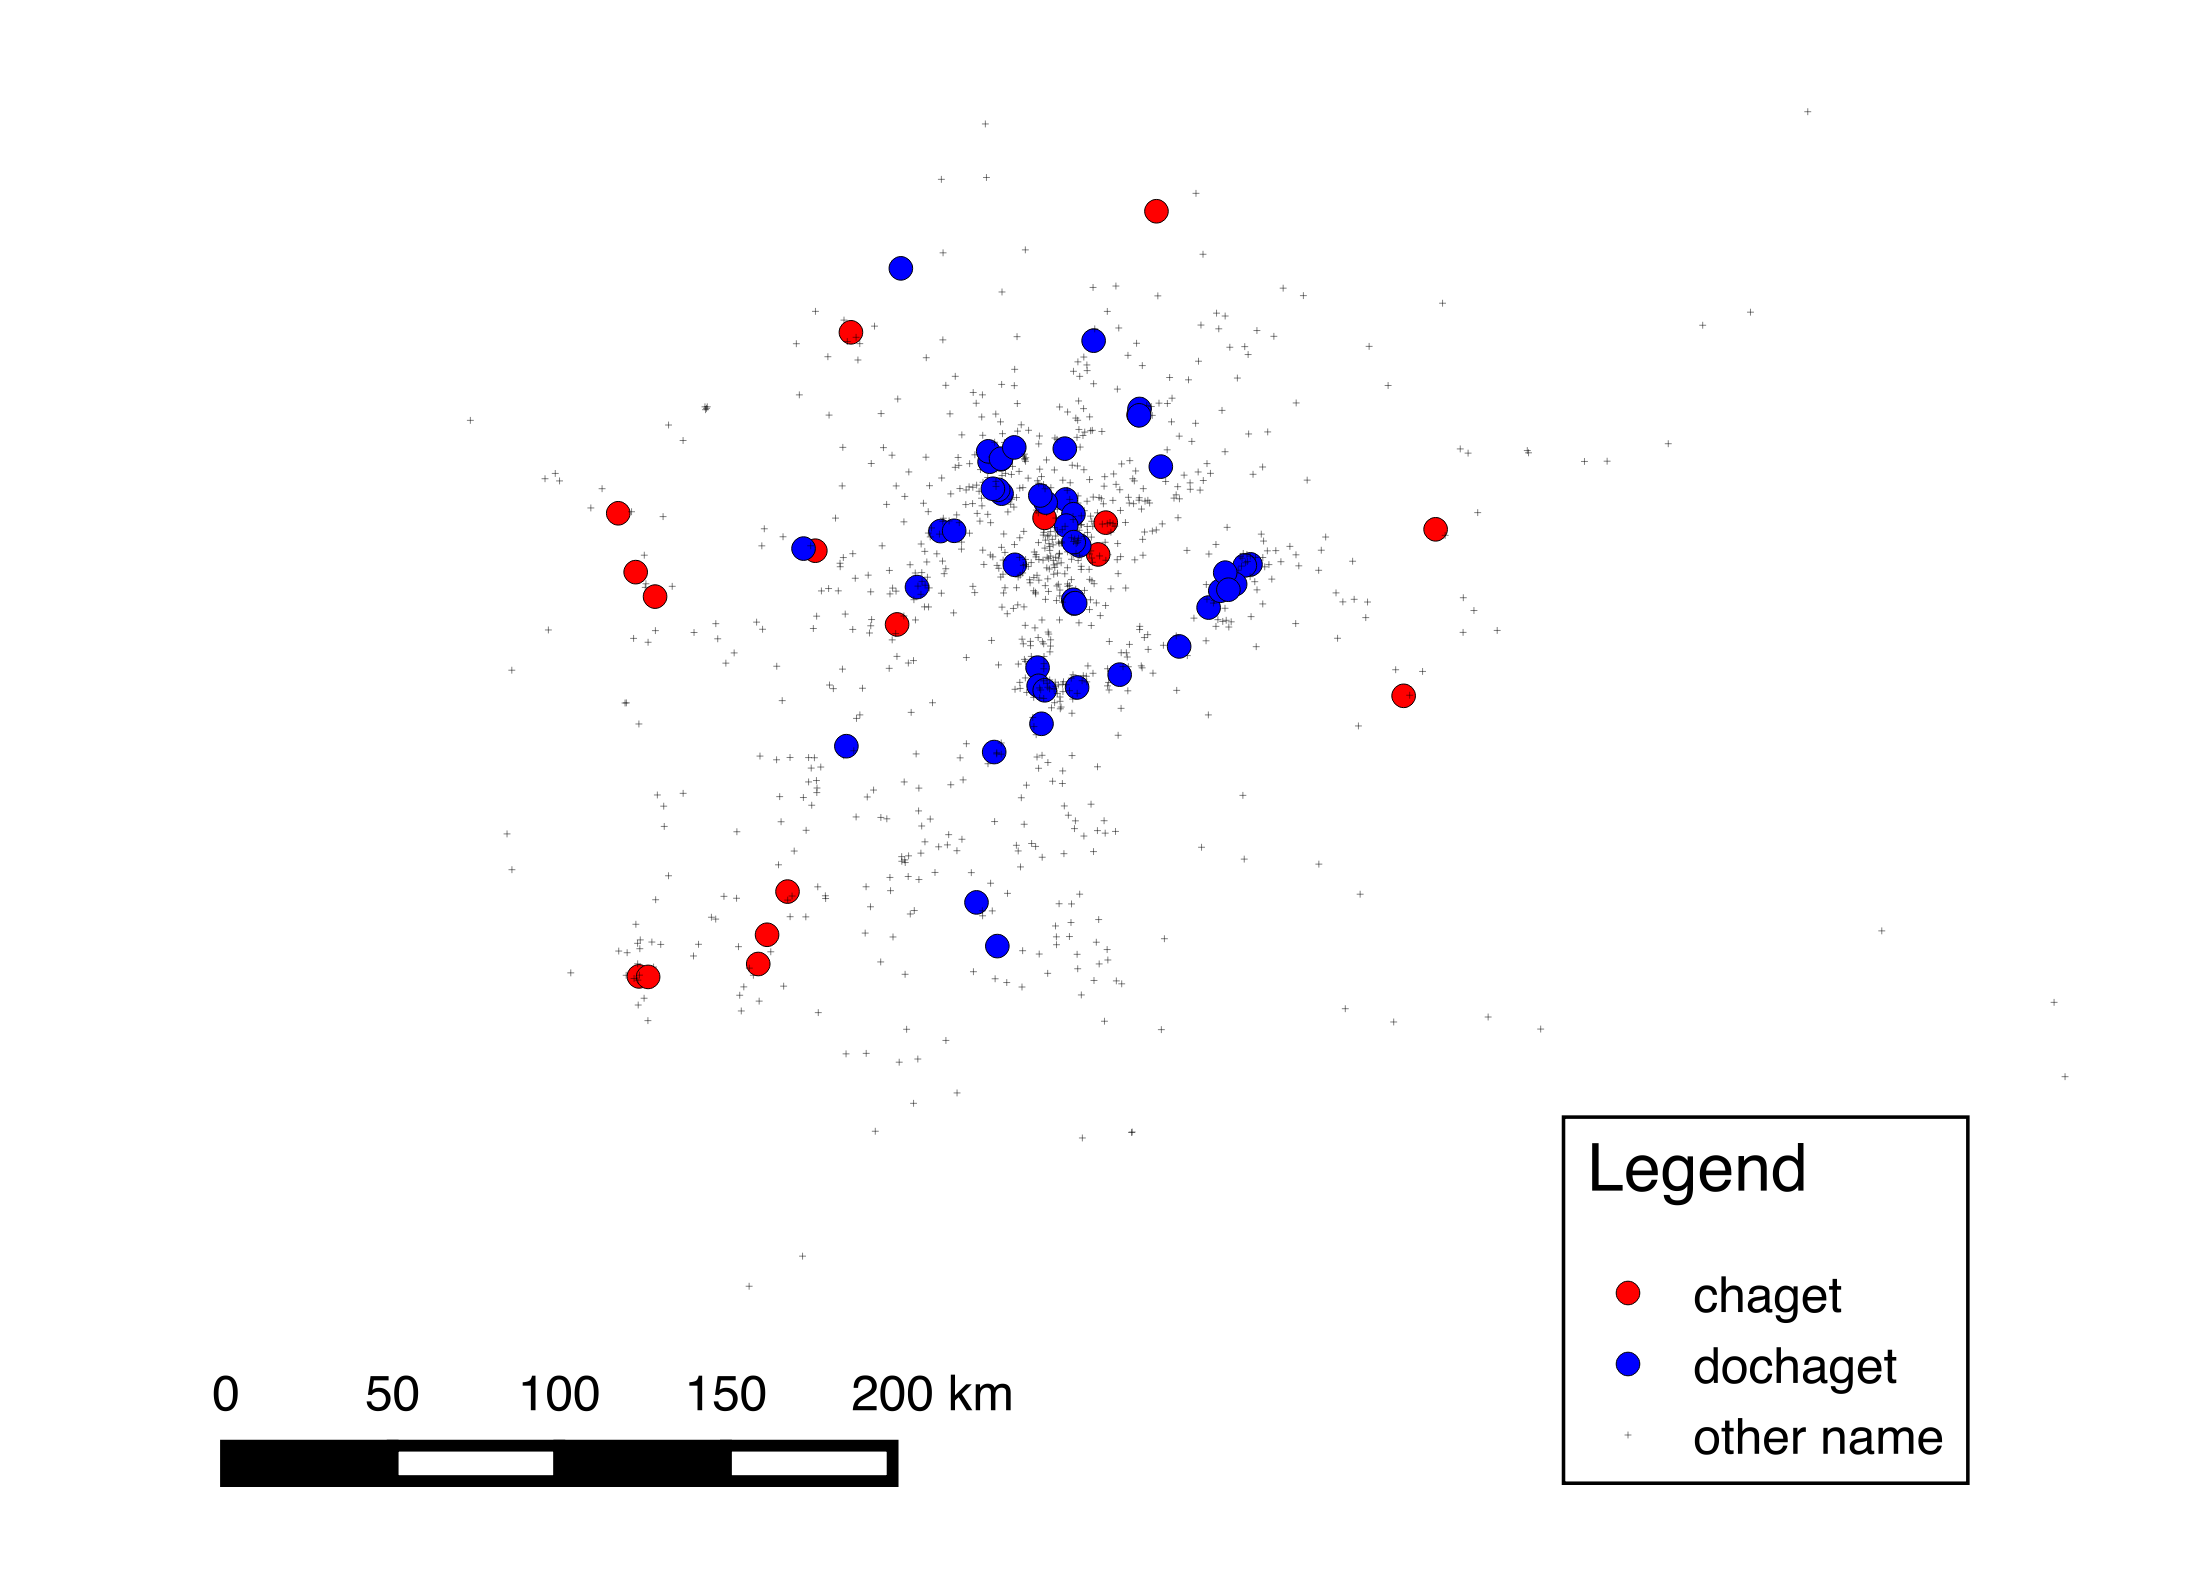
\includegraphics[width=0.9\textwidth]{figures/holton-fig1}
  \caption{Distribution of Lower Tanana names with generics \textit{chaget} and \textit{dochaget}}
  \label{holton:fig:1}
\end{figure}

There are even several instances of river mouth names which make use of a third form of the generic, \textit{khwdochaget}, a complex form including both the areal prefix \textit{khw-} and the \textit{do-} `orifice’ prefix. Consider the possibilities for a name based on the specific term \textit{Teyeddha’} and a generic ‘river mouth’. Since there are three different ways of expressing ‘river mouth’, there are at least three possibilities for this name. In fact there are even more possibilities, because the specific term can be either \textit{Teyeddha'}, which is the specific occurring in the name of the stream \textit{Teyeddha' No'}, or else the name of the stream itself can be used as the specific from which the river mouth name is derived. the choice between whether the ‘river mouth’ generic substitutes for \textit{no’}  or is added to it doubles the number of possible names to six, as shown in \ref{holton:ex:chaget}. However,  only the final name \textit{Teyeddha' No' Khwdochaget} is attested, including both the generic \textit{no’} ‘river’ from the stream name and the generic \textit{khwdochaget}.



\begin{exe}
\ex Possible generative names based on the specific term \textit{Teyeddha’ (No')} and  generic `river mouth’ terms\label{holton:ex:chaget} 
\begin{xlist}
\ex \textit{*Teyeddha’ Chaget}
\ex \textit{*Teyeddha’ Dochaget}
\ex \textit{*Teyeddha’ Khwdochaget}
\ex \textit{*Teyeddha’ No’ Chaget}
\ex[*]{ \textit{*Teyeddha’ No’ Dochaget}}

\ex \textit{Teyeddha’ No’ Khwdochaget}

\end{xlist}
\end{exe}

\noindent
So even if we could predict that the name of a place located at a river mouth should be named by combining the associated specific term with a form of the generic \textit{chaget}, we would have no way of predicting whether this generic should be added on in addition to existing generics or substituted for them, nor would we know which form of \textit{chaget} to use. In sum, we could not predict the name. And of course, we would have no way of knowing whether a particular river mouth actually had a name.

\subsection{Size of  generative clusters}
As noted above, examples of clusters of names sharing a single specific term have been cited widely in research on Alaska Dene place names.  This gives the impression of a place-naming strategy which assigns specific names to certain regions and then identifies places within this region according to the appropriate landscape generic. The Ahtna cluster based on the specific term \textit{yidateni} was noted above. A example from Lower Tanana is the cluster of 11 names based on the specific \textit{troth} ‘wild potato (\textit{Hedysarum alpinum})’, shown in Table~\ref{holton:tab:troth}. This is a well-known example, as one of the names in the cluster, \textit{Troth Yeddha’}, was recently adopted by the US Board of Geographic Names as an official place name.


\begin{table}[h]
\centering
\caption{Cluster of names based on the specific \textit{troth} 'Indian potato (\textit{Hedysarum alpinum})’}\label{holton:tab:troth}
\small
\begin{tabular}{l | l}
\textbf{Name} & \textbf{literal translation}\\\hline
\textit{Troth Yeddha'} &
Indian potato ridge\\
\textit{Troth Yeddha' No'} &
Indian potato ridge stream\\
\textit{Troth Yeddha' No' Dochaget} &
Indian potato ridge stream mouth\\
\textit{Troth Yeddha' No' Khwyighilenhde} &
where current flows into Indian potato ridge stream\\
\textit{Troth Bena'} &
Indian potato lake \\
\textit{Tr'ekhwghodegi Troth Yeddha Bena'} &
upper Indian potato lake\\
\textit{Tr'ekhwghotthidi Troth Yeddha' Bena'} &
lowland Indian potato lake\\
\textit{Tr'ekhwghotthidi Troth Yeddha' Bena' Edileni} &
flows into lowland Indian potato lake\\
\textit{Tr'ekhwghotthidi Troth Yeddha' Bena' No'} &
lowland Indian potato lake stream\\
\textit{Troth Ghotthit} &
toward the water from Indian potato\\
\textit{Troth K’eti} &
among the Indian potatoes\\
\end{tabular}
\end{table}

The cluster based on \textit{troth} in Table~\ref{holton:tab:troth} rather large, but as it turns out it is also highly exceptional. In fact, in our survey of the Lower Tanana place names data this is the largest cluster which occurs. In fact, while generativity is an important place naming strategy, as shown in Figure~\ref{holton:fig:2} the majority of Lower Tanana names---66\%---do not occur in generative clusters. Of those names which do occur in generative clusters, 54\% occur in clusters of just two names. This constitutes 69\% of the 234 generative place name clusters identified in Lower Tanana. Elaborate generative naming patterns with clusters of five or more names are extremely rare. So while the cluster based on \textit{troth} may provide a striking example of generative naming in Lower Tanana, it is far from typical.


\begin{figure}[h]
  \centering
  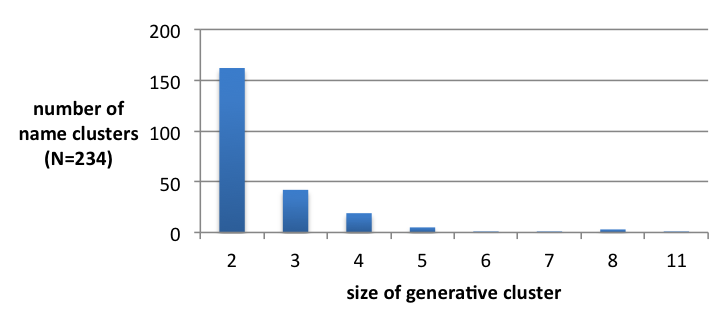
\includegraphics[width=0.9\textwidth]{figures/holton-fig2}
  \caption{Generativity of place names (number of clusters by size of cluster)}
  \label{holton:fig:2}
\end{figure}


Since the most common type of cluster is the cluster containing just two names, it is worth looking at these in more detail. Figure~\ref{holton:fig:3} breaks down the names occurring in clusters of two according to the generic term they occur with. The column labeled “none” refers to names containing no identifiable generic term. 21\% of the 324 names occurring in clusters of two. In addition, some 37\% of these names make use of the generic \textit{no’} ‘stream’; while another 24\% make use of the generic \textit{mena’} ‘lake’. Together names with these two generics and the names lacking a generic account for fully 92\% of the names occurring in clusters of size two.



\begin{figure}[h]
  \centering
  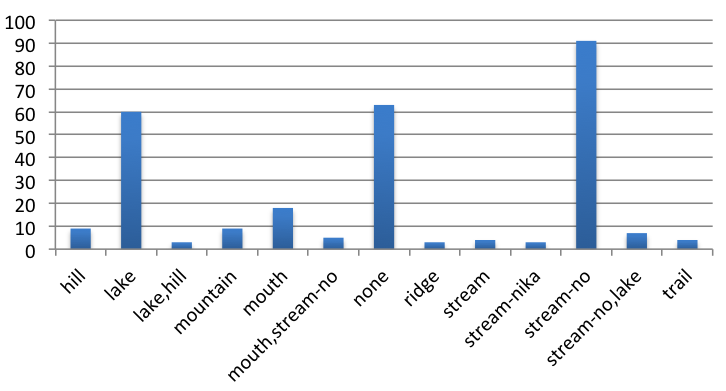
\includegraphics[width=0.9\textwidth]{figures/holton-fig3}
  \caption{Distribution of generative clusters of size=2 by type of generic}
  \label{holton:fig:3}
\end{figure}

What this means is that the primary use of the generative naming strategy is to name an associated stream or lake using the same specific term. Viewed in this context the Lower Tanana generative naming strategy seems a lot less exotic than would appear from the \textit{troth} example in Table~\ref{holton:tab:troth}. Indeed, the well-know language English frequently makes use of this strategy in naming rivers and lakes.

Generative clusters must by definition be geographically contiguous. It makes no sense to speak of two names which happen to share a specific term but are not other geographically related as being a cluster. However, there are many examples  of such non-clusters with shared specific term in Lower Tanana. The name \textit{Deba Ddhela’} and \textit{Deba No’}  share the generic \textit{deba} ‘sheep’ but are located more than 100 km from each other. Often additional qualifying material will be found in the specific term so that seeming clusters do not actually share the same generic. For example, there are two names based on the specific \textit{bezreya’} ‘land otter’, which do not cluster together. There are two additional names based on the specific \textit{bezreya’ toteth}  ‘land otter portage’; these names do cluster together, though not with the other two names based on \textit{bezreya’}. One could instead interpret \textit{toteth} ‘portage’ as a generic, in which case it might be possible to argue that names based on \textit{bezreya’ toteth}  and those based on just \textit{bezreya’} should be clustered together, but in this case the proposal fails on geographic criteria. Nevertheless, the issue of whether a particular component of a name should be treated as a specific or a generic remains. For this study we have limited ourselves to the standard set of generics outlined by \citet{kari2008}.

\subsection{Duplication of names}
\todo{not sure this section is necessary?}
It is often assumed that Dene languages avoid duplication of place names, and indeed, our study of Lower Tanana confirms that duplicate names are rare. However, the fact that names based on a single specific do not necessarily cluster together raises the possibility of name duplication, and indeed duplicate names do exist. Methodologically, the identification of duplicate names based on published sources is complicated in part by orthographic issues, as listed in Table~\ref{holton:tab:orthographic}.

\begin{table}[h]
	\centering%\small
\caption{Orthographic issues complicating the identification of duplicate names}\label{holton:tab:orthographic}
\begin{tabular}{l | l }
\textbf{Issue} & \textbf{Example} \\
\hline
vowel of possessive suffix can be represented as \textit{–e’} or \textit{–a’} & \makecell{\textit{Noghwya Bena’} \\ \textit{Noghwya Bene’} \vspace{5pt} }\\ 
%\hline
labial approximant may be represented as \textit{b}  or \textit{m} & \makecell{ \textit{Ts’oneye Bene’} \\ \textit{Ts’oneye Mene’}  \vspace{5pt}  } \\
%\hline
locative generic may be written \textit{de} or \textit{denh} & \makecell{ \textit{Nonudalyode} \\ \textit{Nonudalyodenh}\vspace{5pt} }\\
%\hline
word segmentation may vary & \makecell{ \textit{Teyh Yidatltoni} \\ \textit{Teyh Yi Datltoni} \vspace{5pt} } \\
%\hline
possessive morphology (glottal stop suffix) may be absent & \makecell{ \vspace{5pt}\textit{Khwdega’ Mena’} \\ \textit{Khwdega Mena’} \vspace{5pt}} \\

\end{tabular}
\end{table}

In order to assess to degree of name duplication in Lower Tanana we normalized the dataset to eliminate purely orthographic variation. Having done this we find that 88\% of the Lower Tanana names are unique, while another 8\% of the names occurs as doublets with exactly two duplicates (40 distinct names denoting 80 places). The remaining 4\% of names are duplicated more than twice (10 distinct names denoting 38 places). These 10 names with multiple duplicates are listed in Table~\ref{holton:tab:duplicates}.


\begin{table}[h]
\centering
\caption{Duplicated names showing number of tokens of each}\label{holton:tab:duplicates}
\begin{tabular}{l | l | c} 
\textbf{Name} &  \textbf{Literal translation} & \textbf{Tokens} \\\hline
\textit{Tobo Bena’} &
swan lake &
 6\\
\textit{Benh Dasr Bena’} &
lake shallows lake &
 4\\
\textit{Ch’etontswkh No’} &
brown water creek &
 4\\
\textit{Sanh Tena} &
summer trail &
 4\\
\textit{Sresr No’} &
black bear creek &
 4\\
\textit{Tonełkwn’ Bena’} &
clear water lake &
 4\\
\textit{Nogeddha Kan’} &
fox den &
 3\\
\textit{Teyh Chwkh} &
big hill &
 3\\
\textit{Tr’achenhnił’ode} &
where flat extends &
 3\\
\textit{Tr’iyh Tenet} &
canoe trail &
 3\\
\end{tabular}
\end{table}

Using data from the neighboring Tanacross language \citet{holton2009c} speculated that name duplication is in complementary distribution with generative names. That is, a given specific term may be repeated only if it is not used to form clusters. For example, the Tanacross name \textit{Ch’endaag Menn’}  ‘mineral lick lake’ is duplicated five times distributed roughly evenly across Tanacross territory. The name does not occur in any generative clusters. That is, there is no ‘mineral lick mountain’, ‘mineral lick stream’, etc. In fact, the specific term \textit{ch’endaag} does not occur in any other names. On the other hand, Tanacross names which occur in generative clusters appear not to be duplicated. For example, the Tanacross specific \textit{ch’inchedl}  ‘nose’ generates a cluster of four names located in close proximity, but there are no other Tanacross names which contain this specific term.

Whether or not this hypothesis regarding the complementary distribution of duplicated and generative names holds up for Tanacross, it is clearly not valid for Lower Tanana. In Lower Tanana a duplicate name may occur as part of more than one generative cluster. For example, there are two clusters consisting of \textit{Dets’eni Mena’} ‘duck lake’ and \textit{Dets’eni Mena’ No’} ‘duck lake creek’, so both of these names are duplicated and also part of generative clusters. Further, there is no constraint that Lower Tanana duplicated names be located far apart. The two instances of \textit{Noghwya Mena’} are some 64 km apart, while the two instances of \textit{Ch’elok’wy’ Teyh}  are only 4 km apart.

\section{Place naming strategies}

While the generative capacity in Lower Tanana place-naming is significant, it fails to account for a majority of Lower Tanana names. That is, the vast majority of Lower Tanana names do not occur in generative clusters. Moreover, the generative pattern does not reliably predict either the form of a name or the existence of a name for a particular place. To gain insight into place-naming strategies we must look beyond morphology and seek information about why and how particular places came to acquire their names. This requires examining the semantics of the names. For example, a name such as \textit{K'iyh Ddheł} `birch hill', which describes a  feature of the environment, can be semantically distinguished from a name such as \textit{Ch'etebił No'} `lynx snare creek', which refers to a use or function.  

Further insight into the semantics of place names can be gained  by asking speakers why places are named and by analyzing place-naming stories. In the case of Lower Tanana, this methodology is complicated by the fact that the language and its place names are remembered by only a few elderly speakers. However, we are fortunate to be able to draw on a large body of archival recordings, including many place name interviews collected in the 1970's as part of the Alaska Native Claims Settlement Act. In these recordings  the interviewers often ask directly about why a place has the name that it has. This information must of course be treated with caution, as such direct questioning invites folk etymologies. Fortunately, in the recordings that we have reviewed, the speakers are quite conservative in their responses, hesitant to offer speculative etymologies for name with which they are unfamiliar. In many cases speakers not only know why a place was named as it is but also who named it and when. This level of intimacy with places and names provides some assurance that the explanations offered by speakers on the recordings are not colored by folk etymology. 


Based on an empirical analysis of 20 legacy recordings of place name interviews we identify five primary place naming strategies used in Lower Tanana (Table~\ref{holton:tab:strategies}). These strategies are semantically defined, and thus it can sometimes be difficult to distinguish between then. For example, a place name which translates literally as `sheep mountain' might be considered environmental, describing a feature of the environment (i.e., sheep are there), or it could be considered functional (i.e., we go there to hunt sheep). In only a small number of cases can place naming strategies be identified based solely on an analysis of the name and its literal translation, and it can be misleading to make assumptions based solely on the literal translation. A case in point from our work is the name \textit{Sresr Chaget}  ‘black bear river mouth’. This might be interpreted as a (biological) environmental name based on the animal name \textit{sresr}. However, speaker Peter John clearly indicates that this is an incidental name given because someone saw bear tracks there: “Bear, they just see the bear tracks once and they call it that way” (ANL6026a, 0:59). There is no reliable method of determining the naming strategy without input from Native speakers. 

Drawing on  the archival recordings we were able to identify a place naming strategy for 856 of the 1063 names in the list. In the following subsections we describe each of the five major strategies in more detail.

\begin{table}[h]
\centering
\caption{Major Lower Tanana place-naming strategies}\label{holton:tab:strategies}
\begin{tabular}{l | l}
\textbf{Strategy} & \textbf{Description}\\\hline
Environmental & describing the geographic, environmental, or biological features of a place\\
Incidental & recalling something that happened or was seen at a place\\
Functional & describing how a place is used (human affordance)\\
Metaphorical & describing what a place resembles\\
Personal & incorporating a personal name\\
\end{tabular}\end{table}



\begin{figure}[hb]
  \centering
  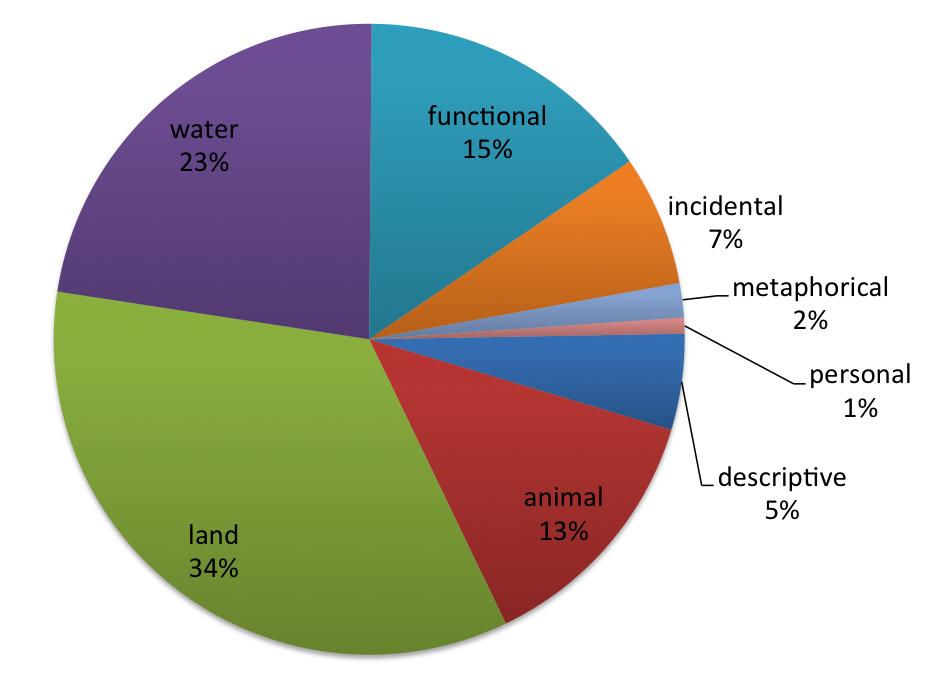
\includegraphics[width=0.6\textwidth]{figures/holton-fig4}
  \caption{Distribution of names by naming strategy \hl{Do we want to keep this pie chart?}}
  \label{holton:fig:4}
\end{figure}



\subsection{Environmental names}
We use the term \textsc{environmental} to classify place names that refer to geographic, environmental, or biological features. These features could be the size of a hill or field, the clarity of a body of water, how a river behaves in relation to the land, and what types of trees, fish, or other organisms than can be found at a location. This is a broad category within which we can identify three important subcategories: land, water, and animal. Environmental features referring to land and water dominate the Lower Tanana place naming system, accounting for more than half of the names for which a naming strategy has been identified (see Figure~\ref{holton:fig:4}). This emphasis on names which describe the environment is perhaps not unexpected given the close relationship between Lower Tanana people and their land- and waterscape. Indeed, the percentage of environmental names in Lower Tanana is comparable to that reported for Inuinnait by \citet[138]{collignon2006} and may be a significant feature of hunter-gatherer societies.

Several examples of names employing the environmental strategy are given in  Table~\ref{holton:tab:environmental}. The table lists the literal translation alongside the Lower Tanana name; however, the crucial criterion for determining that these are environmental names is verbal confirmation from speakers in the place name interviews. We avoided classifying names as environmental unless we could find evidence of speaker confirmation. One important caveat of this approach is that it does not account for potential tendency of a speaker to offer folk etymologies. Dene names are largely morphology transparent, so speakers have ready access to their literal meanings and could easily draw on this (consciously or not) in order to provide an environmental interpretation. Significantly, speakers do not consistently draw on the literal translation when providing an explanation for a name. As we shall see in the discussion of incidental names in the following section, in some cases speakers insist that the literal translation does not simply characterize the place but rather refers to a specific incident. As noted above, \textit{Sresr Chaget} ‘black bear river mouth’ is not a place with black bears but rather a place where a specific incident involving black bears occurred. In other words, speakers often know why places were named, and this topogenesis is a part of the knowledge of the name, obviating the need for a folk etymology.


\begin{table}[!h]
\caption{Names using the Environmental strategy}\label{holton:tab:environmental}
\begin{tabular}{L{3.5cm} | L{3cm} | L{3cm} | l} 
\small
{\bfseries Name} &
{\bfseries Literal Translation} &
{\bfseries Speaker Description} &
{\bfseries Recording}\\\hline

 \textit{K’iyh} \textit{Ttha} \textit{Nilani} &
‘the one with the young birch’ &
young birch &
0985b \\
 \textit{Tonełkwn’ Mena}’ &
‘clear water lake’ &
clear water; clear lake &
0987a; 0988a \\
 \textit{Chenh} \textit{Chwkh} &
‘big meadow’ &
big open flat with no trees on it &
0991a\\
\textit{Tu} \textit{Nadełdenh} &
‘where there is hot water’ &
hot water &
0989b \\
\textit{K’wy}’ \textit{Ch’eda}’ &
‘tough willow’ &
lake with willows on the side &
0989b; 6026b\\
 \textit{Nudh’onh} \textit{Mena}’ &
‘island is there lake’ &
island lake &
0984a\\
\textit{Beghentadhdleni} &
‘current flows behind  it’ &
the bend behind the hill &
0987b \\
\textit{The’odi} &
‘all the time’ &
you hear noise all the time, from the wind &
0984b

\\
\textit{Ch’enok’et} &
‘mineral lick’ &
moose lick salt there &
0985b \\
 \textit{Menh} \textit{K’wkhchwkh} &
‘on big lake’ &
big lake &
0988a \\
\textit{Dwkh} \textit{T’wkhde} &
‘elevated nest place’ &
nests in the tree &
0989a; 6018a\\
\textit{Khwtrela} &
‘moist place’ &
means wet &
0988a \\
\textit{T’egeth Yozra Nilani} &
‘cotton tree hill’ &
\textit{t’egheth yozra} means cotton tree; young cotton trees &
0984b; 6026a\\
\textit{K’wy’ Zrusr Yi Mena’} &
‘willow lake’ &
willow lake &
0984b\\
\textit{Thakwtadhlenh No’} &
‘ripple creek’ &
water running over rocks &
0984b \\
\textit{Ts’eba Nu’} &
‘spruce tree island’ &
speaker confirms spruce tree island &
0984b\\
\textit{K’iyh Tretr Ch’oghwna’} &
‘dry birch ridge’ &
birch on the ridge &
0987b\\
 \textit{Tr’ekhodetthatlde}  &
‘where it got chopped out’ &
they made a creek through there &
0987b\\
\textit{Łeyeth Toteth} &
‘dwarf birch portage’ &
little short willow &
0985b\\
\textit{Teyh Yitodaghi’odenh} &
‘slough extends into hill’ &
lake going in between the hill &
0987a\\
\end{tabular}
\end{table}

There is some danger of over-interpretation with environmental names. In particular, it is sometimes the case that environmental names don’t actually refer to existing geographic features. For example, the name \textit{Batr’a Ch’ilanh Teya’} means literally ‘obsidian is there hill’, but when questioned about the name, speaker Peter John is insistent that there is no obsidian on this hill. “No rocks there; they just named it like that. They only one that’s there is the little island.” (ANLC0989a, 00:26, 1975-05-25). The mere fact that a name describes an environmental feature does not necessarily imply that the name was given because of that description. Or it may be the case that speakers no longer have knowledge of the environmental features for which the place was named.

\subsection{Incidental names}
A small but significant portion of the Lower Tanana names refer not to the environment but to an event which occurred at the location named. We use the term \textsc{incidental} to denote a naming strategy that describes a event that occurred at a place or something that was observed at a place \citep[cf.][]{goehring1990}. Incidental names are not particularly frequent in the Lower Tanana corpus, comprising a mere 7\% of names, but they play a particularly important role in providing an historical connection to the landscape. The significance of incidental names cannot be directly inferred from the name itself or its literal translation. Rather, the name serves a sign which indexes an historical event. Knowledge of this event is an essential part of knowledge of the name. Of course, the names could be used and referred to without be aware of the associated event, but speakers repeatedly emphasize that knowledge of the associated event is a crucial part of knowing the name.

Some examples of incidental names are given in Table~\ref{holton:tab:incidental}. In some cases incidental names vividly describe the associated event, as with the name literally translated as ‘where a brown bear knocked someone down’. In other cases the associated event is more or less opaque, as with the name literally translated as ‘rabbit potlatch house’. These more opaque names “make sense” once you know the story of the event behind them, but there is no way to infer knowledge of the event from simply knowing the name itself.


\begin{table}[htb]
\caption{Names using the Incidental strategy}
\label{holton:tab:incidental}
\small
\begin{tabular}{l | L{3cm} | L{3cm} | l}
{\bfseries Name} &
{\bfseries Literal Translation} &
{\bfseries Speaker Description} &
{\bfseries Recording}\\\hline
\textit{Sresr Chaget} &
‘black bear mouth’ &
named so because they saw a set of bear tracks there once &
6018a\\
 \textit{Gwkh} \textit{Nitsił} &
‘rabbit potlatch house’ &
name comes from seeing one set of rabbit tracks &
6026b\\
\textit{Tsugi Tl’wgha’} &
‘marten’s grass’ &
caught a marten there &
0992a\\
 \textit{Dathdlazri Dena’iłghełdenh} &
‘where a brown bear knocked someone down’ &
a brown bear knocked us down &
0991b\\
\textit{Nu K’ech’idet’otthde} &
‘place where island is cut in two’ &
someone sliced island in two &
0985a\\
\textit{Tsoni} \textit{Tr’iłtanh} \textit{No}’ &
‘creek where we found a brown bear’ &
place where we saw a dead bear &
0991b\\
\textit{Dedenach’ilok} &
‘someone hurt us’ &
brown bear killed a man &
0987b\\
\textit{Dzak Todhyodenh} &
‘where Jack came’ &
First time they saw a white man at that place. His name was Jack. &
0987a\\
\textit{Ch’edhatr’eghikanh Nunkw} &
‘person got caught paddling doing something they’re not supposed to’ &
person got caught there and they killed him &
0988a \\
\end{tabular}
\end{table}

Speakers’ descriptions of incidental names may be quite vivid, reflecting the fact that such names are often embedded within a larger shared cultural memory. Regarding the name \textit{Dedenach’ilok} Peter John’s explanation is much more detailed than the literal translation ‘someone hurt us’ would indicate. John notes that a “brown bear killed a man right there” (ANLC0987b, 45:07). In some cases incidental names verge on the mythological, though speakers do not construe them as such. For example, in describing the name which translates literally as ‘place where island is cut in two’ Peter John says that {\textquotedbl}somebody got jealous and tried to fight with his wife, and he missed her with a knife{\textquotedbl} (ANLC0985a, 17:07). The implication here is that the physical separation in the island is a direct result of the knife cutting through the island after it missed its intended target.

It can sometimes be difficult to distinguish the incidental strategy from the environmental and functional strategies. The name \textit{Noghwya Ch’edonhden} means literally ‘where a frog had supper’. In our data speakers offered no further explanation for the name, so the strategy being used is unclear. If the place was home to many frogs, or even many flies for frogs to eat, it could be considered to be using the environmental strategy. However, it is equally possible that somebody once saw a frog eating there and named the place so, which would then be use of the incidental strategy. Without further consultation of a native speaker, the strategy will remain a mystery. Similarly, the name \textit{Gwkh} \textit{Nitsił} ‘rabbit potlatch house’ could be seen as a functional because the place functioned as a potlatch site. However, speakers insist that the place was named based on one instance of seeing rabbit tracks at this location, indicating that the incidental strategy is being used.

\subsection{Functional names}
We use the term \textsc{functional} to denote names which refer to how the places they denote are used. Functional names have a direct relevance to ecosystem services, since they describe the way humans relate to the land, or what \citet{levinson2008} calls human affordance. Places named for the use of animal snares or fish traps, graveyards or gravesites, and places that can be used to gather resources fall under this category. Functional names comprise 15\% of the Lower Tanana names. It could be argued that names for lakes and rivers that include the type of fish found there could be classified as ‘functional’, because one could speculate the lake would be used to catch that type of fish. But, for the purpose of this project, without the speaker expressly saying that is why the place was named, they will remain under the ‘descriptive’ category. Examples of the ‘functional’ strategy at work are shown in Table~\ref{holton:tab:functional}.


\begin{table}[htb]
\caption{Names using the Functional strategy}
\label{holton:tab:functional}
\small
\begin{tabular}{L{3.5cm} | L{3cm} | L{3cm} | l}
{\bfseries Name} &
{\bfseries Literal Translation} &
{\bfseries Speaker Description} &
{\bfseries Recording}\\\hline

 \textit{Ch’etebił} \textit{No’} &
‘lynx snare creek’ &
\textit{Ch’etebił} is an old name for a lynx snare &
6017a\\
\textit{Khwn’a Khwjeda’}  &
‘rotten river’ &
easy place to get lost &
0987a\\
 \textit{Niłk’ach’enidetl’unh} \textit{Mena}’ &
‘snares set on both sides lake’ &
means snares on both side &
0985b\\
 \textit{Bek’et} \textit{Notr’iyhtr’edełgoyi} &
‘on it we dry out a canoe’ &
we dry canoe on there &
0991b\\
 \textit{Nełtrith} \textit{Hał} \textit{Toteth} &
‘wolverine trap portage’ &
wolverine portage &
0985b\\
\textit{Ninotr’iyhleyahdenh} &
‘where canoes are left’ &
where they leave canoe to climb the hill &
0985b \\
 \textit{Bek’et} \textit{Tabił} \textit{K’at} \textit{Khwloyh} \textit{Mena}’ &
‘net places are on it lake’ &
where they used to set nets &
0987a\\
 \textit{Be’ot} \textit{Noyeghiłdhedenh} \textit{Tth’enhk’at} &
‘the grave of the one that was killed by his wife’ &
A woman killed her husband and that man was buried there &
0987b; 6026b\\
 \textit{Beghw} \textit{Tr’etreghi} &
‘by it we cry’ &
Lot of people used to go there and cry. Used to be village there with a big gravesite &
6030a\\
 \textit{Dwkhtso} \textit{Dedhlodenh} &
‘where there are caches’ &
cache is there, above the ground &
0989a\\
\textit{K’oł Tr’uneyh Ddhela’} &
‘we obtain whetstone mountain’ &
we pick stones for sharp knife or arrowhead (\textit{k’oł} `sharpening stone') &
0991b; 6026b; 6026a\\
\end{tabular}
\end{table}


Functional names share with incidental names an inherent human connection to the landscape, but whereas incidental names evoke a particular historical event, functional names refer to a continuing relationship with a place. In some cases the nature of this relationship is clear from the semantics of the name, but the meaning of other functional names is more opaque. For example, \textit{Khwn’a Khwjeda’} means literally ‘rotten river’, but in order to know why this river is considered rotten one must know more about the place and why it was named. Peter John explains that this place was named “because they got so many islands. There’s nothing but islands up there. They’re easy to get lost in.” (ANLC0987a, 45:09).

\subsection{Metaphorical names}
We use the term \textsc{metaphorical} to denote the naming strategy that uses metaphor to describe what a place resembles. This category is similar to what \citet[132]{collignon2006} calls morphological analogy. The metaphorical strategy is essentially a type of environmental naming strategy in that it makes reference to the appearance of a feature, but in using analogy metaphorical names reflect a greater degree of human interaction with the landscape. This is a rather small category; we identified only 15 names which use the metaphorical strategy, some of which are listed in the Table~\ref{holton:tab:metaphorical}.


\begin{table}[ht]
\caption{Names using the Metaphorical strategy}
\label{holton:tab:metaphorical}
\small
\begin{tabular}{L{3.5cm} | L{3cm} | L{3cm} | l}
{\bfseries Name} &
{\bfseries Literal Translation} &
{\bfseries Speaker Description} &
{\bfseries Recording}\\\hline

\textit{Tr’edhdo} &
‘someone is sitting’ &
rock formation looks like someone sitting down &
0987b\\
 \textit{Sresr} \textit{Yona}’ \textit{Tr’eghił’odenh} &
‘ram object extends out’ &
there are white rocks lined up that look like sheep walking &
6030a\\
 \textit{Seyatth’ena} \textit{No}’ &
‘my jawbone creek’ &
named for way it’s shaped &
0990a \\
\textit{Tr’iyh Khwt’ani} &
‘one like a canoe’ &
looks like a canoe &
0990a \\
\end{tabular}
\end{table}

Names in the Metaphorical category cannot be identified based solely on morphology and/or semantics but rely on speaker knowledge for their explication. For example, the name \textit{Tr’edhdo} means literally ‘someone is sitting’. This is the name of a long ridge north of Washington Creek (\textit{Tat’ali No’}), but the ridge is named for a particular rock formation which is located on the ridge—a rock formation which has the appearance of a seated figure (ANLC0987b, 40:45, 1979-05-24). On the other hand, some names which might at first appear metaphorical turn out to be descriptive once we consult speaker knowledge. For example, the name \textit{The’odi} translates literally as ‘all the time’, a rather ambiguous gloss for which it is tempting to provide a metaphorical interpretation. However, speakers are quite clear that this name is a reference to the observation that the wind blows all the time on this hill (ANLC0984a, 07:17). Hence, this name is not a metaphor but rather an environmental description.

\subsection{Commemorative names}
The \textsc{commemorative} naming strategy is used to classify those names which incorporate a personal name commemorating a particular person. We mention the commemorative strategy not because it is significant in Lower Tanana but rather because it is almost completely absent, found in only four names. Lower Tanana commemorative place names are not honorific, as are most English commemorative place names; rather, Lower Tanana commemorative place names refer to a place where someone does a certain activity. In this sense Lower Tanana commemorative names might be better characterized as personal names. The relationship is in some sense one of ownership, though this is ownership not in the sense of land tenure but rather in the sense of traditional use. The complete list of names using the commemorative strategy is given in Table~\ref{holton:tab:commemorative}.


\begin{table}
\caption{Names using the Commemorative strategy}
\label{holton:tab:commemorative}
\begin{tabular}{l | l | l | l} 
\small
{\bfseries Name} &
{\bfseries Literal Translation} &
{\bfseries Speaker Description} &
{\bfseries Recording}\\\hline

\textit{Sek’otl To’ Dazra’} &
‘Sek’otl To’s sandbar’ &
fish camp &
6030a\\
\textit{Doyelokh Beto’ Dazra’} &
‘Charlie Albert’s sandbar’ &
n/a &
none\\
\textit{Ywtltsetl’a Dazra’} &
‘Little Ywtl’s sandbar’ &
n/a &
none\\
 \textit{Bechots’idhił} &
‘Old Silas’ &
n/a &
none\\
\end{tabular}
\end{table}

All four of the names in Table~\ref{holton:tab:commemorative} make use of traditional Lower Tanana personal names, not modern English names which were later adopted by Dene speakers. This points to the names having an origin prior to the arrival of white settlers in the late nineteenth century. In two cases we know the corresponding English name as well. \textit{Doyelokh Beto’} is known in English as Charlie Albert, and \textit{Bechots’idhił} is known in English as Old Silas. Curiously, three of the four names include the generic \textit{dasr} ‘sandbar’ (possessed form \textit{dazra’}). We know from our corpus that at least one of these was a fish camp site; the remaining names are not discussed on the recordings. The one name without a generic, \textit{Bechots’idhił}, is said to refer to the location of a fox farm.

There is one additional place name in the corpus which incorporates a personal name: \textit{Dzak Todhyodenh} means literally ‘where Jack came’ and is known in English as Jack Hill. Speakers describe this as the place where they encountered the first White man, a man named Jack. So this name employs the Incidental strategy rather than the Commemorative strategy; it is not named after Jack but rather after the event of meeting Jack.

\section{Remaining challenges}

%\begin{itemize}
%\item Is generativity being under- or over-reported?
%\item How do we know what counts as a name if names are largely predictable?
%\item Just because we can predict what something would be named doesn’t mean it actually \textit{is} named.
%\item There \textit{is} variation in choice of generic, so less predictability than we might think.
%\end{itemize}

\subsection{What counts as a name?}

One of the greatest challenges for place names research is deciding just when something should count as a name. In some ways this problem is similar to the problem of deciding when a new term should be entered into a dictionary. Anyone can invent a way of a referring to something, but to be considered a place name such a reference should be conventionalized and broadly shared among a community of speakers. Moreover, a true place name should be stable over time. This criterion excludes ad-hoc forms of reference which are coined for particular speech event but then quickly discarded. Yet it is not always so easy to distinguish between ad-hoc and stable names. In English I might refer to the second of a series of three lakes as ‘second lake’, but when does this become a name rather than an ad-hoc reference. English provides some clues in the grammar, in that ad-hoc references to lakes are more likely to occur with an article, as in “Let’s go up to the second lake;” while names for lakes in English tend to occur without articles, as in “Let’s go up to Second Lake.” However, this criterion does not work with all English place names. We can easily speak of the Yukon River and the Lower Yukon River. The former is clearly a name, but the status of the latter is less clear. In any case not all languages offer such grammatical criteria for distinguishing names from ad-hoc references. In Dene languages if a stream is named \textit{Sresr No’} ‘black bear creek’, then the obvious way to refer to the lake which feeds the creek is \textit{Sresr Mena’} ‘black bear lake’ (or perhaps \textit{Sresr No' Mena'} `black bear stream lake'). Or it could just be unnamed. The fact that a name can be generated does not necessarily make it a name. The generative capacity in Dene naming is significant, but as we have seen it is not deterministic.

In particular, in spite of elaborate mechanisms for generating Dene place names, it is not the case that every form which can be generated will be a name. As noted above in the discussion of the use of the generic \textit{chaget} ‘river mouth’, naming is a deliberate practice, and speakers know what counts as a name. Thus, we must beware the tendency to over-differentiate and infer names for places which are actually unnamed. This caution is particularly relevant when working with severely endangered languages with few remaining speakers. Some existing reports may be problematic in this regard. For example, \citet{kari2012} list two lakes \textit{Khwgongw Nitl’et K’otena Mena’}  ‘upper cranberry lake’ and \textit{Khwghonhtthit Nitl’et K’otena Mena’} ‘lower cranberry lake’, distinguished by the directional terms \textit{khwgongw} ‘upland’ and \textit{khwghonhtthit} ‘lowland’. But when asked specifically about the names for these two lakes speaker Peter John was insistent that there was only one name. “The whole thing is what we call \textit{Nitl’et K’otena Mena’,} this whole thing, all this, all the lakes” (ANLC0985a, 27:37, 1979-05-24). Here we come up against differing conceptualization of the landscape. Lower Tanana assigns one name to a set of lakes, whereas as English insists on separate names for each lake. On this recording the English-speaking interviewers are clearly unhappy with Peter John’s response, since it doesn’t match their own conceptualization of the landscape.

Of course Lower Tanana speakers do have the directional terms ‘upland’ and ‘lowland’ available to them if they need to distinguish between the two lakes, but using directionals to distinguish places is not the same as naming them, any more than using upper and lower to distinguish parts of a river in English constitutes assigning a name to those parts of the river.
The key to understanding what places are named is that speakers know not only what is named but what is not named. Thus, speakers have knowledge of places which extends beyond simple inventories of names. Speakers often know what things are not named. For example, the string of islands in the Tanana River below the confluence with the Tolovana River is known as \textit{Nonudalyodenh}, literally ‘where islands extend across’. But speakers are keenly aware that only one of these islands, \textit{Khenge Nu’}, has a name; the others are known but unnamed places (ANLC0987a, 44:00).

\subsection{Optionality and variation of generic term}
In many cases speakers will freely omit the generic portion of a compound name when the referent is clear from the context, and it can be difficult to decide whether the generic is actually part of the name. This often occurs with the generic \textit{denh} ‘specific place’. Speakers will often omit the generic \textit{denh} when discussing a place. When questioned about the validity of the name \textit{Khwtethmenhdenh}, speakers explain that the name is actually \textit{Khwtethmenh} but that \textit{Khwtethmenhdenh} can be used when you’re talking to someone that doesn’t know where the place is (ANLC2556a, 2:34). Similarly, in an interview discussing the name \textit{Tr’enotokhwghiłch’ełdenh} is only pronounced with the generic \textit{denh} when introducing the name; five successive pronunciations of the name omit the generic and refer merely to that follow \textit{Tr’enotokhwghiłch’eł} (ANLC0989a). This suggests that for at least some names the generic \textit{denh} may not be a part of the place name. However, it is also possible that the name without the generic represents a clipping, similar to the way someone might use the form Everest for Mount Everest.

In some cases the historical recordings differ from the published place name list with respect to the presence of the generic. The name \textit{Dotron}’ \textit{Tr’iłtanhde} \textit{No}’ listed in Kari et al. (2012) contains two generics, \textit{de(nh)} and \textit{no’}, but in the recordings the name is consistently pronounced as \textit{Dotron}’ \textit{Tr’iłtanhde} \textit{No}’, without the generic \textit{de(nh)} (ANLC0984b)\textit{}. Similarly, the name listed as \textit{Tl’wkh Dhoydenh} in Kari et al. (2012) is consistently pronounced on the recordings without a generic as \textit{Tl’wkh Dhoy}, literally ‘grass sand’ (ANLC6026b).
There are also instances of names for which speakers vary as to the choice of generic. The name \textit{Nonudalyodenh} is also pronounced as \textit{Nonudalyokhw}, the latter form substituting the generic \textit{khw} ‘area’ for the generic \textit{denh} ‘specific place’ (ANLC0987a; ANLC0992a; ANLC6026b). It is not clear that there is any meaning difference, e.g., denoting a greater or lesser expanse. Moreover, this place can equally be referred to as \textit{Nonudalyo}, without either generic\textit{} (ANLC0992a).

An even more striking case of variation in generic term can be found in the name \textit{Mentoli No’}, literally ‘flows among lakes creek’. Peter John explains that “people used to call it two different ways, \textit{Mentoli Chaget} and \textit{Mentoli No’}” (ANLC0987a, 10:52). That is, either the generic \textit{chaget} ‘rivermouth’ or \textit{no’} ‘creek’ can be used with this name. When questioned regarding this Peter John insists that “\textit{chaget} means creek.”

\subsection{Names can change}
Names are not permanent but can change over time. In Lower Tanana the majority of the names are environmental and provide direct insight into the nature of the environment and the way humans experience the landscape. But as the environment changes the names can change too. Things that didn’t get used much didn’t get names. Places like lakes that have dried up and are no longer used, the names don’t get used. Speakers are often aware of places which used to be named but no longer have any names. Discussing a set of sloughs along the Tanana River, Peter John remarks, “Now over this way there used to be a lot of lakes over this way, and it’s all filled up with sand. And every one of them had a name, but then there’s no more lakes around there so they don’t use the name” (ANLC0988a, 26:45).

Speakers are also aware of places which used to have different names, though not all speakers necessarily remember the older names. Regarding the place known today as \textit{Dets’eni Trona’ Mena’} speaker Peter John says “That’s wrong name. It’s not \textit{Dets’eni Trona’ Mena’}. They just call it that. The young people right now today. But you go back one hundred years ago it’s \textit{Ts’u T’okh Mena’}…. That’s the old time way. \textit{Dets’eni Trona’ Mena’} that’s just the young people name that.” (ANLC0987a, 41:26). The newer name appears to be a calque of the unofficial English name Duckshit Lake. Some old names are still remembered centuries after they have ceased to be used. “\textit{Bedzeyh T’okh No’}, that’s the name of the Murphy Dome. Now, this is about 200 years ago. Now, after that, we call it \textit{Ts’etseye Bek’et Khenitighi’oyi}. After that, they say Murphy Dome.” (ANLC6026b, 18:45).

%names change (or disappear) because people stop using them (ANLC0988a, 26:34)
%Names can be transferred to another site. \hl{EXAMPLE}.

\section{Conclusion: Places get named for a reason}

Our study place of naming strategies in Lower Tanana reveals that the generative naming pattern is much less prominent than has been reported for other Alaska Dene languages. The vast majority of Lower Tanana place name clusters sharing a common specific term contain just two names. The often-cited clusters of multiple names generated by combining a single generic with multiple different generic terms are extremely rare. We have documented only six clusters of Lower Tanana names containing six of more names. In practice, Lower Tanana place naming is much less deterministic. A more economical explanation for the preponderance of the specific + generic naming pattern is the prevalence of the environmental naming strategy. More than half of Lower Tanana names describe environmental features referring to land or water. Given this tendency it is natural that many names incorporate landscape or waterscape generic terms.

The attractiveness of the generative hypothesis may be due to the analyzability of Dene place names. In his study of Ahtna places names, Kari notes that “...it is striking that 89\% of the names are fully analyzable” \citeyearpar[200]{kari2010}. However, this figure may actually be typical of morphologically complex languages. For example, \citet[103]{collignon2006} reports that fully 97\% of Inuinnait names are analyzable, and  \citet[78]{goehring1990} concludes that “in all cases save one the Inuktitut names are clearly translatable within the local context of the physical appearance or some aspect of human lived experience.” That is not to say that Dene and Inuktitut place-naming strategies are equivalent (in fact, they are quite different; see \citealt{holton2018b}); but the complex morphology exhibit in languages like Dene may lead us to view the generative strategy as more productive than it actually is. 




In the end, places get named not because a name can be generated but rather because of a conscious need to name a place. In other words, while a generative theory of place-naming in Lower Tanana can provide a post-hoc explanation for binomial names containing landscape generics, it has limited predictive value. For example, given the name for a certain creek we cannot predict that the name of a nearby lake will incorporate the same specific term. In fact, we cannot predict that the lake will even have a name. If the lake is named and does incorporate the same specific name as the creek, then we can posit a generative explanation. If not, then the generative theory fails. Indeed, we must consider the possibility that the so-called generative strategy may be epiphenomenal, existing only as a convenient post-hoc grouping of names which share a specific term.

What a generative theory of place naming fails to capture is that places get named for a reason. We have discussed some the Lower Tanana naming strategies above, but in each case the choice to deploy that strategy is deliberate. Place names provide a reference point for human interaction with the landscape. As Peter John remarks in the epigraph above, “People used to name these things as they see them” (ANLC0992a, 01:10). These attitudes toward place naming evidenced by Peter John and other speakers  in the Lower Tanana recordings are in fact similar to those reported for other Alaska Dene languages. Referring to Dena’ina names \citet[15]{evanoff2010} says “The place is named something special; you’ve been there, it’s named because it has to be passed on and it’s about something that was done there.... Everywhere you go it brings back memories of what happened there.” To quote Peter John once more, “The ones that they used more is the ones that got named.” (ANLC0988a, 26:34)


%As scholars from \citet{boas1934} to  \citet{basso1988} have repeatedly emphasized, names are not mere abstractions on the landscape. Rather, place names reflect speakers’ conceptualizations of the landscape and tell us something about how speakers relate to the land. That said, speakers do not have complete freedom when assigning names: place names are constrained by syntactic rules and by conventional patterns of naming. Speakers make use of language-specific place-naming strategies to create names. Most languages draw on multiple naming strategies. For example, English makes use of both a commemorative strategy (e.g., Mt. McKinley) and a resource-based strategy (e.g., Salmon Creek). Within Dene languages one strategy has received considerable attention in the literature.

As scholars from \citet{boas1934} to  \citet{basso1988} have repeatedly emphasized, names are not mere abstractions on the landscape. Rather, place names reflect speakers’ conceptualizations of the landscape and tell us something about how speakers relate to the land. Although this study of Lower Tanana place naming strategies is preliminary, our work shows the power of using archival recordings in order to understand Dene naming strategies. To date most work on Alaska Dene place names has focused on generating name inventories or on assembling travel narratives which cite place names as waypoints \citep[e.g.,][]{kari2010}. The groundbreaking work of \citet{kari1996a} to correlate the distribution of names with the morphological structure of those names reveals how a large place name database can support geographic analyses. By including archival recordings as well, we are able to examine not only morphology but also speaker knowledge of names---knowledge which is not necessarily recorded in the place name lists and cannot always be inferred from the morphology or semantics of the names. As access to place name inventories and archival recordings increases we can look forward to additional insights into Alaska Dene place-naming strategies and a better understanding of the complex relationship between Dene people and the land.

\refheading
\bibliographystyle{ldc}
\bibliography{holton}

\orcidfooter{Gary Holton}{holton@hawaii.edu}{0000-0002-9346-1572}
\orcidfooter{David Jason Harris}{djharris2@alaska.edu}{}

\label{holton-ch-end}


    \chapter[Tagish and Tlingit Place Naming Traditions of Southwestern Yukon]{\vspace{-25pt}Tagish and Tlingit Place Naming Traditions of Southwestern Yukon: Evidence of Language Shift}


\sethandle{10125/24845}

% Author last name as it appears in the header
\def\authorlast{Moore}

% change author in three references below to the actual author name so that this name is unique and matches the \label commands just below and at the end of the chapter
\renewcommand{\beginchapter}{\pageref{moore-ch-begin}}
\renewcommand{\finishchapter}{\pageref{moore-ch-end}}
\label{moore-ch-begin}



\thispagestyle{firststyle}

\chapauth{Patrick Moore}
\affiliation{University of British Columbia}

\authortoc{Patrick Moore}


\section{Introduction}
Indigenous place names from the southwestern Yukon reflect a historical shift from the widespread use of Tagish, a northern Dene (Athabaskan) language, to a predominance of Tlingit (a distantly related Na-Dene language). While language shift between indigenous languages has undoubtedly been a common process in many regions of North America, the southwestern Yukon is unusual in that the shift from Tagish to Tlingit occurred relatively recently. Research on indigenous place names has increased in recent years  because of anthropological interest in the cultural conceptualization of place and space, and because of the extensive documentation of land use related to indigenous land claims. Most of this work has focused on the place names of particular groups and regions, but some studies have also examined the contested nature of place naming in relation to colonialism, competing languages, language shift, and the displacement of indigenous peoples (Young 2001; Berg and Vuolteenaho 2009; Hercus, Hodges and Simpson 2009; Weinreich 2011). This study focuses specifically on the evidence that Tagish and Tlingit place names provide concerning the history of Tagish and Tlingit interaction and language shift in the southwest Yukon. This region is unusual in that a large number of place names have been recorded in both languages providing an opportunity to examine the processes of language change and evidence that Tagish was formerly the dominant language in this region but was gradually replaced by Tlingit.  While intermarriage between the coastal Tlingit and the adjacent Tagish of the Yukon interior was likely common even before the arrival of Europeans, Tlingits' control of the fur trade between the Pacific coast and the southern Yukon greatly increased their prestige and economic influence in the nineteenth century. Tagish adopted the Tlingit moiety and clan systems, and many adopted Tlingit personal names. According to Tagish speaker Daisy Smith (personal communication) by the late 1800s the remaining speakers of Tagish were all bilingual in Tlingit. The place names that form the basis of this study were originally recorded in both Tlingit and Tagish and identified on a map of the region by Angela Sidney and anthropologist Julie Cruikshank (Sidney 1980). Jeff Leer of the Alaska Native Language Center provided the Tlingit transcriptions of Sidney’s place names. For this article the transcriptions for the Tagish place names have been updated to a contemporary Tagish orthography developed by linguists working with the Yukon Native Language Centre\footnote{The symbols used in the Tagish alphabet are described on the Yukon Native Language Centre website at \url{http://www.ynlc.ca/tagish.shtml\#alphabet}}  and the translations and transcriptions of the Tlingit place names were rechecked with Bessie Cooley, a Tlingit speaker from Teslin, Yukon.\footnote{The Tlingit orthography used here is the same as the system developed by Gillian Story and Constance Naish and described on the Sealaska Heritage Foundation website at \url{http://www.sealaskaheritage.org/sites/defaults/files/tlingit_alphabet.swf}. The Naish/Story orthography is used in this article because it was the writing system used by Sydney and Cruikshank in their 1980 publication and because it remains in popular use. An alternative orthography for Tlingit was later developed by Jeff Leer and popularized by the Yukon Native Language Centre in their publications.}  The numbering of the examples is the same as in Sidney 1980, which is the source of all the place names in this chapter unless otherwise noted.

By the early twentieth century Tlingit was the predominant indigenous language in the Carcross and Tagish regions of southwestern Yukon, although a few families continued to speak Tagish as well as Tlingit and to use it with their children as well. The area also experienced an influx of English speakers after 1898 as it was situated on the main route to the Klondike Gold Rush. Tagish children who grew up in the early 1900s, among them Daisy Smith, Johnny Johns, and Angela Sidney, became some of the last fluent speakers of Tagish, and as adults worked with linguists and anthropologists to document their languages and cultures in the last decades of the twentieth century. Lucy Wren (personal communication), one of the last people to acquire first-language fluency in the language, recalled that her parents spoke to her only in Tlingit, but that Tagish was still commonly used between the adults in her home, and she was able to learn the language even though her parents avoided using it with her.	A small number of anthropologists and linguists documented Tagish language and culture the last half of the twentieth century. In the 1960s, anthropologist Catherine McClellan documented Tagish cultural practices, beliefs and stories (McClellan 1975, 2007). Later, linguists and anthropologists associated with the Yukon Native Languages Project, which became the Yukon Native Languages Centre, documented the Tagish language and Tagish traditions. Julie Cruikshank worked extensively with Mrs. Angela Sidney, a fluent speaker of both Tagish and Tlingit to document stories (Cruikshank 1989, 1992), genealogies (Sidney 1983), and place names (Sidney 1980). Victor Golla, Jeff Leer, John Ritter, and Patrick Moore worked with Tagish speakers, principally Angela Sidney and Lucy Wren, to record the language in the form of field notes, basic language lessons (Wren 2005-2007), and as audio and video recordings. Most of the Tagish language documentation is housed at the Yukon Native Language Centre, and a description of the Tagish alphabet, audio lessons, and audio storybooks are available from the Centre. A large number of Tagish recordings and written materials are also housed at the Alaska Native Language Archive of the Alaska Native Language Center and can be accessed online for non-commercial use.

\section{General Evidence of Length of Occupancy and Extent of Later Interaction}

The evidence from Tagish and Tlingit place names is consistent with the view that the area where Tlingit was spoken expanded, first northward within coastal Alaska and then into the interior.  Jeff Leer (1979) has argued for a northward expansion of Tlingit, since conservative features, such as constricted vowels, are found only in the southern Tongass dialect of Tlingit. In contrast, the Tagish language may have had a long history of development in the area where it was spoken in recent times. Based on a comparative study of terms for \textit{stream} in Dene (Athabaskan) languages, James Kari (1996a, 1996b) has argued that the historic Dene homeland was in the region where contemporary Dene languages use [tu·] for \textit{stream}, an area that includes the region where Tagish was historically spoken. This conservative word for \textit{stream} is evident in many of the place names that Cruikshank recorded with Angela Sidney (1980).\\

 Examples of Tagish place names with [tu·] for ‘stream’:
\begin{exe}

\exi{4.}	McClintock River
\sn Gēs Tū’è’ (Tagish)		king salmon river
\sn T’ahéeni (Tlingit) 		king salmon river
\exi{26.} 	Squanga Creek
\sn 	Dèsgwą̄gè Tū’è’ (Tagish)	Squanga whitefish creek
\sn 	Dasgwaanga Héeni (Tlingit)	Squanga whitefish creek
\end{exe}

Sidney learned Tlingit and Tagish as first languages and was able to provide terms in both for 68\% of the 130 locations. She identified 14\% of the places with only a Tagish name and nearly the same percentage, 18\%, with only Tlingit names. Some of the place names are composed of words from both languages, which indicates the extent of Tagish-Tlingit bilingualism, borrowing, and code-switching.\\

Examples of place names composed from both Tagish and Tlingit terms:
\begin{exe}
\exi{19.}	The single peak separated from Sinwaa, adjacent to the Tagish Road and the
turn-off from the Alaska Highway to Atlin, B.C.
	\sn Shgáa	T’ōh	 (Tlingit then Tagish)	Sidney says that shgáa is the Tlingit name of an
unidentified bird. Cooley was unfamiliar with the word.
The word is almost certainly Tlingit in any case since the sh-g syllable onset violates Tagish but not Tlingit phonological constraints.
T’ōh is Tagish for nest
\exi{55.} 	Tagish Hill
\sn Tā̀gish Tóoli	 (Tagish then Tlingit) Tā̀gish is the Tagish name for the Tagish narrows
	\sn		Tóoli is Tlingit for grassy hill
\exi{80.} Head of Tagish Narrows
\sn Tā̀gish Sháak	 (Tagish then Tlingit) Tā̀gish is the Tagish name for the Tagish narrows
\sn				Sháak is Tlingit for \textit{headwaters}
\end{exe}


The map in Figure~\ref{moore-map} indicates the location of the Tagish and Tlingit named places that are cited in this article. The reference numbers for these places on the map and in the article are the same as used in Sidney’s (1980) book and accompanying map.

\begin{figure}[h]
\centering
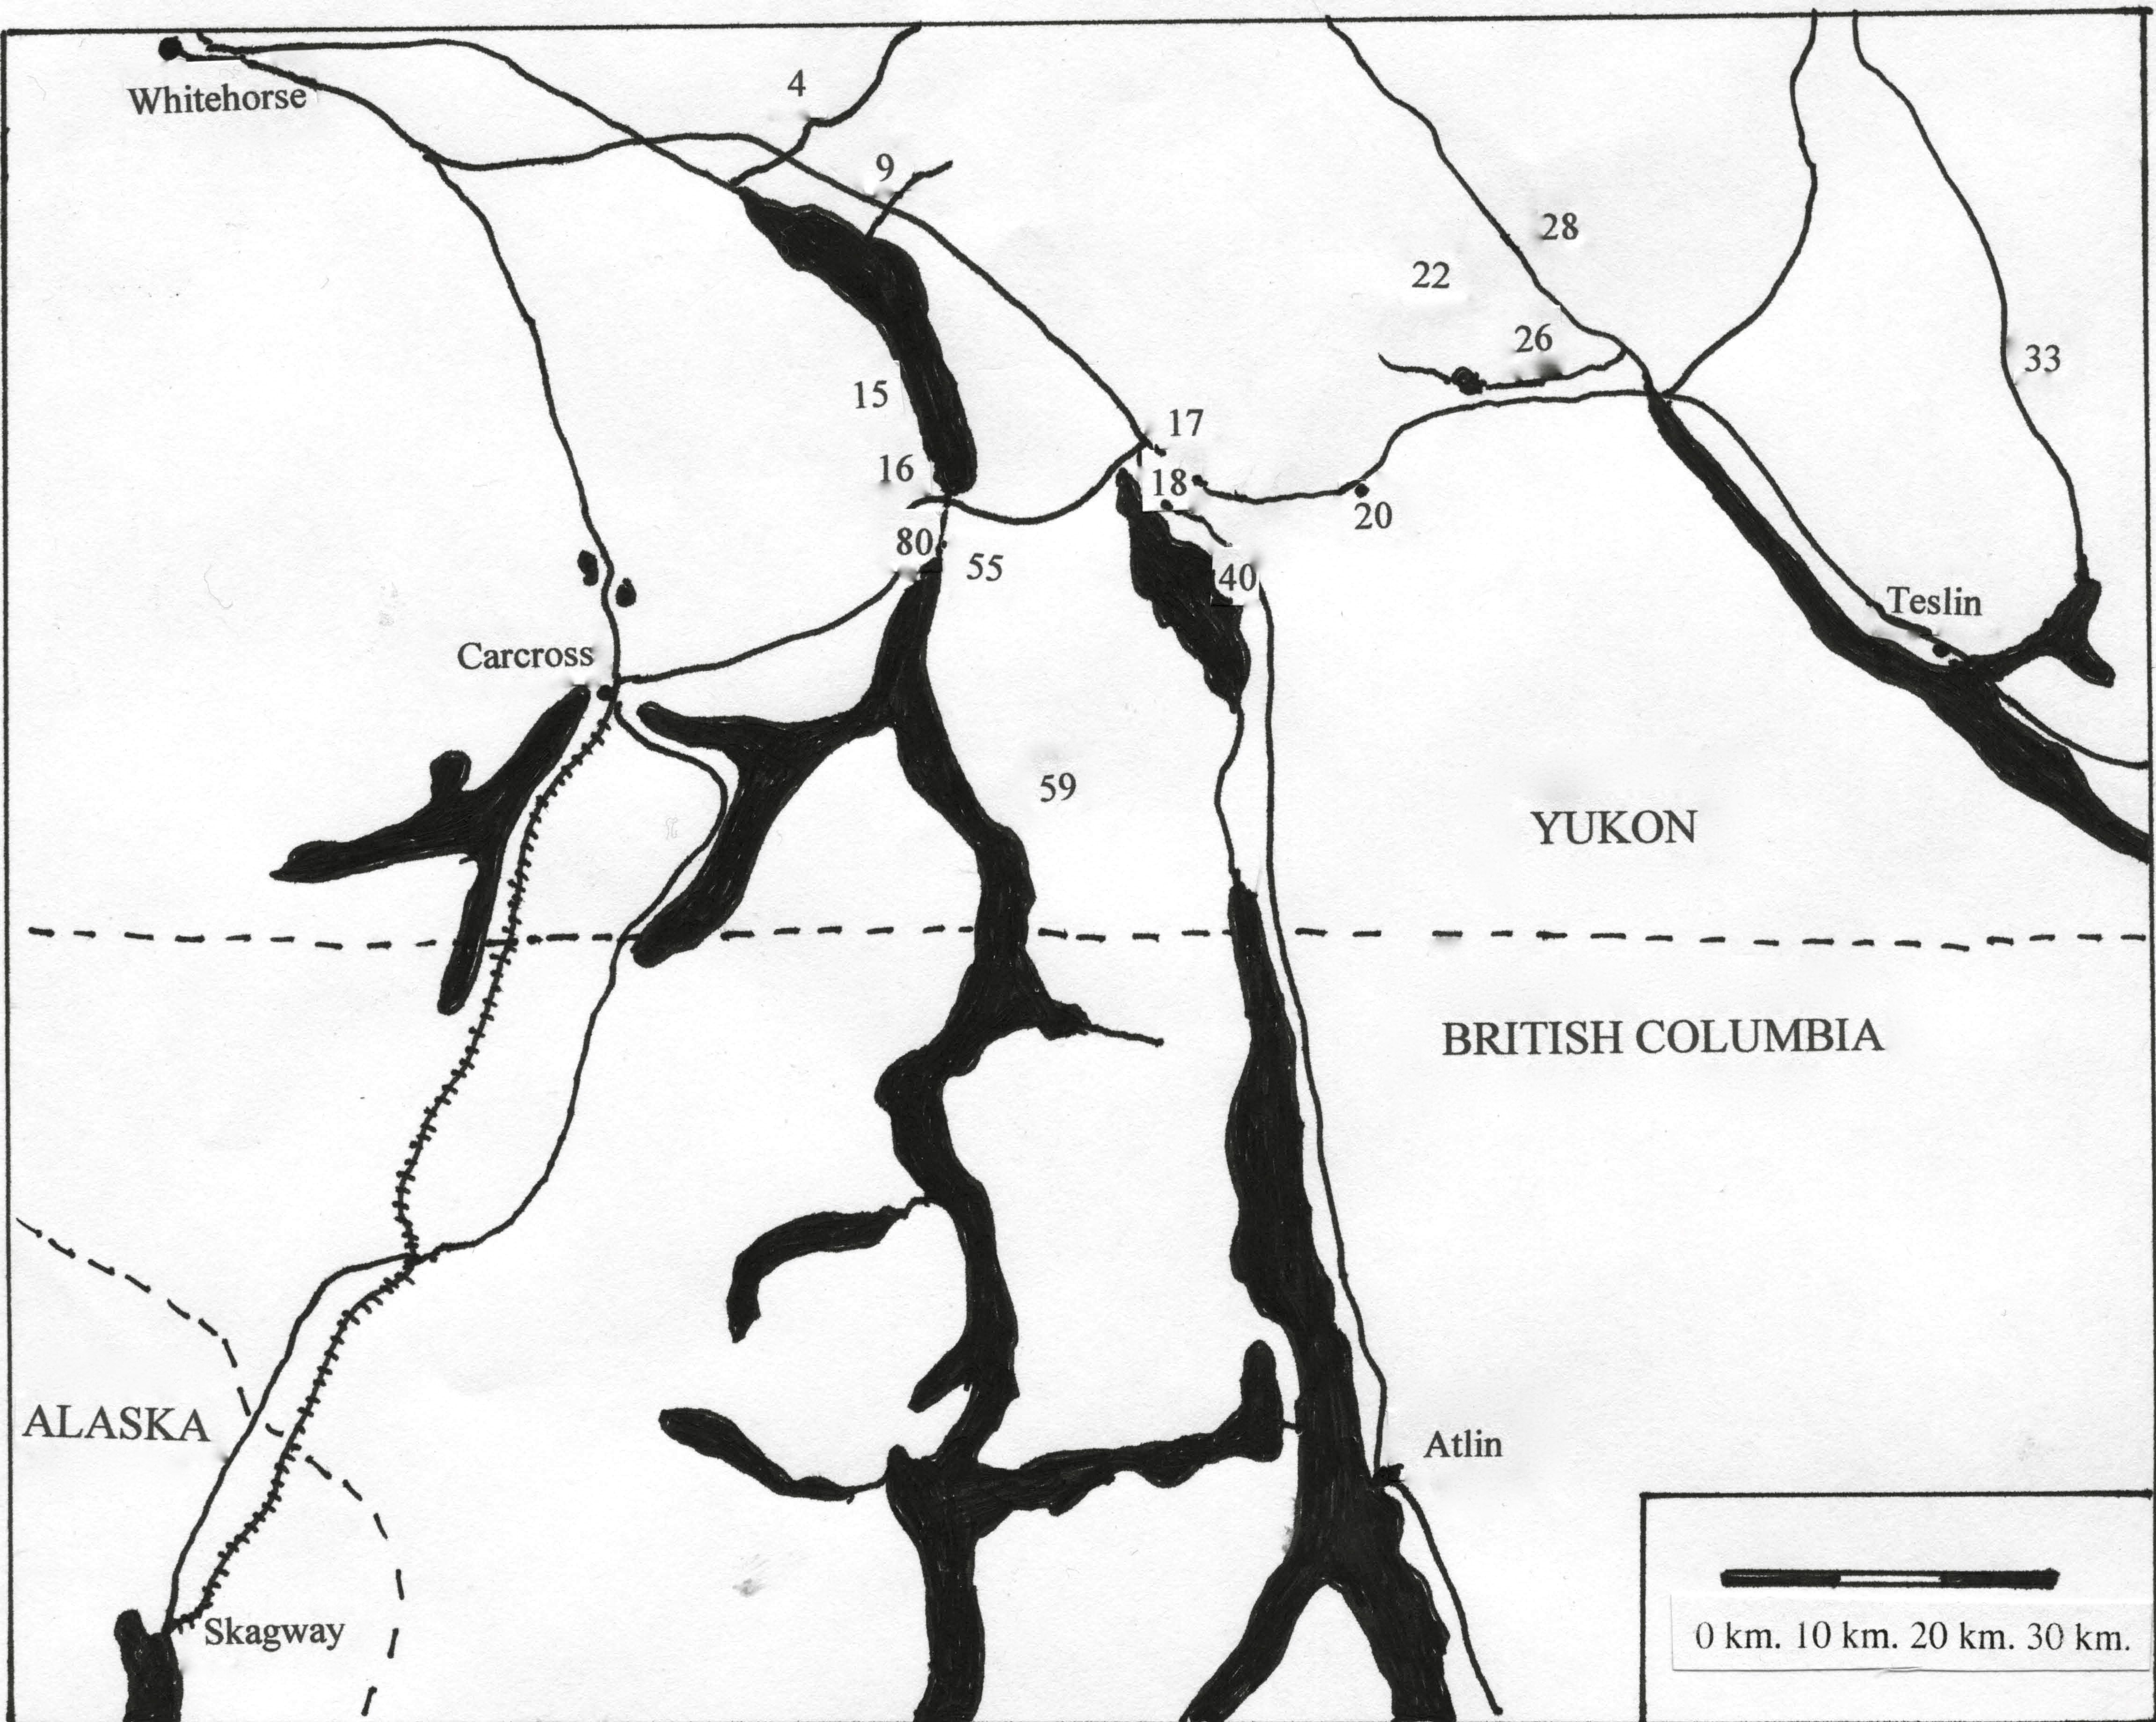
\includegraphics[width=0.9\textwidth]{figures/moore-fig1}
\caption{Locations of Selected Tagish and Tlingit Named Places}\label{moore-map}
\end{figure}

\section{Place Name Evidence of Language Shift from Tagish to Tlingit}
While all of the Tagish speakers were also fluent in Tlingit by the late 1800s, in the course of changing Tagish place names into Tlingit names they often modified the Tagish originals in ways that point to both Tagish as the source language and to the coastal connections of Tlingit. Some Tlingit place names (\textit{Sinwaa}, \textit{Nisaleen}) or parts of place names (\textit{Deisleen}) are not meaningful in Tlingit because they are based on the sound of the Tagish name. Some parts of Tagish names were omitted as they were translated into Tlingit, and in at least one case a Tlingit place name (\textit{Sheix’w X’aayi}) uses a term for a tree found in coastal southeast Alaska in a new sense in the interior.

While the Tlingit place names recorded by Angela Sidney are often composed of the same meaningful elements as the Tagish place name, in some cases, such as 18 below, the Tlingit term is based on the Tagish words modified to conform to the Tlingit sound system. In this case the Tlingit place name is not composed of elements that are meaningful in Tlingit.

Bessie Cooley (personal communication) says Sinwaa is also the name of a mountain near the Taku River (see also Nyman and Leer 1993 for confirmation of this term). It is possible that the Tlingit name for that mountain was also based on an Athabaskan name. Names referring to limestone, “grey rock,” may be common in Dene languages of this region. There is a Southern Tutchone name of the same form, \textit{Sima} (grey rock) which is the name of Golden Horn Mountain south of Whitehorse. The Tagish term from Lucy Wren is from the Tagish Literacy Workshop held in 1994 (Moore 1994: 15); the Tlingit term doesn’t mean limestone and is likely based on the sound of the Tagish word as it is only meaningful as a place name.\\

Tlingit place names based on the sound of the Tagish name:
\begin{exe}
\exi{18.} The mountain southeast of Jakes Corner between the Alaska Highway and the Atlin Road, excluding the first mountain peak.
	\sn Tsambā’a (Tagish, Angela Sidney)	`grey ridge'
	\sn Tsē Mbā (Tagish, Lucy Wren)		`grey rock'
	\sn Sinwaa (Tlingit from Athabaskan)
\exi{28.} Teslin River
	\sn Dèdèslīnī̀  (Tagish)			`water running off'
	\sn Deisleen Íxde Naadaayí		`Teslin running downstream'
\exi{33.} Nisutlin River
	\sn Dèslī́nī́ (Tagish)			(flowing [water?])
	\sn Nisaleen or Nilaseen (Tlingit)		(probably from Athabaskan)
\end{exe}



Tlingit speaker Bessie Cooley suggested ‘sneaks’ as a meaning for the Tlingit term Nisaleen, but it appears to be based on a Tagish word that includes the stem –līn, used in reference to flowing water, as in 28. The stem for “flowing water” may be commonly used in Dene (Athabaskan) place names since it also appears in other well-known names such as Deline (“where waters flow”) the North Slavey (and official English) name for the village at the headwaters of the Great Bear River on Great Bear Lake, Northwest Territories. The Tagish term in 33 is similar to the Tlingit (and English) terms for the village of Teslin, Yukon. The Tlingit (and English) terms for Nisutlin are likely based on a related Athabaskan word that had slightly different prefixes.
In other cases, such as 9 below, Sidney provided a Tlingit translation but indicated that the Tlingit place name wasn’t actually used to identify that location, and that everyone continued to use the Tagish term. The meaning of the Tlingit translation that Sydney provided for 9 below is unclear since Cooley was not familiar with the Tlingit term Keshuwaa (héeni means ‘stream’). Keshuwaa doesn’t mean ‘grayling’ which is t’áse or t’ási in interior Tlingit (likely from Athabaskan).\\

Tlingit translation not actually used as a place name designation:
\begin{exe}
	\exi{9.} 	Grayling Creek
	\sn T’àse Mbèt (Tagish)		`grayling food'
	\sn *Keshuwaa Héeni (Tlingit)	(*The Tlingit translation is not used.)
\end{exe}

At least one of the Tlingit terms that Sidney used in place names, the term for ‘red alder’ sheix’w in 15 below, has a different meaning than it would on the coast and reflects the extension of meanings in a new biotic zone. There are no red alder in the interior, the coastal Tlingit term is used by Tlingit in the interior as the nearest equivalent to red willow. Since the Tagish remained in the same biotic region, this sort of semantic shifts is not evident in Tagish place names.\\

Coastal Tlingit term given a new meaning in the Yukon interior:
\begin{exe}
\exi{15.} Point on the west Side of Marsh Lake
	\sn K’àye Desdel Nī (Tagish)	red willow point
\sn Sheix’w X’aayi (Tlingit)	red alder point
\end{exe}
\noindent
In other cases the Tagish name was simplified when it was translated into Tlingit by leaving out part of the Tagish place name.\\

Tagish place names that are simplified in Tlingit:
\begin{exe}
\exi{16.} A point on the west side of Marsh Lake, near Tagish Bridge
	\sn K’àlā Nī (Tagish)		`willow branches point'
	\sn K’ày’ lā Nī (Tagish)		`willow branches point'
	\sn Ch’áal’ X’aayi (Tlingit)		`willow point'
\exi{17.}  The mountain northeast of Jake’s corner, just north of the Alaska Highway
	\sn Tl’o K’ā̀’ Dzełè’	(Tagish)	`grass blade mountain
	\sn Chookanshaa (Tlingit)		`grass mountain
\exi{40.} Point of land on Little Atlin Lake, just north of the narrows
	\sn Mbesh Te’èts’et Nī (Tagish)	`where a knife fell into the water point
	\sn Lítaa Héent Uwaxixi (Tlingit)	`where a knife fell into the water
\exi{59.} Western extension of Jubilee Mountain
	\sn Kā̀’ Dḕtl’ōni Dzełè’ (Tagish)	`where arrows are tied in a bundle mountain'
	\sn Chooneit Shaayí  (Tlingit)	`arrow mountain' (translation from Athabaskan)
\end{exe}

The Tlingit place name Kaa  Léelk’u Shakanóox’u (below) may be a literal translation of the Tagish terms that loses the non-literal meaning of the Tagish original. In the case below the Tagish word for ling cod fish Kwachų̄ literally means “someone’s grandmother,” and when translated literally in Tlingit it loses the reference to the fish that live in the adjacent lake.\\

Place names that lose their non-literal meaning in translation to Tlingit:
\begin{exe}\exi{22.} “Streak Mountain”, north of Squanga Lake.
	\sn Kwachų̄ Tsī̀ts’enè’ (Tagish)	`ling cod skull'
(literally someone’s grandmother’s skull)
	\sn Kaa  Léelk’u Shakanóox’u (Tlingit)	`one’s grandmother’s skull'
\end{exe}

In both Tagish and Kaska, the names of specific fish or the generic word for fish may be used instead of the word for lake. According to Jeff Leer (personal communication) this place naming convention is not used in coastal Tlingit, so its use in interior Tlingit is evidence of the adoption of Tagish place naming practices as terms were translated into Tlingit. Bessie Cooley cited examples of interior Tlingit place names that use \textit{xáadi} (fish) to identify a lake, including \textit{Kaa Léelk’u Xáadi} (somebody’s grandparent [ling cod] fish), a lake near the south end of Teslin Lake, Yukon and X’aaa Xáadi (red fish), a lake near Teslin, Yukon. Examples from Kaska include \textit{Tets’egelūgé’} (up the hill fish), Watson Lake, 128° 47' W, 60° 08' N; \textit{Dzǭą̄lūgé’} (small bird fish), Little Bird Slough, 131°54' W, 62° 02' N; \textit{Bédelūgé’} (food fish),  a lake that is one of the sources of Blind Creek, 132°46' W, 62° 13' N, \textit{Eyānlūé’} (downstream people fish), No English name, 132° 01'W, 62° 08° N; \textit{Kūk’éhlūgé’} (next behind fish), No English name, 132° 31' W. 62° 31' W; Tāgeslūgé’ (middle fish), No English name, 132° 20' W, 62° 09' N; \textit{Tédāgīlūgé’} (up on top fish) No English name, 132° 44' W, 62° 04' N (Kaska Tribal Council 1997). Interestingly, most of the Kaska names that use \textit{lūge} or \textit{lūe} ‘fish’ as a designation for lakes (all the examples except \textit{Tets’egelūgé’}, which is in the Watson Lake area) are in the northern part of Kaska territory near Ross River, where there were formerly many speakers of Tagish.  In example 20 below the Tagish place name uses \textit{tā̀słeyī̀ }(pike fish) to designate the lake, while the Tlingit place name uses \textit{áayi} (lake).\\

Tagish place name using a fish name instead of ‘lake’:
\begin{exe}
\exi{20.} Squan Lake half way between Jake’s Corner and Squanga Lake. (Skwáan is a Tlingit personal name belonging to the Deisheetaan Clan. The lake may have been named for Joe Squan, or for someone else who held this name).
	\sn Skwān Tā̀słéyī 	(Tagish)	`Squan’s Pikefish'
	\sn Skwáan Áayi (Tlingit)		`Squan’s Lake'
\end{exe}



\section{Conclusion}
The Tagish and Tlingit place names recorded by Angela Sidney (1980) with Julie Cruikshank provide important evidence of both language shift from Tagish to Tlingit in this region of southwest Yukon, and an indication that most Tagish were fully bilingual in Tlingit. Most of the Tlingit place names Sidney recorded (68\%) are exact translations of the Tagish names (calques). There are also a number of place names that incorporate words from both languages, demonstrating that code switching and the use of loan words were common features associated with bilingualism. While most of the Tlingit place names are exact translations of the Tagish terms, the terms that differ provide evidence that the Tagish place names were in use prior to widespread language shift to Tlingit. The processes of simplification, basing Tlingit terms on the sound of Tagish terms, creating translated terms that lose their non-literal sense, adopting or failing to adopt different generic conventions (the use of “fish” for “lake”), and giving Tlingit terms a new semantic sense appropriate to their use in a new biotic zone are all processes that might be expected as a result of the expanded use of Tlingit. In addition to providing detailed information about traditional land and resource use, Sidney’s and Cruikshank’s documentation of the Tagish and Tlingit place names for 130 locations in southwestern Yukon also reveals much about the nature of Tagish and Tlingit bilingualism and local processes of language shift.




%%%% REFERENCES %%%%%%%%%%%%%%%
\refheading

\begin{hang}

Berg, Lawrence \& Jani Vuolteenaho. 2009.	\textit{Critical Toponymies: The Contested Politics of Place Naming}. Farnham, England, Burlington, Vermont: Ashgate.

Cruikshank, Julie. 1990. \textit{Life Lived Like a Story: Life Stories of Three Yukon Native Elders}. Vancouver: University of British Columbia Press.

Cruikshank, Julie. 1998. \textit{The Social Life of Stories: Narrative and Knowledge in the Yukon Territory}. Lincoln: University of Nebraska Press.

Hercus, Luise, Flavia Hodges \& Jane Simpson (eds.). 2009. \textit{Land is a Map: Placenames of Indigenous Origins in Australia}. Canberra: ANU Press.

Leer, Jeff. 1979. \textit{Proto-Athabaskan Verb Stem Variation Part One: Phonology}. Fairbanks: Alaska Native Language Centre, University of Alaska Fairbanks.

Kari, James. 1996a.	A Preliminary View of Hydronymic Districts in Northern Athabaskan Prehistory. \textit{Names} 44(4). 253-271.

Kari, James. 1996b. Names as Signs: The Distribution of ‘Stream’ and ‘Mountain’ in Alaska Athabaskan Languages. In Eloise Jelinek, Sally Midgette, Keren Rice \& Leslie Saxon (eds.), \textit{Athabaskan Language Studies: Essays in Honour of Robert Young}, 243-268. Albuquerque: University of New Mexico Press.

Kaska Tribal Council
1997	Guzāgi Kūgé’: Our Language Book: Nouns, Kaska, Mountain Slavey and Sekani. Whitehorse: Kaska Tribal Council.

McClellan, Catherine. 1975.	\textit{My Old People Say: An Ethnographic Survey of Southern Yukon Territory, Parts 1 and 2}. Ottawa National Museum of Man.

McClellan, Catherine. 2007.	\textit{My Old People’s Stories: A Legacy for Yukon First Nations}. Whitehorse: Yukon Tourism and Culture.

Moore, Patrick. 1994. \textit{Tagish Literacy Workshop}. Whitehorse, Yukon: Carcross Tagish First Nation.

Nyman, Elizabeth \& Jeff Leer. 1993 	\textit{Gágiwdułàt: Brought Forth to Reconfirm: the Legacy of a Taku River Tlingit Clan}. Whitehorse: Yukon Native Language Centre, Fairbanks: Alaska Native Language Center.

Sidney, Angela. 1980. \textit{Place Names of the Tagish Region, Southern Yukon}. Whitehorse: Council for Yukon Indians.

Sidney, Angela. 1983. \textit{Haa Shagóon: Our Family History}. Whitehorse, Yukon: Council for Yukon Indians.

Weinreich, Uriel. 2011. \textit{Languages in Contact: French, German and Romansch in Twentieth-Century Switzerland}. Amsterdam, Philadelphia: John Benjamins.

Wren, Lucy. n.d. \textit{Tagish Language Lessons}. Victoria British Columbia: FirstVoices, First Peoples Cultural Heritage Foundation. \url{http://www.firstvoices.com/explore/FV/sections/Data/Yukon/Tagish/Tagish}, accessed January 25, 2019.

Wren, Lucy. 2005-2007.	\textit{Tagish Language Lessons}. Whitehorse: Yukon Native Language Centre.
\url{http://www.ynlc.ca/tagish.shtml\#lessons}
accessed January 25, 2019.

Young, Kee How. 2001. The Politics and Aesthetics of Placenames in Sarawak. \textit{Anthropological Quarterly} 80(1). 65-91.

\end{hang}

\orcidfooter{Patrick Moore}{}{}

\label{moore-ch-end}


    \chapter[Direct borrowings and loan-translations of Navajo toponyms into New Mexican Spanish]{\vspace{-1.5in}
 {\normalfont\normalsize
\hspace{0.2\textwidth}\parbox{0.6\textwidth}{
\textit{``The human species...is composed of two distinct races, the men who borrow, and the men who lend.''}\\[2pt] \strut\hfill Charles Lamb, 1823\\\bigskip}}
\\ Direct borrowings and loan-translations of Navajo toponyms into New Mexican Spanish: Examples and explanations}


\sethandle{10125/24846}

\def\authorlast{Jett}
\renewcommand{\beginchapter}{\pageref{jett-ch-begin}}
\renewcommand{\finishchapter}{\pageref{jett-ch-end}}
\label{jett-ch-begin}



\thispagestyle{firststyle}

\chapauth{Stephen C. Jett}
\affiliation{University of California, Davis}
\authortoc{Stephen C. Jett}

\begin{Abstract}
Although Navajo culture reflects fusion with pre-existing Native cultures in the U.S. Southwest, the Navajo retained the language of the Athabaskan-speaking component that migrated southward from western Canada well over half a millennium ago.  Like other Athabaskan languages, Navajo resists linguistic borrowing and contains a minimum of placenames originating by either direct loan or loan-translation.  New Mexican Traditional Spanish, on the other hand, incorporated a fair number of toponyms from Navajo, occasionally by direct borrowing (of which seven probable examples are provided here) but much more often in the form of calques and quasi-calques (of which nearly three dozen likely instances are given).  This asymmetry reflects not only the intrinsic borrowing propensities of the two languages but also 1) the priority of Navajo in the region; 2) Hispanos’ making more, larger, and better-organized trading, slaving, and punitive intrusions into Navajo Country than did Navajos into Hispano territory; 3) post-1846 Anglo-Americans’ undertaking official exploratory and military expeditions into Navajo Country; and 4) Euroamericans’ use not only of Puebloan and Hispano guides and support personnel but also of guides and warriors from the functionally bilingual Cebolleta Navajo band, which cooperated against Navajos elsewhere.  Slaves who escaped or were released brought topographic and toponymic information back home as well, and were subsequently sometimes employed as guides. In addition, to an extent Navajo served as a regional lingua franca.
\end{Abstract}


%\vspace{1em}
\clearpage
\noindent
Placenames often lie on the land in metaphorical layers, and may “provide vital evidence for dating and, indeed, for estimating the mixture of races” over time (Gelling 1988:dust jacket).  They frequently reflect “the struggles for place that underlie the actual socio-cultural processes involved in naming[,] itself....  Recently there has been a recognition that place names ‘mark the spatiality of power relationships’ (Myers 1996: 237)” (Kearns \& Berg 2002: 284).  These things are well manifested in the American Southwest.

\section{The Navajo and the Navajo Language}

The Navajo (\textit{Dine’é} ‘People’) are a very populous American Indian nation of the southwestern United States, whose extensive reservations, allotted lands, and other occupied places (\textit{Diné Bikeyah} ‘Navajoland’)—which exceed West Virginia in total area—lie in the Four Corners Region of New Mexico, Arizona, and Utah (Kluckhohn \& Leighton 1946; Underhill 1956; Young 1961; Downs 1972; Iverson 2002).  The Navajo language is a Southern Athabaskan (Apachean) one, closely related to Northern Athabaskan (Dene) tongues of western Canada such as Chipewyan (\textit{Dënes\k{u}łiné}), Carrier (\textit{Dakelh),} Sarci (\textit{Tsuu T'ina}), and Beaver (\textit{Dane-zaa}), and less-closely akin to Alaskan Athabaskan idioms (Hoijer 1956; Dyen \& Aberle 1974; Young 1983).  Athabaskan is (with recently extinct Eyak) a branch of North America’s Na-Dené linguistic family; the latter appears to relate to western Siberia’s Yeniseian languages (Kari \& Potter 2010).

By at least A.D. 1400 and very possibly up to a century or more earlier, ancestral Athabaskan-speaking pre-Navajo hunter/fisher/gatherer peoples had moved southward along the Rocky Mountains from Canada, to the upper-middle San Juan River drainage of northern New Mexico (\textit{Dinétah} ‘Navajo Country’; Jett 1964; Seymour 2012; Matson \& Magne 2013; Haskell 1987; Perry 1991; Ives et al. 2014), merging to some extent with already-present non-Athabaskan farming indigenes (Brugge 2006) and adopting crop-raising, pottery-making (Brugge 1973), and Plains-Southwest fish-avoidance (Simoons 1994: 254).  The merger yielded a culture whose early form may today be echoed more in certain non-Navajo Apachean societies than among the \textit{Dine’é}.  Proto-Navajo culture was a hybrid, then, one which experienced subsequent cultural fusion with horticultural Puebloan culture, particularly from Tanoan-speaking Jémez but also from Zuni (whose language may be an isolate) and Uto-Aztecan- (UA-) speaking Hopi (on whose toponyms, see Ferguson et al. 1985 and Hedquist et al. 2014, respectively) and possibly Western Keres-speaking Ácoma and Laguna, occurring particularly during the latest seventeenth and early eighteenth centuries and yielding fully Navajo culture, which became increasingly dependent on farming and on livestock-raising based on Spanish-introduced sheep, goats, horses, and donkeys but which remained more mobile than that of Puebloans (Jett 1978).  This was accompanied by westward and southward territorial expansion (Hester 1962; Towner 1996) into Anasazi- (Ancestral Puebloan-) abandoned lands, a movement eventually accelerated by Ute raids after the latter had acquired firearms, which triggered evacuation of most of \textit{Dinétah}.  But despite the aforementioned fusion plus the absorption of a scattering of Utes, Southern Paiutes, Apaches, Hispanos, and so on, and despite a renowned general Navajo (and pan-Athabaskan) pragmatic tendency toward selective non-linguistic cultural incorporation (Farmer 1953; Vogt 1961: 327–328), the language (\textit{Diné Bizaad}) “has entirely preserved its original form” (Mirkowich 1941: 313).  As Jack Ives et al. (2014: 619) asserted, “Dene communities ... have a strong proclivity to protect language identities, yet they readily accept material culture and ceremonial life from neighboring societies.”

\section{Navajo, Spanish, and Toponymic Borrowing}

It is somewhat puzzling to read the following in the estimable \textit{The Spanish Language of New Mexico and Southern Colorado: A Linguistic Atlas}:

\begin{quote}
	Cobos (2003) \ldots identifies only two words as possibly from Navajo (\textit{chihuil} ‘small valley’ and \textit{josquere} in the phrase \textit{andar en el josquere} ‘to sow one’s wild oats’)....  However, the reverse direction of lexical influence was more substantial.  In Navajo, for example, the terms for ‘money (\textit{béeso} {\textless} \textit{peso}) and ‘Anglo’ (\textit{bilagáana}) were borrowed from Spanish \textit{peso} and \textit{Americano}, to mention only two everyday words.  (Bills \& Vigil 2008: 154)
\end{quote}

I have not identified plausible Navajo sources for either \textit{chihuil} (possibly, \textit{chíí’} ‘red’?) or \textit{josquere} (Studerus 2001: 73 deemed the former to be ``Of uncertain Indian origin”).  Neither am I, offhand, aware of Spanish non-toponymic lexical loans into Navajo other than the two that Bills and Vigil cite, plus \textit{siláo} {\textless} \textit{soldado} ‘soldier’, \textit{mandagíiya} {\textless} \textit{mantequilla} ‘butter’, \textit{bááh} \textless \textit{pan} `loaf bread', \textit{gowééh} \textless \textit{café} `coffee', \textit{bilasáana} {\textless} \textit{manzana} ‘apple’, \textit{tres} ‘three-spot playing-card’ {\textless} \textit{tres }‘three’, \textit{gíinse }‘fifteeen cents’ {\textless} \textit{quinze }‘fifteen’, and \textit{béégashi }‘cow’ {\textless} \textit{vaca}.  All these represent entities alien to the pre-Conquest \textit{Diné’é}.

These authors go on to observe that while Puebloan languages have absorbed numbers of words from Spanish, “it is most certainly the case that [New Mexican] Traditional Spanish has seen exceedingly little linguistic influence from the local Pueblo languages after four centuries of contact,” displaying a mere 16 such borrowings, several of which remain tentative.  They attribute this picture to there being several Puebloan tongues, to the existence of a proprietary Puebloan attitude respecting their languages, and to the Spaniards’ having been conquerors imbued with a sense of linguistic superiority.  The fact that the settlers’ were technologically more advanced and organizationally more elaborated presumably also played a notable role.

Adoption of pre-existing foreign placenames is one of the most common kinds of linguistic borrowing in contact situations, although, unsurprisingly, the degree of acquisition appears to be significantly conditioned by the hostile or pacific nature of the encounters involved (Callaghan \& Gamble 1996: 111–112) as well as by the level of intensity of the interactions.  Too, languages differ in terms of their degrees of intrinsic openness to the taking-in of foreign toponyms.  As has been mentioned, Athabaskan languages in general (including Navajo; Mirkowich 1941; La Farge 1975: 243; Jett 2001: 207; Kari 2011) are noted for their conservatism and their resistance to borrowing from other idioms (Sapir 1921: 209)---although the percentages of loan words vary dramatically among the many contemporary Athabaskan tongues (Brown 1994: 105).  This resistance applies to both general vocabulary and placenames but particularly to the latter (e.g., Kari 1989: 129).  Kari (2010) attributed this to both the complex Athabaskan verb morphology and speakers’ territorial ethos.

Toponymic conservatism may be especially strong in Navajo because adoption and adaptation of aspects of Puebloan mythology and ceremonialism have contributed to the Navajo perception that their topographic names were, for the most part, assigned by the supernaturals in mythic pre-\textit{Dine’é }times and are, therefore, divinely sanctioned and immutable (Jett 2014: 107; on Navajo religion, see Reichard 1990; on sacred places, see Watson 1964; Van Valkenburg 1974; Jett 1992; Kelley \& Francis 1994).

Nearly all Navajo toponyms are analyzable; typically, they are descriptive, sometimes possessive, and are neither corruptions of names borrowed from other languages nor currently-unsemantic archaic artifacts or otherwise-unetymological entities.  Some Puebloan-derived onamastic calques (names borrowed by translation) may exist in Navajo (most likely, of certain sacred places), but this is, so far, an entirely uninvestigated topic and my own limited observations suggest a dearth of such calques.  The sole example that has come to my attention is that of Ganado, AZ’s, Pueblo III- (P-III-) period Wide Reed Ruin, on Pueblo Colorado Wash, Navajo \textit{Lok’aah} (\textit{taa}) (\textit{Kin} [\textit{dah}])\textit{ Nteel} ‘Wide (Elevated) (House amidst) Reeds’, attested in 1902 (Ostermann 2004b:173; also, Franciscan Fathers 1910: 131) {\textless} Hopi \textit{Wukopakabi} ‘Wide Reed Place’, plausibly at the \textit{Ojo de Carrizo} ‘Reed Spring’ shown on Miera’s 1759 map (Kessell 2013: 36) and the \textit{Ojo del Carrizo} ‘Spring of the Reed’ mentioned in 1836 (Correll 1979: 159).

On the other hand, toponymic borrowing by translation from Navajo into Traditional Spanish has demonstrably occurred—if not massively, at least in multiple instances.  As the anthropologist for the Navajo Richard F. Van Valkenburg put it, “For some reason, with very few exceptions, Navaho names were shifted into Spanish use” (Van Valkenburg \& Walker 1945: 89; cf. Reichard 1990: 393), and he provided several examples (although his transcriptions and translations are in some cases a bit iffy); otherwise, the topic has never been systematically addressed.  The present paper aims to document, contextualize, and explain this phenomenon.

\section{New Mexican Spanish and Direct Toponymic Loans from Navajo}\label{jett:sec:3}

New Mexican Traditional Spanish evolved to dialect status during the centuries following the Colonial introduction of its ancestor, the then-current Mexican-Spanish “macro-dialect.”  Although it does not differ dramatically from other forms of New World Spanish, New Mexican does contain numbers of distinct lexemes, pronunciations, syntaxes, and usages and it preserves some archaisms.  In northern New Mexico/southern Colorado, it further differentiated into the Rio Arriba and Rio Abajo subdialects (Cobos 1983; Julyan 1998; Bills \& Vigil 2008; see below).

In contrast to large-scale acceptance of native placenames in much of colonized Ibero-America, the direct incorporation into New Mexican Spanish of Navajo names was uncommon—although the native names of a number of Indian \textit{pueblos} (e.g., Jémez, NM, and Ácoma, NM) and certain other locations carrying Puebloan designations (e.g., Abiquiú, NM) were retained.  Still, over a half dozen examples of borrowing from Navajo may be forwarded, most involving major geographic areas.

Black Creek Canyon, AZ, a gorge of moderate length cut into the Cutler Formation redbeds of the Defiance Plateau.  Van Valkenburgh (1945: 90) suggested that the Spanish names for this canyon---\textit{Cañón Chenelle} and \textit{Cañón de Calites}---were likely to be corruptions of the Navajo\textit{ Teeł Ch'ínít'i' Tsékooh} ‘Reeds-/Cattails-Extend-out-Horizontally-in-a-Narrow-Line Rock Canyon’.  This seems likely for the first of the Spanish names (attested 1864, Madsen 2010:map), but the \textit{Calites} of the second is probably a reflex of the Mexican (and New Mexican) Spanish Nahuatlism \textit{quelites} ‘edible greens, wild spinach (such as wild lamb’s-quarters, a chenopod)’ {\textless} Nahua (Aztec) \textit{quilitl} ‘edible greens’ (Santamaría 1959: 903; Cobos 1983: 141; Asociación de Academias de la Lengua Española 2010: 1799;  Julyan 1998: 281; Bye 1981; Bills \& Vigil 2008: 15; David M. Brugge, personal communication).  \textit{Teeł Ch'ínít'i'} ‘Reeds/Cattails-Extend-out-Horizontally-in-a-Narrow-Line ‘/\textit{Los Quelites} ‘The Edible Greens’ is nearby Oak Springs, AZ, currently a tiny dispersed Navajo settlement in a valley heading the canyon; this basin appears as Calites Cañon on von Egloffstein’s 1864 map (Madsen 2010: map). The name (as ``the Quelites,'' ``the Callitas Valley,'', ``the Calites,'' and ``Quilities'') appears in government reports dating to 1857, 1864, and 1866 (Correll 1979: 88, 168, 308, 327).

Canyon de Chelly, AZ, a long, branched, sheer-walled gorge in northeastern Arizona.  In the eighteenth and nineteenth centuries, this canyon system (along with Chinle Valley, or Valley of the Chelly, downstream of the canyon mouth) was probably the most agriculturally-productive and populous area within the Navajo Country as well as affording “fortresses,” defensible difficult-of-access cliff shelters and promontories used as hideouts and strongholds.  This area was, unsurprisingly, a major target of slavers and military expeditions from the capital, Santa Fé, and from the greater Rio Abajo country to the city’s south (see below).  The name \textit{Chelly} (also, as \textit{Chegui} and in multiple other spelling variants over the years) represents the Spanish attempt to pronounce and spell the Navajo name \textit{Tséyi’} ‘Within Rock, i.e., [Sheer-Walled] Rock Canyon’, a name attested as early as 1777 as well as in 1778, 1786, 1796, and repeatedly thereafter (Correll 1979: 82ff; Kessell 2013: 38; Reeve 1971a:105); cf. \textit{Arroyo}/\textit{Río de Chelly} ‘Chelly River’ (Chinle/Navajo Wash/Creek), \textit{Valle de Chelly} ‘Chelly Valley’ (Chinle Valley), and \textit{Sierra del Cañón de Chelly} ‘Range of the Chelly Canyon’ (the [Fort] Defiance Plateau, into which the canyon system is cut; also, \textit{Sierra María} ‘Mary Range’ or, perhaps, \textit{Sierra Amarilla} ‘Yellow Range’, after Fort Defiance, AZ, described below (Jett 2001: 43–45; Rice 1970: 72; Eidenbach 2012: 97).\footnote{On the 1778 Bernardo Miera y Pacheco map of the 1776 Atanasio Domínguez and Silvestre Vélez de Escalante expedition as well as on his related 1778 map, the Carrizo/Lukachukai chain is labeled \textit{Sierra de Chegui} ‘Mountain Range of Chelly’ (McNitt 1972:endpapers; Bailey 1964a:53; Van Valkenburgh 1999: 18; Kessell 2013: 38; Eidenbach 2012: 53), and the name was also used on the 1810 Humboldt map (based on 1804 work; Eidenbach 2012: 63).  A (non-existent) east-west range shown on the 1828 John Disturnell map is called \textit{Monte Chegui} ‘Chelly Mountain’ (Tyler 1985:frontis).  This designation appears later to have been transferred westward to the Defiance Plateau (which today’s local Navajos refer to as `the mountain').}

Chaco Canyon, NM, a broad, fairly-shallow, sandstone-walled east-west-trending canyon crossing the San Juan Basin:  \textit{Cañón de Chaco} ‘Chaco Canyon’ {\textless} Navajo \textit{Tsékooh}/\textit{Chékooh} ‘Rock Drainage or Canyon’ ({\textless} a generic); another suggested (but less-plausible) derivation of Chaco is {\textless} Navajo \textit{Tségai} ‘White Rock’ (Brugge 1986: 1).  An additional if unconvincing hypothesis is that the name derives from \textit{Tséyaa Chahałheeł Nlíní }‘The Darkness-Rock-Shelter Stream’ (Pearce 1965: 30; Linford 2005: 43).  The name \textit{Chaca} appears on Miera y Pacheco maps of 1778; Kessell 2013: 39; Van Valkenburgh 1999: 19; Briggs 1976) and on the 1828 Disturnell map (Tyler 1985:frontis).\footnote{Van Valkenburgh (1999: 19) proposed that Navajo \textit{tsékooh} was inspired by the Spanish designation \textit{Chaco} rather than the reverse, \textit{Chaco} being a name of mysterious derivation.  I think this unlikely.  Although the shift from \textit{é} (/eh/) in Navajo to (stressed) \textit{a} (/ah/) in Spanish is puzzling, there \textit{is} the (not-entirely-comparable) example in Spanish of \textit{San Diego}/\textit{Santiago}); note, also, \textit{ciénega}/\textit{ciénaga} and \textit{quelites}/\textit{calites}, discussed in the text.  Too, in New Mexican conjugated forms of the verb \textit{haber}, what is \textit{e} in Castillian may become \textit{a} (Bills \& Vigil 2008: 146).  There is an 1890 rendering, referring to the mid-nineteenth century, \textit{Río Chueco} (Conrad 1890: 228).  Perhaps the presence, in Colonial New Mexico, of the Spanish surname Chacón had an influence.  There is also the Spanish term \textit{charco} ‘puddle, pool’, which can refer to a \textit{tinaja} ‘jar’ (but, in the Southwest, also to a rock pool in the bed of an ephemeral stream) or to a stock tank (Cobos 1983: 224); the name \textit{Cañon del Charco} actually appears on an 1864 map (Eidenbach 2012: 120).  Note that although \textit{tsé} is the standard Navajo word for ‘rock’, it is modified to \textit{ché-} in \textit{chékoh}, in \textit{chézhin} ‘black [volcanic] rock’, and in several other compounds.  Note that the Spanish \textit{vaca} ‘cow’ entered Navajo as \textit{béégashii}.} The (redundant) \textit{Cañón de Chaco} is attested for 1819, 1821, the 1840s (Correll 1979: 120, 122, 170, 178, 185, 369, 401), 1858 (Brugge 1980: 14), and later; a \textit{Mesa de Chaco}/\textit{Chaca }‘Chaco Tableland’—presumably, adjacent Chacra Mesa (also known in Spanish as \textit{Mesa Azul} ‘Blue Tableland’)—was referred to in 1768, 1774, 1812, 1845 (Brugge 1980: 9–10, 13), and 1853 (Bailey 1964b:52; Brugge 1965: 17; Linford 2000: 183–184, 190–191), and a \textit{Río de Chaco} ‘Chaco River’, i.e., Chaco Wash, in 1864 (Madsen 2010:map).  \textit{Chacra} appears on a 1774 Miera map (Eidenbach 2012: 50, 53).  T. M. Pearce (1965: 30) asserted that that name was regional dialect for ‘desert’ (the word does not appear in Cobos 1983 or Bills \& Vigil 2008).  Note that Google Translate defines \textit{chacra} as ‘ranch’ and \textit{chaco} as ‘territory crossed by rivers and streams that form lakes and swamps’—not an apt description of normally-dry Chaco Canyon, whose floodplain seems not to have included significant swales.

“Chacolí,” NM.  Documented earlier than \textit{Chaco} (but not than \textit{Chaca}) is, to the southeast of Chaco Canyon, NM, and to the west of Jémez, NM, the \textit{Río de Chacoli} (or \textit{Chacalina} or \textit{Chaculín}) ‘Chacoli (or Chacalina) River’, in the formerly Navajo-occupied \textit{Valle de Chacoli} ‘Chacoli Valley’.  Díaz (2014: 61), writing of the 1779 Miera map, considered \textit{Chacolina} to be “possibly a reference to Chaco Wash,” perhaps thinking \textit{{}-ina} to be a diminuative suffix.  However, the places are in fact distinct.  This map of Miera’s displays the earliest appearance of \textit{Chacoli} that I have found, indicated to be a right-bank tributary of the \textit{Río Salado} ‘Salty River’, which flows into the \textit{Río Jémez} (Kessell 2013: 81; Eidenbach 2012: 54).  The \textit{Salado }does indeed have a right-bank tributary mapped today as \textit{Arroyo Cachulie }‘Cachuli Drainage’.  At the head of the \textit{Chacoli} is, according to Miera, the \textit{Ojo del Espititu Santo} ‘Spring of the Holy Spirit/Ghost’, conceivably today’s Soda Spring.  This is on the large historic Ojo del Espiritu Santo grant, established in 1815 (or possibly two decades earlier) and said to lie some six leagues from Jémez, NM (see Bowden 2004; USGS topographic map \textit{Holy Ghost Spring, NM}; if the Spanish geographical league of the era is meant, the distance would be about 24 miles).  It is conceivable that the topo map’s Cachulie is a misprint and that Chaculie was meant; this kind of error, though rare, does occasionally occur on such maps.  In Spanish, a \textit{cachuli} is a meal prepared to accompany a festive \textit{matanza} ‘livestock slaughtering/butchering (literally, killing)’ (El Bienhablao n.d.), which is a New Mexico tradition (The Santa Fe Site n.d.).  The arroyo could have been named for a \textit{matanza} meal that took place there long ago.  However, considering the apt location, it seems more likely that, instead, the name here represents modification of the original \textit{Chacolí} by metathesis, under the influence of the lexeme \textit{cachuli}.  Against this is the fact that today’s hot Holy Ghost Spring lies in the valley of Lopez Arroyo, a \textit{left}{}-bank tributary of the \textit{Salado} (Julyan 1998: 247).  This could be explained by positing that the latter spring takes its name from that of the land grant and is not the spring that originally lent its name to the grant.  In 1796, the toponym \textit{Chacoli }was listed with Chelly and Sevolleta (Cebolleta; see below), among other places (Correll 1979: 92; Reeve 1971a:105), suggesting that it possessed some importance.  In 1823, the explorer Antonio Vizcarra placed his \textit{El Chacoli} camp nine leagues (35.5 miles) from Jémez and two leagues (circa 8 miles) from the \textit{Río Puerco} (Linford 2005: 44)—which seems somewhat distant from both places but otherwise consistent (\textit{Río Puerco} ‘Dirty, Muddy [literally, Pig] River’ of the East; see Julyan 1998: 278; Bills \& Vigil 2008: 126; Navajo \textit{Naasisé }[\textit{Tééh}] ‘Enemy-Belt [Water Channel]’).  The designation\textit{ Chaculín }also appeared in\textit{ }1823 (Brugge 1980: 11).  In 1849, Lt. James H. Simpson stated that the \textit{Río de Chacoli} was “a small affluent of the Puerco.... a running stream four feet in breadth and a few inches in depth,” not part of the \textit{Río Jémez} watershed (McNitt 1964: 26, 28-29).  Richard H. Kern’s diary refers to this area as the “Chacalina valley.”  His map of the expedition shows the route crossing the \textit{Valle de Chacoli}, which runs southwestward to the \textit{Puerco} and which could be interpreted as the \textit{Rito Olguín} ‘Olguín Little River’ (Olguín is a surname).  However, the map shows the (unlabeled) \textit{Río Salado} also joining the \textit{Puerco} nearby (Fort Huachuca, Arizona n.d.), which is contrary to reality.  In light of all this confusion and considering Simpson’s description of his route (pp.\ 25-28), my surmise is that what Simpson thought to be a Puerco tributary and the \textit{Chacolí} was, in reality, the \textit{Salado} and that the party crossed the latter and then ascended the Cachulie (“a very shallow valley”; p.\ 28) and traversed the low  divide into the Puerco Valley.  \textit{Chacolí} and \textit{Chaculín}/\textit{Chacalín}[\textit{a}] would seem certainly to be Spanish versions of the (here, undocumented) Navajo \textit{Chékoohl\'{\k{i}}}[\textit{ní}]\textit{ }‘[The] Rock-Drainage Flow’.\footnote{The fact that a red wine of Viscayan Spain is called \textit{chacolí} (Williams 1955: 2:168) is doubtless fortuitous.  The word there is Basque, \textit{txakolin}, with \textit{txacolina} meaning ‘the chacolí’ (Wikipedia, “Txacoli”).  Similar, Kichwa-derived terms in South American Spanish also seem irrelevant.} A difficulty is that the Cachulie watershed is not rocky.  The \textit{Rito Olguín} does qualify as a rock drainage, but otherwise seems unlikely. Possibly relevant is a left-bank \textit{Salado }tributary downstream of the \textit{Arroyo Cachulie }called \textit{Arroyo Peñasco} ‘Boulder Waterflow’.  I speculate that the whole \textit{Salado} drainage—much of which is cliff-girt—constituted \textit{Chacolí} and that these tributary names are onamastic survivals in different forms.  Today’s Holy Ghost Spring\textit{ }could then be the same as Miera’s of 1779.  Although there exists the Mexican Nahuatlism \textit{chacalín} ‘freshwater prawn’ {\textless} Nahua \textit{chaculin} ‘\textit{Macrobrachium}’ (Asociación de Academias de la Lengua Española 2010: 464), in the U.S. Southwest neither that genus nor crayfish occurs to the west of the Great Plains (Bowles, Aziz \& Knight 2000; Wikipedia “Crayfish”).


Chuska Mountains, AZ/NM, a long, elevated plateau, which separates the Arizona and the New Mexico sections of the Navajo Country.  Also included with the aforementioned places in a 1796 list (as well as, frequently, in later years) are (\textit{Sierras de}) \textit{Chusca}, \textit{Tunicha}, and \textit{Carrizo}.  These (from south to north) are the three divisions of the forested north-south-trending Chuska (formerly, Tunicha) Mountains.  The first two names derive, respectively, from Navajo \textit{Ch'óshgai} ‘White Spruce’ (for Chuska Peak; Van Valkenburgh 1974: 171; Spanish version attested for 1776 and 1778; Julyan 1998: 83; Kessell 2013: 38; Eidenbach 2012: 53; also seen as Choiskai Plateau; Dutton 1886: 130) and from \textit{Tó Ntsaa} ‘Big Water/Spring’ (cf. Spanish \textit{Río Tunicha} ‘Tunicha River’, Chaco Wash); \textit{Carrizo} is a calque, discussed below (Correll 1979: 93, 114, 122, 143, 146, 147, 174; see also, Barnes \& Granger 1960: 8).

Penistaja, NM, a Hispano ghost village some ten miles to the west of Cuba, NM, in the \textit{Río Puerco} of the East drainage (see “Chacolí,” above; also, below).  According to Julyan (1998: 263), while the name Penistaja “has been said to be derived from the Spanish \textit{peña}, ‘boulder,’ more likely it’s a corruption of the Navajo name of the place, transliterated as \textit{binishdaahi” }(\textit{Bíniishdáhí }‘The One I Sit Down Against’).  On the other hand, Young and Morgan (1980: 243; followed by Kelley \& Francis 2018: 292) asserted that “The Navajo name mimics the Spanish.”  Thus, in this instance the direction of borrowing is ambiguous.


\section{Examples of Navajo Toponymic Calques in Southwestern Spanish}\label{jett:sec:4}

Spanish placenaming in Colonial New Mexico heavily stressed Roman Catholic Christian saints’ names; names of biblical concepts, miracles, and places; and the like.  However, in the North American Southwest many Spanish descriptive toponyms were coined, as well (e.g., \textit{Agua Azul} ‘Blue Water’, NM), plus a few metaphorical ones (e.g., NM’s \textit{La Alesna} {\textless} Iberian \textit{La Lezna} ‘The Awl’ for a particular pointed volcanic neck; variants of \textit{Corona Gigante}/\textit{Corona de Geganta }‘Giant Crown/Giantess’s Crown’ for flat-topped, cliff-girt Beautiful Mountain, NM, Navajo \textit{Dzilk'i Hózhónii} ‘Beautiful-on-Top Mountain’; Van Valkenburgh \& Walker 1945: 90).  Family and full names of local Hispano settlers were also often applied to canyons and to other landscape features that those settlers utilized—e.g., \textit{Cañon Juan Tafoya}, NM\textit{—}as well as to small settlements (e.g., Marquez, NM, Los Lunas, NM).  In addition, a not-negligible number of descriptive Navajo placenames (and at least a few others in additional local Native languages) were adopted into Spanish via loan-translation.  Indian-fighting U.S. Army commanders often employed local Hispano support personnel as well as New Mexican irregular troops,\footnote{Readily available print and electronic reproductions of relevant historic maps are often not of sufficient resolution to be fully legible.} and historical attestations of such Navajo-derived calques come as much from post-Mexican-American War (i.e., 1846 and later) U.S. military and exploratory reports, maps, and diaries as from Spanish and Mexican documentary sources.\footnote{For synopses of, and excerpts from, primary documents relating to the Navajo, see Correll 1979; on 1821–1848 regional documents, see Tyler 1984; also, more-comprehensive Twitchell 1976; Beers 1979.}  These translated names generally give the impression of having been well established by the times of their initial documentary attestations.

  Without undertaking an exhaustive search of the literature, I have identified the entries in the following list of 34 examples (depending on how one counts them) of likely toponymic calques or quasi-calques from Navajo in eighteenth- and nineteenth-century New Mexican Spanish, and have included early dates of demonstration of their presences; without doubt, other such loan translations remain unidentified.\footnote{Sources for the Navajo names include Jett 1970, 2001, and personal field work; Van Valkenburgh 1974, 1999; Franciscan Fathers 1910; Haile 1950, 1951; Pearce 1965; Franstead ca. 1979; Young \& Morgan 1980; Downer ca. 1988, ca. 1989; Wilson \& Dennison 1995; Linford 2000, 2005; Bright 2013; see also, Jett 1997, 2006, 2011, 2014.  Orthography has been standardized according to the Young and Morgan system.  On Navajo Country geography, see Goodman 1982.  For an excellent map reference, see Automobile Club of Southern California n.d.}

Agathla Peak (Agathla Needle; \textit{El Capitán}, Spanish ‘The Captain’), AZ, a tall, striking, dark-colored volcanic neck in Monument Valley, sacred to the Navajo as a sky-support and as the breast of a huge conceptual female ground figure, and a landmark visible from great distances:  \textit{Lana Mucho} (sic) ‘Much Wool’, \textit{Lana Negra} ‘Black Wool’ (1859, McNitt 1972: 371; Van Valkenburgh 1945: 92; Bailey 1964a:67, given as \textit{Sana Negra} on p.\ 85; \textit{Lana Negra} on an 1860 map and on Frederick W. von Egloffstein’s 1864 synthetical map; Madsen 2010:map) {\textless} Navajo \textit{’Aghaał\'{ą}} ‘Much Wool’ (Gregory 1916: 48), from the traditional tale of members of the migrating original four (water) clans’ scraping the hair off deer (some say pronghorn or “yellow-legged-animal”) hides on the rough igneous rock, a practice known ethnographically (Matthews 1897: 154–157; Van Valkenburgh 1974: 77–79; 1999: 35; Downer ca. 1988: 35; Linford 2000: 33; Begay 2015a:3).

Bears Ears, UT, a pair of distantly-visible rounded-edged mesas atop Elk Ridge, on the northern edge of historical Navajo land-use:  \textit{Las Orejas} ‘The Ears’ (1823, Correll 1979: 136; Brugge 1965: 16), \textit{Orejas del Oso} ‘Ears of the Bear’ (1860, 1864, Madsen 2010: 39, map; van Cott 1990: 25) {\textless} Navajo \textit{Shashjaa’} ‘Bear Ears’ (today, also applied to the nearby town of Blanding, UT).

Bekidahatso Lakes, AZ, a sizable tight group of water bodies of fluctuating levels lying to the south of Chinle, AZ:  \textit{Laguna Grande }‘Large Lake’ (1859, Bailey 1964a:67) {\textless} Navajo \textit{Be’ek’id Hatsoh} ‘Large-Area Lake’ (Gregory 1916: 36, 118).  The lake cluster is also known as \textit{Tooh Dish’níd} ‘Water-Body Moans’, for vocalizations of a mythological once-resident water-monster (Van Valkenburgh 1999: 6; on \textit{tooh}, see Hotevilla, AZ, below).  Studerus (2001: 76) defined \textit{laguna} as ‘small lake’, so \textit{Laguna Grande }would seem a contradiction in terms; however, \textit{lago} ‘lake’ seems not normally to be used in the vernacular Southwest (Bills \& Vigil 2008: 271, 278; Cobos 1983: 136; Julyan 1996: 193).

Black Lake, NM; not today’s Black Lake, which lies on a tributary of Crystal Wash (Navajo name unascertained; probably the Spaniards’ \textit{El Salitre Negro} ‘The Black Saltpeter‘, likely reflecting alkaline deposits on the bed of a dry lake—and \textit{Cieneguilla Chiquita} ‘Tiny Little Swale’), in Black Salt Valley (Van Valkenburgh \& Walker 1945: 90).\footnote{\textit{Cieneguilla Chiquita} was probably named in contrast to \textit{Ciénega Grande} ‘Big Swale’, “a beautiful stream” with small ponds (1851; Rice 1970: 71–72)---likely, nearby Wheatfields Creek, to which Whiskey Creek is tributary.}  The historical Black Lake is, instead, dragoon James A. Bennett’s 1855 “Laguna Nigra, or Black Lake, which is 25 miles [northward] from the fort [Defiance]” (Brooks \& Reeve 1948: 68; 1853, Correll 1979: 404, 407).  What is now upper Black Creek’s left-bank tributary Tohdildonih Creek (Navajo \textit{Tó Dildo’ní} ‘At Water Pops/Explodes’) but was once considered part of Black Creek proper (today’s Navajo \textit{Be’ek’i}[\textit{d}] \textit{Halchííd’ęę’nlíní} ‘Stream from Red Lake’; see Red Lake, below), drains a former pond in Todilto Park, NM.  According to the Big Starway myth, this lake was the home of a water monster (Wheelwright \& McAllister 1988: 54).  Like proximate Red Lake, Black Lake was a historic meeting place for peace parlays.  Today, this defunct water body is evidenced by the flat floor of red-cliff-girt Todilto Park (Navajo \textit{Tó Dildǫ’} ‘Water Pops’) and by lacustrine sediments exposed in the sides of the incised channel:  \textit{Laguna Negra} (1859, Bailey 1964a: back endsheet; also on some other maps of the era) {\textless} Navajo \textit{Be’ek’id  Halzhin} ‘Black-Area Lake’ (Haile 1950: 63; 1951: 24).  One might suspect that \textit{Tó Dildǫ’} ‘Water Pops’ is a reference to the bursting of the old natural earthen barrier that dammed the lake, during the 1880s (see Van Valkenburgh 1999: 106; also, Julyan 1998: 355).  However, Haile (1950: 110) wrote that the place “is also called \textbf{t}\textbf{\textsuperscript{x}}\textbf{ó dildon cé dadešžahí }[\textit{Tó Dildon Tsé Dadeshzhahí}] \textit{the place of the jutting rock} (contour) \textit{popping spring}.”  Although identified by historians with Red Lake, the \textit{Ciénega del Peñasco Colorado} ‘Swale of the Red (literally, Colored) Crag’ visited in 1823 by the Vizcarra expedition (Acrey 1988: 136) is more likely Black Lake, near which rise the striking red-rock pinnacles known as Cleopatras Needle and Venus Needle (as, admittedly, do red cliffs near Red Lake; on \textit{ciénega}, see St. Michaels, AZ, below).

Borrego Pass, NM, a trading-post community in the Dutton Plateau area to the northeast of Gallup, NM:  According to Julyan (1998: 46), \textit{“}In NM, the Spanish \textit{borrego}, ‘yearling, lamb,’ became the general term for sheep....  The Navajo name means the same as the Spanish-English name”; it is \textit{Dibé Yázhí} \textit{Habitiin} ‘Lamb’s (literally, Small/Young Sheep’s) Trail up Out’.  Studerus (2001: 7) defined \textit{borrega} as ‘sheep’.

Bowl Canyon, NM, a substantial hollow on the west side of the Chuska Mountains, to the south of Crystal, NM, and adjacent to Todilto Park (see Black Lake, NM, above):  \textit{La Tinaja }‘The [large earthenware] Jar, Rock Tank’ (Van Valkenburgh \& Walker 1945: 91) {\textless} Navajo \textit{{}'Ásaahí} ‘The Jar’.  Today, the valley is holds Lake Asááyi in Bowl Canyon Recreation Area.

Buell Park, AZ, a circular caldera with mythic associations, including with Salt Woman and in the myth of Big Starway (Wheelwright \& McAllester 1988: 53), located not far to the west-southwest of Red Lake, NM (see below).  It was named for nineteenth-century U.S. Army officer Don Carlos Buell and was seemingly used by Army troops stationed at Fort Defiance, AZ, for occasional pasturage and perhaps for haying:  \textit{La Joya} ‘The Hollow/Large Earth Cavity’ (1859, Bailey 1964a:11, 37; New Mexican \textit{joyo/a} ‘hole, valley’ {\textless} Iberian Spanish \textit{hoyo}) {\textless} Navajo \textit{Ni' Haldzis} ‘Earth Hollow’ (Franciscan Fathers 1910: 130; Gregory 1917: 94).  In standard Spanish, \textit{La Joya} (\textit{La Jolla}) glosses as ‘The Jewel’; conceivably, this could reflect locally-occurring green olivines and red pyrope garnets, on the Park’s Peridot Ridge (Gregory 1917: 146; in 1870, Agent W. F. M. Arny mentioned “rubies” at Red Lake, AZ; in 1881, Bourke wrote that garnets were common near Fort Defiance, NM [Bloom 1936: 219; Murphy 1967: 30]), and one of the historic English-language variant names for the place is Jewell (along with Bule and Yule) Park (Barnes \& Granger 1960: 6).  However, in New Mexico \textit{joya} (or \textit{hoya}) “can also be translated as `valley, basin, hole’” (Julyan 1998: 180; also, 190; also, Cobos 1983: 93); cf. the Rio Grande Valley Hispano settlement La Joya, NM.  Another possibility is \textit{La Olla} ‘The Pot/[large earthenware] Water-Jar’; in Taos County lies “a huge volcanic feature that resembles a pot, \textit{Cerro de la Olla} ‘Hill of the Water-Jar’” (Julyan 1998: 73, 180, 190).  Note that some speakers of New Mexican Spanish add a \textit{j} (/h/) before an initial vowel (e.g., \textit{oso} {\textgreater} \textit{joso} ‘bear’; Bills \& Vigil 2008: 124; cf. Cockney English).

Cabezon Peak, NM, a dark, round-topped landmark volcanic neck in the drainage of the \textit{Río Puerco} of the East, sacred to the Navajo: El Cabezón \textless Navajo \textit{Yéé'itsoh Bitsiits'iin} `Big Monster's Head' (a sacred name; Williams \& Blackhorse n.d.: 4).  In 1860, Capt. John S. Newberry stated that the eminence “resembles in its outline a Spanish sombrero” (Madsen 2010: 91), which is more or less accurate.  It appears on the 1779 Miera map as \textit{El Cabezon de las Montoias} ‘The Big Head of the Hills and Valleys’ (if Montoya, a surname prominent in New Mexico, had been meant, \textit{Los Montoyas }would have been the spelling):  \textit{El Cabezón} ‘The Big Head’ (1778, 1778, Kessell 2013: 39, 92; McNitt 1972:endpapers; Eidenbach 2012: 53); \textit{Cerro Cabezón }‘Big-Head Hill’ was referred to in 1796, 1819, and 1829 (Correll 1979: 92, 119, 147; Reeve 1971a:105), and the eminence was noted in 1849 by Lt. James Simpson, who called it \textit{Cerro de la Cabeza} ‘Hill of the Head’ (McNitt 1964: 25, 28, 31, 34; repeated in 1864 and 1867, Eidenbach 2012: 120, 127); the same name appears on Capt. Allen Anderson’s 1864 map (Kelly 1970:map), and \textit{Cabezon} on the von Egloffstein map of 1864 (Masden 2010:map).  These names are not calques of the mundane Navajo name (\textit{Tsé Naajiin} ‘Black-Downward Rock’) but refer to the Upward-Movingway/Emergenceway, Monsterway, Enemyway, Big Godway, Shootingway, and Blessingway myths, in which the Hero Twins, \textit{Naayéé’ Neizghání }‘Monster-Slayer’ and \textit{Tóbájíshchíní} ‘Born for Water’, dispatch the evil giant Big Monster (\textit{Yé’iitsoh}) at present-day San Rafael, NM’s, \textit{Ojo del Gallo}/\textit{de la}(\textit{s})\textit{ Gallina}(\textit{s}) ‘Spring of the Cock/Hen Chicken(s)’ (in this case, probably after \textit{gallo}/\textit{gallina de la tierra}/\textit{sierra} ‘ Wild Turkey’; Julyan 1998: 143–44; Bills \& Vigil 2008: 32–33; Studerus 2001: 8; 1778 and 1779, Kessell 2013: 39,92; Eidenbach 2012: 53, 54; 1851, Sitgreaves 1962:map), site of the first Fort Wingate, NM (also, \textit{Tó Sido} ‘Hot Water/Spring’; see also, Tocito Wash, NM, below).  The Twins toss Big Monster’s scalped and severed head northeastward (Haile 1938; Fishler 1953: 53-56; Haile 1981: 191; Zolbrod 1984: 221).  The head—now, petrified—is today’s Cabezon Peak (Matthews 1897: 116, 128, 234; Reichard 1990: 22, 71, 392–393; Watson 1964: 11; Van Valkenburgh 1999: 10; Holmes 1989: 27, 34–34; see also, Dead Mans Wash, NM, and Los Gigantes Buttes, AZ, below); \textit{Cabezón} has been absorbed back into Navajo as \textit{Gaawasóón}; Van Valkenburgh 1999: 10; Young \& Morgan 1980: 838).  Cabezon, NM, is a nearby Hispano ghost village (Linford 2000: 180).

Carrizo Mountains, AZ, a prominent and sacred, more-or-less circular laccolithic range:  \textit{Sierra Carrizo} ‘Reed Mountain Range’, a name that was erroneously transferred from the somewhat-more-southerly Lukachukai Mountains {\textless} Navajo \textit{Lók’a’ch’égai} ‘White Streak of Reeds Extends Out Horizontally’.  “The patch of reeds is in a cove at the western base of Lukachukai [Buffalo] Pass.  Nearby is Lukachukai settlement” (Barnes \& Granger 1960: 14; also, Van Valknburgh 1999: 63).  A range called \textit{Carrizo} was mentioned in 1796, 1819, 1821, and 1823, as well as later (Correll 1979: 92, 114, 133, 166, 359, 380; Reeve 1971a:105; 1971b:227).  In 1851, a tributary of Chinle Wash, running in a \textit{cañada} ‘ravine’ (usually, in New Mexico, a large canyon or valley, according to Julyan 1998: 59; Cobos 1983: 27 said a small, dry, mountain canyon; ‘small canyon or dry river’, according to Studerus 2001: 74), was referred to as \textit{Carriso} (Correll 1979: 285), and \textit{Arroyo de Carrizo} ‘Reed Drainage’ was mentioned in 1853 (McNitt 1972: 348–349); Agent Walter G. Marmon (1894: 156) confirmed that these references were to “Lu-ka-chu-kai or Carrizo creek,” today’s Lukachukai Wash, flowing from the Lukachukai Mountains section of the Chuska Mountains to Chinle Wash, passing the modern community of Lukachukai, AZ (on \textit{ojo}, see Tocito Wash, NM, below).  A creek labeled \textit{Cariso} on Anderson’s 1864 map (Kelly 1970) and “Carriso Creek” on von Egloffstein’s map of the same date (Madsen 2010:map) corresponds to Lukachukai Wash (a \textit{Cañón de Carrizo} between today’s Lukachukais and Carrizos is also shown, perhaps reflecting a confusion consequent upon the transfer of the name \textit{Sierra Carrizo}).  In 1859, Capt. J. G. Walker mentioned “the Carizo range,” apparently meaning the Lukachukais.  What are today called the Carrizos were designated Carizo Mt. on Lt. Amiel W. Whipple’s 1855 map (Bailey 1978:endpapers), \textit{Sierra de Carriso} on John N. McComb’s 1860 map, Carrizo Mts. on Anderson’s 1864 map, and \textit{Sierra Carriso} on von Egloffstein’s 1864 map (Bailey 1964a:53; Madsen 2010: 39, map; Eidenbach 2012: 119; Barnes \& Granger 1960: 7).  (Cf. Southwestern Range and Sheep Breeding Laboratory, NM, below.)  The Navajo name for the Carrizos is \textit{Dził Náhooziłii} ‘The Mountain Gropes Around’.

Cerro Colorado, NM, a sacred prominence that the Navajo consider to be the ninth mountain created, located some five miles to the northeast of San Luis, NM, in the watershed of the \textit{Río Puerco} of the East: \textit{Cerro(s) Colorado(s)} ‘Red (literally, Colored) Hill(s)’ {\textless} Navajo \textit{Dził Łchíí’} ‘Is-Red Mountain’ (Fishler 1953: 14–16; Van Valkenburgh 1974: 47, 49–50, 65; 1999: 15).  It has Windway and Mountaintopway ceremonial associations (Wyman 1975: 177, 185, 197; 1962: 61–62, 69).  (Note that in Spanish, \textit{cerro} ‘hill’ can refer not only to a modest eminence but also to a towering mountain; in New Mexico, a \textit{cerro} is usually larger than a \textit{loma} ‘hill’; Julyan 1998: 72, 206–207.)

Dead Mans Wash, NM, a stream that descends from the eastern side of the Lukachukai section of the Chuska Mountains and crosses the lower Chuska Valley to the San Juan River:  \textit{Río Pajarito/a} ‘Little-Bird River’ (Van Valkenburgh \& Walker 1945: 91; 1864, 1866, 1867, Eidenbach 2012: 120, 123, 127; Madsen 2010: map), perhaps {\textless} speculated Navajo \textit{’Ayáásh Bikooh } ‘Small-Bird Drainage’.  Nearby is Ship Rock Pinnacle (\textit{Tsé Bit'ą'í} ‘The Rock’s Wings’; Franciscan Fathers 1910: 130), a dramatic and sacred dark volcanic neck a few miles to the northwest, whose form, with its attendant pair of radiating dikes, is interpreted as being that of a giant fallen bird (O'Bryan 1956: 123–124; Julyan 1998: 333; Begay 2015b; also formerly known as The Needles and Pinnacle).  Here, according to myth, the Hero Twins (see Cabezon Peak, above, Los Gigantes Buttes, below) slay, atop the peak, the Rock (Eagle) Monsters—\textit{Tsé Nenáhaalii} ‘Drops onto Rocks’—whose nestlings, flung from the summit, become the initial major raptor birds, whose pinions became raptors and game birds, and whose downy feathers become the initial passerine and other smaller birds, brought to life by pollen from wild sunflowers growing on a dry lake bed (Zolbrod 1984: 232–241)---although to the west of the butte, not in the Dead Mans Wash drainage but in that of adjacent Ship Rock Wash (Newcomb 1970), speculated \textit{Tsé Bit'ą'í Bikooh}  ‘The-Rock’s-Wings Drainage’; in a second version, the birds obtain the feathers to the \textit{east} of Ship Rock.  Dead Mans Wash is the first one to the south and to the east of the diatreme, which has Enemyway, Mountaintopway, and Eagle Catchingway cremonial-myth associations (Haile 1938; Kluckhohn \& Leighton 1946: 127–128; Fishler 1953: 60).

(New) Fort Wingate, NM (established 1860), the main mid-nineteenth-century U.S. military post for control of, and services to, the Navajo (see also, Cabezon Peak, above):  \textit{Ojo del }(\textit{H})\textit{Oso }‘Spring of the Bear’ (1774, Brugge 1980: 9; 1778, 1779, 1843, Kessell 2013: 38, 92; McNitt 1972:endpapers; Eidenbach 2012: 53, 54; 1851, 1853, 1859, 1863, Correll 1979: 87, 174, 285; Foreman 1941: 128; Sitgreaves 1962:map; Bailey 1964a:98; 1966: 94; Kelly 1970: 27) {\textless} Navajo \textit{Shash Bitoo} ‘Bear's Spring’ (on \textit{ojo}, see Tocito Wash, NM, below).  Successive other names for this place are Bear Spring, Fort Fauntleroy, and Fort Lyon (Van Valkenburgh \& Walker 1945: 92; Linford 2000: 208).

Hotevilla, AZ, one of the Third Mesa Hopi villages, founded in 1906:  \textit{Ojos de las Cebollas} ‘Springs of the Onions’ (1864, Madsen 2010:map) {\textless} Navajo \textit{Tł’ohchintó} ‘(Wild) Onion Spring’ (Haile 1950: 339).  Note that in Navajo geographic names, \textit{Tó}/\textit{{}-tó}/\textit{{}-too} ‘water’ ordinarily means ‘spring’, and \textit{tooh} ‘water-body (usually, river)’; in some compounds, water is \textit{tá-}.  The Hopi name \textit{Hotvela} means ‘Scraped Back,” referring to the spring, access to which requires crawling through a tunnel (Gregory 1916: 242; Van Valkenburgh 1999: 55).

Kinlichee, AZ, one of a cluster of P-IV Anasazi (Ancestral Puebloan) ruins and a close-by modern Navajo community, not far to the east-northeast of Ganado, AZ (Barnes \& Granger 1960: 13–14, 19):  \textit{Pueblo Colorado }‘Red Village’ (1839, 1846, 1847, Correll 1979: 166, 209, 221; 1863, Barnes \& Granger 1960: 19) {\textless} Navajo \textit{Kin }(\textit{Dah Łi})\textit{chíí' }‘(Elevated Is-)Red House’.  The ruin was also known as Rincon\footnote{”The Spanish term ‘\textit{rincón}’ (the inside corner of a house or box. . .) is applied by the Mexicans of Arizona and New Mexico to the square-cut recesses between buttresses of cliffs and canyon walls.  They are distinguished from the semicircular recesses that resemble parts of an amphitheater and are differentiated from box canyons by the absence of defined drainage” (Gregory 1917: 132).  In the Southwest, while a topographic rincon “is usually defined as an angular reentrant in higher land with rimming cliffs, in New Mexico it is also a ridge and a tributary valley” (Burrill 1956: 230); a “box canyon” (Studerus 2001: 74).  This ruin is on the edge of the upland overlooking the mouth of the shallow canyon of Kinlichee Creek, the upper reach of Pueblo Colorado Wash.} Red House.  The structure is not, in fact, red, but dull yellowish; ‘red’ may be a mythological/ceremonial designation, as seems to be the case with \textit{Kin Dootł’izh} ‘Blue House’, applied to certain other ruins.  From the late eighteenth century through the mid-nineteenth century, Kinlichee (Camp Florilla), AZ, was an important camping point and remount outpost for military and other expeditions en route between Santa Fé, NM, or Fort Wingate, NM (see above), and the mouth of Canyon de Chelly or the Hopi Mesas in Arizona (Van Valkenburgh 1999: 18, 59).  In 1863, the U.S. army wrote of \textit{Pueblo Colorado} on the \textit{Río de Pueblo Colorado} ‘Red-Village River’ as a potential field headquarters site (Kelly 1970: 22-23, map; Trafzer 1982: 75, 80); the ruined pueblo is adjacent to today’s Pueblo Colorado Wash (also known historically as \textit{Río Pueblitos }‘Little-Pueblos River’, in the “Cañon of the Pueblitos”; 1859, Bailey 1964a:60, 64, 67, 79; 1864, Madsen 2010:map).  In northern New Mexico and Arizona (all in New Mexico Territory from 1850 to 1863), \textit{pueblo} ‘small population/settlement’ ({\textless} Latin \textit{populus}) may be applied to any village but normally refers to indigenous single- or multiple-story masonry “condominium” apartment buildings, including archaeological ones; the New Mexico Hispano village was usually termed \textit{plaza }or\textit{ placita, }whose standard Iberian meanings are ‘plaza’ and ’courtyard’ (\textit{villa} and \textit{villeta} ‘villa’ and ‘small villa’, here, ‘village’ and ’hamlet’, were little used, because the terms implied a royal sanction\footnote{E.g., \textit{La Villa Real de la Santa Fé de San Francisco de Asís} ‘The Royal Town of the Holy Faith of Saint \href{https://en.wikipedia.org/wiki/Francis_of_Assisi}{Francis of Assisi}’.}; Julyan 1998: 193, 276).  There is also a Red House to the southwest of Kayenta, AZ, and \textit{Kin Łichíí' }is the Navajo name of contemporary San Juan Pueblo, NM; the Hopi speak of a legendary \textit{Palátkwapi} ‘Red House of the south’ (Waters 1963: 67–71), perhaps Casa Grande, AZ, or Tumacoc Hill in Tucson, AZ.  (See also, Pueblo del Arroyo, NM, and Pueblo Pintado, NM, below.)

Los Gigantes Buttes, AZ, a pair of prominent square-shouldered, Wingate Sandstone buttes to the northeast of Round Rock, AZ:  \textit{Los Gigantes} ‘The Giants’ (1864, Madsen 2010:map; 1892, Eidenbach 2012: 149).  The Spanish term is not derived from the Navajo secular name for these outliers, \textit{Tsé Ch’ídeelzhah} ‘Rocks Jut Out’.  However, the eminences may possibly be perceived as the petrified forms of the Hero Twins of legend (see Cabezon Peak, NM, Dead Mans Wash, NM, above; Jett 1965), who are among the Holy People (\textit{Diné Diyinii}).  Individuals of one (ill-defined) class of malevolent supernaturals are commonly referred to as yeis: \textit{yé’ii}, literally ‘dread one’ but usually glossed as ‘monster’ or ‘giant’, especially in the instance of \textit{Yé’iitsoh} ‘Big Dread One’.  In the same general vicinity is a sacred cave containing clay-sculpture heads, collectively called \textit{Yé’ii Shiijéé’í  }‘The Yé’iis Lying Down’ and representing the dozen persuadable supernaturals known as \textit{haashch’ééh} or as \textit{yé’ii} \textit{bichaii} ‘yeis’ maternal great uncles’ (Jett 1982), and the buttes are not far from Dancing Rock near Rock Point, AZ, site of an annual Nightway (Yeibichei) ceremonial, which includes masked impersonators of the 12 \textit{haashch’ééh} (Matthews 1902).  So, while not, strictly speaking, a calque (unless of an undocumented ceremonial name), the Spanish toponym possibly refers to the Twins who may be represented by these buttes—if not them, then a pair of the monsters that they slew or a pair of dancing Yeibicheis—and thus may be what could be termed a “quasi-calque.”  (The Taos Puebloans associated the two pinnacles of Colorado’s Chimney Rock with the Twin War Gods, and the Navajo consider a pair of standing rocks near Blanco, NM, to be manifestations of the Twins that guard the Blanco Canyon entrance to Dinétah.)  There also exist Los Gigantes, NM, a set of standing rocks off a Zuni Sandstone cliff point to the east of Ramah, NM, attested on the 1760 and 1778 Miera maps (Kessell 2013: 34, 39; Hodge 1937: 106; Eidenbach 2012: 53), known in Navajo as \textit{Tsé ’Ałkéé’ T’ąą’} ‘Backwards-behind-One-Another Rock’.  They are not terribly far from the mythic scene described under Cabezon Peak, NM, above, and are said to be a family (of Holy People?) who were petrified as they walked along.  The twin Cuba Mesa Sandstone towers of Angel Peak, near Bloomfield, NM, were also known as \textit{Los Gigantes} (Julyan 1998: 16), so perhaps this is simply a New Mexican Spanish generic for co-occurring standing rocks (such pairs of rocks were also sometimes called \textit{Los Capitanes} ‘The Captains’, single ones \textit{El Capitán} ‘The Captain’).

Moenkopi Wash, AZ, a right-bank tributary of the lower Little Colorado River: \textit{Los Algodones} ‘The Cottons’ {\textless} Navajo \textit{Naak’a K’éédilyéhé} Where Cotton Is Raised’, after a one-time Hopi annual crop at Moenkopi, AZ.

Pueblo del Arroyo, NM, a P-III Chacoan Anasazi (Ancestral Puebloan) great-house ruin in Chaco Canyon, NM (1849, McNitt 1964: 49):  ‘Village of the Waterflow/Drainage’ {\textless} Navajo \textit{Tábąąhkíní} ‘The Riverbank House’ (on \textit{pueblo}, see Kinlichee, AZ, above).  Although in the Southwest \textit{río}/\textit{rito} (the latter {\textless} standard \textit{riíto}) ‘river/brook’ is commonly applied to ordinary permanent or seasonal streams, \textit{arroyo} ‘waterflow’ ({\textless} Latin \textit{arrugia}) usually refers to “a normally dry stream or creek bed” or “wash” (Wozniak, Kemrer \& Carillo 1992: 175; also, Julyan 1998: 22, 291; Studerus 2001: 76).  Today, \textit{arroyo} most often refers to sheer-sided, usually ephemeral or intermittent drainages (\textit{arroyos secos}) incised into their former floodplains (Pearce 1932: 221).  However, the \textit{Río Chaco}’s channel was probably not entrenched until the 1860s, and Lt. James Simpson collected the placename pre-incision, in 1849, from the Hispano guide Caravajal (McNitt 1964: 42–43, 49).  (See also, St. Michaels, AZ, below.)

Pueblo Pintado (Spanish ‘Painted Village’), NM, a P-III Chacoan Anasazi (Ancestral Puebloan) great-house ruin overlooking upper Chaco Wash, and, in modern times, a nearby Navajo settlement:  \textit{Pueblo Grande} ‘Large Pueblo’, according to “Sandoval, the friendly Navajo chief with us” (1849, McNitt 1964: 35; see below) {\textless} Navajo \textit{Kinteel }(\textit{Ch’ínílíní}) ‘(The-Outflow) Wide House’; \textit{kinteel} ‘wide house’ is a generic (Franstead ca. 1979: 17, 46–47; cf. Wide Ruins, AZ, below).  The ruin was also referred to in Spanish as \textit{Pueblo de Ratón} ‘Mouse Pueblo’ (Brugge 1980: 10; Julyan 1998: 277) and \textit{Pueblo Colorado }‘Red  (literally, Colored) Village’ (Van Valkenburgh 1999: 83); \textit{Pueblo Pintado} appears on the 1864 Anderson map and on an 1867 map (Eidenbach 2012: 120, 127).  (On \textit{pueblo} and for another ‘Red House’, see Kinlichee, AZ, above.)

Quartzite Canyon, AZ (former Blue Canyon, a name still applied to a tiny, scattered local Navajo community and to a public road), a short gorge where light-purplish-gray to charcoal-gray Precambrian quartzite has been exposed by a left-bank tributary of Bonito Creek, located not far to the north-northwest of Fort Defiance, AZ, and to the north of Bonito Creek’s \textit{Cañon}[\textit{cito}]\textit{ Bonito} ‘Beautiful [Little] Canyon’ (Hell’s Gate, Bonito Canyon), on the western side of the Defiance Monocline:  \textit{Cañón Azul} ‘Blue Canyon’ (1863, Trafzer 1982: 141) {\textless} \textit{Chézhin Dootł’izhí }‘At Blue Basalt (literally, ‘Black Rock’)'.  Barnes and Granger (1960: 20) considered the toponym Blue Canyon here to be “inappropriate”; however, some shades that would be classed as gray in English are classed as blue in Navajo, and there is no specific term for ‘purple’ in \textit{Diné Bizaad}.  (See also, Gregory 1916: 89.)

Ramah, NM, a Mormon village to the south of Gallup, NM, on the southeastern edge of the Zuni Mountains, in 1878 moved to its present site, near Saboyeta Canyon, from an immediately earlier site three miles away, Savoia, NM (pronounced Say Voya; name attested by Beale 1858: 86; Dutton 1886:map; from 1886 to 1889, the Cebolla Cattle Company operated here; Pine Hill High School Students 1982: 7):  \textit{Cebolla}/\textit{Cebolleta} ‘Onion/Little (i.e., Wild) Onion’ {\textless} Navajo \textit{Tł{}'ohchiní} ‘The (Wild) Onion (literally, The Smell Grass)’ (Franciscan Fathers 1910: 133; Julyan 1998: 284).  The Navajo name moved with the settlement.  (See also, Seboyeta, NM, below.)

Red Lake, NM, a modest-sized water body in monoclinal Red Valley (continuous with north-south-running Black Salt Valley and Black Creek Valley) on the AZ/NM border, which drains into Black Creek (Julyan 1998: 288) just above the latter’s junction with Todildonih Creek (see Black Lake, NM, above):  \textit{Laguna Colorado} (sic) ‘Red Lake’ (1847, Hughes 1848: 63; 1864, Trafzer 1982: 146), \textit{Ciénega Colorada }‘Red Swale’ (1846, 1847, 1851, Correll 1979: 209, 221, 294; 1859, Bailey 1964a:front endsheet; 1966: 95), ‘Red Lake’ (1823, Correll 1979: 133) {\textless} Navajo \textit{Be'ek'}i\textit{(d})\textit{ Halchíí'} ‘Area-Is-Red Lake’ (concerning \textit{ciénega}, see St. Michaels, AZ, below); although in this instance the name is a specific toponym (Van Valkenburgh 1974: 171), the term \textit{be'ek'id halchíí'} is a generic for a characteristically muddy lake (Brugge 1993a:40).  In the nineteenth century, there seems to have been a natural predecessor of today’s dammed Red Lake, into which waters from Black Lake, NM (see above), were diverted in the latter nineteenth century (Haile 1951: 24).  Hughes (1848: 63) put “\textit{Laguna Colorado}” “in sight” of Todilto Park, to the west of which it does lie.  Red Lake is mentioned in the Big Starway myth (collected 1933, Wheelwright \& McAllester 1988: 53; Linford 2000: 122).

Round Rock, AZ, a substantial Wingate Sandstone mesa and a nearby eponymous modern trading-post community:  the eminence was “called by the Mexicans \textit{Piedra Rodia}” (1859, Bailey 1964a:front endsheet, 48-49; also, Linford 2000: 124–125), perhaps \textit{Piedra Rodillo} ‘Roller Rock’ {\textless} Navajo \textit{Tsé Nikání} ‘The Flat-topped Round Rock’ (per Franciscan Fathers 1910: 130; Gregory 1916: 34).  This proposed Spanish version is not an exact translation from the Navajo name, but both these terms do imply cylindricality.  The mesa is, in fact, oblong, not circular in plan. Contrary to the Franciscan Fathers, I detect no `Round' in the \textit{Nikání}, only `sit in a line' (`flat-topped' for Kelley \& Francis 2018: 332). (Oddly, Barnes and Granger [1960: 20] glossed the Navajo name as ‘desk-like rock’, perhaps meaning `disk’.)  The landform does sit atop a flat stripped sandstone surface and can easily be circumambulated.  Although in New Mexican Spanish, final \textit{o}’s and \textit{a}’s are sometimes substituted for one another (Bills \& Vigil 2008), and although certain American accents in English substitute final a’s for final o’s, a possibility other than \textit{Rodillo} remains: \textit{rodilla} means ‘knee’ and could be a reference to a natural arch on the southwestern corner of Round Rock; this feature does somewhat resemble a (the) lower leg(s) and bent knee(s) of a seated human figure.  If this and not \textit{rodillo} is the meaning of the Spanish name, we are not dealing here with a calque.  (\textit{Ventana} ‘window’ appears to be the \textit{nuevomexicano} generic for a natural rock opening, and the pinnacled mesa was also known as both \textit{Las Ventanas} and Walker’s Church.)

St. Michaels, AZ, former La Cienega Ranch and, since 1898, a Franciscan Roman Catholic mission and school:  \textit{Ciénaga Amarilla }‘Yellow Marshy Meadow’ (sometimes, erroneously, as \textit{Cieneguilla}/\textit{Sienneguilla }(\textit{de})\textit{ María} ‘Maria(‘s) Little Marshy Meadow’ [cf. Tierra Amarilla, NM, below]; 1849, McNitt 1964: 107; 1863, Kelly 1970: 53; Trafzer 1982: 80ff) {\textless} Navajo \textit{Ts'í'hootso }‘Meadow Extends Out Horizontally’ (attested 1900, Ostermann 2004a:54).  \textit{Hootso} ‘meadow’ glosses literally as ‘yellow area’, perhaps for the light-straw color of dormant grasses there or perhaps—as McNitt (1964: 107) suggested—for yellow blooms such as wild sunflowers, which sometimes grow in annular stands around the beds of fluctuating or ephemeral lakes and swales.  The grass “dries to a golden shade in the meadows.  There are also a multitude of yellow flowers here following rains....  Flowers at the end of summer here [at St. Michaels] are yellow, hence the name.  The grass also turns yellow in the summer heat” (Barnes \& Granger 1960: 8, 21).  Wilken (1955: 24) also logged a 1908 speculation that the name arose “Probably because of the heavy autumn bloom of golden \textit{Gynnolonia }[sic; \textit{Gymnolomia}] \textit{Multiflora},” the sunflower of meadows \textit{Heliomeris multiflora}.  There is a Cienega Creek here.  \textit{Ciénaga} (Castellano)/\textit{ciénega} (Estremeño) ‘marsh’ refers to often-marshy floodplain and spring-fed meadows (Julyan 1998: 84, 188)—something wetter than a \textit{vega} ‘meadow’ (\textit{prado} ‘meadow’ appears to be rare in Southwestern placenames).  \textit{Ciénega} is sometimes said to be an Americanism derived from \textit{cien aguas} ‘hundred springs’ or from \textit{cieno} ‘mud, slime’; however, García de Diego (1955: 164) traced it to the Latin \textit{coenicum} (cf. \textit{caenum}/\textit{coenum }‘filth, mud, mire’) and defined it as \textit{lugar pantanoso} ‘quag (literally, boggy place)’, and the lexeme is encountered widely in Latin America (Asociación de la Lengua Española 2010: 593).  In New Mexico, it can also mean ‘farm’ (Cobos 1983: 31): in the dry Southwest, floodplains, with their fertile soil and concentrated moisture, were by far the most productive zones for farming.  Before nineteenth-century natural (if overgrazing-induced) channel-trenching of floodplains occurred, many Southwestern drainages consisted of series of grassy meadows, reedy swales, and the occasional small pond (\textit{laguna}/\textit{lagunita}), all connected by ill-defined or braided channels (Bryan 1925: 338–344; Leopold 1951), resulting in the term \textit{ciénega}/\textit{ciénaga} being applied to some watercourses or reaches thereof (for explicit examples, see Black Lake, NM, and Red Lake, AZ, above, and Whiskey Creek, AZ, below).

Seboyeta, NM, a Hispano settlement established circa 1744; a mission to the Navajo was founded in 1748 but was abandoned within a couple of years (Beers 1979: 68; Acrey 1988: 99–100); a village mentioned in many documents over the decades (Correll 1979: passim; Eidenbach 2012: passim):  (\textit{La}) \textit{Cebolleta} ({\textless} standard \textit{Cebollita}) ‘(The) Wild (literally, Little) Onion’ {\textless} Navajo \textit{Tł'ohchin} ‘(Wild) Onion (literally, Smell Grass)’.  Down Cebolleta Creek from Cebolleta there is a hamlet called \textit{Cebolletita} ‘Small Cebolleta’.  Cf. the valleys in the vicinity known as \textit{Cebolla Grande} ‘Big Onion’ and \textit{Cebolla Chiquita} ‘Tiny Onion’, plus the \textit{Sierra }(\textit{de})\textit{ }(\textit{la}) \textit{Zebolleta}/\textit{Cebolleta} ‘Wild-Onion Range’—\textit{Sierra San Mateo}/Mount Taylor—the Cebolleta Mountains, source of the village’s name (Julyan 1998: 70, 329–30).  The toponym is also seen as Ciboletta, Sevoyetta, and other variants (1846, 1853, 1859, Abert 1848: 49; Foreman 1941: 125; Bailey 1964a:101–102; 1966: 75); Robinson (1848: 27) wrote of “Sabriote, or Onion-town.”  These names come from wild onions (\textit{Allium palmeri}) that were once gathered in the mountains (McNitt 1972: 27).  The first mention known to me of the placename \textit{Cebolleta }dates to 1730 (Reeve 1956: 307), earlier than the founding of the village, making this the oldest recognized placename calque from Navajo.  (Cf. Ramah, NM, above.)

Southwestern Range and Sheep Breeding Laboratory (Milk Ranch), NM, of the twentieth century, located four miles to the west of Ft. Wingate, NM:  \textit{Los Carrizos Blancos} ‘The White Reeds’ {\textless} Navajo \textit{Lók’a’ch’égai} ‘White Streak of Reeds Extends Out Horizontally’ (Van Valkenburgh \& Walker 1945: 93; cf. Carrizo Mountains, NM, above).

Teec Nos Pos, AZ, now a Navajo settlement near the Four Corners:  \textit{Bosque Redondo} ‘Round Grove’ (1859, Bailey 1964a:front endsheet) {\textless} Navajo \textit{T'iis Názbąs} ‘Cottonwood Circle’; attested (but mistranslated) in 1910 (Franciscan Fathers 1910: 132).  “\textit{Bosque }is Spanish for ‘forest, woods,’ but in NM the term has been used for dense thickets of trees and underbrush—cottonwoods, [exotic] tamarisk, willows, alders, and others—fringing lakes, rivers, streams, or marshes” (Julyan 1998: 46; confirmed by Studerus 2001: 76).  Cobos (1983: 20) defined \textit{bosque} as “cottonwood grove” fringing a water body.  Downer (ca. 1989: 25) noted that “There was once a lone cottonwood tree here, and it was sacred.”

Tierra Amarilla, NM, a Hispano village in the Chama Valley, near which Puebloans and others gathered a yellow micaceous clay for wall-plastering, etc. (Wozniak, Kemrer \& Carillo 1992: 175–76; Van Valkenburgh 1999: 105): \textit{ }‘Yellow Earth/Land/Ground’ (1845, Correll 1979: 186; 1864, Kelley 1970:map; Bailey 1964b:189; 1870, Murphy 1967: 14, 19; Van Valkenburgh 1999: 105) {\textless} Navajo \textit{Łitsooí}  ‘At Is-Yellow’.  The Tewa Puebloan word “has the same meaning” (Linford 2000: 271; also, Julyan 1998: 352–353), so the Spanish name is more likely a calque from Tewa rather than one from Navajo and the Navajo name a calque from Tewa as well (Harrington 1916: 112-13 gives San Juan \textit{Nąnc’eyiwe }‘At the Yellow Earth’ and Taos \textit{Nąmc’úlito} ‘Yellow Earth’).  The toponym is erroneously rendered \textit{Tierra María} ‘Mary Earth’ on the von Egloffstein map of 1864 (Madsen 2010: map; in Spanish, a final vowel is suppressed and the word elides with the [retained] initial vowel of an immediately-following vowel-initial word; cf. St. Michaels, AZ, above).

Tocito Wash, NM, springs.  In the bed of a Chuska Valley drainage tributary to the Chaco River’s left bank emerge hot-water seeps (Van Valkenburgh 1945: 93), said to have been started by the Holy People with their digging stick (Downer ca. 1989: 31), located to the south of the small Navajo trading-post community of Little Water, NM.  Julyan (1998: 205) asserted that “Little Water” refers to the waterless character of the place, but this is doubtful.  Another idea is that this name derives from that of the place’s Tocito Spring, “Tocito”, in turn, being a semi-calque combining the Navajo noun \textit{tó }‘water’ with the Spanish diminutive suffix \textit{{}-cito}.  However, the Navajo name \textit{Tó ’Álts’íísí} ‘Tiny Water’ pertains to  one of the nearby  warm springs (Downer ca. 1989: 32; Kelley \& Francis 2018:231), so “Little Water” might appear to be a Navajo-derived calque in English.  Nevertheless, note: \textit{Ojo}(\textit{s})\textit{ Caliente}(\textit{s}) ‘Hot/Warm Spring(s)’ {\textless} a generic (1853, Correll 1979: 369; Bailey 1964b:51; 1854, McNitt 1964: 189; 1864, 1866, Kelley 1970: map; Madsen 2010:map; Eidenbach 2012: 120, 123) {\textless} Navajo \textit{Tó Sido} ‘Hot Spring’ (Haile 1950: 112) {\textless} a generic (Julyan 1998: 355).  In New Mexican Spanish, \textit{ojo} ‘eye’ (as opposed to the Iberian \textit{fuente}) also means ‘spring’ (on \textit{tó} and \textit{tooh}, see Hotevilla, AZ, above).  According to Studerus (2001: 76), New Mexican \textit{ojo} comes from Mexican \textit{ojo de agua} ‘water eye’; cf. Arabic \textit{‘ain} ‘eye’, \textit{‘ain mâ} ‘spring (literally, water eye)’, perhaps an allusion to weeping (Steingass 1987: 136, 375, 455).  Note, also, the prominent diatremes Bennett Peak and Ford Butte, the “peaks of \textit{Ojos Calientes},” recorded in 1849 by Lt. James H. Simpson (McNitt 1964: 62–64) {\textless} \textit{Los Cerritos de los Ojos Calientes} ‘The Small Hills of the Hot Springs’ (Van Valkenburgh 1945: 90); Brugge (1965: 17) offered \textit{Cerros de los Ojo}(\textit{s})\textit{ Calientes} ‘Hills of the Hot Spring(s)’ (these may be the hills for which the renowned rug-producing trading-post settlement of Two Gray Hills, NM, was originally named; Winter 2011: 21–23; but see Kelley \& Francis 2018: 419).  (See also, Cabezon Peak, above.)

Tsaile Creek, AZ, which arises in the Chuska Mountains and flows westward into rock-walled Canyon del Muerto, the main branch of Canyon de Chelly:  \textit{Río Cascada} ‘Waterfall River’, perhaps {\textless} Navajo \textit{Tsééhílí} ‘Flows Into Rock [Canyon]’ (Van Valkenburgh \& Walker 1945: 94; there are no real cascades here; 1885, Jett 2001: 119–121, 171).  According to Ostermann (2004a:57; orig., 1901), “This [Tsaile] creek is so called because it flows into the Canyon del Muerto, ... at the entrance to which there is a huge perforated rock, through which the water of the creek flows” (there is no natural bridge here; the very head is currently covered by a 1963 earthen dam).  Note that as an adjective, \textit{cascada} means ‘broken, weak’, so either a feeble or broken-water stream or a cleft rock could conceivably be meant.  Another possibility is that \textit{Río Cascada} was originally applied to Whiskey Creek (below), whose upper reaches contain many cascades.

Tseyi Hatsosi [Narrow Canyon], AZ, a gorge cut into Wingate Sandstone Tyende Mesa to the west of Monument Valley: \textit{Chellecito} ‘Little \textit{Chelly}’ {\textless} Navajo \textit{Tséyi’ Hats’ozí} ‘The Narrow-Area Within-Rock (Canyon)’ (attested 1909; Cummings 1910: 9).

Whiskey Creek, AZ, a stream originating in the Chuska Mountains and joining Wheatfields Creek, which flows westward through Canyon de Chelly:  \textit{Río Negro} ‘Black River’, (\textit{Agua de la}) \textit{Ciénega Negra }‘(Water of the) Black Swale’ (on \textit{ciénega}, see St. Michaels, AZ, above; 1859, Bailey 1964a:front endsheet, 54) {\textless} Navajo \textit{Tó Diłhił }(\textit{Líní})\textit{ }‘(The)-Water-Is-Dark-Colored (Flow)’ (Haile 1951: 318; `Whiskey Creek’, 1917, Weber 2004: 420; 1922, Bodo 1998: 165; \textit{Diłhił} also glosses as ‘causes dizziness’, and \textit{Tó Diłhił} therefore means ‘liquor’ as well as ‘dark water’, after water plants).  This is a different place than \textit{Laguna Negra} ‘Black Lake’ and Black Creek some miles to the south (see above).  Other historical Spanish names include \textit{Río Rayada} ‘Striped River’, for the Sonsela Buttes (see below), and \textit{Río de la Pala Negra} ‘River of the Black Shovel/spade‘, \textit{Pala }in this case presumably being short for \textit{Empalizada} ‘Palisade’, for the nearby Palisades, a cliff of columnar basalt.  An alternative Spanish name for Whiskey Creek was \textit{Río Estrella} ‘Star River’; this is not quite a calque (unless of an unrecorded esoteric name) but is a reference to the nearby \textit{Sierra Rayada}, Spanish ‘Striped Range’, the stratified Sonsela Buttes, Navajo \textit{Sǫ' Silá} ‘Stars Lie’ (attested 1906, Weber 2004: 224–225), associated in myth with a primordial star that existed when Father Sky and Mother Earth touched, as well as with Coyote's scattering the left-over stars into the skies (Salabye 2013, Salabye \& Manolescu 2013; cf. Big Starway, Wheelwright \& McAllester 1988).  Either Whiskey Creek’s tributary Coyote Wash or the saddle between the twin buttes (where Coyote placed four or eight stars that he had reserved) was the \textit{Puerta de las Estrellas}, Spanish ‘Gateway of the Stars’ (Van Valkenburgh 1999 [originally, 1941]:101;  Watson 1964: 11–12; Jett 2001: 120–121; McNitt 1964: 47; Linford 2000: 131–132).  The Fransiscan Fathers (1910: 134) and Gregory (1916: 34) loosely translated the name of the buttes as ‘Twin Stars’.

White Clay, AZ, a zone of the Defiance Plateau just to the south of Canyon de Chelly and to the east of its sizable left-bank tributary Monument Canyon, where there are surface occurrences of white rhyolite tuff, which is gathered for wool-whitening, paint-making, and wild-potato-processing:  \textit{Tierra Blanca} ‘White Earth/Land/Ground’ (1864, Madsen 2010:map) {\textless} Navajo \textit{Dleesh}/\textit{Bis Łigaaí} ‘White Clay/Adobe.  The map shows the location to be in the area of today’s Sand Dunes, not far to the southeast of the mouth of Canyon de Chelly, whereas White Clay is actually twenty or more miles to the east (see Jett 2010: 130).  The Sand Dunes (Navajo \textit{Séí Náhoojíshí} ‘At Sand Rolls over and Over’) are orangish in color, not white, and of sand—\textit{séí}—not earth, so it is unlikely that they are being referred to; too, the dunes may not have great age; Jett 2001: 49, 130.)

White House Ruin, a P-III Anasazi (Ancestral Puebloan) cliff-dwelling in Canyon de Chelly, AZ, the exterior wall of one room of which is white-plastered:  \textit{Casa Blanca} ‘White House’ {\textless} Navajo \textit{Kiníí Na’ígai} ‘There-Is-a-White-Strip-across-the-Middle House’ (attested for 1882, Jett 2001: 75; Linford 2000: 47).  According to Bailey (1964a:41), the name \textit{Casa Blanca} was first applied in 1893 by the Bureau of American Ethnology archaeologist Cosmos Mindeleff, following fieldwork a decade previous.  What Mindeleff (1897: 104) in fact stated was that the site had been noted by Lt. James Simpson in 1849 “and subsequently called Casa Blanca”; Simpson himself did not record a name for the site (McNitt 1964: 8).  “Capt. George M. Wheeler called it White House in 1873” (Barnes \& Granger 1960: 319).\footnote{Wheeler did not visit Canyon de Chelly, but his photographer Timothy H. O’Sullivan did, in 1873 (Jurovics et al. 2010).}  This sacred ruin, a home of Holy People, has Upward Reachingway, Blessingway, Nightway, Big Godway, Beautyway, Beadway, Mothway, and Excessway associations (Klah 1942: 111; Matthews 1902: 220–24; 1907: 244–245; Wheelwright 1938: 6–9; Wyman 1970: 427; 1957: 39, 110, 112, 139; Levy 1998: 99; Haile 1978: 61–62, 87; Jett 2001: 75; 2006).

Wide Ruins, AZ, a P-IV Anasazi (Ancestral Puebloan) ruin and an adjacent twentieth-century, trading-post site:  \textit{Pueblo Grande }‘Large Village’ (1859, Bailey 1964a:63; 1860, Van Valkenburgh 1999: 115) {\textless} Navajo \textit{Kinteel} ‘Wide House, i.e., Pueblo’ (Haile 1950: 209) {\textless} a generic (cf. Pueblo Pintado, NM, above; on \textit{pueblo}, see Kinlichee, AZ, above).  Also known in Spanish as \textit{Cuña} ‘Wedge, Quoin’ and in English as Butterfly Ruin, after the shape of its plan (Van Valkenburgh 1999: 115; Van Valkenburgh \& Walker 1945: 94; Linford 2000: 146–147).

\section{Spanish/Navajo Frontier Interaction}\label{jett:sec:5}

Beginning in 1598, Spaniards from Central Mexico (part of New Spain), with their Mexican-Indian allies, conquered and colonized the upper Rio Grande (\textit{Río del Norte} ‘River of the North’) region,\footnote{In pre-American-period times, what is today’s upper and middle Rio Grande was called in Spanish the \textit{Río del Norte}, and the Rio Grande below Chihuahua’s \textit{Río Conchos} was referred to as the \textit{Río Bravo} ‘Wild/Rough River’; the appellation “Rio Grande” seems to have been of Texican coinage.  Today’s San Juan River, major left-bank tributary of the Colorado River, was the \textit{Río Grande }(\textit{de Nabajó }[\textit{del Norte}]) ‘Big (Navajo) River ([of the North])’ (Briggs 1976: 51; Julyan 1998: 316, 333).} gradually expanding their population and their area of occupance during subsequent decades, engaging in farming and livestock-raising.  Naturally, in the process they encountered indigenous groups, including Apacheans, who offered greater or lesser degrees of opposition and/or accommodation (see Forbes 1960; Spicer 1962; Kessell 2002; Acrey 1988; Beck \& Haase 1969).\footnote{Although Spanish mentions of Apacheans predate it, the first documented use of “Navajo” is from 1626, when \textit{Apaches de Nabahú} were mentioned in a report by Father Jerónimo Zárate Salmerón (1966), a Franciscan friar at Jémez Pueblo, \textit{nabahú} corresponding to a Tewa Puebloan word for ‘broad cultivated fields or valley fields’, or to ‘to take from the fields’ (Van Valkenburgh 1937; Spicer 1962: 211).  These people were living in the \textit{Río Chama} watershed.  Proto-Navajos, at least those proximate to Jémez, NM, had previously been referred to as Cocoyes (Wozniak, Kemrer \& Carillo 1992: 5; but see Schaafsma 2002: 221–22).}  In light of the proximity of culturally proto-Navajo people to the Spanish/Mexican settlements of the greater \textit{Río Abajo} (‘Down-River’, from Santa Fé) country of the Middle Rio Grande Valley and in light of the historically-documented interactions between the two societies, it is not surprising that direct borrowings and loan-translations took place.  But we can add much detail as to how acquisition of such borrowings likely occurred and are also able take note of, and account for, the assymetricality of the process.

\subsection{Slaving and Bilingualism}
Both territorial conflict and peaceful trade took place between Hispanos (Navajo: \textit{Naakaii}) and the People (Spanish: \textit{Apaches de Nabajó}), as well as livestock theft and slave-taking on both sides, the last providing particularly notable potential for two-way cultural exchange.  Between A.D. 1694 and 1875, over 1,600 Apachean captives designated “Navajo” were baptized in New Mexico.  Although numbers of conversions between 1720 and 1770 were voluntary, subsequently most were accomplished under duress of captivity.  The trade in Navajo slaves first became important during the interval 1804–1832, and—despite newly-independent Mexico’s abolition of slavery in 1821—the 1820s were a period of particular focus on the \textit{Dine’é} among the (mobile non-Puebloan) American Indian societies targeted by slavers (Bailey 1966: 71–137; Brugge 1985: 23–24, 38).  New Mexicans rationalized their perpetuation of illegal servitude by first forcibly baptizing their Indian captives and then rejecting the idea that such “Christian” individuals should be permitted to rejoin—and risk being tainted by—their pagan peers (Acrey 1988: 144).

The institution of slavery may have diffused from the Spanish to the Navajo; the latter also came to keep slaves of other Amerind ethnicities.  On neither the Navajo nor the \textit{mexicano }side was servitude either absolute or hereditary.  Slaves could marry non-slaves and in some cases became influential members of their adoptive societies; children of slaves were free members of the host societies.  It was only in 1872 that large numbers of Hispano-held Navajos were freed and returned home (Moore 1994: 100), and some Hispano slaves were retained by Navajos into the early twentieth century (Franciscan Fathers 1910: 259).  Many Hispano captives became entirely acculturated to Navajo ways and did not care to be repatriated (Brugge 1985: 144, 163; also, Swadesh 1979).

The principal New Mexican slave-procuring settlements—and recipients of reciprocal raids (Bailey 1964b:23)—were Cebolleta and close-by Cubero (established 1833), plus Ábiquiu on the \textit{Río Chama} (see below) and, to a lesser extent, the missionized pueblo of Jémez and nearby Hispano San Ysidro—all of these being frontier settlements to the west of the Rio Grande Valley proper.  Acquisition of slaves was accomplished both by direct raiding and by \textit{traficantes} trading arms, ammunition, and liquor for captives taken by members of other mobile “tribes” (Brooks 2002).

Cecil H. Brown (1994) has argued logically that bilingualism is the most important factor in encouraging lexical loans.  In 1795, Governor Fernando Chacón observed that the Navajo were “more inclined to speak Spanish than any other heathen [i.e., non-Puebloan] tribe” (Reeve 1971a:104).  Some captives, in particular, did ultimately become significantly bilingual, giving them certain advantages and fostering intercultural transfer (Brugge 1985: 133, 165).  Escaped, released, or exchanged Navajo-held Spanish/Mexican slaves who had learned some Navajo plus some Navajo placenames, carried back to the Hispano settlements onamastic information as well as geographical knowledge of the territories in which they had been held captive and across which they had traveled from and to home.\footnote{To New Mexico Hispanos, a captive was a \textit{cautivo}; a household slave was a \textit{criada/o} ‘servant’; slaves were often referred to by the euphemism \textit{pieza} ‘piece, bit (as an eighth part of a \textit{real}/\textit{peso}/\textit{pedazo de ocho}/Spanish dollar)’.  A livestock-raider was dubbed a \textit{ladrón} ‘thief’; in \textit{Diné Bizaad}, a servant was a \textit{naalté} (Brooks 2002: 374). Although whether or not they were former slaves is unclear, we know a few mid-nineteenth-century Hispano guides to the Navajo Country by name.  One was “old Savidra” (Saavedra), on Lt. Edward Fitzgerald Beale’s 1857 expedition (Stacey 1929: 87).  Another, in 1859, was Capt. Blas Lucero of Albuquerque, an associate of Sandoval, headman of the Cebolleta Navajo band (Correll 1970: 29).  Another was Fernando Aragón of Cubero, NM, a trader to the Indians, slaver, and livestock rustler (Bailey 1964a:40, 101).  The Native governor of Jémez Pueblo, Francisco Hosta, accompanied Col. John M. Washington’s 1849 Navajo expedition, along with Sandoval and the Hispano guide “Carravahal” (Caravajal) of San Ysidro, NM (McNitt 1964: 25).}  One explicit example was reported in 1853 by Lt. A. W. Whipple, who was reconnoitering for an envisioned transcontinental railroad:

\begin{quote}
	... one of our Mexican herders from Covero [Cubero, NM,] understands their [the Navajo’s] language, a vocabulary of it has been obtained from him.  A few years since, while he was playing at Covero spring, he was captured by Navajoes.  For nine months he was a prisoner, and followed the Indians in their wanderings.  He accompanied a party of one thousand warriors through the Moqui [Hopi] country, and afterwards spent much time among their [Navajos’] rancherias [homesteads] in the famous Cañon de Chelly.  (Foreman 1941: 158)
\end{quote}

Similarly, the Cebolletaño C. C. Marino (1954: 15–16) mentioned a local Hispano boy, Juan Ortiz, whom Navajos had captured at age 12 but who had escaped and returned home when he was 21.  Half-Zia, had Spanish Juana Hurtado was a captive of the Navajo from 1690 to 1692.  After being ransomed, she used her intercultural experience “to make trading contacts that allowed her to acquire a substantial amount of property” in Ábiquiu (Ebright \& Hendricks 2006: 30, 33-34).

Some non-Navajo Indian and half-breed servants are known to have fled to the Navajo from difficult masters or from other troublous circumstances in Hispano country, sometimes later returning voluntarily or under duress, again resulting in knowledge-transfer (Brugge 1993b).  Too, the Spaniards recognized the category “\textit{genízaro }(lit., ‘Janissary’; detribalized nomadic Indians reduced to slavery, converted, resettled in Spanish homes or villages and deployed as military auxiliaries”—“coerced cultural mediators,” as the historian James Brooks (2002: 240, 374) termed them and other captives.  Their progeny were free persons and they tended to congregate together; the \textit{Río Chama} settlement of Ábiquiu was populated largely by such individuals (Kessell 2013: 82–83).  \textit{Genízaros} were mostly descendants of abducted Plains females, but—although the term came to be dropped—many Navajo women and children were added to these mixed-origin but acculturated social segments during the Mexican period (Chavez 1979).  A certain number of males among such individuals became guides.

Brooks observed,

\begin{quote}

... residence of Navajo kinspeople in outlying New Mexican and Pueblo villages provided linguistic and cultural facilitators for trading visits.\\
...\\
Navajo boys held captive in New Mexican villages sometimes served as guides for both trading and raiding expeditions into Navajo country.  Cebolletaños had an especially favored captive, raised from boyhood and named Kico [possibly, \textit{Kii Kǫ’} ‘Fire Boy’; mentioned by Marino 1954: 24], who guided their sojourns and forays into those hinterlands, where his knowledge of landscape proved even more valuable than his language skills.  By the nineteenth century, Navajo had become something of a lingua franca in the borderlands, used by New Mexicans and Puebloans alike.  (Brooks 2002: 240–241; see also, Briggs 1976: 19, 154–155; Underhill 1956: 65)
\end{quote}
\subsection{Cebolleta, NM, and The ‘Enemy Navajo’}
The Navajo/Spanish borderland, to the west of the \textit{Río}, was a fluctuating one, in the \textit{Río Puerco} of the East/San Mateo Mountains/Zuni Mountains zone.  Spanish settlements were established and then, occasionally, abandoned owing to Navajo depredations, sometimes to be reestablished, sometimes not.  Too, nonviolent Navajo/Spanish jockeying for land-use rights in the vicinity of settlements took place.  During the first half of the eighteenth century, when Ute raids were stimulating westward and southward emigrations of Navajos from their ancestral \textit{Dinétah}, Colonial authorities invited Navajos to join their cohorts in the Cebolleta area and to be baptized (Reeve 1971a; Acrey 1988 passim).

  The Hispano village known today as Seboyeta, NM, established about 1744 (see above), lies some miles to the west of the present Tohajiileeh (Canoncito) Navajo Reservation, in the drainage of the \textit{Río San José} (\textit{Río Cubero}), a right-bank tributary of the \textit{Puerco}.  The area appears to have been, up to the village’s founding, a staging area for Navajo incursions into the Rio Grande country (Acrey 1988: 98, 100, 108).  Then the tables were turned on the Navajo: “the town ...served as the jumping-off point for all Spanish encroachments against the [Navajo] tribe” (Bailey 1966: 77), and for many decades it was a focus of legal and illegal trading with the Indians.  In 1846, Robinson (1848: 27) estimated Cebolleta’s population to number about 500.  From 1849 to 1851, the U.S. Army maintained a post there in an unsuccessful attempt to halt the illicit trade (Bailey 1964b:24–25).  Thus, a close if not-always-amicable association between local Navajos and Euroamericans long prevailed in the vicinity.

  During this era, Navajos were organized into local bands (Spanish: \textit{parcialidades}), each with a headman who led by consensus (Young 1961: 371; Shepardson 1963: 50–51).  One band—that of the greater Mount Taylor region and involving perhaps 300 to 400 souls in the mid-1800s, living mostly in the watershed of the \textit{Río Puerco} of the East—played a pivotal role in Navajo/Euroamerican relations.  Known to the other Navajos as \textit{’Ana’í Dine’é} ‘Enemy/Alien Navajos’ and to ethnohistory as the Cebolleta band, they seem to have included a Puebloan element (likely, Jémez; possibly, Ácoma and Laguna as well), been exposed to and to some extent accepted Christianity (Wilken 1955: 7, 14-15), learned Spanish as a second language, and frequently cooperated with the European conquerors and occupiers and their descendants—first Spanish, then Mexican, and then American.  They acted as spies, scouts, guides, interpreters, and diplomats during reconnaissance, trading, slaving, livestock-raiding, negotiatory, and punitive military expeditions to or against other Navajo bands.

This cooperative posture vis-à-vis the Euroamericans reflected the group’s vulnerability, being the Navajo band nearest to the Hispano settlements and to hostile Plains peoples and some Apaches (Brugge 1985: 141).  In 1788, the band’s originally uncooperative headman Antonio el Pinto (\textit{Hashke’ Likízhí} ‘Speckled Warrior’) made peace with the Spanish (Carey 2014; Van Valkenburgh 1999: 18).  A later headman, Segundo, also endeavored to maintain peace, offering warriors to help the Spanish attack non-Navajo Apache raiders.  In 1818, an early-nineteenth-century successor known as Joaquín cooperated in the recovery of stock stolen from Jémez Puebloans by other Navajos and also informed the Spanish of an impending Navajo uprising (McNitt 1972: 48–50; Correll 1979: 14; Acrey 1988: 117, 121).  The governor appointed Joaquín as spokesman for all the Navajo and asked him to talk the rest of that nation into abandoning their plans for war.  However, being disrespected as a collaborator and failing to persuade—and sensing that the Navajo would lose in any conflict—Joaquín decided to remove his followers to nearer Jémez Pueblo and then close to Cebolleta and Laguna Pueblo and to ally them with the Spaniards, agreeing to help attack other Navajos and signing a treaty in 1823 (Reeve 1971b:227; Julyan 1998: 60; Acrey 1988: 121, 134).  Joaquín seems, then, to have been the first leader of the then-circa-200-person band to not only participate in a standing peace with the Hispanos but also to cooperate in campaigning against other Navajos, his followers thus becoming the \textit{’Ana’i Dine’é}.  The group’s alliance with the relatively powerful New Mexican people and polity as well as its new greater geographic proximity were also in face of common enemies such as Utes, Comanches, and non-Navajo Apaches, and this entente afforded immunity from attack by the colonists while at the same time facilitating access to Hispano and Puebloan trade goods (Trafzer 1982: 12–13).

  Once having engendered hostile relations with their fellow Navajos, the Cebolleta band became increasingly dependent on its Euroamerican connections; and at least in 1858, the group was rewarded by receiving its portion of the treaty-mandated annuity intended for all Navajos but withheld from every other band owing to ongoing war (Correll 1970: 30).

In 1825, Gov. Antonio Narbona recognized the half-Navajo former political governor of New Mexico (1823-1825), Bartolomé Baca (ca. 1767-1834), as leader of the Cebolleta Band.  However, friction arose between Baca and the Band’s Antonio Cebolla [‘Onion’] Sandoval (Navajo \textit{Tlo’chiin} ‘Onion’; 1807–1859).  Following Navajo raids on his ranch and ceding his lands to the incoming founders of Cubero, NM, in 1833 Baca departed and Sandoval became paramount in the context of the cooperation with the Mexicans (Acrey 1988: 145–46, 150–51, 153).  The principal account of Col. Alexander William Doniphan’s 1846 Mexican-American War military expedition against the Navajo following the bloodless conquest of New Mexico speaks of their guide “Sandoval, a noted chief of one of the Navajo’s cantons, who had a friendly intercourse with the New Mexicans on the frontier.... whose geographical knowledge was extensive and minute....  [T]he New Mexicans have but very limited knowledge of that [Tcheusca] mountain country, never departing far from their settlements, through fear of the Indians” (Hughes 1848: 63–64).

In 1846, the core of Sandoval’s band resided in an intermontane valley to the west of Hispano Cebolleta, NM, maintaining sheep camps to the west of that.  The headman was reportedly rich (a \textit{rico}), boasting some 5,000 sheep and 100 horses (Robinson 1848: 28–29).  Sandoval’s Navajos initially continued to reside near Cebolleta, as well as near Jémez Pueblo in an adjacent drainage, but later removed themselves to the safer area of the present-day Tohajiileeh Reservation, to the east of Cebolleta and likewise in the \textit{Puerco} watershed.  By 1845, like Joaquín before him Sandoval was actively cooperating (although occasionally somewhat treacherously) with the Euroamerican authorities (Correll 1970), not infrequently as a guide.  Sandoval’s forces were sometimes augmented by Navajos from around proximate Cubero, NM, “that old last outpost for raids and counter-raids on the Navajo frontier” (Richard H. Dillon, in Rice 1970: 13).  Sandoval was a vigorous participant in—even initiator of—slaving forays against mainline Navajos (Bailey 1964b:26).

  In some instances, too—e.g., Capt. J. G. Walker’s 1859 expedition to Canyon de Chelly (Bailey 1964a:38)—local Navajo headmen encountered en route were recruited as involuntary guides and no doubt provided to their taskmasters Navajo placenames for translation into Spanish.  The earliest mention I have found of Spaniards recruiting (voluntary) Apachean guides—probably proto-Navajos from the Cebolleta, NM, area—dates to 1599, undertaken by official explorer Vicente de Zaldívar (Reeve 1956: 306).

  One unanswered question is to what extent, if any, calques of Navajo placenames entered Spanish via translation from Puebloan-language calques, since at least in earlier Colonial times Puebloans—especially, from Jémez—would have been the usual native guides utilized (with Sandoval, one Jémez accompanied Col. John M. Washington in 1849; see note 13).  Another query is to what extent, if any, English-ignorant but Spanish-cognizant Navajos gave Anglo-Americans Spanish-language translations of Navajo toponyms without these names ever truly entering Spanish itself.

\section{Toponymic Borrowings from Spanish and Other Tongues into Navajo}\label{jett:sec:6}
Although placename (like lexical) borrowing from Spanish into Navajo appears to have been rare, one exception is \textit{Gaawasóón} (see entry for Cabezon Peak, above), substituting a /w/ for the Spanish voiced bilabial fricative, which Navajo lacks.  Another is \textit{Hwééldi }{\textless} Spanish \textit{Fuerte }‘Fort’ (/hw/ substituting for /f/, which does not exist in Navajo, and\textit{ }/l/ substituting for /r/, which is also absent; attested by The Franciscan Fathers 1910: 132): Fort Sumner, NM, where from 1864 to 1868 the U.S. government kept most Navajos interned on eastern New Mexico’s Bosque Redondo Reservation (Bailey 1964b).  An additional example is \textit{Sokwolah} for Socorro, NM (Van Valkenburgh 1999: 100).

Van Valkenburgh (1999: 23) asserted that Navajo also had adopted the Tewa \textit{Ts’á’mah} ‘Wrestling Place’ as \textit{Tchamah} ‘Chama’, NM (a former Native pueblo).  However, according to Young and Morgan (1980: 742) the Navajo appellation is \textit{Ts’í’mah} ‘Oof!’—still probably inspired by the Tewa \textit{Ts’á’mah} or the Spanish \textit{Chama} (Linford 2000: 191).  (The Tewa toponym has been thought, alternatively, to be \textit{Tzama} ‘Red’, for the color of the river; Pearce 1965: 31; Julyan 1998: 75).  \textit{Rio Sama} and \textit{Sama} appear on a 1602 map, and the placename \textit{Tzooma} is recorded for 1598; \textit{Rio Chama} occurs on 1771 and 1778 maps (Kessell 2013: 39; Eidenbach 2012: 14-17, 45).

Although most Navajo names for individual indigenous pueblos are descriptive, the Western Keres name of Ácoma Pueblo, \textit{’Áakuu’m’e} has entered Navajo as \textit{Haak’oh}.  The Hopi Pueblo Oraibi (\textit{Örayvi} ‘Rock on High’) became \textit{’Oozéí} in Navajo.  The early name of Bluff, UT—Bluff City (founded 1880; van Cott 1990: 44)—came into Navajo as \textit{La Síti}, there being no /b/ before /l/ and no /f/ in Navajo.  The \textit{’ayání} ‘bison’ in the twentieth-century name  Iyanbito, NM, Navajo \textit{’Ayání Bito’}  ‘Bison’s Spring’, may relate to the use of reflexes of \textit{yanasa} ‘bison’, found in a number of Southeastern American Indian languages (see Haas 1978: 33).

The Navajo \textit{Béégashi Bitó} (Cow Springs, AZ) mirrors the Hopi \textit{Wacasva }‘Cow Spring’, and the Navajo\textit{ Bikooh Dotl'izh} ‘Blue Drainage/Canyon’ is comparable to the Hopi \textit{Sakwatupqa} ‘Blue Canyon’, for Blue Canyon, AZ, to the west of Hopi (in English, the color would be classed as gray).

A possible UA calque in Navajo (and Paiute, Hopi, or Navajo calque in Spanish) is the name for Arizona’s enormous, spectacular, and ritually significant Grand Canyon (Spanish: \textit{Gran Cañón}): the esoteric  \textit{Tsékooh Hatsoh} (Navajo, ‘Big-Area Rock Drainage/Canyon’)\footnote{The esoteric sacred or alternative secular name is \textit{Tséłchii Bikooh} `Red Rock's Canyon' (Annerino 2017: 67).} {\textless} \textit{Piapaxa ’Uipi} (Southern Paiute ‘Big-River Canyon’) or {\textless} \textit{Suukotupqa} (Hopi ‘Big Canyon’); however, these descriptive names could have been independently coined.  Another possible instance of borrowing has to do with the imposing and sacred volcanic San Francisco Peaks, just to the north of Flagstaff, AZ: \textit{Dook'o'ooslííd} (Na-Denéan Navajo ‘It Has Never Melted and Run off from Its Summit’); cf. \textit{Nuvatukya'ovi }(UA Hopi ‘Snow-Piled-on-Summit Place’, Humphreys Peak), \textit{Nuvü’ Hatuh} (UA Southern Paiute ‘Snow Sitting’), \textit{Wikagana Pa’dja} (Yuman Havasupai ‘Snowy Mountain’), and \textit{Wik’ Hanbaja} (Yuman Hualapai ‘Snowy Mountain’).  The Peaks are strikingly snow-mantled in winter and spring although today snow-free in summer and earlier autumn (snow likely began earlier and persisted later, especially on high north-facing slopes, during the Little Ice Age, which ended about 1850).

\section{Discussion and Conclusions}
\subsection{Wherefore Asymmetry?}
As has become evident, both direct borrowing and loan-translation of placenames between the Navajo language and New Mexican Traditional Spanish speech were essentially one-way processes.  Only a few instances of Spanish-to-Navajo direct toponymic borrowing or calque-acquisition can be cited, even in the cases of Spanish-established, central places (for example, the Spanish-founded New Mexican towns of Santa Fé, Albuquerque, Bernalillo, Ábiquiu, Cubero, La Jara, and Cuba, all carry Navajo descriptive names), whereas New Mexican Traditional Spanish adopted several Navajo placenames directly plus dozens by translation.

As has been noted, the Navajo language is resistant to borrowing in any form, consistent with general Athabaskan linguistic practice.  I have not investigated globally what Spanish’s general tendency in this regard may be outside of the U.S. Southwest, but my impression is that—despite its status outside Spain as a language of conquerors and perhaps owing to massive Spanish/Native American \textit{mestizaje} ‘miscigenation’—as a tongue it has been more receptive to both direct borrowings (e.g., Nahuatlisms in Mexico) and loan-translations, although not unusually so in the case of the latter.  Still, this seeming asymmetry in linguistic leanings between Navajo and Spanish appears not to account entirely for the striking one-sidedness with respect to these languages in the Four Corners region in terms of quantities of direct onamastic borrowings and of calques.  History seems to supply the remainder of the explanation.

  The proto-Navajo people had had at least a couple of centuries’ occupation of \textit{Dinétah} and also resided in the \textit{Río Chama} drainage and in the vicinities of the Ácoma, NM, and Awatobi, AZ, pueblos, and near Jémez Pueblo and elsewhere, at the time of the arrival of the Spanish conquistadors (Brugge 2006: 46; but see Schaafsma 2002: 233–234), and the \textit{Dine’é} would have had considerably wider geographic knowledge and placename assignment than just the areas of their occupance.  Consequently, culturally-proto-Navajo Athabaskan placenames would have been well and quite widely established by 1598, and the People would have had little or no reason to substitute novel toponyms applied by the Spaniards to places already possessing labels in \textit{Diné} \textit{Bizaad}.  By the same token, the Spaniards would have been offered, in Navajoland and environs, a pre-existing suite of names to adopt, one way or another, if they so chose.

  Whereas Navajos came to raid the Hispano settlements for livestock and slaves, the Spanish and (from 1821 to 1846) their successors the Mexicans seem to have, more often and more systematically, mounted official and unofficial expeditions into the Navajo Country with the same goals—as well as to negotiate peace or to mete out punishment—using, among other guides, interpreters, and auxiliaries, both enslaved Navajos and escaped or freed former Spanish captives of the Navajo.

  Unlike the dispersed Navajo, who had neither central leadership nor central places and who lived in dispersed \textit{rancherías} under informally-elected local-band headmen (Jett 1978), the better-armed and -equipped Hispanos not only possessed towns and administrative organization, including military, but, in the case of certain of the inhabitants of a few frontier villages, became specialists in mutualistic trade and in parasitic and predatory forays, fielding unauthorized expeditions as well as participating in official ones.

There is no record as to the extent to which Navajos’ Hispano captives may have been pressed into service as guides for \textit{Diné} sorties or as informants regarding Spanish toponyms, but we \textit{are} aware that not only did Hispanos who had escaped from servitude among the Navajo provide information upon returning home but also that members of the Cebolleta band of Navajos were routinely recruited as willing guides into the Navajo Country as well as as fellow raiders against other Navajos.  These cooperative operations afforded major occasions for Spanish adoption, directly or in translation, of Navajo names of places passed en route to, and at, targets, as well as of prominent landmarks seen at a distance.  Note, too, that Hispano expeditions, succeeded by Anglo-American ones, regularly penetrated much more deeply into \textit{Diné Bikeyah} than Navajo ones did into Hispano-occupied territory—which in any case was largely linear, along the Puebloan Rio Grande Valley—a zone seemingly free of Navajo-derived toponymic loan-translations.

\subsection{Geographic Distribution of Loans}
The geographic distribution of known apparently-Navajo-derived toponymic calques or quasi-calques in Spanish is not random throughout the Navajo Country.  Of the 30+ positively or tentatively identified here, seven are in the Chinle Wash (Canyon de Chelly) drainage and six in the Black Creek drainage, the latter containing the travel corridor connecting the headwaters of upper Chinle Wash’s right-bank tributaries with Fort Defiance, AZ, the main latter-nineteenth-century Navajo-oriented U.S. base (Frink 1968)—together, the major zone of military presence and operations of the time.  Kinlichee, AZ, in the Pueblo Colorado drainage, is on the main route from the Fort to Canyon de Chelly’s mouth and to Hopiland.  Three calques are within the watershed of the \textit{Río Puerco} of the East, habitat of the Cebolleta band of Navajos and whose right-bank tributary watershed the \textit{Río San José} (Spanish: ‘St. Joseph River’; also, \textit{Río Cubero} ‘Cubero River; \textit{Río de Gallo} ‘Tom Turkey, literally Rooster, River’) is the setting for the Hispano raiding capitals of Seboyeta, NM, and Cubero, NM.  Three of the seven direct-loan toponyms occur in the Rio Puerco, Chinle Wash, and Black Creek areas; in addition, two that represent sections of the Chuska range just to the east of Black Creek Valley and Canyon de Chelly are largely in the Chinle Wash watershed.  Another direct loan is Chaco Canyon, where there are also two calques.  Chuska Valley, lying to the east of, and watered by streams from, the Chuska Mountains that are tributary to Chaco Wash or to the San Juan River, had been a major maize-producing zone since prehistoric times and came to support a sizable population of Navajos, and there are two possible calques there.

  The San Ysidro-Chacolí-Cabezon-Chaco Canyon-Chuska Valley-Narbona (Washington) Pass travel corridor from the capital to the head of Canyon de Chelly (Reeve 1971a:106; Dutton 1886: 175), accounts for two direct loans and four toponymic calques in New Mexico’s San Juan Basin alone.

\subsection{Additional Considerations}
A couple of the postulated calques may be incorrect, owing to ambiguities and/or incomplete information.  Too, being descriptive, there is some chance that one or more of the name sets in the two languages involved independent coinage.  However, this cannot be the case with names like those for Agathla Peak, Blue Canyon, Cabezon Peak, Carrizo Mountains, Dead Mans Wash, Kinlichee, Los Gigantes Buttes, St. Michaels, and Whiskey Creek—names depending on arbitrary Navajo perceptions that, indeed, signal direction of transfer. In a number of other instances, the Navajo names refer to less-than-striking local features that were not also likely to have caught Spaniards' eyes as objects for placename coinage.

  The historical study of Navajo placenames has an advantage over that of toponyms in other Athabaskan languages, owing to the time-depth of literate, record-keeping European colonization in New Mexico as well as the early and massive collecting of ethnographic information.  The attestation of a number of Navajo direct loans and calques as early as 1796—1776 and 1779 in three cases and even 1730 and 1774 in three other instances—provides at least modest support for the notion of the temporal persistence of Navajo placenames.  Further, in the cases of toponyms that allude to mythic events, these attestations establish \textit{ante-quem} dates for the existence of the relevant Navajo ceremonial stories (cf. Brugge 1973).

  An anonymous reviewer of this paper insightfully pointed out that since the Navajo have imposed a virtually wholely-Athabaskan placename network on their relatively-recently-occupied territories in the Southwest, the lack of a substrate of non-Athabaskan placenames in Dené-occupied areas of the North does not necessarily attest to Athabaskans’ having been the first to occupy their present territories or to their having been in place for millennia.  We must keep in mind, however, that Puebloans had abandoned most of today’s Navajo Country by the time that \textit{Diné Bizaad}{}-speakers established themselves there—possibly but not certainly owing, at least in part, to earlier Apachean depradations (Jett 1964; Apacheans seem to be evidenced in southeastern Arizona as early as the 1300s; Seymour 2013: 169).  Other than in the “island” of Hopiland, after A.D. 1300 only in the far west of \textit{Diné Bikéyah} was there even a meager already-present population, of Southern Paiutes and Havasupais (the former became Navajo-acculturated and the latter withdrew).  Thus, the opportunity for Navajo adoption of pre-existing placenames in the areas of their occupance was quite limited, even had these Athabaskans been inclined to adopt.  In the event, they quickly created and (under Puebloan influence\footnote{Note that many elements of the tale of the Hero Twins, formerly supposed to owe its beginning to Puebloan traditions, now appear to have been brought in from the North (Wilson 2015).}) mythically accounted for a new toponymic network.


\vspace{2cm}


\noindent
\textbf{Dedication.}  This paper is dedicated with admiration and affection to James Kari, as well as to the memories of Jim’s University of New Mexico teacher Robert W. Young and U.S. National Park Service Navajo scholar David M. Brugge.

\refheading

\begin{hang}
	Abert, J. W. 1848. Report of the Secretary of War Communicating, in Answer to a Resolution of the Senate, a Report and Map of the Examination of New Mexico, Made by Lieutenant J. W. Abert, of the Topographical Corps.  30\textsuperscript{th} Congress, 1\textsuperscript{st} Session, Executive [Document] 23. Washington.  [facsimile reprint, Lincoln County Heritage Trust, Lincoln, NM]

	Acrey, Bill P.  1988.  \textit{Navajo History to 1846: The Land and the People}.  Shiprock, NM:  Department of Curriculum Materials Development, Central Consolidated School District No. 22.

	Annerino, John. 2017. \textit{Hiking Grand Canyon: A Detailed Guide to More Than 100 Trails}. New York: Skyhorse Publishing.

	Asociación de Academias de la Lengua Española 2010.  \textit{Diccionario de americanismos}.  Lima:  Santillana Ediciones Generales.

	Automobile Club of Southern California. n.d.  \textit{Indian Country Guide Map: Arizona, Colorado, New Mexico,  Utah}.  Los Angeles:  Automobile Club of Southern California.  [periodically updated]

	Bailey, Lynn R.  1964a.  \textit{The Navajo Reconnaissance: A Military Exploration of the Navajo Country in 1859 by Capt. J. G. Walker and Maj. O. L. Shepherd}.  Los Angeles:  Westernlore Press.

	Bailey, Lynn R. 1964b.  \textit{The Long Walk: A History of the Navajo Wars, 1846--1868}.  Great West and Indian Series, 64.  Los Angeles:  Westernlore Press.

	Bailey, Lynn R. 1966.  \textit{Indian Slave Trade in the Southwest: A Study of Slavetaking and the Traffic in Indian Captives}.  Los Angeles:  Westernlore Press.

	Barnes, Will C. \& Byrd H. Granger. 1960.  \textit{Arizona Place Names}.  Tucson:  The University of Arizona Press.

	Beale, E. F. 1858. \textit{ Wagon Road from Fort Defiance to the Colorado River}.  35th Congress, 1st Session, House of Representatives Ex. Doc. 124.  Washington.

	Beck, Warren A. \& Ynez D. Haase. 1969.  \textit{Historical Atlas of New Mexico.}  Norman:  University of Oklahoma Press.

	Beers, Henry Putney. 1979.  \textit{Spanish and Mexican Records of the American Southwest.}  Tucson:  The University of Arizona Press, with the Tucson Corral of the Westerners.

	Begay, Robert L. 2015a.  Kinyaa’áanii Clan History.  \textit{Leading the Way: The Wisdom of the Navajo People} 13(4). 2--4.

	Begay, Robert L. 2015b.  Creation of the Owl and Eagle.  \textit{Leading the Way: The Wisdom of the Navajo People} 13(7). 2--3.

	Bills, Garland D. \& Neddy A. Vigil. 2008.  \textit{The Spanish Language of New Mexico and Southern Colorado: A Linguistic Atlas}.  Albuquerque:  The University of New Mexico Press.

	Bloom, Lansing S. (ed.).  1936.  “Bourke on the Southwest.”  \textit{New Mexico Historical Review} 11(1). 77--122; 11(3). 217--44.

	Bodo, Murray (ed.). 1998. \textit{ Tales of an Endishodi: Father Berard Haile and the Navajos, 1900{}-1961.}  Albuquerque:  University of New Mexico Press.

	Bowden, J. J.  2004.  Ojo del Espiritu Santo Grant.  New Mexico Office of the State Historian; \url{http://admin.newmexicohistory.org/filedetails.php?fileID=24960} (accessed 4 Sept. 2015).

	Bowles, David E., Karim Aziz \& Charles L. Knight. 2000.  Macrobrachium (Decapoda): Caridea: Palaeomonidae) in the Contiguous United States: A Review of the Species and an Assessment of Threats to Their Survival.  \textit{Journal of Crustacean Biology} 20(1). 158--174.

	Briggs, Walter. 1976.  \textit{Without Noise of Arms: The 1776 Domínguez-Escalante Search for a Route from Santa Fe to Monterey}.  Flagstaff, AZ:  Northland Press.

	Bright, William. 2013.  \textit{Native American Placenames of the Southwest: A Handbook for Travelers}.  Norman:  University of Oklahoma Press.

	Brooks, Clinton E. \& Frank D. Reeve (eds.). 1948.  \textit{Forts and Forays. James A. Bennett: A Dragoon in New Mexico, 1850--1856.}  Albuquerque:  The University of New Mexico Press.

	Brooks, James F.  2002.  \textit{Captives and Cousins: Slavery, Kinship, and Community in the Southwest Borderlands}.  Chapel Hill:  University of North Carolina Press, for the Omohundro Institute of Early American History and Culture.

	Brown, Cecil H.  1994.  Lexical Acculturation in Native American Languages.  \textit{Current Anthropology} 35(2). 95--117.

	Brugge, David M.  1965.  \textit{Long Ago in Navajoland.}  Navajoland Publications, 6.  Window Rock, AZ: Navajo Tribal Museum.

	Brugge, David M. 1973. \textit{Navajo Pottery and Ethnohistory}.  Window Rock, AZ:  Navajo Tribal Museum.

	Brugge, David M. 1980.  \textit{A History of the Chaco Navajos}.  Reports of the Chaco Center, 4.  Albuquerque:  Division of Chaco Research, U.S. National Park Service.

	Brugge, David M. 1985. \textit{Navajos in the Catholic Church Records of New Mexico}.  Tsaile, AZ:  Navajo Community College Press.  [repr. Santa Fe, NM:  SAR Press, 2010]

	Brugge, David M. 1986. \textit{Tsegai: An Archaeological Ethnohistory of the Chaco Region}.  Washington:  U.S. National Park Service.

	Brugge, David M. 1993a. An Investigation of AIRFA Concerns Relating to the Fruitland Coal Gas Development Area.  Albuquerque:  Office of Contract Archaeology, University of New Mexico.

	Brugge, David M. 1993b.  Eighteenth-Century Fugitives from New Mexico among the Navajos.  In June-el Piper (comp.), Alexandra Roberts \& Jenevieve Smith (eds.), \textit{Papers from the Third, Fourth, and Sixth Navajo Studies Conferences}, 279--283.  Window Rock, AZ:  Navajo Nation Historic Preservation Department.

	Brugge, David M. 2006.  When Were the Navajo? In Regge N. Wiseman, Thomas C. O’Laughlin \& Cordelia T. Snow (eds.), \textit{Southwestern Interludes: Papers in Honor of Charlotte J. and Theodore R. Frisbie}, 45--52.  Archaeological Society of New Mexico, 32.  Albuquerque.

	Bryan, Kirk.  1925.  Date of Channel-Trenching in the Arid Southwest.  \textit{Science} 62(1607). 338--344.

	Burrill, Meredith F.  1956.  Toponymic Generics II.  \textit{Names} 4(4). 226--240.

	Bye, Robert A. 1981.  Quelites—Ethnoecology of Edible Greens—Past, Present, Future.  \textit{Journal of Ethnobiology} 1(1). 109--123.

	Callaghan, Catherine A. \& Geoffrey Gamble  1996.  Borrowing. In Ives Goddard (ed.), \textit{Handbook of North American Indians, vol. 17.  Languages}, 111--116.  Washington:  Smithsonian Institution.

	Carey, Harold Jr.  2014.  Antonio el Pinto Chief of the Navajos.  Navajo People Culture and History; \url{http://navajopeople.org/blog/antonio-el-pinto-chief-of-the-navajos} (accessed 25 August 2015).

	Chavez, Angelico. 1979.  Genízaros.  In Alfonso Ortiz (ed.), \textit{Handbook of North American Indians, vol. 9.  Southwest}  198--200.  Washington:  Smithsonian Institution.

	Cobos, Rubén. 1983.  \textit{A Dictionary of New Mexico and Southern Colorado Spanish}, 2\textsuperscript{nd} ed,.  Santa Fe:  Museum of New Mexico Press.

	Conrad, Howard Louis. 1890.  \textit{“Uncle Dick” Wootton, the Pioneer Frontiersman of the Rocky Mountain Region}.  Chicago:  W. E. Dibble \& Co.  [repr. New York:  Time-Life Books, 1980]

	Correll, J. Lee. 1970. \textit{Sandoval—Traitor or Patriot?  Navajo Historical Publications, Biographical Series, 1}.  Window Rock, AZ:  Navajo Tribal Museum.

	Correll, J. Lee. 1979.  \textit{Through White Men’s Eyes: A Contribution to Navajo History, A Chronological Record of the Navajo People from Earliest Times to the Treaty of June 1, 1868}. (6 vols.) Window Rock, AZ:  Navajo Heritage Center.

	Cummings, Byron. 1910.  The Ancient Inhabitants of the San Juan Valley.  \textit{Bulletin of the University of Utah} 3(3:2), Archaeological Number 2. 1--45.

	Díaz, Josef, ed. 2014. \textit{The Art and Legacy of Bernardo Miera y Pacheco: New Spain’s Explorer, Cartographer, and Artist}.  Santa Fe:  Museum of New Mexico Press.

	Downer, Alan S. ca. 1988.  Navajo Nation Historic Preservation Plan Pilot Study: Identification of Cultural and Historic\textit{ Properties in Seven Arizona Chapters of the Navajo Nation}.  [Window Rock, AZ]:  Navajo Nation Historic Preservation Department and Navajo Nation Archaeology Department.

	Downer, Alan S. ca. 1989. \textit{Navajo Nation Historic Preservation Plan Pilot Study: Identification of Cultural and Historic Properties in Six New Mexico Chapters of the Navajo Nation}.  [Window Rock, AZ]:  Navajo Nation Historic Preservation Department and Navajo Nation Archaeology Department.

	Downs, James F.  1972.  \textit{The Navajo}.  New York:  Holt, Rinehart and Winston.

	Dutton, Clarence E. 1886.  Mount Taylor and the Zuñi Plateau.  In \textit{49\textsuperscript{th} Congress, 1\textsuperscript{st} Session, House of Representatives, Executive Document, 13}, 105--198.  Washington:  Government Printing Office.  [available at Google Books]

	Dyen, Isidore \& David F. Aberle  1974. \textit{Lexical Reconstruction: The Case of the Proto-Athapaskan Kinship System}.  London:  Cambridge University Press.

	Ebright, Malcolm \& Rick Hendricks. 2006. \textit{The Witches of Abiquiu: The Governor, the Priest, the Genízaro Indians, and the Devil}.  Albuquerque:  University of New Mexico Press.

	Eidenbach, Peter L.  2012.  \textit{An Atlas of Historic New Mexico Maps, 1550--1941}.  Albuquerque:  The University of New Mexico Press.

	El Bienhablao. n.d.  (Website): \url{http://www.elbienhablao.es/significado-cachuli}; accessed 4 Sept. 2015.

	Farmer, Malcolm F.  1953.  The Growth of Navajo Culture.  In  Irwin T. Sanders, Richard B. Woodbury, Frank J. Essene, Thomas P. Field, Joseph R. Schwendeman \& Charles E. Snow (eds.), \textit{Societies around the World.  1, Eskimo, Navajo, Baganda},   199--202.  New York:  The Dryden Press.

	Ferguson, T. J. \& E. Richard Hart. 1985. \textit{A Zuni Atlas}.  The Civilization of the American Indian Series, 172.  Norman:  University of Oklahoma Press.

	Fishler, Stanley A.  1953. \textit{In the Beginning: A Navaho Creation Myth}.  University of Utah Anthropological Papers, 13.  Salt Lake City:  The University of Utah Press.

	Forbes, Jack D. 1960.  \textit{Apache, Navaho, and Spaniard}.  Norman:  University of Oklahoma Press.

	Foreman, Grant (ed.)  1941. \textit{A Pathfinder in the Southwest: The Itinerary of Lieutenant A. W. Whipple During His Explorations for a Railway Route from Fort Smith to Los Angeles in the Years 1853--1854}.  Norman:  University of Oklahoma Press.

	Fort Huachuca, Arizona. n.d.  Huachuca on Maps [Website]. \url{http://huachuca.army.mil/pages/history/maps.html} [1849 Kern map].

	Franciscan Fathers, The. 1910. \textit{An Ethnologic Dictionary of the Navaho Language}.  St. Michaels, AZ:  The Franciscan Fathers.

	Franstead, Dennis. ca. 1979. \textit{An Introduction to the Navajo Oral History of Anasazi Sites in the San Juan Basin Area}.  Albuquerque:  University of New Mexico Chaco Project.

	Frink, Maurice. 1968. \textit{Fort Defiance and the Navajos}.  Boulder, CO:  Pruett Press.

	García de Diego, Vicente. 1955. \textit{Diccionário Etimológico Español e Hispanico}.  Madrid:  Editorial S. A. E. T. A.

	Gelling, Margaret. 1988. \textit{Signposts to the Past: Place-names and the History of England}.  Chichester, West Sussex:  Phillimore.

	Goodman, James M.  1982. \textit{The Navajo Atlas: Environments, Resources, People, and History of the Diné Bikeyah}.  Norman:  University of Oklahoma Press.

	Gregory, Herbert E.  1916. \textit{The Navajo Country: A Geographic and Hydrographic Reconnaissance of Parts of Arizona, New Mexico, and Utah}.  Washington:  Government Printing Office.

	Gregory, Herbert E. 1917.  \textit{Geology of the Navajo Country: A Reconnaissance of Parts of Arizona, New Mexico and Utah}.  Professional Paper, 93.  Washington:  U.S. Geological Survey.

	Haas, Mary R.  1978. \textit{Language, Culture, and History: Essays by Mary R. Haas}.  Anwar S. Dil, comp.  Stanford, CA:  Stanford University Press.

	Haile, Berard. 1938. \textit{\textit{Origin Legend of the Navajo Enemyway}}.  Publications in Anthropology, 17.  New Haven, CT:  Yale University.

	Haile, Berard. 1950. \textit{A Stem Vocabulary of the Navaho Language, Navaho-English}.  St. Michaels, AZ:  St. Michaels Press.

	Haile, Berard. 1951. \textit{A Stem Vocabulary of the Navaho Language, English-Navaho}.  St. Michaels, AZ:  St. Michaels Press.

	Haile, Berard. 1978. \textit{Love-Magic and Butterfly People: The Slim Curly Version of the Ajiłee and Mothway Myths}.  Irvy W. Goossen and Karl W. Luckert, eds.  American Tribal Religions, 2.  Flagstaff:  Museum of Northern Arizona Press.

	Haile, Berard. 1981. \textit{The Upward Moving and Emergence Way: The Gishin Biye’ Version}.  Karl W. Luckert (ed.). Lincoln:  University of Nebraska Press.

	Harrington, John Peabody. 1916.  The Ethnogeography of the Tewa Indians.  \textit{Annual Report, 29},  29--618.  Washington:  Bureau of American Ethnology.

	Haskell, J. Loring. 1987. \textit{Southern Athapaskan Migration, A.D. 200--1750}.  Tsaile, Ariz.:  Navajo Community College Press.

	Hedquist, Saul L., Stewart B. Koyiyumptewa, Peter M. Whiteley, Leigh J. Kuwanwisiwma, Kenneth C. Hill \& T. J. Ferguson. 2014.  Recording Toponyms to Document the Endangered Hopi Language.  \textit{American Anthropologist} 116(2). 324--331.

	Hester, James J.  1962. \textit{Early Navajo Migrations and Acculturations in the Southwest}.  (Papers in Anthropology 6.)  Santa Fe:  Museum of New Mexico.

	Hodge, Frederick Webb. 1937.  \textit{History of Hawikuh, New Mexico: One of the So-called Cities of Cíbola}. Publications of the Frederick Webb Hodge Anniversary Publication Fund, 1.  Los Angeles:  Southwest Museum.

	Hoijer, Harry. 1956. The Chronology of the Athabaskan Languages. \textit{International Journal of American Linguistics} 22(4).219—32.

	Holmes, Barbara E. 1989. \textit{American Indian Land Use of El Malpais}. Albuquerque: Office of Contract Archaeology, University of New Mexico.

	Hughes, John T. 1848. \textit{Doniphan’s Expedition; Containing an Account of the Conquest of New Mexico; General Kearney’s Overland Expedition to California; Doniphan’s Campaign against the Navajos; His Unparalleled March upon Chihuahua and Durango; and the Operations of General Price at Santa Fé}.  Cincinnati:  U. P. James.  [repr. College Station:  Texas A\&M University Press, 1997; Texas A \& M University Military History Series, 56.]

	Iverson, Peter. 2002. \textit{Diné: A History of the Navajos}  Albuquerque:  The University of New Mexico Press.

	Ives, John W., Duane G. Froese, Joel C. Janetski, Fiona Brock \& Christopher Bronk Ramsey.  2014.  A High Resolution Chronology for Steward’s Promentory Culture Collections, Promontory Point, Utah.  \textit{American Antiquity} 79(4). 616--637.

	Jett, Stephen C.  1964.  Pueblo Indian Migrations: An Evaluation of the Possible Physical and Cultural Determinants.  \textit{American Antiquity} 29(3). 281--300.


	Jett, Stephen C.  1965.  Red Rock Country.  \textit{Plateau} 37(3). 80--84.

	Jett, Stephen C. 1970.  An Analysis of Navajo Place-Names.  \textit{Names} 18(3). 175--184.

	Jett, Stephen C.  1978.  The Origins of Navajo Settlement Patterns.  \textit{Annals of the Association of American Geographers} 68(3). 351--362.

	Jett, Stephen C.  1982.  “Ye’iis Lying Down,” a Unique Navajo Sacred Place.  In   David M. Brugge \& Charlotte J. Frisbie (eds.), \textit{Navajo Religion and Culture: Selected Studies. Papers in Honor of Dr. Leland C. Wyman}, 138--149.   Museum of New Mexico, Papers in Anthropology, 17.  Santa Fe:  Museum of New Mexico Press.

	Jett, Stephen C.  1992.  An Introduction to Navajo Sacred Places.  \textit{Journal of Cultural Geography} 13(2). 29--39.

	Jett, Stephen C.  1997.  Place-Naming, Environment, and Perception among the Canyon de Chelly Navajo of Arizona.  \textit{The Professional Geographer} 49(4). 481--493.

	Jett, Stephen C.  2001. \textit{Navajo Placenames and Trails of the Canyon de Chelly System, Arizona}.  American Indian Studies, 12.  New York:  Peter Lang Publishing.

	Jett, Stephen C.  2006.  Reconstructing the Itineraries of Navajo Chantway Stories: A Trial at Canyon de Chelly, Arizona.  In Regge N. Wiseman, Thomas C. O’Laughlin \& Cordelia T. Snow (eds.) \textit{Southwestern Interludes: Papers in Honor of Charlotte J. and Theodore R. Frisbie},  75--86.  Archaeological Society of New Mexico, 32.  Albuquerque.

	Jett, Stephen C.  2011.  Landscape Embedded in Language: The Navajo of Canyon de Chelly, Arizona, and Their Named Places. In David M. Mark, Andrew G. Turk, Niclas Burenhult \& David Stea (eds.), \textit{Landscape in Language: Transdisciplinary Perspectives}, 327--342.  Culture and Language Use: Studies in Anthropological Linguistics, 4.  Gunter Senft, ed.  Philadelphia:  John Benjamins Publishing Company.

	Jett, Stephen C.  2014.  Place Names as the Traditional Navajo’s Title-deeds, Border-alert System, Remote Sensing, Global Positioning System, Memory Bank, and Monitor Screen.  \textit{Journal of Cultural Geography} 31(1). 106--113.

	Julyan, Robert. 1998. \textit{The Place Names of New Mexico}.  Albuquerque:  The University of New Mexico Press.

	Jurovics, Toby, Carol M. Johnson, Glen Willumson \& William F. Stapp. 2010. \textit{Framing the West: The Survey Photographs of Timothy H. O’Sullivan}.  Washington:  Library of Congress and Smithsonian American Art Museum/New Haven:  Yale University Press.

	Kari, James. 1989.  Some Principles of Alaskan Toponymic Knowledge.  In Mary Ritchie Key \& Henry M. Hoenigswald (eds.), \textit{General and Amerindian Ethnolinguistics: In Remembrance of Stanley Newman},  129--151.  Berlin:  Mouton de Gruyter.


	Kari, James. 2011.  A Case Study in Ahtna Athabascan Geographic Knowledge.  In David M. Mark, Andrew G. Turk, Niclas Burenhult \& David Stea (eds.), \textit{Landscape in Language: Transdisciplinary Perspectives},  239--260.  Culture and Language Use: Studies in Anthropological Linguistics, 4.  Gunter Senft, ed.  Philadelphia:  John Benjamins Publishing Company.

	Kari, James \& Ben A. Potter (eds.)  2010. \textit{The Dene-Yeniseian Connection}.  Anthropological Papers of the University of Alaska, N.S. 5(1--2).  Fairbanks, AK:  Department of Anthropology and Alaska Native Language Center.

	Kearns, Robin A. \& Lawrence D. Berg. 2002.  Proclaiming Place: Towards a Geography of Place Name Pronunciation.  \textit{Social \& Cultural Geography} 3(3). 283--302.

	Kelley, Klara Bonsack \& Harris Francis. 1994. \textit{Navajo Sacred Places}.  Bloomington:  Indiana University Press.

	Kelley, Klara Bonsack \& Harris Francis. 2018. \textit{Navajoland Trading Post Encyclopedia}. Window Rock, AZ: Navajo Nation Heritage and Historic Preservation Department.

	Kelly, Lawrence. 1970. \textit{Navajo Roundup: Selected Correspondence of Kit Carson’s Expedition against the Navajo, 1863--1865}.  Boulder, CO:  The Pruett Publishing Company.

	Kessell, John L.  2002. \textit{Spain in the Southwest: A Narrative History of Colonial New Mexico, Arizona, Texas, and California}.  Norman:  University of Oklahoma Press.



	Kessell, John L.  2013. \textit{Miera y Pacheco: A Renaissance Spaniard in Eighteenth-Century New Mexico}.  Norman:  University of Oklahoma Press.

	Klah, Hasteen  1942. \textit{Navajo Creation Myth: The Story of the Emergence}.  Navajo Religion Series, 1.  Santa Fe:  Museum of Navajo Ceremonial Art.

	Kluckhohn, Clyde \& Dorothea Leighton.  1946. \textit{The Navaho}.  Cambridge, MA:  Harvard University Press.  [rev. ed., 1962]

	La Farge, Oliver. 1975. The Navajos. In Alan Ternes (ed.), \textit{Antas, Indians, and Little Dinosaurs}, 240--49. New York: Charles Scribner's Sons.

	Leopold, Luna B.  1951. \textit{Vegetation of Southwestern Watersheds in the Nineteenth Century}.  New York:  American Geographical Society.

	Levy, Jerrold E.  1998. \textit{In the Beginning: The Navajo Genesis}.  Berkeley:  University of California Press.

	Linford, Laurence D.  2000. \textit{Navajo Places: History, Legend, Landscape}.  Salt Lake City:  The University of Utah Press.

	Linford, Laurence D.  2005.  Tony Hillerman’s Navajoland: Hideouts, Haunts, and Havens in the Joe Leaphorn and Jim Chee\textit{ }Mysteries, 2\textsuperscript{nd} ed.  Salt Lake City:  The University of Utah Press.

	Madsen, Steven K.  2010. \textit{Exploring Desert Stone: John N. Macomb’s 1859 Expedition to the Canyonlands of the Colorado}.  Logan, UT:  Utah State University Press.

	Marino, C. C.  1954. The Seboyetanos and the Navahos.  \textit{New Mexico Historical Review} 29(1). 8--27.

	Marmon, Walter G.  1894.  Navajo Agency.  In \textit{Report on Indians Taxed and Not Taxed in the United States (Except Alaska) at the Eleventh Census: 1890},   154--160 + plates.  Washington:  U.S. Census Office.  [repr. New York:  Norman Ross Publishing, 1994]

	Matson, R. G. \& M. P. R. Magne  2013.  North America: Na Dene/Athapaskan Archaeology and Linguistics. In Immanuel Ness (ed.), \textit{The Encyclopedia of Global Human Migration, 1, Prehistory},  1--7.  Hoboken, NJ:  Wiley-Blackwell.

	Matthews, Washington. (ed.)  1897. \textit{Navaho Legends}.  Boston:  Houghton Mifflin.  [repr. Salt Lake City:  The University of Utah Press, 1994]


	Matthews, Washington. (ed.)  1902. \textit{The Night Chant: A Navajo Ceremony}.  Memoirs, 6.  New York:  American Museum of Natural History.  [repr. Salt Lake City:  The University of Utah Press, 1995]

	Matthews, Washington. (ed.)  1907. \textit{Navaho Myths: Prayers and Songs with Texts and Translations}.  Pliny Earle Goddard, ed.  University of California Publications in American Archaeology and Ethnology, 5(2).  Berkeley.

	McNitt, Frank. 1964. \textit{Navaho Expedition: Journal of a Military Reconnaissance from Santa Fe, New Mexico, to the Navajo Country Made in 1849 by Lieutenant James H. Simpson}.  Norman, OK:  University of Oklahoma Press.

	McNitt, Frank. 1972. \textit{Navajo Wars: Military Campaigns, Slave Raids, and Reprisals}.  Albuquerque:  The University of New Mexico Press.

	Mindeleff, Cosmos. 1897. \textit{The Cliff Ruins of Canyon de Chelly}.  Bureau of American Ethnology Annual Report, 16. 73--98.  Washington.

	Mirkowich, Nicholas. 1941.  A Note on Navajo Place Names.  \textit{American Anthropologist} N.S. 43(2). 313--314.

	Moore, William Haas. 1994. \textit{Chiefs, Agents, and Soldiers: Conflict on the Navajo Frontier, 1868--1882}.  Albuquerque:  The University of New Mexico Press.

	Murphy, Lawrence R.  1967. \textit{Indian Agent in New Mexico: The Journal of Special Agent W. F. M. Arny, 1870}.  Southwestern Series, 5.  Santa Fe:  Stagecoach Press.

	Myers, Garth Andrew. 1996.  Naming and Placing the Other: Power and the Urban Landscape.  \textit{Tijdschrift voor Economische en Sociale Geografie} 87. 237--246.

	Newcomb, Franc Johnson. 1970. \textit{Navajo Bird Tales Told by Hosteen Klah Chee}.  Wheaton, IL:  Theosophical Publishing House.

	O'Bryan, Aileen. 1956. \textit{The Dîné: Origin Myths of the Navajo Indians}.  Bulletin,  163.  Washington:  Bureau of American Ethnology.  [new ed., London:  Forgotten Books, 2008]

	Ostermann, Leopold. 2004a.  First Impressions and Councils with Headmen, 1900.  In Howard M. Bahr (ed.), \textit{The Navajos as Seen by the Franciscans, 1898--1921}, 52--71.  Lanham, MD:  The Scarecrow Press.  [orig. pub. 1901]


	Ostermann, Leopold. 2004b.  Neighbors. In Howard M. Bahr (ed.), \textit{The Navajos as Seen by the Franciscans, 1898--1921}, 173--181.  Lanham, MD:  The Scarecrow Press.  [orig. pub. 1902 ]

	Pearce, T. M., ed. 1932.  The English Language in the Southwest.  \textit{New Mexico Historical Review} 7(3). 210--32.

	Pearce, T. M., ed. 1965. \textit{New Mexico Place Names: A Geographical Dictionary}.  Albuquerque:  University of New Mexico Press.

	Perry, Richard J.  1991. \textit{Western Apache Heritage: People of the Mountain Corridor}.  Tucson:  The University of Arizona Press.

	Pine Hill High School students. 1982.  A Condensed History of the Ramah Navajo.  \textit{Tsá’ Ászi’} 5(1). 5--8.

	Reeve, Frank D.  1956.  Early Navajo Geography.  \textit{New Mexico Historical Review} 31(4). 290--309.

	Reeve, Frank D. 1971a.  Navajo Foreign Affairs, 1795--1846.   \textit{New Mexico Historical Review} 46(2). 100--132.  [repr. Tsaile, AZ:  Navajo Community College Press, 1983]

	Reeve, Frank D. 1971b.  Navajo Foreign Affairs, 1795--1846. Part II, 1816--1824.  \textit{New Mexico Historical Review} 46(3). 223--251.  [repr. Tsaile, AZ:  Navajo Community College Press, 1983]

	Reichard, Gladys. 1990. \textit{Navaho Religion: A Study in Symbolism}.  Bollingen Series, 18.  Mythos Series.  Princeton, NJ:  Princeton University Press.  [orig. pub. 1950]

	Rice, Josiah. 1970. \textit{A Canoneer in Navajo Country: Journal of Private Josiah M. Rice, 1851}.  Richard H. Dillon, ed.  Denver:  Old West Publishing Company: Fred A. Rosenstock.

	Robinson, Jacob S. 1848.  \textit{ Journal of the Santa Fe Expedition under Colonel Doniphan}, which left St. Louis in June, 1846.   Portsmouth, NH.  [repr. Santa Barbara, CA:  Narrative Press, 2001]

	Salabye, John E. Jr.  2013.  Reader Question.  There is a place called Sǫ silá in the Wheatfields area. Why is this place important?  \textit{Leading the Way: The Wisdom of the Navajo People} 11(11). 10.

	Salabye, John E. Jr.  \& Kathleen Manolescu. 2013.  Coyote and the Stars.  \textit{Leading the Way: The Wisdom of the Navajo People} 11(12). 20--21.

	Sapir, Edward. 1921. \textit{Language: An Introduction to the Study of Speech}.  New York:  Harcourt, Brace.

	Santamaría, Francisco J.  1959.  \textit{Diccionario de Mejicanismos}.  Mexico City:  Editorial Porrúa.

	Schaafsma, Curtis F.  2002.  \textit{Apaches de Navajo: Seventeenth-Century Navajos in the Chama Valley of New Mexico}.  Salt Lake City: The University of Utah Press.

	Seymour, Deni J. (ed.).  2012.  \textit{From the Land of Ever Winter to the American Southwest: Athabaskan Migrations, Mobility, and Ethnogenesis}.  Salt Lake City:  The University of Utah Press.

	Seymour, Deni J. 2013.  Platform Cache Encampments: Implications for Mobility Strategies and the Earliest Ancestral Apaches.  \textit{Journal of Field Archaeology} 38(2). 161--172.

	Shepardson, Mary. 1963.  \textit{Navajo Ways in Government: A Study in Political Process}.  Memoirs, 96.  [Menasha, WI]:  American Anthropological Association.

	Simoons, Frederick J. 1994.  \textit{Eat Not This Flesh: Food Avoidances from Prehistory to the Present}, 2\textsuperscript{nd} ed.  Madison:  University of Wisconsin Press.

	Sitgreaves, L[orenzo]1962.  \textit{Report on an Expedition down the Zuni and Colorado Rivers}.  Chicago:  Rio Grande Press.  [repr. from 32d Congress, 2d Session, Senate, Executive (Document) 59, Washington:  Robert Armstrong, Public Printer, 1853]

	Spicer, Edward H.  1962.  \textit{Cycles of Conquest:  The Impact of Spain, Mexico, and the United States on the Indians of the Southwest, 1533--1960}.  Tucson:  The University of Arizona Press.

	Stacey, May Humphries. 1929.  \textit{Uncle Sam’s Camels—His Journal, 1857-1858}, ed. Lewis B. Lesley.  Cambridge, MA:  Harvard University Press.

	Steingass, F.  1987.  \textit{A Learner’s English-Arabic Dictionary}.  London:  Oriental University Press.

	Studerus, Lenard. 2001.  \textit{A Thematic Introduction to New Mexico Spanish Nouns: Representative Nested Examples for New Mexico and Southern Colorado}.  Seattle:  Folkecastle Hill Publishing.

	Swadesh, Frances. 1979.  The Structure of Hispanic-Indian Relations in New Mexico.  In Paul Kutsche (ed.), \textit{Survival of Spanish-American Villages}, 53--61.  Colorado Springs:  Research Committee, Colorado College.

	The Santa Fe Site. n.d.  (Website): http://www.thesantafesite.com/articles-database/Matanza-{}-{}-A-New-Mexico-Celebration.html.

	Towner, Ronald H. (ed.). 1996. \textit{The Archaeology of Navajo Origins}.  Salt Lake City:  University of Utah Press.

	Trafzer, Clifford. 1982.  \textit{The Kit Carson Campaign: The Last Great Navajo War}.  Norman:  University of Oklahoma Press.

	Twitchell, Ralph Emerson. 1976.  \textit{The Spanish Archives of New Mexico}, repr. ed., 2 vols.  New York:  Arno Press.  [orig. pub. Cedar Rapids, IA:  Torch Press, 1914]

	Tyler, Daniel. 1984.  \textit{Sources for New Mexico History 1821--1848}.  Santa Fe:  Museum of New Mexico Press.

	Underhill, Ruth. 1956.  \textit{The Navajos}.  Norman:  The University of Oklahoma Press.

	van Cott, John W.  1990. \textit{Utah Place Names: A Comprehensive Guide to the Origins of Geographic Names: A Compilation}.  Salt Lake City:  The University of Utah Press.

	Van Valkenburgh, Richard F.  1937.  “The History of the Navajo Nation,” unpublished manuscript 284-994, Box 9, Richard Fowler Van Valkenburgh Collection, Arizona Historical Society, Tucson.

	Van Valkenburgh, Richard F.  1974.  Navajo Sacred Places.  In \textit{Navajo Indians III}, 9--199.  New York:  Garland Publishing.

	Van Valkenburgh, Richard F.  1999.  Diné Bikéyah (2\textsuperscript{nd} ed.).  Mancos, CO:  Time Traveler Maps.  [1\textsuperscript{st} ed., Window Rock, AZ:  U.S. Indian Service, 1941]

	Van Valkenburgh, Richard F. \& Frank Walker. 1945.  Old Placenames in the Navaho Country.  \textit{The Masterkey} 19(3). 89--94.  Southwest Museum.

	Vogt, Evon Z.  1961.  Navaho. In Edward H. Spicer (ed.),  \textit{Perspectives in American Indian Culture Change}, 278--236.  Chicago:  University of Chicago Press.

	Waters, Frank. 1963.  \textit{Book of the Hopi}.  New York:  The Viking Press.

	Watson, Editha L. 1964.  \textit{Navajo Sacred Places}.  Navajoland Publications, 5.  Window Rock, AZ:  Navajo Tribal Museum.

	Weber, Anselm. 2004a.  The Navajo Trouble of 1905.  In Howard M. Bahr (ed.), \textit{The Navajos as Seen by the Franciscans, 1898--1921}, 221--243.  Lanham, MD:  The Scarecrow Press.  [orig. pub. 1902 ]

	Weber, Anselm. 2004b.  1917: Council at Chin Lee. In Howard M. Bahr (ed.), \textit{The Navajos as Seen by the Franciscans, 1898--1921}, 418--421.  Lanham, MD:  The Scarecrow Press.  [orig. pub. 1902 ]

	Wheelwright, Mary C.  1938.  \textit{Tleji or Yehbechai Myth}.  Santa Fe:  House of Navajo Religion.

	Wheelwright, Mary C. \& David P. McAllester. 1988. \textit{The Myth and Prayers of the Great Star Chant and the Myth of the Coyote Chant}.  Tsaile, AZ:  Navajo Community College Press.

	Wilken, Robert L. 1955.  \textit{Anselm Weber, O.F.M., Missionary to the Navajo 1898-1921}.  Milwaukee, WI:  The Bruce Publishing Company.

	Williams, Edwin B. 1955.  \textit{Spanish and English Dictionary/Diccionario Inglés y Español}.  New York:  Henry Holt and Company.

	Williams, J.S. \& T. Blackhorse. n.d. ``Haash holyé? What's this place called?'' Metaphor, metonymy, and iconicity in Navajo placenaming practices. Unpublished paper (courtesy of David Mark).

	Wilson, Alan \& Gene Dennison. 1995.  \textit{Navajo Placenames: An Observer’s Guide}.  Guilford, CT:  Jeffrey Norton, Publishers.

	Wilson, Joseph. 2015. The Union of Two Worlds: Reconstructing Elements of Proto-Athabaskan Folklore and Religion.  \textit{Folklore} 20. 1--24.

	Winter, Mark. 2011. \textit{The Master Weavers: Celebrating One Hundred Years of Navajo Textile Artists from the Toadlena/Two Grey Hills Weaving Region}.  Newcomb, NM:  The Historic Toadlena Trading Post.

	Wozniak, Frank J., Mead F. Kemrer \& Charles M. Carillo. 1992.  \textit{History and Ethnohistory along the Rio Chama}.  Albuquerque:  U.S. Army Corps of Engineers, Albuquerque District.



	Wyman, Leland C. 1957.  \textit{Beautyway: A Navajo Ceremonial}.  Bollingen Series, 53.  New York:  Pantheon Books.

	Wyman, Leland C. 1962.  \textit{The Windways of the Navahos}.  Colorado Springs:  Taylor Museum of the Colorado Springs Fine Arts Center.

	Wyman, Leland C. 1970.  \textit{Blessingway}.  Tucson:  The University of Arizona Press.

	Wyman, Leland C. 1975.  \textit{The Mountainway of the Navajo}.  Tucson:  The University of Arizona Press.



	Young, Robert W. 1961.  \textit{The Navajo Yearbook, 8.}  Window Rock, AZ:  U.S. Bureau of Indian Affairs, Navajo Agency, Gallup Area Office.

	Young, Robert W. 1983.  Apachean Languages.  In Alfonso Ortiz (ed.), \textit{Handbook of North American Indians, 10.  Southwest},  393--400.  Washington:  Smithsonian Institution.


	Young, Robert W. \& William Morgan. 1980.  \textit{The Navajo Language: A Grammar and Colloquial Dictionary}.  Albuquerque:  The University of New Mexico Press.

	de Zárate Salmerón, Gerónimo. 1966. \textit{Relaciones: An Account of Things Seen and Learned by Father Jerónimo de Zárati Salmerón from the year 1538 to year 1626}.  Alicia Kennedy Milich, tr. and ed.  Albuquerque: Horn \& Wallace.

	Zolbrod, Paul G. 1984.  \textit{Diné Bahane’: The Navajo Creation Story.}  Albuquerque:  The University of New Mexico Press.

\end{hang}

\orcidfooter{Stephen Jett}{scjett@hotmail.com}{}

\label{jett-ch-end}


    \chapter[Yeniseian and Athapaskan Hydronyms]{\vspace{-25pt} Yeniseian and Athapaskan Hydronyms}

\sethandle{10125/24847}

\def\authorlast{Vajda}

% change author in three references below to the actual author name so that this name is unique and matches the \label commands just below and at the end of the chapter
\renewcommand{\beginchapter}{\pageref{vajda-ch-begin}}
\renewcommand{\finishchapter}{\pageref{vajda-ch-end}}
\label{vajda-ch-begin}



\thispagestyle{firststyle}


\chapauth{Edward Vajda}
\affiliation{Western Washington University}
\authortoc{Edward Vajda}

Jim Kari’s expertise in Athapaskan linguistics and life-long passion for cartography have yielded impressive advances in understanding the prehistory of Alaska and interior western Canada. His pioneering studies of Athapaskan hydronyms (Kari 1996, 2010) offer a potential model for investigating aboriginal place-naming systems in other regions of the world. The present article pays tribute to Jim’s work by applying his methodology to the study of Yeniseian substrate hydronyms in Siberia. Everything known about the river naming practices of the Ket and their extinct relatives——the Yugh, Kott, Assan, Arin and Pumpokol——is gathered together to explore the prehistoric dispersals of Yeniseian-speaking groups. A comparison is then made between Yeniseian and Athapaskan toponymic nomenclature and directional terms associated with riverine features of the traditional culture.



The article is organized as follows. Section~\ref{vajda:sec:1} discusses Athapaskan hydronyms in North America, mainly referencing work by Kari (1996, 2010). Section~\ref{vajda:sec:2} turns to Yeniseian hydronyms, relying upon the wealth of data published and analyzed by scholars from the former Soviet Union and the Russian Federation (Dul’zon 1959, Maloletko 2002, Werner 2002). Numerous Siberian river names found across a vast expanse of territory can be connected to documented Yeniseian languages through the phonology of their final combining forms (–\textit{ses},\textit{ }–\textit{čes},\textit{ }–\textit{sat},\textit{ }–\textit{šet},\textit{ }–\textit{tet}), which represent predictable reflexes of Proto-Yeniseian \textit{*s\=es} ‘river’. A separate subsection discusses river names ending in –\textit{tes or }–\textit{ši}, which may also reflect PY \textit{*s\=es} ‘river’, though left by otherwise undocumented Yeniseian languages. The discussion then turns to Yeniseian river names built using other morphological resources: -\textit{ul \~{} ur}, –\textit{lat}, –\textit{gat}, and –\textit{tɨm}. Section~\ref{vajda:sec:3} addresses the relevance of hydronyms to understanding Yeniseian prehistory. The probable location of the Proto-Yeniseian homeland is proposed on the basis of geographic and dialectal distribution of substrate river names. Section~\ref{vajda:sec:3} also cites findings from human genetics and comparative folklore studies that support a Yeniseian homeland in south-central Siberia or point to a connection with Na-Dene peoples. The semantics and morphology of Yeniseian and Athapaskan hydronyms as well as river-oriented directional terms are then compared. Directional verbs and adverbs belong to the core vocabulary of both families---a fact linked to the key importance of rivers and other bodies of water in the age-old seasonal lifestyle of boreal and sub-Arctic hunters-gatherers. The article’s conclusion draws together what can be deduced from hydronyms in light of earlier published evidence that Yeniseian and Na-Dene (Athapaskan, Eyak and Tlingit) are genealogically related---a proposal known as the Dene-Yeniseian connection (Vajda 2010). It might be apropos to mention at the outset that substrate hydronyms are not the best potential evidence of genealogical relationship between families, if only because of their propensity toward deformation through adoption by speakers of completely different languages, which tends to expose them to folk etymology.

\section{Athapaskan Hydronymic Districts in North America}\label{vajda:sec:1}

The existence of a robust and well-established Athapaskan morphological system for naming salient landmarks in the natural environment is evident virtually everywhere across interior northwestern Canada and Alaska. Kari (1996) mapped out seven distinct hydronymic districts within northern Athapaskan territory, each characterized by a primary final combining form (hydronymic formant) used to build names for flowing bodies of water. These districts appear to have remained stable over a considerable span of time (Kari 2010). The distribution of the seven primary hydronymic formants cuts across language boundaries, uniting individual Athapaskan language communities in ways not otherwise known to correspond to family-internal linguistic subgroupings: \textit{*–na’} (Denai’na, Ahtna, Lower Tanana, Kuskokwim, Deg Hitan, Koyukon), \textit{*–niq’ə} (Gwitchin, Middle Tanana, Upper Tanana, Tanacross, Han), \textit{*–nilənʲi} (Hare), \textit{*–deˑžʷə’} (Slave, Dogrib, Dene Sułine), \textit{*–tu’} (Northern Tuchone, Southern Tuchone, Tagish, Tahltan, Kaska), \textit{*–qʷəh} (Babine-Witsuwit’en, Dakelh, Chilcotin), and \textit{*–ɢah} (Tsesaut, Sekani, Beaver, Tsuut’ina). Figure~\ref{vajda-fig1}, reproduced from Kari (2010: 206), shows the distribution of these formants.



\begin{figure}
\centering
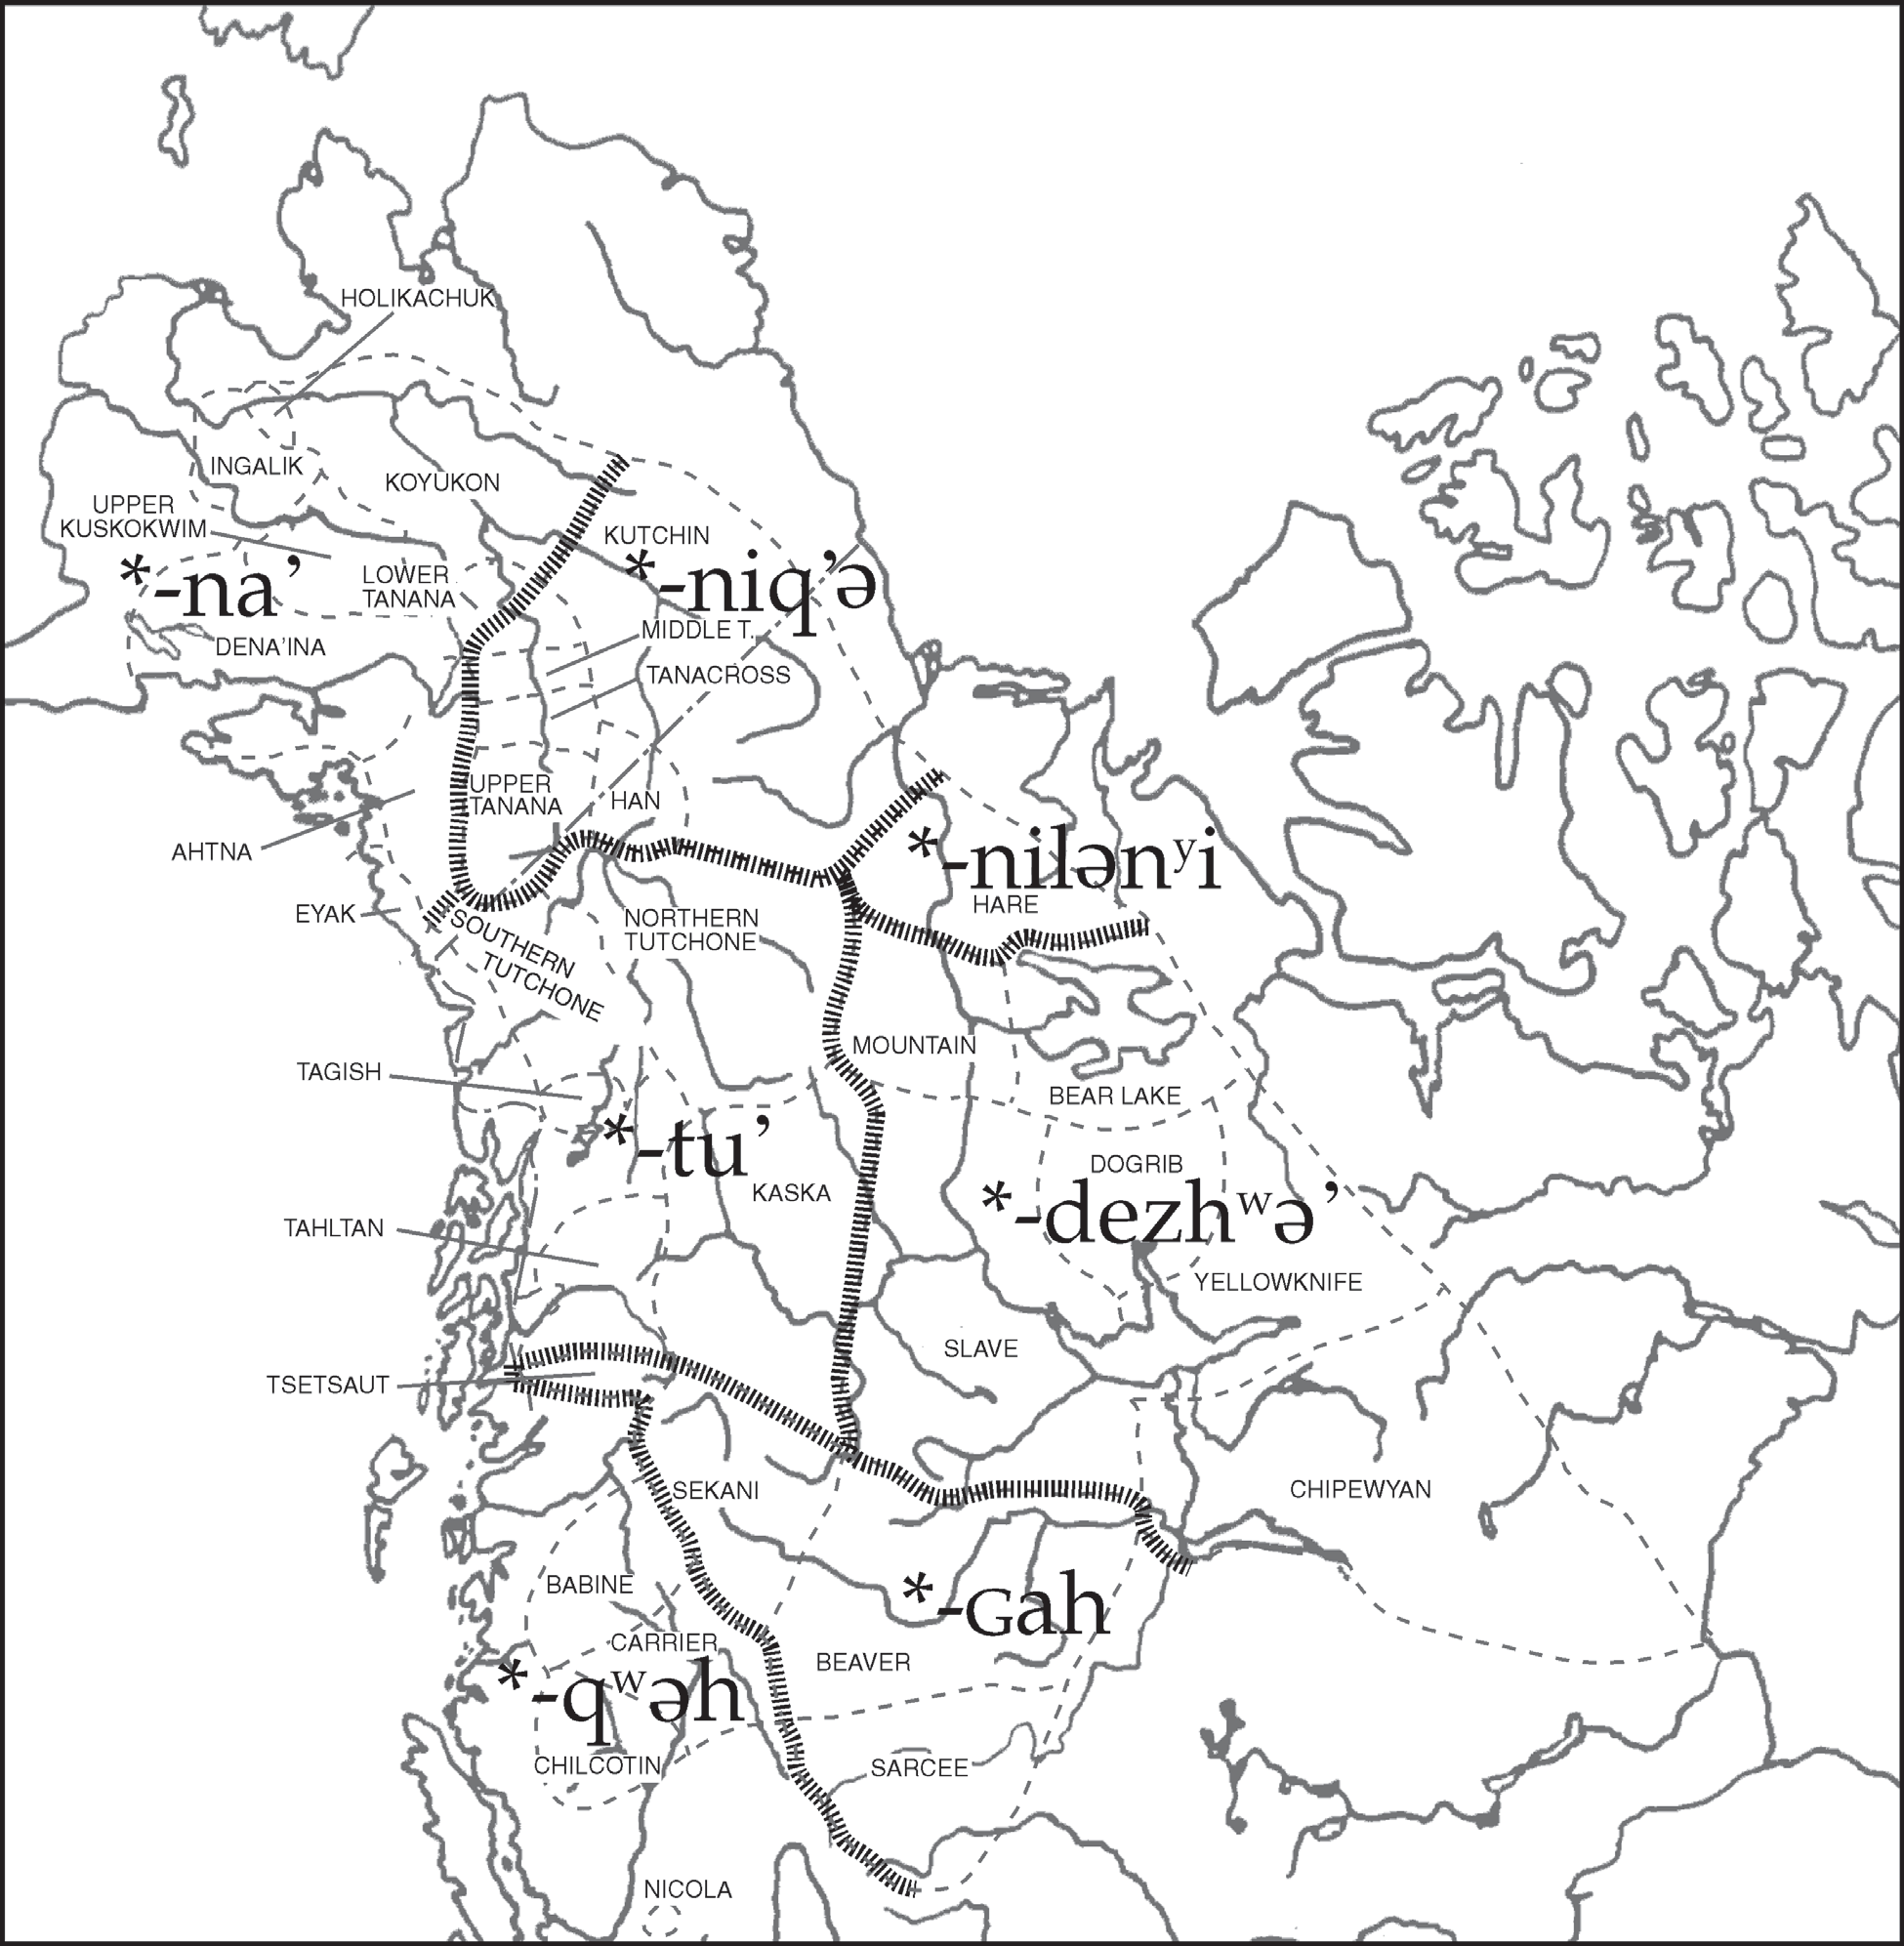
\includegraphics[width=0.7\textwidth]{figures/vajda-fig1}
\caption{Athapaskan hydronymic districts}\label{vajda-fig1}
\end{figure}


Only some of the river-name formants in Figure 1 have obvious etymologies (Kari 1996). Most of interior Alaska is divided into two hydronymic districts. The northeastern district is characterized by local reflexes of \textit{*–niq’ə}, which Kari etymologizes as meaning ‘upstream’. River names based on \textit{*–niq’ə} are in fact distributed upstream of river names belonging to the more western and southern Alaskan hydronymic district, characterized by the formant \textit{*–na}, a morpheme Kari relates to a verb root meaning ‘nomadize’. The etymologies of the two southernmost Canadian formants, \textit{*–qʷəh} and \textit{*–ɢah}, are not fully clear, though Kari (1996: 262) suggests they may have derived from morphemes meaning ‘along’ or ‘inside an enclosed space’. The formant \textit{*–nilənʲi} is unambiguously a nominalization of the verb root \textit{*lənʲ }‘current flows’; it also forms the only hydronymic district containing a single language (Hare). The formant \textit{*–deˑžʷə’}, found in river names across Arctic-draining areas of northwestern Canada, is the possessed form of Proto-Athapaskan \textit{*deˑšʷ} ‘sandbar, shoal, low island’. A cultural comparison with Yeniseian in Section 3 suggests a possible motivation for the semantic shift from ‘sandbar’ to ‘river’.

The western interior Canadian formant \textit{*–tu’} is the possessed form of the Proto-Athapaskan basic noun \textit{*tuˑ} ‘water’. Kari regards the area where the river-name formant \textit{*–tu’ }is prevalent as core Athapaskan territory, while formants used in other districts are likely to be later regional innovations (1996: 263-266). Harrington (1940) similarly viewed interior western Canada as some of the oldest territory occupied by Athapaskan speakers. Evidence for the primacy of \textit{*–tu’ }as a hydronymic formant comes from the fact that some river names in the other districts also have \textit{*–tu’}, whereas the remaining six formants are essentially limited to their respective districts as delimited in Figure 1.\textit{ }Kari (1996: 256) mentions the existence of four rivers in Ahtna territory with a final combining form \textit{*–tu’ }rather than \textit{*–na}, the typical formant for that area. The \textit{*–ɢah} district also contains river names in \textit{*–tu’}. Finally, in the Arctic-draining \textit{*–deˑžʷə’} district of northern Canada, \textit{*–tu’} ‘water’ regularly occurs as the final combining form in names of lakes rather than rivers (Kari 1996: 264).

Even if \textit{*–tu’} is indeed the original (or one of the original) Athapaskan hydronymic formants and the \textit{*–tu’} district is the nucleus from which the other districts later arose, the innovative formants \textit{*–na’}, \textit{*–niq’ə}, \textit{*–nilənʲi}, \textit{*–deˑžʷə’}, \textit{*–qʷəh}, and \textit{*–ɢah} still do not correlate with known sub-branches of the Athapaskan language family; it remains unclear how each became distributed across otherwise distinct linguistic boundaries. Concluding anything about the original Na-Dene hydronymic culture is made even more difficult by the fact that Tlingit and Eyak river-naming systems have not yet been systematically compared with Athapaskan. The Proto-Athapaskan nouns \textit{*deˑšʷ} ‘sandbar’ and \textit{*tuˑ} ‘water’ are cognate with the Eyak noun \textit{dehǯ }‘sandbar’ and Eyak preverb \textit{tu\textsuperscript{ʔ}}\textit{ }‘water’. The Tlingit nouns \textit{xág}\textit{\textsuperscript{w}} ‘sandbar’ and\textit{ héen} ‘water’ are used in complex Tlingit hydronyms (Thornton 2008: 56) but they do not appear to be cognate with any of the Athapaskan hydronymic formants discussed in Kari (1996). Because no shared system of toponymic morphology has yet been reconstructed even to the level of Na-Dene, any deeper comparison with Yeniseian river names must be limited, at least for the present, to identifying structural or semantic parallels rather than undertaking a genealogical comparison. Still, as will be argued below, a comparison of Dene-Yeniseian hydronymic nomenclature is illuminating for a number of reasons.

%section 2
\section{Yeniseian Substrate Hydronyms in Siberia}\label{vajda:sec:2}


The situation with respect to pre-Russian hydronyms in central Siberia differs from the traditional Athapaskan areas of North America is three salient respects. First, as already noted, Athapaskan hydronyms form ‘districts’ that cut across language boundaries, whereas the most common Yeniseian river-name formants display phonological traits connecting them to particular languages or branches of the family. Because Yeniseian hydronymic formants parallel established family-internal sub-divisions---and this is particularly true of river names built with final combining forms derived from Proto-Yeniseian \textit{*s\=es} ‘river’---they are of great value in tracing the prehistoric location of groups speaking particular Yeniseian daughter languages. Because the distribution of Athapaskan hydronymic formants do not match other known facts about the family’s historical diversification, they are not so readily helpful for tracing prehistoric population movements.

Second, the vast majority of recorded Yeniseian toponyms are specifically river names (potamonyms). Native Yeniseian names of lakes, hills, rocky outcrops, forest uplands, etc., survive only rarely in substrate areas; such toponyms were mostly recorded in territory still occupied by Yeniseian speakers when Russians initiated the first European contact after 1600. A logical reason for the overwhelming survival rate of substrate river names as opposed to other Yeniseian toponyms is proposed in Section 3 below. Most Yeniseian river names form substrate complexes that survive only through the medium of a second (if not a third) linguistic layer, and only a few were recorded directly from intact Yeniseian-speaking communities. By contrast, Athapaskan landscapes abound in toponyms naming the full gamut of natural geographic features. The fact that Athapaskan hydronyms were recorded by Jim Kari and other linguists directly from fluent native speakers, not merely by analyzing substrate relics left by long vanished populations, further contributes to the richness of the North American corpus in contrast to the much thinner record of Yeniseian toponyms in Siberia.

Finally, Athapaskan territory is saturated with native place names to the remarkable exclusion of any other layer of pre-European toponyms. This indicates either the family’s great age in the given territories, as argued in Kari (1996, 2010), or a strong cultural propensity to replace non-native place names in any newly acquired territory. The latter possibility is suggested by the fact that Navajo and Apache areas of the American Southwest, Athapaskan place names likewise blanket the landscape despite the known shallow time depth of occupation by Athapaskan speakers. to provide further insight into the link between toponymy and Athapaskan expansions, the Pacific Coast Athapaskan and Apachean areas should be compared with Northern Athapaskan. Whether due to time depth of occupation or cultural naming practices, or to both factors, Northern Athapaskan territory shows little or no sign of earlier linguistic substrates. Yeniseian-speaking peoples, on the other hand, were definitely only one ethnic component from among several known indigenous language families that contributed to the pre-Russian toponyms that survive today in south-central Siberia. Yeniseian substrate hydronyms are of great value in understanding ethnic and linguistic population replacements throughout south-central Siberia, a fact convincingly established by the great Siberian scholar Andreas P. Dulson (Dul’zon 1959). Most of the pioneering scholarship on Yeniseian toponyms by Dulson and other soviet era scholars appeared in local Siberian publications that are difficult to access. All of these important works, which number in the dozens, are listed in Vajda (2001: 372), where each is provided with a detailed English annotation.

The discussion below elaborates on the significance of these points of contrast between Yeniseian and Athapaskan river names: 1) the degree to which hydronymic formants match other known aspects of family-internal diversification, 2) the richness or poverty of the recorded toponymy, and 3) whether or not river names are interspersed with those of other language families.

\subsection{Hydronyms from Proto-Yeniseian \textit{*s\=es} ‘River’}

The Kets today live along the middle reaches of the Yenisei from the Mountain Tunguska north to the Kureika river, just above the Arctic Circle. As a nationality in the Russian Federation, they number 1209 people according to the 2010 census, although only a few dozen elderly people are fluent in any the three surviving dialects of the traditional language (Northern Ket, Central Ket, Southern Ket). When Russian fur traders and Cossack adventurers penetrated the Yenisei watershed in the decades following Yermak’s attack on the Khanate of Kuchum in 1582, the Ket hunting bands were only one of several linguistically distinct Yeniseian populations they encountered. Figure 2, redrawn from Vajda (2001: xxvii), shows the approximate distribution of Yeniseian-speaking groups as recorded in the 17\textsuperscript{th} century by Russian fur tax (\textit{yasak}) collectors. For more historiographic detail on Yeniseians in the first century after the Russians’ arrival, see Dolgikh (1960: 143-150, 184-191, 204-206, 222-275, and especially the back-cover foldout map insert). Present-day locations of Ket populations are marked in Figure 2 with stars.

\begin{figure}
\centering
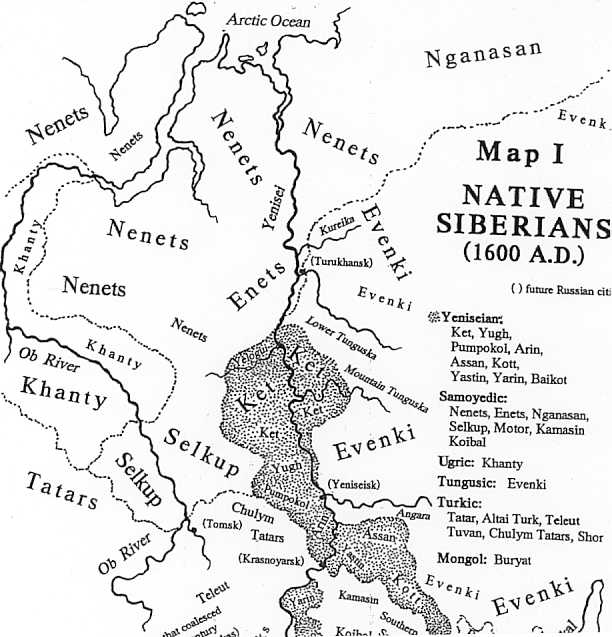
\includegraphics[width=0.7\textwidth]{figures/vajda-fig2}
\caption{Documented Yeniseian territories in 1600}
\label{vajda-fig2}
\end{figure}


Each language area shaded in gray contains river names with a formant reflecting Proto-Yeniseian \textit{*s\=es} ‘river’: Ket, –\textit{ses}, Yugh –\textit{čes},\textit{ }Arin –\textit{set}, Kott–\textit{šet }and Pumpokol\textit{ }–\textit{tet} (Werner 2005: 316-318). These variants show the regular reflexes of Proto-Yeniseian \textit{*s}, which yielded /t/ in Pumpokol and the sibilant /š/ in Kott (and in the closely related Assan). The final /t/ in Arin \textit{set} and Kott\textit{ šet }appears to have resulted from dissimilation of coda /s/ following an onset sibilant or shibilant. This type of dissimilation in Kott and Arin (but not Ket) is evident in at least one other item of basic vocabulary: Ket \textit{se’s} ‘larch (tree)’, but Arin \textit{čit} ‘larch’ and Kott-Assan \textit{šet} ‘larch’ (Werner 2005: 306). As for Yugh hydronyms, although the Ket and Yugh word for ‘river’ is \textit{s\=es}, the Yugh combining form is normally \textit{–čes}, in contrast to Southern and Northern Ket \textit{–ses} and Central Ket \textit{–šeš.} The change of syllable anlaut /s/ to /č/ in the middle of compounds also occurs sporadically in Northern Ket (cf. Southern Ket \textit{bənsaŋ} ‘it is not’, but Northern Ket \textit{bənčaŋ} \~{} \textit{bənsaŋ}).

Yeniseian-derived river names that survive as substrate toponyms among the current Russian- or Turkic-speaking populations of southern or western Siberia are built using virtually identical final combining forms that can easily be connected to a particular Yeniseian daughter language: \textit{–ses \~{} sis \~{} zis \~{} sas \~{} zes \~{} zas }(Ket), \textit{–čes }(Yugh), \textit{–set \~{} sat \~{} zet \~{} zat}, also\textit{ –kul }(Arin), \textit{–šet \~{} čet }(Kott), \textit{–ul }(Assan), \textit{–tet \~{} tat \~{} det \~{} dat }(Pumpokol). Variants such as \textit{zis \~{} sas} arose through accommodation to Turkic or other languages spoken by pastoral peoples who took over these areas. Alternation between /e/ and /a/ reflect the pattern of front/back vowel harmony typically found in the pronunciation of Turkic and most other Inner Eurasian languages, but lacking in the Yeniseian languages themselves.

Substrate river names with a final-combining form derived from PY \textit{*s\=es} ‘river’ are also distributed far beyond the areas documented by Russians as being inhabited by Yeniseian-speaking hunter-gatherers. Yeniseian river names are thus uniquely useful for tracing the former distribution and expansion of individual Yeniseian daughter languages. It is possible to postulate four distinct Yeniseian substrate zones based on known family-internal sub-divisions, as in \REF{vajda-substrate}.

%Table 1: Yeniseian substrate hydronymic zones based on reflexes of \textit{*s\=es} ‘river’

\begin{exe}\label{vajda-substrate}
\ex Yeniseian substrate hydronymic zones based on reflexes of \textit{*s\=es} ‘river’
\begin{xlist}
\ex Ketic \textit{*–ses} ({\textgreater}\textit{ ses \~{} šeš \~{} sis \~{} zis \~{} sas \~{} zes \~{} zas \~{} čes}) representing the known Ket dialects, as well as Yugh (\textit{čes}), and probably other closely related but otherwise undocumented language forms;
\ex Arinic \textit{*–set} ({\textgreater} \textit{set \~{} sat \~{} zet \~{} zat}) representing the documented Arin language and possibly other closely related but undocumented language forms;
\ex Kottic \textit{*–šet }({\textgreater} \textit{šet \~{} čet}) representing the documented Kott dialects, as well as Assan, though documented Assan potamonyms normally end in \textit{–ul} rather than a reflex of \textit{*–šet}), and possibly other closely related but undocumented language forms;
\ex Pumpokolic \textit{*–tet }({\textgreater} \textit{tet \~{} tat \~{} det \~{} dat}) representing the documented Pumpokol language and possibly other closely related but undocumented language forms.
\end{xlist}
\end{exe}

Figure~\ref{vajda-fig3} shows the location of \textit{*s\=es}{}-derived substrate hydronyms beyond the areas where 17\textsuperscript{th} century Russian fur tax collectors actually encountered Yeniseian-speaking groups (marked in gray, as in Figure 2). The placement of substrate hydronymic labels is unavoidably impressionistic. For example, if a 300-kilometer river carries a substrate Yeniseian name, it is not possible to know whether the original speakers nomadized along the river’s entire length or only near one location. Compact geographic clusters of a particular hydronymic formant, however, strongly indicate that speakers of a particular Yeniseian language variety once occupied the general area. Four hydronymic notations correlate with the four main documented Yeniseian daughter branches: Ketic (Ket-Yugh) \textit{ses}, Arinic \textit{set}, Kottic (Kott-Assan) \textit{šet}, and Pumpokolic \textit{tet. }Secondary phonetic variation (\textit{–zas, –sas}, \textit{–sis}, etc.), presumably caused by minor dialectal variation or adaptation into a superstrate language is ignored. The circled area is identified as the probable Proto-Yeniseian homeland, a proposal to be discussed in Section~\ref{vajda:sec:3}.


\begin{figure}
\centering
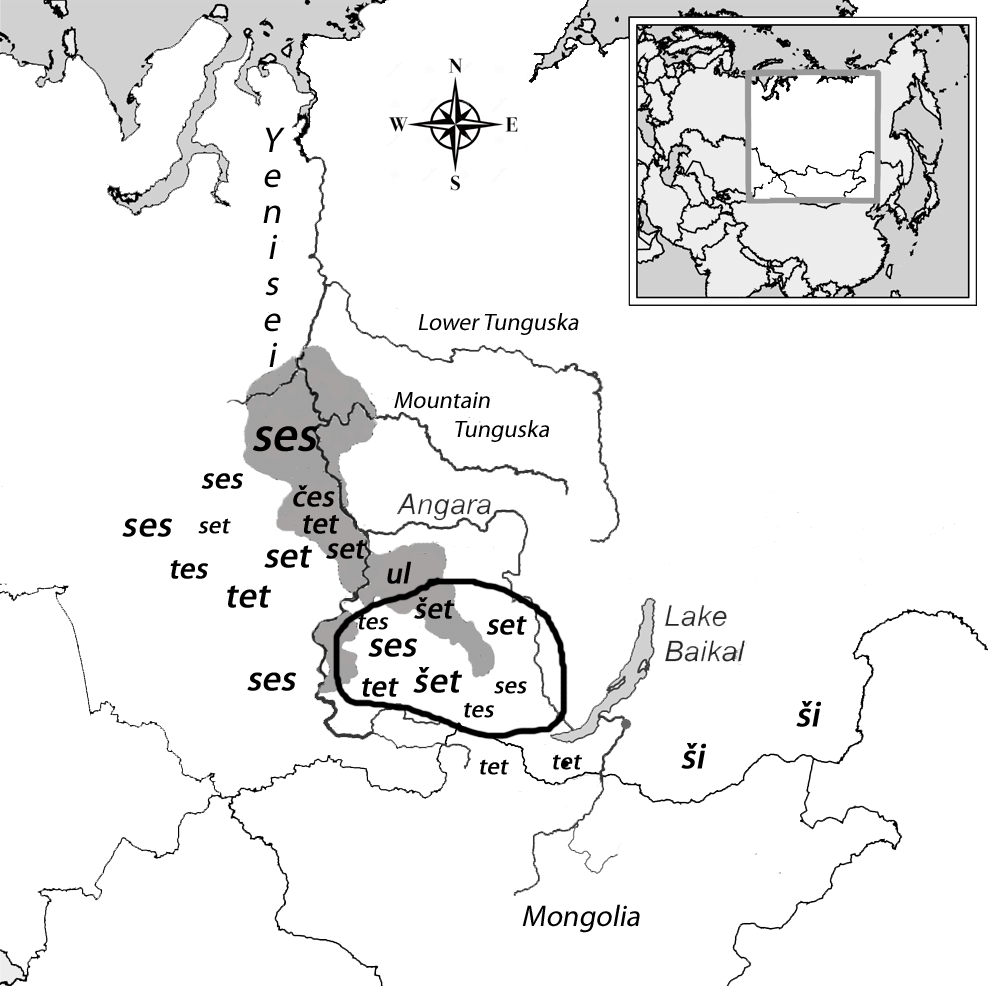
\includegraphics[width=0.7\textwidth]{figures/vajda-fig3}
\caption{Former distribution of Yeniseian languages shown by substrate toponyms}\label{vajda-fig3}
\end{figure}

%Figure 3: Former distribution of Yeniseian languages shown by substrate toponyms.



Two of the hydronymic notations in Figure~\ref{vajda-fig3}---\textit{tes} and \textit{ši}---do not correlate with any known Yeniseian language. They also plausibly derive from Proto-Yeniseian \textit{*s\=es} ‘river’ and may represent vestiges of extinct Yeniseian languages not otherwise documented. River names with the final combining form \textit{–tes \~{} tas \~{} tɨš} \textit{\~{} des \~{} das }appear in large areas of south and western Siberia. If these river names do reflect evolution from PY \textit{*s\=es} ‘river’, as originally proposed by Dul’zon (1959), then the initial plosive /t \~{} d/ could conceivably have arisen in any of several ways. Such a Yeniseian daughter language may have undergone a secondary dissimilation of anlaut /s/ to /t/ in syllables ending in a sibilant (\textit{*s\=es} {\textgreater} \textit{tes}). In that case, the \textit{*–tes }river names would probably form an extension of the Ketic zone. Or, alternatively, the final combining forms \textit{–tes \~{} tas \~{} des \~{} das} might preserve the Yeniseian 3\textsuperscript{rd} person possessive connector prefix \textit{d}{}- (\textit{*d-s\=es} {\textgreater} \textit{tes}), though this morphological trait is not observed in river names associated with known Yeniseian languages. The most intriguing possibility is that the original Proto-Yeniseian form of ‘river’ may have been \textit{*tes} or \textit{*des} rather than \textit{*s\=es}, with initial /s/ in all documented languages arising from long distance sibilant assimilation (\textit{*tes }or\textit{ *des} {\textgreater} \textit{ses},\textit{ set}, etc.). This would make the earliest Yeniseian word for ‘river’ resemble Proto-Athapaskan \textit{*deˑšʷ} and Eyak \textit{dehǯ}. However, the possibility that long distance anlaut sibilant assimilation yielded \textit{*s\=es} from earlier \textit{*d\=es} in the language ancestral to Ket appears to be contradicted by the fact that no such assimilation occurred in phonologically similar words (cf. Southern Ket \textit{d\=es} ‘eye’, \textit{tòs} ‘raising’, \textit{do’s} ‘anthropomorphic spirit image fashioned from a log’, etc.). Most \textit{*–tes }river names are found in southern or western Siberia, though one is located in northern Ket territory: the Luntes tributary of the Kureika river. “Luntes” appears to derive from \textit{l\=un} ‘grayling (fish)’ + \textit{s\=es} ‘river’ via deaffrication of original \textit{lun-čes}. It is not connected with the more numerous south and west Siberian river names of undetermined linguistic provenance (Kajtes, Baktas, Kɨtas, Utaz, etc.), though it is possible that the final combining form in these names too could have arisen through secondary affrication and deaffrication in whatever Yeniseian language or dialect they derive from. The example provided by the river name “Lunches” demonstrates how the presence of a single substrate toponym can generate ambiguous conclusions. Areas with multiple examples of the same morphological type of substrate toponym are more useful in exploring linguistic prehistory. Dulson’s identification of a Yeniseian origin (Dul’zon 1959) for river names in \textit{–tes \~{} tas \~{} tɨš} \textit{\~{} des \~{} das }in southern and western Siberia (conceivably including the name of the large Irtysh river), remains the most plausible interpretation. These toponyms form compact zones and the initial combining forms in some of them appear to have Yeniseian etymologies (Maloletko 2002: 152-154; Werner 2002, vol. 3: 68-69). These two facts make it unlikely that all southern and western Siberian \textit{–tes }river names arose through random secondary affrication followed by deaffrication, as occurred in the solitary case of Northern Ket “Luntes”.

River names ending in \textit{–ši \~{} či} found in southeastern Siberia may also reflect PY \textit{*s\=es} ‘river’, though in no recorded Yeniseian language does the final consonant of this formant elide. Many \textit{–ši }river names are found across Zabaikalye, well to the east of Lake Baikal and extending as far as Heilongjiang (formerly Manchuria) and the Amur basin (Zhamsaranova 2015); they appear to be widely distributed in these territories, which were occupied by Buryat Mongols or Ewenki (Tungusic) pastoralists when Russians penetrated the area. The possibility of Yeniseian river names in eastern Siberia, closer to the Pacific, is intriguing for understanding the geography of the Dene-Yeniseian connection, but more work needs to be done to strengthen the case that toponyms in \textit{–ši} are, in fact, of Yeniseian linguistic origin.

\subsection{Yeniseian River Names Without \textit{*s\=es}}

Interspersed across areas containing Yeniseian hydronyms built with \textit{*s\=es} ‘river’ are other Yeniseian river names built using completely different formants. Chief among these are river names containing reflexes of Proto-Yeniseian \textit{*x\=ul} ‘water’. These are particularly prevalent in the Assan areas (Werner 2002 vol. 3: 61-64), where the final combining form \textit{–ul} (less often rhotacized to \textit{–ur}) appears more frequently than Kottic \textit{–šet}. This pattern correlates with 18\textsuperscript{th} century word lists, where the free form \textit{ul} (rather than \textit{šet}) is recorded as meaning both ‘river’ and ‘water’ in Assan (Werner 2005: 144). The final combining form \textit{–kul} in river names correlates with Arin, and also matches the Arin free noun \textit{kul} ‘water’. Arin river names in \textit{–kul} tend to occur in the same general areas as Arin river names in \textit{–sat}. The reason behind the difference in morphological formant is unclear. Yugh \textit{\=ur} ‘water’ also shows up occasionally in Yugh territory river names as the final combining form \textit{–ur}. River names ending in \textit{–ur }are also found in south Siberia east of Lake Baikal (Zhamsaranova 2015), including the same areas containing the possibly Yeniseian-derived river names in \textit{–ši}. Hydronyms ending is a syllable with the shape \textit{–ur} are also well represented in the Amur watershed stretching eastward to the Pacific, and include the name ‘Amur’ itself, though there is no evidence that any of them are connected with Yeniseian \textit{*x\=ul} ‘water’. It is difficult to etymologize the internal structure of east Siberian \textit{–ur} hydronyms or identify any of them as Yeniseian in the absence of additional evidence showing that Yeniseian-speakers lived that far east of Lake Baikal. Yeniseian hydronyms that are fully etymologizable most often name some economically salient feature of the riverine environment, such as the type of fish, plant or animal found there and transparently conform to the structure: modifier noun (or adjective) + head noun. The initial portions of the various eastern Siberian –\textit{ur} river names cannot at present clearly be identified with specific Yeniseian words.

Many areas of south and west Siberia that contain river names with unambiguous reflexes of PY \textit{*s\=es} ‘river’ or \textit{*x\=ul} ‘water’ also contain river names ending in \textit{–kat }(or its substrate phonetic variants \textit{–ket} \~{} \textit{gat} \~{} \textit{get}) or \textit{–lat }(or \textit{–let}). Werner (2012) has argued persuasively that \textit{–kat \~{} ket }originated from a Proto-Yeniseian root meaning ‘clan’ (cf. Modern Ket \textit{kə’t} ‘children of the same mother’ and Kott \textit{kat} ‘children’). This also explains why \textit{–kat }\~{} \textit{ket} \~{} \textit{gat} \~{} \textit{get} river names are found primarily in areas alongside either Ketic \textit{–ses} or Kottic \textit{–šet}. Presumably, such names derived from ethnonyms of Yeniseian-speaking kin groups who nomadized near the given river and who met and traded there with other nationalities, thus transferring their clan designation to an alien linguistic community as the name of the given river.

This analysis can further be extended to river names with the formant \textit{–lat }\~{} \textit{let}. These appear to have the same etymology, but reflect Arin and Pumpokol phonology: cf. Arin \textit{alpolat} ‘child’ and Pumpokol \textit{hiluŋla} ‘child’, where the final syllables \textit{{}-lat} and \textit{{}-la} are cognate with Ket \textit{kə’t} ‘children of the same mother’ and Kott \textit{kat} ‘children’. The odd sound correspondence Ket /k/, Kott /k/, Arin /l/, Pumpolkol /l/ occurs in other words, as well, such as the noun ‘winter’: Arin \textit{lot}, Pumpokol \textit{lete}, Kott \textit{kêti}, Southern Ket \textit{kət}.

Other river names derive from words having to do with nomadizing. \ The geography of the seasonal nomadic cycle is similarly reflected in Ket river names ending in \textit{–kaŋ}, which are derived transparently from the Southern Ket noun \textit{kàŋ }‘winter hunting trail’. These tend to be small, upland tributaries, especially those in the Mountain Tunguska watershed, along which Kets traveled during their winter hunting forays, whereas \textit{–ses} names larger rivers where Ket families camped during the warm season; see Werner (2002, vol. 3: 34-42) for a list of \textit{–kaŋ} tributaries interspersed with \textit{–ses} river names. The use Southern Ket \textit{kàŋ }‘winter hunting trail’, a morpheme associated with nomadizing, as a river name formant finds a semantic parallel in the Alaskan Athapaskan hydronym formant \textit{*–na}, if the latter is indeed connected with verb forms meaning travel in a group.

Areas with river names in Ketic \textit{–ses }or\textit{ –kat}; Kottic \textit{–set}, \textit{–kat }or\textit{ –ul}; Arinic \textit{–set}, \textit{–kul }or\textit{–lat}; and Pumpokolic \textit{–tet} or\textit{ –lat} also contain a scattering of river names built with the element \textit{–tɨm \~{} tom}. The tom river, on which the eponymous city of tomsk is located, also belongs in this group. The tomsk area falls inside the Pumpokolic substrate zone, and in fact the word \textit{tom} in 18\textsuperscript{th} century Pumpokol word lists is glossed as ‘river’. Although the basic Proto-Yeniseian noun for ‘water’ is \textit{*x\=ul}, with reflexes in every daughter language, there is some evidence that a root with a form something like \textit{*to \~{} tu \~{} tom }also meant ‘water’ in Yeniseian. In addition to substrate river names in \textit{–tɨm \~{} tom} found in areas representing all of the documented Yeniseian daughter branches, Ket and Yugh have a number of complex word containing this morpheme in the meaning ‘water’. These include: Ket \textit{t\={o}ˑgde} ‘river bend’, ‘small bay in river’ {\textless}\textit{ to }‘water’ + \textit{ged }‘bend’; Ket \textit{tɨmoks}\textbf{\textit{ }}‘wood shavings used for cleaning of dishes {\textless}\textbf{\textit{ }}\textit{tɨm }‘water’ + \textit{\={o}ˑks }‘wood’; Ket \textit{toʁ\'{o}jiŋ}, Yugh \textit{toχojiŋ }‘drying’ {\textless} \textit{to }‘water’ + \textit{qoj }‘dry’ + \textit{ŋ }(action nominal suffix); Ket \textit{totaləŋ}, Yugh \textit{totarɨŋ }‘shallow’ {\textless} \textit{to} ‘water’ + \textit{tol} ‘low’ + \textit{ŋ} (adjective suffix); Central Ket dialectal \textit{tɨmet} ‘lake’ {\textless} \textit{tɨm} ‘water’ + \textit{et }‘surface (?)’; and Central Ket dialectal \textit{tamtul} ‘lake’ {\textless} \textit{tɨm} ‘water’ + \textit{tul} ‘cavity, bottom, low area’. The alternation between nasal and non-nasal codas in \textit{to \~{} tu \~{} tom \~{} tɨm }is unexplained and complicates the obvious suggestion of cognacy with Proto-Athapaskan \textit{*tuˑ} ‘water’, which shows no nasal coda in any modern Athapaskan dialect (Vajda 2010: 81). Also complicating the Dene-Yeniseian comparison is the fact that the most prevalent Yeniseian word for water is clearly \textit{*x\=ul}, which does not seem to have a cognate in any Na-Dene language.

The largest rivers in the Ket areas, which represent the most northern portions of Siberia known to have ever had Yeniseian-speaking inhabitants, are not built with any of the formants typically found in Yeniseian names for smaller tributaries (\textit{–ses}, \textit{–tɨm}, \textit{–ul}). The Yenisei river itself is called \textit{q\=uk}, a name with no clear etymology; see Janhunen (2009: 73-74) for a cogent discussion of the origins of various ethnic designations for the Yenisei river. The term is more likely to be a substrate hydronym of unknown origin than the result of polysemy from the homonymous Ket noun \textit{q\=uk} ‘hole, perforation’. Ket folk etymology associated the native name for the Yenisei with the hole that the great shaman Doh created in a rock cliff. This allowed the Yenisei to flow northward, giving the Ket people a route of escape from the malevolent female deity Hosedam. The Kets also refer to the Yenisei using the descriptor \textit{\=uls }‘wide expanse of water’ ({\textless} Pre-Ketic \textit{*\=ul} ‘water’ + \textit{*wes} ‘open space’), but this is not a proper noun uniquely applied to the Yenisei, as it can be applied to any broad expanse of water.

The large eastern tributaries of the Yenisei, which flow down from the Central Siberian Plateau, have names mainly built with \textit{qol \~{} qo’l}. These include \textit{Qo’l} or \textit{Qaʁol }‘Mountain (or Stony) Tunguska’ ({\textless} \textit{qà }‘big’ + \textit{qo’l}), as well as \textit{Baŋnoqol} ‘Lower Tunguska’, \textit{Boɣenol} ‘Dry Tunguska’. The latter two names may have the initial combining form \textit{ba’ŋ }‘earth’, referring to rapids and swiftly moving water; cf. Ket \textit{bannej} ‘splashing of water against objects’, \textit{baŋes \~{} baŋnas }‘rapids’ {\textless} \textit{*ba’ŋ} ‘earth’ + \textit{*wes} ‘open space’. These are turbulent rivers that descend at a steeper gradient than the low-lying western tributaries of the Yenisei. Therefore, the formant \textit{qol} is unlikely to have derived polysemously from Ket \textit{qo’l }‘calm water, small bay’ ({\textless} \textit{*q\={u}g}\textbf{\textit{ }}‘calm’ + *\textit{\={u}l} ‘water’). Also unexplained are the Yeniseian names for the Bakhta river: Ket \textit{Baqtoq}, Yugh \textit{Beaχtaχ}, which are unlikely on phonological grounds to contain \textit{*to} ‘water’ as their final combining form. More likely, the shape of these names represent a form originally ending in the syllable \textit{–qol}, which has reduced to coda /q/. This is unproven but would be in keeping with the fact that the Bakhta is also an eastern tributary of the Yenisei, draining from the same Central Siberian Plateau as other river names with the final combining form \textit{–qol}.

Finally, a number of river names, mostly in Yugh territory, are built with the syllable \textit{sɨm}. These include the Sym river itself and some of its tributaries (Werner 2002, vol. 3: 42-44). River names with final combining form –\textit{sɨm} reflect a pre-Yeniseian substrate of unknown origin, since the anlaut /t/ in the Yeniseian formant\textit{ –tɨm} would not have become /s/ in Ket or Yugh. Alekseenko (1975) suggested that river names with \textit{sɨm} were left by the original Yugh tribe, who did not speak a Yeniseian language and whose ethnic designation was transferred to the Ketic-speaking bands who later moved into this area and became known as the “Yugh” or “Sym-Ket”. The prevalence of major non-Yeniseian hydronyms in the lands that Ket and Yugh people actually inhabited during the historic period can be explained by the relatively recent migration of Ket and Yugh family groups from more southerly areas. These migrations are well attested in Ket folklore (Alekseenko 1967), early Russian fur tax records (Dolgikh 1960), as well as on modern maps by the presence of many \textit{–ses} river names in areas far to south or west of today’s Ket villages located in the north of the modern Turukhansk District in Krasnoyarsk Krai (Dul’zon 1959).


\section{Hydronyms and the Dene-Yeniseian Connection}\label{vajda:sec:3}

Before turning to a morphological comparison of Yeniseian and Athapaskan river names, it would be useful to mention the existence of a small number of Yeniseian toponyms naming other geographic objects and consider why the names of small to medium-sized rivers are so overwhelmingly prevalent in Yeniseian substrates in contrast to other toponyms.

Lake names in Ket-Yugh areas often end in the formant \textit{–de}, derived transparently from the Ket and Yugh noun \textit{de’} ‘lake’: Ket \textit{Dɨnde} {\textless} \textit{dɨn} ‘spruce’ + \textit{de’} ‘lake’, \textit{tomulde} {\textless} \textit{t\=um} ‘dark’ + \textit{\=ul} ‘water’ + \textit{de’} ‘lake’. The names of small streams in the Ket areas (in contrast to rivers) sometimes contain the final combining form \textit{–qoks}, from the noun \textit{qoks} ‘stream, brook’, less often \textit{–doks}. The final \textit{{}-s} in\textit{–qoks} and \textit{–doks} resembles the nominalizing suffix \textit{*-si}, which would suggest that \textit{*qok} and \textit{*dok} were verbal roots (cf. the Ket verb base\textit{ -doq} ‘jump, spring, fly’). Wooded uplands often carry names ending in \textit{–lɨt}, from \textit{lɨ’t }‘forest, forested upland’, such as \textit{qonlɨt} {\textless} \textit{qo’n} ‘fir, conifer’ + \textit{lɨ’t }‘upland’, \textit{qoqŋlɨt} {\textless} \textit{qokŋ} ‘pine forest’ + \textit{lɨ’t }‘upland’. While there are no true mountains in the northern Ket areas, the Shor district just north of the Altai preserves a few substrate oronyms (mountain names) with the final combining form –\textit{sai}, probably correlating with Kott dialectal \textit{džii} \~{} \textit{gijlin} ‘mountain(s)’ (Werner 2005: 310). These forms reflect Pre-Kottic *\textit{ǯi:l} (plural\textit{ *ǯi:l-in}), a probable cognate of Proto-Athapaskan \textit{*ʒəł} ‘mountain’ and Tlingit \textit{gudl} ‘mound, hump’. Athapaskan uses reflexes of \textit{*}–\textit{ʒəł} in naming mountains above the timberline. It is possible that Pre-Ketic \textit{*lɨ’d}\textit{\textsuperscript{j}} ‘upland’ is a metathesized form of earlier \textit{*d}\textit{\textsuperscript{j}}\textit{ɨl} ‘mountain’, given the prevalence of innovative metathesis in Ket-Yugh and its relative absence in Kott-Assan. The Ket formants \textit{–qoks} and \textit{–doks }are not obviously cognate with Na-Dene toponymic elements.

Except for river names, very few Yeniseian toponyms survive in substrate areas. Outside the modern Ket areas, river names account for the vast majority of substrate Yeniseian geographic terms, far outweighing in number all other types of toponyms. The reason for this is likely connected with the traditional Yeniseian hunter-gatherer economic lifestyle (see Alekseenko (1967: 37-79) for the classic description), including patterns of when and where Yeniseians typically interacted with speakers of other languages. In winter months the Kets traditionally broke up into small family groups, each moving separately upland from the river’s edge to nomadize in the forests. Each family band typically traveled along a small tributary upland from one of the larger rivers, hence the existence of river names in \textit{–kaŋ} ({\textless} \textit{kàŋ} ‘winter hunting trail’). In spring, the Kets would migrate back to the larger rivers, regrouping with other family bands to camp at the water’s edge. Rivers with sandy margins were favored over swampy riparian zones where vegetation grew down right into the water. Sandy riverbanks made good foundations for birchbark teepees and were exposed to breezes that helped disperse the clouds of biting insects.

The same ecological considerations probably motivated the derivation of the north Canadian Athapaskan river name formant \textit{*–deˑžʷə’} on the basis of Proto-Athapaskan \textit{*deˑš} ‘sandbar’. It is possible that Proto-Athapaskan \textit{*deˑšʷ} ‘sandbar’ and Eyak \textit{dehǯ }‘sandbar’ could be ancient nominalizations created by a possessive prefix \textit{d-} attached to Proto-Athapaskan *\textit{sa:x}\textit{\textsuperscript{y}} ‘sand, gravel’ (cognate with Tlingit \textit{xágʷ} ‘sandbar’), or to Proto-Athapaskan \textit{*səx} ‘small particles’, which Vajda (2010: 82) identified as cognate to Yeniseian \textit{*six} ‘small bits’. Deriving Proto-Athapaskan \textit{*deˑšʷ} and Eyak \textit{dehǯ }‘sandbar’ from a nominalization like \textit{*də-səx }‘something made of small particles’ or \textit{*də-sa:x}\textit{\textsuperscript{y}}\textsuperscript{ }‘something made of sand, gravel’ remains speculative, however.

It is tempting to see the same semantic shift from ‘sand’ to ‘river’ in the Yeniseian word \textit{*s\=es} ‘river’. Despite its superficial resemblance to Proto-Athapaskan *\textit{sa:x}\textit{\textsuperscript{y}} ‘sand, gravel’, however, Proto-Yeniseian \textit{*s\=es} means ‘river’, never ‘sand’, in every Yeniseian language. PY \textit{*s\=es} ‘river’ could conceivably have derived from a Pre-Proto-Yeniseian nominalization of \textit{*six} ‘small bits, particles’ + \textit{*si} (nominalizing suffix). The root \textit{*six} gives the Ket-Yugh initial combining form \textit{si- }‘small bits’ in several compounds, including\textit{ }Ket \textit{si-kit} ‘sweep’ (\textit{k\=\it} ‘rub’) and Ket \textit{siis}, Yugh \textit{sifes }‘pile of small bits’\textit{ }(\textit{*pis }‘pile’). Modern Ket and Yugh, however, use unrelated words for ‘sand’: Ket \textit{hənaŋ} ‘grains of sand’ {\textless} \textit{*pən} ‘small’ + *\textit{ŋ }(collective noun suffix) and Ket \textit{qe’s}, Yugh \textit{χe’s} ‘sandbank’ (origin unclear). There is no morphological evidence linking the etymology of PY \textit{*s\=es} ‘river’ to Yeniseian words for ‘sand’ or ‘sandbank’, though the semantic connection is logically possible.

Regardless of the ultimate morphological origin of PY \textit{*s\=es} ‘river’, the overwhelming preponderance of Yeniseian river names can be explained on ethnological grounds. If the early 20\textsuperscript{th} century lifestyle of the Ket people can be taken as characteristic, Yeniseian hunter-gatherer bands generally met to interact peacefully with other nationalities at sandy riverbanks in the warm season. It was during these interactions that Yeniseian names for river (\textit{*}–\textit{ses}), water (*–\textit{tɨm}, \textit{*–xul}), kin group (–\textit{kat}, –\textit{lat}), or nomadizing trail (\textit{–kaŋ}) were transmitted to speakers of alien languages, eventually becoming substrate toponyms on modern maps of Siberia. Because summer river encampments were the favored place for peaceful multi-ethnic interactions, river names were the most frequent Yeniseian toponyms adopted by pastoral peoples who supplanted Yeniseian speakers throughout much of their former range.

\subsection{Hydronymic Evidence for a Yeniseian Homeland in South Siberia}


Numerous substrate river names of Yeniseian linguistic origin distributed across broad areas of Siberia add greatly to our understanding of the area once inhabited by Yeniseian-speaking tribes. The study of Ket-related hydronyms significantly extends what can be deduced about the location of Yeniseian speakers prior to the historic period, which began with Russian fur tax (\textit{yasak}) records dating from the early 1600s (Dolgikh 1960). Nearly all of this territory was taken over by pastoralists speaking Ugric (mainly Eastern Khanty), Samoyedic (southern Selkup dialects, as well as Mator and Kamassian---extinct languages of the Altai-Sayan region), Turkic (Northern Altai, Chulym, Khakas, Tuvan, tofan, as well as West-Siberian Tatar dialects), Tungusic (Western Evenki dialects), or Mongolic (mainly Buryat). Replacement of Yeniseian-speaking hunter-gatherers by Uralic or Altaic pastoralists across south Siberia must have begun over two millennia ago. The fact that the known Yeniseian daughter languages are clearly distinguishable in the substrate toponymy of southern Siberia means that Proto-Yeniseian must have already broken up into distinct Ketic, Kottic, Arinic and Pumpokolic daughter branches prior to the arrival of pastoral tribes. How much earlier the breakup of Common Yeniseian predates pastoralism in the Siberian forest-steppe and taiga zones cannot be ascertained from verifiable historical events. Because the known Yeniseian languages do appear rather closely related, their divergence is unlikely to have been many thousands of years earlier. Based on the degree of similarity between the documented Yeniseian languages, a rough guesstimate for the breakup of Common Yeniseian might be three, possibly four thousand years ago.

Yeniseian hydronyms in North Asia, at least in the sub-Arctic areas of their distribution, clearly overlay earlier systems. Interspersed with the Yeniseian are layers of Ugric, Samoyedic, Turkic, and Tungusic place names of various sorts (Dul’zon 1959). Many river names show layering of morphemes from more than one of these families (Dul’zon 1959, Maloletko 2002). Only in the area of south-central Siberia between Lake Baikal, northern Mongolia and the Upper Yenisei basin are Yeniseian river names showing the full extent of known family-internal diversity found in compact profusion. Substrate toponyms demonstrate early occupation of this general area by all known Yeniseian daughter branches. The homeland, or rather the dispersal point of the documented Yeniseian languages, is likely to be found in this part of south central Siberia or some adjacent territory.

While the linguistic facts suggest that the diversification and spread of the documented Yeniseian languages in North Asia probably date back no farther back than three or four thousand years, they say nothing in themselves about the age of Yeniseian presence in Siberia or about its earlier origin. Maloletko (2002) suggests the Yeniseians in prehistory migrated from southwest Asia, near the Caucasus or present-day Turkey. There is no evidence, however, either from ethnography or human genetics, to suggest that the ancestors of Yeniseian-speakers first appeared in Siberia only a few thousand years ago from such a distant point of origin. On the contrary, evidence from human genetic studies support the probability that many, if not most, of the physical ancestors of today’s Ket-speaking population inhabited south Siberia as far back as the Middle Holocene if not deeper into the Early Holocene or Late Pleistocene. Modern Ket males overwhelmingly (\~{}95\%) belong to Y-chromosome haplogroup Q, shared distantly with most Native American males, though not more closely with Athapaskans than with Native Americans speaking languages from unrelated families (Scott and O’Rourke 2010: 132-133). The Kets are the only Old World ethnic group, together with neighboring Selkups (\~{}63\% Q haplogroup) to have this genetic profile on the male line (Starikovskaya et al. 2005; Karafet et al. 2008). Ket females show a mixture of western and eastern Eurasian mt-DNA haplogroups that is unique in modern North Asia. Ket mt-DNA includes eastern haplogroups A and C together with the ancient west Eurasian haplogroup U5a, as well as a significant percent (27.7\%) of haplogroup F (Starikovskaya et al. 2005: 78), found in no other modern North Asian population in more than trace amounts (Karafet et al. 2008). A similar mixture of Mt-DNA haplogroups, including nearly 50\% mt-DNA haplogroup F, now mostly absent in North Asia outside the Ket population, was detected in two hunter-gatherer burials dating back to the Middle Holocene (7,000 to 6,000 years ago) near the southern tip of Lake Baikal (Schurr et al. 2010). This offers strong circumstantial evidence that the physical ancestors of the Kets, at least on the female line, were ancient residents of South Siberia and not newcomers. The same general areas of south-central Siberia that contains Yeniseian substrate hydronyms also have been found to contain a complex of six folklore motifs uniquely shared with the Na-Dene peoples of North America (Berezkin 2015). These motifs were collected from the traditional folklore of south Siberian Turkic- and Uralic-speaking peoples containing a Yeniseian cultural substrate, but not documented in the actual folklore of northern Ket and Yugh speakers themselves. Berezkin surmises that the Ket lost some of their characteristic south-Siberian boreal folklore when moving north into the circumpolar region.

Yeniseian hydronyms found in western Siberia and sub-Arctic central Siberia clearly overlay other linguistic systems. Areas with Ket or Yugh populations during the past four hundred years retain significant linguistic substrates, including river names based on \textit{sɨm} and \textit{qo’l}---river name formants of undetermined origin. Only in certain parts of south-central Siberia are Yeniseian hydronyms found in enough profusion and family-internal phonological diversity to suggest early habitation by Yeniseian-speaking groups. The evidence suggests an expansion of the Yeniseian daughter languages from a south-Siberian homeland somewhere roughly between the upper reaches of the Yenisei, northern Mongolia and the southern tip of Lake Baikal.

\subsection{South Siberian Hydronyms in \textit{–man}}

One final possible connection between south Siberian hydronyms and those of the Athapaskan areas of North America remains to be discussed. Dul’zon (1962) analyzed over 150 hydronyms built with the formant \textit{–man }(less often\textit{ man}\textit{\textsuperscript{y}},\textit{ men},\textit{ ben},\textit{ ven}) in the forest-steppe and southern taiga zones stretching from north of the Amur all the way across Inner Eurasia to the Volga River region in Eastern Europe. These hydronyms name either lakes or rivers across this wide area and appear to predate Turkic, Indo-European, Uralic, Samoyedic languages. Because the linguistic origin of river and lake names in \textit{–man }has never been explained, it is worth mentioning their superficial similarity to Proto-Athapaskan *\textit{mən} ‘lake’. Reflexes of this root, sometimes with a possessive suffix -\textit{ə’} (*\textit{–mənə’}) appear as the primary final combining form of lake names across four of the six northern Athapaskan hydronymic districts (Kari 1996: 256-259), except in the \textit{*–nilənʲi} and \textit{*–deˑžʷə’ }districts, where reflexes of \textit{–tu’} ‘water’ have come to serve as the primary lake name formant instead. Even if South Siberian river and lake names in \textit{–man }were left by the ancestral cousins of the Na-Dene, it is still not clear whether there is a genealogical connection with Yeniseian hydronymic systems. Ket lake names always end in –\textit{de}, never \textit{–man}, and there is no evidence of any Yeniseian morpheme cognate with Proto-Athapaskan *\textit{mən} and Eyak \textit{maˑ} ‘lake’. Also, the mysterious Siberian \textit{–man} hydronyms are more often river names than lake names, whereas North American Athapaskan *\textit{–mən \~{}} *\textit{–mənə’} hydronyms are exclusively lake names. Finally, \textit{–man} hydronyms appear to form an even earlier substrate inside of Yeniseian hydronymic districts, being overlaid by Yeniseian formants such as Kottic \textit{–šet} or Pumpokolic \textit{–tet} in river names such as Kumanshet, Tumandat, etc. All of these factors complicate recognizing –\textit{man} hydronyms as evidence for the Dene-Yeniseian connection. Nevertheless, the possibility that these river and lake names form a direct toponymic link between Siberia and Native America is at least worth considering in the absence of a better explanation. Dulson suggested that the Ancient Turks spread \textit{–man} hydronyms westward, though he also claimed that the hydronymic formant \textit{–man} itself is etymologically not of Turkic origin, as it is also found in areas of southeastern Siberia where no Turkic groups ever lived (Dul’zon 1962). The origin of south Siberian \textit{–man} hydronyms therefore remains undetermined, though their connection with the early origin of Na-Dene speakers in Inner Eurasia is not implausible. The area of \textit{–man} hydronyms in south Siberia also coincides with the area where Berezkin (2015) found folk motifs connecting southern Yeniseian substrates with the Na-Dene.


\subsection{Yeniseian and Na-Dene river-oriented directional morphology}

Both Yeniseian (Vajda 2013) and Na-Dene (Leer 1989; Fortescue 2010: 44-53) contain well-developed morphological systems to specify direction in regard to a fixed location such as a river or other body of water. Leer (1989: 576) used the term ‘directionals’ to refer to these morphemes in Na-Dene, but the term is no less apt for Yeniseian. Directionals can appear as possessed nouns, object of postpositions, or incorporate into motion verbs. Yeniseian directionals have the same functional range. The examples in \REF{vajda-ex1} contain complex Ket directional constructions, where a directional morpheme is preceded by a possessive prefix and followed by a case suffix. Example \REF{vajda-ex2} shows the same directional morphemes incorporated into finite verb forms.


\begin{exe}
\ex Ket directional stems\label{vajda-ex1}
\begin{xlist}

\ex
\gll \textit{d-igda-bes}\\
  \textsc{3masc.poss}-downland-passing\\
\glt ‘passing downland from it’ / ‘passing by it downhill along the riverbank’

\ex
\gll \textit{d-aged-bes}\\
  \textsc{masc.poss}-upland-passing\\
\glt ‘passing behind it’ / ‘passing upland from it’

\end{xlist}
\end{exe}

\begin{exe}
\ex Ket finite verbs with incorporated directionals \label{vajda-ex2}
\begin{xlist}
\ex
\gll \textit{d-igd-on-d-daq}\\
 \textsc{1sbj}-downland-\textsc{pst-1sg.sbj}-walk \\
\glt ‘I went down to the river (to spend the summer)’


\ex
\gll \textit{d-ət-on-d-daq }(\textit{ət }{\textless}\textit{ *aged})\\
  \textsc{1sjb-}upland\textsc{{}-pst-1sg.sbj-}walk\\
\glt ‘I left the riverside and went up into the forest (to spend the winter)’
\end{xlist}
\end{exe}

The Ket antonyms \textit{{}-igd-} ‘downhill’, ‘downland’, ‘down from forest to river’ and \textit{{}-aged-} \~{} \textit{{}-aɣa-} \~{} \textit{{}-ət-} ‘uphill’, ‘upland’, ‘up from river to forest’ have close semantic and formal parallels with Na-Dene directionals. Table~\ref{tab:na-dene} shows cognate sets listed by Leer (1989: 622).

\begin{table}[htb]
\centering
\begin{tabular}{l | l | l}
Pre-Proto-Athabaskan & Eyak & Tlingit \\
\hline
\textit{*yəχ} `down' &  \textit{*yəχ} `down' & \textit{ʔíˑɢ} `downward' \\
\textit{*dəq} `up' & \textit{*dəɢ} `up, upland, upstream' & \textit{d\'{a}ˑɢ} `upland' \\
\end{tabular}
\caption{Na-Dene cognate sets}
\label{tab:na-dene}
\end{table}

It is possible that Yeniseian and Na-Dene directionals meaning ‘up’, ‘upland’ and ‘down’, ‘downland’ will be verified as cognates when sound correspondences and morphological processes shared by the two families are better understood. Other Na-Dene directionals seem to have onsets that derived from fossilized possessive prefixes. The Eyak preverb \textit{dəɢ }‘upland’ is etymologically associated with the Eyak postpositional form\textit{ ləɢ }‘upland’, the latter possibly having acquired its lateral onset from a fossilized possessive prefix (see Vajda 2013 for a broader discussion of vestigial Dene-Yeniseian possessive morphology). An understanding of ancient morphological processes as well as regular sound correspondences will be needed to determine which similarities in Na-Dene and Yeniseian directional are genuine homologies and which are semantic or phonological coincidences.

The riverine directional systems of both families share an unusual type of semantic conflation, whereby the directional meaning ‘down to the water’ and ‘out into open space’ also means ‘onto the fire’. Similarly, the antonym ‘up from the water to the forest’ and ‘back away from open space’ also means ‘away from the fire’, ‘up off of the fire’. Pevnev and Urmanchieva (2010) describe how the Yeniseian fire/water conflation apparently spread by analogy from Ket to the neighboring Uralic languages Selkup and Khanty, while Fortescue (2010: 105) notes that the corresponding Na-Dene system may have been calqued by the neighboring Northern Wakashan languages as well as by Thompson, a Salishan language also spoken south of Tlingit on the Pacific Northwest Coast.

A final relevant fact is the presence of the same fire/water conflation in the directional morphology of the Nivkh language isolate spoken near the mouth of the Amur and on northern Sakhalin Island, as well as in a dialect of Ewen (Tungusic) spoken on the shore of the sea of Okhotsk. Neither the Nivkh nor the Ewen morphemes themselves have any connection with Dene-Yeniseian forms, but it is plausible they represent a substrate borrowing of the same unusual fire/water polysemy from earlier Dene-Yeniseian languages. The presence of fire/water directional conflation in unrelated languages found along one plausible pathway of migration separating the historically attested ranges of modern Yeniseians and Na-Dene could provide evidence of an earlier geographic link between these now far-flung peoples.

\section{Conclusions}\label{vajda:sec:4}

This article presented preliminary results from a comparison of Athapaskan and Yeniseian riverine nomenclature that included toponyms as well as directional morphology. It considered material on Siberian river names not previously accessible to an English-speaking audience and never before juxtaposed with Native American hydronymic systems. Evidence from human genetics, folklore and substrate toponyms converge in support of locating a population ancestral to the Ket in south-central Siberia as far back as the Middle Holocene (7000 years BP), if not earlier. The same general area shows significant folkloric parallels to the Na-Dene, and also contains examples of the ethnically unidentified lake and river name formant \textit{–man}, which resembles the most widespread Athapaskan lake name formant\textit{ *-mən}. At present, the morphology of Yeniseian and Athapaskan river name formants does not clearly indicate a shared, inherited toponymic system. Some roots that later came to serve as hydronymic formants in each separate family may be cognate, most notably Yeniseian \textit{*to} \~{} \textit{*tɨm} and Athapaskan \textit{*tuˑ}. A reconstruction of Na-Dene toponymic systems that includes Tlingit and Eyak along with Athapaskan is needed before more progress can be made on the comparison with Yeniseian. Na-Dene and Yeniseian directional systems, particularly the core morphemes that contrast in the meanings: 1) ‘into open space’, ‘down to the water’s edge’, ‘onto the fire’ and 2) ‘away from open space’, ‘up from the water’s edge’, ‘off of the fire’, do appear etymologically related in a way that directly supports a genealogical connection between the two families.

The comparison also suggested a possible reason for the Athapaskan semantic shift from ‘sandbar’ to ‘river’ evident in the northern Canadian \textit{*–deˑžʷə’} hydronymic district. Among Yeniseians, sandy riverbanks---in contrast to river margins where water engulfed the adjacent vegetation---were favored as summer campsites during the seasonal hunter-gatherer cycle. Even if there is a valid etymological connection between certain Yeniseian and Athapaskan forms meaning ‘sand’ and ‘river’, or ‘water’ and river’, their development into hydronymic formants could easily have occurred independently in each family. Certain hydronymic formants may be related as cognates on the level of their nominal root, though demonstrating this would require a broader phonological and morphological analysis of putative Dene-Yeniseian cognates. In any event, if the Athapaskan system of naming rivers is not shared with Tlingit in Na-Dene, then it is unlikely that this system is traceable back to a common Dene-Yeniseian ancestor.

The contrasts between Yeniseian and Athapaskan riverine nomenclatures are interesting in themselves, perhaps more so than the similarities. Athapaskan hydronyms appear to be temporally stable features of the linguistic culture and geographic landscape, forming “districts” that cut across the family’s dialectal divisions and block out evidence of any earlier linguistic presence. Yeniseian hydronyms are interspersed with those of other language families; they also parallel easily identifiable family-internal linguistic divisions and thus are of great value in tracing the earlier location of Yeniseian speakers. Because Yeniseian hydronyms were recorded mostly across territory already abandoned by their original users and phonologically altered by the pronunciation of other language speakers who adopted them, the toponymic system that is reconstructable for Yeniseian is impoverished when compared to the robust system Jim Kari has demonstrated for northwestern North America.



\refheading
\begin{hang}

Alekseenko, Evgenija A. 1967. \textit{Kety: etnograficheskie ocherki.} Leningrad: Nauka.

Alekseenko, Evgenija A. 1975. K voprosu o tak nazyvaemykh ketov-jugov. In Il’ja S. Gurvich (ed.), \textit{Etnogenez i etnicheskaja istorija Severa}, 211--222.  Moscow: Nauka.

Berezkin, Jurij. 2015.  \textit{Evrazijskij fol’klor i proiskhozhdenie na-dene}. \hl{FULL CITATION?}

Dul’zon, Andrej P. 1959. Ketskie toponimy Zapadnoj Sibiri.  In \hl{EDITOR?}, \textit{Uchenye zapiski tomskogo Gosudarstvennogo Pedagogicheskogo Universiteta 18}, 91--111. Tomsk: TGPU. Pp. 91{}-111.

Dul’zon, Andrej P. 1962. Gidronimicheskij areal \textit{–man} v juzhnoj Sibiri. In \hl{EDITOR}, \textit{toponimika Vostoka}, 22--25. Moscow: Izd. vostochnoj literatury.

Fortescue, Michael. 2010. \textit{Orientation systems of the North Pacific Rim}. Copenhagen: Museum Tusculanum Press.

Harrington, John. 1940. Southern peripheral Athapaskan origins, division and migrations. Smithsonian miscellaneous collections 100. 503-532.

Janhunen, Juha. 2009. Etymological and ethnohistorical aspects of the Yenisei. \textit{Studia Etymologica Cracoviensia} 17. 67-87.

Karafet, Tatianna, Liudmila Osipova \& Michael Hammer. 2008. The effect of history and life-style on genetic structure of North Asian populations. \textit{In} Past human migrations in East Asia: Matching linguistics, archaeology and genetics, Alicia Sanchez-Mazas, Roger Blench, Malcolm Ross, Ilia Peiros and Maria Lin, eds. London: Routledge. Pp. 395-415.

Kari, James. 1996. A preliminary view of hydronymic districts in Northern Athabaskan prehistory. \textit{Names} 44. 253--271.

Kari, James. 2010. The concept of geolinguistic conservatism in Na-Dene prehistory. In Jim Kari \& Ben Potter, (eds.), \textit{The Dene-Yeniseian Connection}, 194--222.  Fairbanks: Alaska Native Language Center.

Leer, Jeff. 1989. Directional systems in Athapaskan and Na-Dene. In Eung-Do Cook and Keren Rice (eds.), \textit{Athapaskan linguistics: current perspectives on a language family}, 575--622.  Berlin and New York: Mouton de Gruyter.

Maloletko, A. M. 2002. \textit{Drevnie narody Sibiri, tom II: Kety. Etničeskij sostav po dannym toponimiki} (2\textsuperscript{nd} ed.). tomsk: Izdatel’stvo tomskogo Universiteta.

Pevnev, A. M. \& A. Ju. Urmančieva. 2010. Neordinarnaja izopolisemija v nekotorykh jazykakh severnoj Azii. \textit{Finnisch-Ugrische Mitteilungen} 32/33: 519-556.

Scott, G. Richard \& Dennis O’Rourke. 2010. Genes across Bering Strait: A physical anthropological perspective on the Dene-Yeniseian connection. In Jim Kari \& Ben Potter, (eds.), \textit{The Dene-Yeniseian Connection}, 119-137. Fairbanks: Alaska Native Language Center.

Schurr, Theodore \& Liudmilla Osipova, Sergey Zhadanov, Matthew Dulik. 2010. Genetic diversity in Native Siberians: Implications for the Prehistoric settlement of the Cis-Baikal region, Siberia. In Andrzej Weber, M. Anne Katzenerg \& Theodore Schurr (eds.), \textit{Prehistoric hunter-gatherers of the Baikal region, Siberia}, 121--134  Philadelphia: University of Pennsylvania Museum of Archaeology and Anthropology.

Starikovskaya, et al. 2005. Mitochondrial DNA diversity in indigenous populations of the southern extent of Siberia, and the origins of Native American haplogroups. \textit{Annals of Human Genetics} 69. 67–89.

Thornton, Thomas. 2008. \textit{Being and place among the Tlingit}. Seattle and London: University of Washington Press.

Vajda, Edward. 2010. A Siberian link with Na-Dene languages. In Jim Kari \& Ben Potter, (eds.), \textit{The Dene-Yeniseian Connection}, 33--99. Fairbanks: Alaska Native Language Center.

Vajda, Edward. 2013. Vestigial possessive morphology in Na-Dene and Yeniseian. In Sharon Hargus, Edward Vajda \& Daniel Hieber (eds.), \textit{Working papers in Athabaskan (Dene) Languages 2012}, 79--91. Alaska Native Language Center Working Papers, No. 11, Fairbanks: ANLC.

Werner, Heinrich. 2002. \textit{Vergleichendes Wörterbuch der Jenissej-Sprachen. Band 3: Onomastik}. Wiesbaden: Harrassowitz.

Werner, Heinrich. 2005. \textit{Die Jenissej-Sprachen des 18. Jahrhunderts}. Wiesbaden: Harrassowitz.

Werner, Heinrich. 2012. Zur Etymologie der westsibirischen Hydronyme auf \textit{{}-get/-gat, -ket/-kat}. Studia Etymologica Cracoviensia 17: 141-150.~

Zhamsaranova, Raisa G. 2015. Ketojazychnye onimy v onomasticheskoj sisteme vostochnogo Zabaikal’ja. \textit{tomsk journal of linguistics and anthropology} 1.7. 32-42.



\end{hang}
\orcidfooter{Edward Vajda}{}{}
\label{vajda-ch-end}


     \chapter[Crossing the Etolin Strait and the Challenges Presented by a Single Place Name]{\vspace{-25pt}Crossing the Etolin Strait and the Challenges Presented by a Single Place Name}

\sethandle{10125/24848}
\def\authorlast{Drozda}
\renewcommand{\beginchapter}{\pageref{drozda-ch-begin}}
\renewcommand{\finishchapter}{\pageref{drozda-ch-end}}
\label{drozda-ch-begin}
\thispagestyle{firststyle}

\chapauth{Robert Drozda}
\affiliation{BIA-ANCSA}

\authortoc{Robert Drozda}




\section{Introduction}

Nunivak Island (Nuniwar) in the Bering Sea is separated from mainland Alaska and Nelson Island (Qaluyaaq)\footnote{While technically an island, geographically Nelson Island is considered part of mainland Alaska (cf. Pratt 2009).}  by the hazardous waters and strong currents of Etolin Strait  (Akularer/Akuluraq in Cup’ig/Yup’ik).\footnote{Official maps label the strait separating Nunivak from the mainland, Etolin Strait. It was named by the Russian mariner Khromchenko for Captain A. K. Etolin who first encountered it in 1821. Etolin earlier named it “Cook Strait” for Captain James Cook (Orth 1967: 320) and the latter name can still be found on some early maps. The native name on both sides of the strait is Akularer, with minor spelling variances reflecting differences in pronunciation between Cup’ig and Yup’ik.} Prior to the introduction of air travel in Western Alaska, Nunivak remained isolated from the mainland for all but a few months of the year. Unlike much of Alaska where frozen waterways facilitate travel, winter travel across Etolin strait was impossible because the shifting currents never allow it to completely freeze. Summer months too were fraught with hazards associated with small boat travel on the open ocean. Still, as expert ocean travelers some Nuniwarmiut were known to paddle their kayaks across the strait to Nelson Island and from there to points north and south.

The direct distance between Nunivak and Nelson Islands’ two closest points of land is less than 30 kilometers. Each point includes a historical occupation site, Englulrarmiut on the Nunivak side and Aternermiut at Nelson Island \hl{(figure 1)}. Both names are representative of the Cup’ig dialect historically spoken only at Nunivak Island. Aternermiut, the focus of this paper, is the only known habitation site outside of Nunivak Island with a Cup’ig name, a name nearly forgotten by Nuniwarmiut and also known to some mainland Central Yup’ik speakers who directly attribute it to the Nunivak people and their distinct language. The site is extensive with over 40 structural features and 35 graves reported. It is documented as a part of a larger Qaluyaarmiut settlement but has also functioned as a staging area and launch place for Nuniwarmiut traveling to and from their home island. A fragment of the bygone era of non-motorized indigenous travel is preserved in the place name Aternermiut.


\section{Akularer, Etolin Strait and the Inaccessibility of Nunivak Island}

Maps of the Bering Sea are deceptive with respect to the extent of Nunivak Island’s inaccessibility. For example Nunivak lies much closer to the mainland than do the Pribilof Islands or St. Lawrence Island, each of which experienced sustained Western contact much earlier than did Nunivak. But it is just this closeness, combined with its location at the fluctuating southern boundary of winter sea ice extent and the strength of tidal currents through the strait that makes access to the island so difficult. \hl{(photo-shifting pan ice of ES)}

The inaccessibility of Nunivak particularly with respect to the hazards of near-shore sea travel is well documented (Drozda 2010: 5-6; Griffin 2004: 116, Lantis XXXX, NOAA 2013; Pratt 2009: 99; VanStone 1957: 97). Most of the island is challenging to approach by sea and its waters remained largely uncharted well into contemporary times; today potential marine obstacles such as reefs and submerged rocks are still not fully surveyed. The uncertain navigation deterred mariners and was a major factor in delaying the effects of Western contact on the Nuniwarmiut (Lantis 1946: 161; VanStone 1957: 97),  who Lantis estimated in 1939-40 were “about fifty years behind Nome, Unalakleet, or Bethel in acculturation” (Lantis 1960:vi).

Etolin Strait also presented a formidable obstacle to both traditional (indigenous) travel and early contact, particularly of missionaries. John Kilbuck who established the Moravian Mission at Bethel in 1884 made but one journey to Nunivak staying less than one day in1 897,\hl{add endnote on JKs observations?} and the Jesuits established their church at Tununak (only 55 km from the Nunivak village of Mekoryuk) on Nelson Island in 1889, yet Christianity in the form of the Swedish Evangelical Covenant Church did not arrive at Nunivak until 1939 (\hl{reference}).


\section{Crossing the Strait}

According to the earliest references in the Alaska Coast Pilot, “tidal currents are so strong {[}in Etolin Strait{]} that the middle portion does not freeze over in winter. Navigation is difficult from mid-December to mid-May and usually is suspended from early January to late March” (NOAA 2013: 430).\footnote{This statement has seen little modification from its first printing in the 1908 Coast Pilot, where it reads, “It is stated that the tidal currents in Etolin Strait are so strong that the middle portion does not freeze over in winter.” (1908:40, 2013: 430).}   This is common knowledge among the Nuniwarmiut and is represented in their oral history. Nunivak elder Joe David (2005; Drozda 2010: 6) recounted a story involving a non-native shipwreck survivor who attempted to walk from Nunivak to the mainland. Feeling stranded the man gazed across the strait at Nelson Island, which is readily seen from eastern Nunivak on clear days; noting its nearness he disregarded warnings of unstable ice, attempted the crossing and drowned. Nelson Island elders speak of the hazard as well. Phillip Moses of Toksook Bay, stated, “it does not freeze, but the ice goes back and forth and there’s no way through it.” And John Alirkar said, “The current is evidently extremely strong in the ocean {[}Etolin Strait{]}” (CEC 2011: 157).

Nuniwarmiut are expert boatmen and prior to the introduction of motorized craft were known to make the crossing by kayak (Fienup-Riordan 1996: 156).  Nunivak elder Peter Smith stated with a characteristic simplicity, “I am an ocean man” (Smith 1986) \hl{Smith photo with kayaks}, and Kay Hendrickson and George Williams, Sr., both reported crossing the strait by kayak on more than one occasion (references). Author and skin boat builder Skip Snaith who has made an ethnographic study of the Nunivak kayak, reported Nuniwarmiut “retained large fleets of active kayaks into the {[}19{]}50s, and there was isolated use beyond that time.” He described the strait as “highly exposed and tide swept, and reported that “even today with aluminum boats and 150 h.p. outboards locals think long and hard before such an attempt {[}at crossing{]}” (Snaith 1999). Williams also noted that a kayaker would gauge the tide in order to make the crossing as quickly as possible, estimated at three to five hours on a calm day (Williams 1999). Travel between Nunivak and the mainland was almost exclusively a Nuniwarmiut venture (see \hl{Pratt and Lantis} in Pratt 2009).

In an apparent error Orth (1967:16) described a winter crossing of the strait by members of the Jarvis party (a.k.a. Overland Relief Expedition) in December 1897. Orth states the men traveled “(f)rom Nunivak Island… by dog teams across the delta and lake country to Andreafski, on the Yukon (River).” Other sources reveal the party actually departed from Nelson Island: “Captain Jarvis and his party left Cape Vancouver December 16, 1897, starting on a journey of eighteen hundred miles across the frozen waste.”(Bagley 1916: 416) Orth’s statement: “On December 16, 1897, he and three companions were landed on Nunivak Island by the revenue cutter Bear” is an error and “Nunivak” should be replaced with “Nelson” Island.


\section{Aternermiut – a Nuniwarmiut Staging Area at Nelson Island}

\begin{quote}
	“As this land was called Nelson Island, there was a saying, in those days, that 	there was a story that a settlement existed called Aternermiut. I personally saw 	this settlement. I know this settlement, as I used to travel by kayak between 	Nuniwar and Nelson Island. This settlement was abandoned when I started 	traveling by kayak. But before I traveled with a kayak, this settlement was 	inhabited” (Williams 1991b).\footnote{George Williams was born ca. 1922, so it’s fair to assume the site was abandoned, at least by Nunivakers by the mid or late 1930s.}
\end{quote}


The abandoned Aternermiut site was investigated by BIA ANCSA archeologists with Nelson Island Yup’iks\footnote{The plural form of Yup’ik is Yupiit, likewise the plural of Cup’ig is Cupiit and many researchers use those forms as well. However, since I write in English here I attach the plural “s.”}  in the summer of 1984. Based on interviews, investigators identified the site as a “spring and summer camp/village” and reported the name originated “from the Nunivak Island dialect and is associated with ‘going back to Nunivak Island’ (USBIA 1988).” Paul Agimuk an elder of the Nelson Island village of Tununak stated, “…Nunivak Island people called this Aternermiut” (Agimuk 1984). Nelson Islanders used the term as well, although the site is situated within a larger site complex referred to collectively as Up’nerkillermiut. There appears to be an inconsistency in documented site names and all names for the given sites may not be known to the nearby residents and users of the sites, including those elders who resided there as youths. As patterns of land use and site use change, the names can change too with a tendency from specific to general. Comparisons of the recorded names especially over the last 35 years reveal some names generalized over broader areas or forgotten altogether.

\hl{my interpretation is the site had two names, one used by Nunivakers and the other, Up’nerkillermiut, used by Nelson Islanders. As the site fell into disuse and was abandoned completely by the Nelson Islanders the name eventually came to refer to the entire complex of three sites. }

Nunivak Island Cup’ig place names are well documented (Drozda 1998), however, mainland names were not included in the structured recording process. Still, Aternermiut occurs on several Nunivak oral history recordings. George Williams, Sr., recalled Aternermiut in a historical narrative he told involving outsiders arriving at the island. Williams (1991) speculated\footnote{Williams clearly stated he did not witness these events, but was repeating them as part of the oral tradition.}  a group of foreigners known as Qaviayarmiut\footnote{The identity of the Qaviayarmiut remains in question, some Nunivakers believe they were from St. Lawrence Island (J. Williams 1986; Amos and Amos 2003: ), others claim they were Kawerak Inupiat, and others say it’s a generic term for any Eskimo north of Yup’ik territory, however the term may have a different meaning among the Nuniwarmiut.}  left Aternermiut and arrived at Qavlumiut or Taprarmiut\footnote{These two east coast Nunivak habitation sites are near each other.}  on Nunivak; eventually, he said, they split up and one group went to Amiigtulirmiut and another to Amkumiut\footnote{Amkumiut is not a place name. Reed provided the translation, “the ones who live over there,” while Amos offered it as a variant name for Taprarmiut (G. Williams 1991). Pratt 2009: 241-242 recorded a possible variant with the Nuniwarmiut subgroup name of Agkumiut, meaning “people of the east coast, in general.”}  \hl{(Figure ??, map) flesh out that footnote ix with elaboration on Y/C base am-/ag- from dictionaries.} Aternermiut figures prominently in at least two better-known Nuniwarmiut traditional tales (in English titled “The Dog Husband” and “The Giant Shrew,” although in published versions (cf. Lantis, Fienup-Riordan) the site has remained unnamed (cf. Williams 1991b).

Recent place name work at Nelson Island (cf, CEC 2012; Rearden and Fienup-Riordan.) reveals a point of land associated with the village of Up’nerkillermiut” was named Aterneq, this being the base word of Aternermiut.  There is no specific statement that Aterneq is a Cup’ig name in origin. Martina John (b. 1936) of Toksook Bay recalled:

\begin{quote}
    	“They say many kayakers from Nunivak used to arrive here (a place named 	Umkuuk) on Nelson Island in the past. They’d arrive with kayaks. And when they 	started to use boats, they’d continually come up with boats. … They always 	traveled up {[}to the Kuskokwim river area{]}. And when they returned home, they’d 	arrive here. We’d go up on top of Umkuuk (rd: near or part of Umkumiut; why is 	this a dual ending?) and search the {[}ocean{]}. And then after a while, across there 	beyond Cingigyaq (rd: described in ELOKA as “cape”, but more likely sandbars 	extending off the cape, there is a channel, Kuiguyurraq, that cuts across it) we’d 	see a sail, and sometimes there would be two. And when we climbed down, we’d 	tell them that we had seen boats. Then they’d head our way and arrive, and we’d 	see that they were people from Nunivak Island. Back in those days, since they 	weren’t educated in schools, their children would speak in their dialect, and they 	were fun to listen to” (Rearden 2011: 62-65).
\end{quote}

John spoke of Nelson Island men also going to the Kuskokwim River region for trade, but makes no mention of them traveling to Nunivak Island by boat. It is evident that Aternermiut was a place for Nuniwarmiut to stage and wait or gather in preparation for crossing the strait.


\section{Misplots and Errors}

Physically the site complex is well documented (Okada et al. 1982; U.S. BIA1988), yet until recently its location was (and in some cases still is) erroneously marked on maps in records and publications at the federal (USBIA), state (SHPO), regional (Calista Corporation and AVCP), local (Rearden and Riordan) and now global cyber level (ELOKA). Ironically the exact location of the site was ascertained by the author after consulting outdated Google Earth imagery in which site features (predominantly house depressions and food cache pits) can be clearly delineated and precisely matched to archeological ground survey maps. While these site maps appear very accurate, the site is plotted on base maps in at least three different locations.

Published map names often create confusion in the process of documenting traditional names and accurately placing them on maps. For example, USGS maps do not include the name Aternermiut (or variants) nor does the name occur in the Dictionary of Alaska Place Names (Orth 1967). However, the base (Aterner) is present in a nearby name with the variant spelling “Atrnak Point,” but, and here is the confusing part, apparently the USGS has transposed the names Atrnak Point (Aterner) and Uluruk Point (Ulurruk) on official maps, such that the Atrnak name is plotted about 5.6 km southeast of the site positively identified as Aternermiut. The actual location of Aterner(q?)/Aternermiut is at the point of land named Uluruk Point on the USGS map (USGS 195?). Errors of this sort are not uncommon on official maps of the region.


\section{Linguistic Considerations}

As previously mentioned the site complex that includes Aternermiut consists of three individually named sites and is also known by a collective name, variantly Up’nerkarmiut (Okada et al. 1982) and Up’nerkillermiut (U.S. BIA1988). While the three sites each have a Yup’ik name, Aternermiut is a Cup’ig variant (for which there is no Yup’ik equivalent) remembered by some Nelson Island people (reference). In addition to its Cup’ig name Aternermiut is also known by Yup’ik speaking Nelson Islanders as Up’nerkillermiut.

Aternermiut, is reported by Native language speakers on both sides as Nunivak in origin (Agimuk 1984; CEC 2013; Rearden 2011; USBIA 1988; ELOKA). Linguistically the place name remains somewhat of a puzzle with a number of different English translations provided over the years. Translations have been made by Yup’ik and Cup’ig translators on both sides of the strait, the etymology remains uncertain but rooted in a proto-Yupik language.

Translations of the base, Aterner include, “result of going down,” (Williams 1991a), “a place to step down” (Williams 1991b), “a place to prepare to go down” (BIA ANCSA 1984 {[}I seem to have lost the precise reference{]}), “one drifting out to sea, referring to kayaks leaving Nelson Island” (Rearden (2011:14-15). Another description or loose translation is; "to float away" (\hl{see NI trans - I seem to have lost the precise reference, maybe in Reardens text}).

Neither the Yup’ik Eskimo Dictionary (Jacobson 2012) nor the Cup’ig Eskimo Dictionary (Amos and Amos 2003) include the name; however both include an entry for Ater-, respectively: “to get down from something; to go down” and “to get down from a high place.” The name is derived from proto-Eskimo at(ə)-, meaning “down” and at(ə)r-, “go down (to shore)”(Fortescue et al. 2010:   ); in the case of Aterner, the post base  –ner, “result of” would allow for the implied meaning of “prepare to go down (cross to Nunivak).” With the –miut ending, the place name translates, “settlement of a place to prepare to go down (cross to Nunivak Island).”

Dissatisfied with the various translations I wondered, rather than referring to descending a hill or bluff, if “prepare to go down” or “place to step down” or “result of going down” might imply instead to “go down” (cross) to Nunivak Island. I put the question to Cup’ig speaker/dictionary compiler Howard Amos and he replied, “Yes, that is a good assumption, to prepare to go down to Nuniwar. I've heard older people using that term at moments of beginning their trek to Nuniwar [from Nelson Island]” (Amos 2013).


\begin{sidewaystable}[h]
    \centering\small
    \begin{tabular}{p{2cm} | p{3cm} | p{3cm} | p{6cm}}
BASE & Yup’ik (YED2012) & Cup’ig (CED2003) & note \\
\hline
ater-&to get down from something; to go down&to get down from a high place& \\
at’er & --- & to go down to river or coast & \\
atercete-, aterceta’arte- &to fish with a driftnet& --- & \\
aternir-&to blow from shore out to sea \# of wind&& \\
at &&& \\
Atn(e)q (Fortescue et al.)&&&PY ‘cape’ and CAY at(n)(e)q Cape Darby (place name) (CoED2010:53) \\
aterneq (NUN)&?&&Aterner in CED orthography; pb –neq(Y), -ner(C) <thing that results from V-ing> (YED) \\
aterte-&to drift with current&to float away; to drift away&PY at(ə)rtə, “drift(out to sea)” \\
atrar-, atr(ar)- (in NUN)&to go down; to descend&to go down to riverbank or coast&  \\
atrartuq (at’ertur in NUN) &he is going down&at’ertur he is going down& \\

&Reed (ANLC)&Amos &Other \\

Aternermiut&village/residents of Aterner <result of going down>&1) a place to step down. (Williams 1991b)
2) to prepare to go down [to Nunivak]&1) a place to prepare to go down (US BIA 1984).
2) to float away (ref?).
3) one drifting out to sea, referring to kayaks leaving Nelson Island” (Alice Rearden 2011: 14-15). \\
Atternermuit& --- & --- &Calista B-0799-C; AA-9734. Apl. Source: Tununak\\


\multicolumn{4}{l}{Related Nunivak Place Names} \\ \hline
Atrew’ig && a place to descend [MA]&NPNP III, 8.11 \\
Aterwig&place to go down, especially towards water, the beach[IR]&&Presumably 8.11; 86NUNpn5:3, 4,7,8; 86NUN25:10 \\
At'erwig&&NPNP I & II \\

    \end{tabular}
    \caption{Caption}
    \label{tab:my_label}
\end{sidewaystable}

\section{Conclusion}
Here, what might otherwise be a simple discussion or record of a single name provides an example of the complexity associated with toponymic research. Like many named places, Aternermiut may be clearly delineated in space, but like all place names its linguistic isolation or “singling out” removes it from a greater context or, “constellation of place names,” to borrow a term from Ray (1971:1). \hl{expand}

\refheading

\begin{hang}

\hl{Amos and Amos 2003}

Bagley, Clarence. 1916. \textit{History of Seattle from the Earliest Settlement to the Present Time, Volume 3.} The S. J. Clarke Publishing Company, Chicago.

CEC 2011

Griffin, Dennis. 2001. Contributions to the Ethnobotany of the Cup’it Eskimo, Nunivak Island, Alaska. \textit{Journal of Ethnobiology} 21(2). 91-127

Jacobson, Steven A. 2012. \textit{Yup'ik Eskimo Dictionary}. Fairbanks: Alaska Native Language Center.

Lantis 1960

Orth 1967

\hl{Pratt 2009}

On-site interview at Aternermiut 84BAY004 (Paul Agimuk) \& 033(Nicholaus Kailukiak).

Williams 1991

\end{hang}

\orcidfooter{Robert Drozda}{}{}

\label{drozda-ch-end}



\end{document}
